\documentclass[catalan,a4paper,twoside,11pt]{book}

\usepackage[T1]{fontenc}
\usepackage[sc]{mathpazo}
\usepackage[scaled=.95]{helvet}
\usepackage{courier}

\usepackage{pifont}
\usepackage{marvosym}

\usepackage{amsmath, amssymb}
\usepackage{beccari-v1}

\usepackage{babel}
\usepackage{varioref}
\usepackage{longtable, booktabs, array}
\usepackage[labelfont=bf]{caption}
\usepackage{multicol}
\usepackage{indentfirst}

\usepackage[final]{graphicx}
\usepackage[final]{ps4pdf}
\PSforPDF{ \usepackage{pst-all} }

\newtheorem{exemple}{Exemple}[chapter]  % defineix l'entorn "Exemple"

\setlength{\parskip}{1.5ex plus0.5ex minus0.5ex}     % separaci\'{o} entre par\`{a}grafs
\setlength{\columnsep}{1.5em}                        % separaci\'{o} entre columnes

% format de les p\`{a}gines
\setlength{\hoffset}{0mm}
\setlength{\oddsidemargin}{0mm}
\setlength{\evensidemargin}{-10.8mm}
\setlength{\textwidth}{170mm}
\setlength{\marginparsep}{2mm}
\setlength{\marginparwidth}{12mm}
\setlength{\voffset}{0mm}
\setlength{\textheight}{230mm}
\setlength{\topmargin}{0mm}

%formats dels peus i cap\c{c}aleres
\usepackage{fancyhdr}
\pagestyle{fancy}
\renewcommand{\headheight}{14pt}
\renewcommand{\headrulewidth}{0.4pt}
% redefinici\'{o} de l'estil plain: p\`{a}gines on comen\c{c}a un cap\'{\i}tol
\fancypagestyle{plain}{
\fancyhf{}
\fancyfoot[R]{\sffamily\bfseries \thepage}
\renewcommand{\headrulewidth}{0pt}
\renewcommand{\footrulewidth}{0pt}}
% redefinici\'{o} de l'estil de les p\`{a}gines parells en blanc
\makeatletter
\def\cleardoublepage{\clearpage\if@twoside \ifodd\c@page\else
\hbox{}
\vspace*{\fill}
\begin{center}
   %This page intentionally left blank
\end{center}
\vspace{\fill}
\thispagestyle{empty}
\newpage
\if@twocolumn\hbox{}\newpage\fi\fi\fi}
\makeatother

% format dels cap\'{\i}tols
\usepackage{fncychap}
\makeatletter%
  \ChNameVar{\fontsize{20}{22}\usefont{OT1}{phv}{b}{n}\selectfont}
  \ChNumVar{\fontsize{30}{32}\usefont{OT1}{phv}{b}{n}\selectfont}
  \ChTitleVar{\fontsize{25}{27}\usefont{OT1}{pplx}{b}{n}\selectfont}
  \ChRuleWidth{1pt}
  %\ChNameUpperCase
  \renewcommand{\DOCH}{%
    \raggedleft
    \CNV\FmN{\@chapapp}\space \CNoV\thechapter\nobreak
    \vskip -15\p@}
  \renewcommand{\DOTI}[1]{%
    \CTV\raggedleft\mghrulefill{\RW} \\ \nobreak
    \vskip 0\p@
    \CTV\FmTi{#1} \\ \nobreak
    \vskip -15\p@
    \mghrulefill{\RW} \\ \nobreak
    \vskip 40\p@}
  \renewcommand{\DOTIS}[1]{%
    \CTV\raggedleft\mghrulefill{\RW} \\ \nobreak
    \vskip 0\p@
    \CTV\FmTi{#1} \\ \nobreak
    \vskip -15\p@
    \mghrulefill{\RW} \\ \nobreak
    \vskip 5\p@}
\makeatother

% format de les seccions, subseccions, ...
\makeatletter
\renewcommand{\section}{\@startsection {section}{1}{0pt}%
   {-3.5ex plus -1ex minus -0.2ex}%
   {2.3ex plus 0.2ex}%
   {\Large  \sffamily  \bfseries}}
\renewcommand{\subsection}{\@startsection {subsection}{2}{0pt}%
   {-3.25ex plus -1ex minus -0.2ex}%
   {1.5ex plus 0.2ex}%
   {\large  \sffamily  \bfseries}}
\renewcommand{\subsubsection}{\@startsection {subsubsection}{3}{0pt}%
   {-3.25ex plus -1ex minus -0.2ex}%
   {1.5ex plus 0.2ex}%
   {\normalsize  \sffamily  \bfseries}}
\makeatother

\usepackage{makeidx}
\makeindex

\usepackage{ifpdf}
\ifpdf
    \usepackage[pdftex=true,
    bookmarks=true,bookmarksopenlevel=0,bookmarksopen=true,bookmarksnumbered=true,
    pdftitle={Q\"{u}estions Diverses d'Electrot\`{e}cnia},pdfauthor={Josep
    Mollera},pdfview={FitH},pdfstartview={FitH}, pdfpagelabels=true,
    colorlinks=true,linkcolor=blue,citecolor=blue,urlcolor=blue,plainpages=false]{hyperref}
\fi


\begin{document}
   \frontmatter
      % estil de les p\`{a}gines normals parells i senars
      \renewcommand{\chaptermark}[1]{\markboth{#1}{}}
      \fancyhf{} \fancyhead[LE,RO]{\sffamily\bfseries\thepage}
      \fancyhead[LO,RE]{\sffamily\bfseries\nouppercase\leftmark}
      \begin{titlepage}

   \hspace{1cm}
   \resizebox{!}{1.6cm}{\color{NavyBlue}\textmd{Q\"{u}estions}}

   \vspace*{1cm}
   \hspace{1cm}
   \resizebox{!}{1.6cm}{\color{NavyBlue}\textmd{Diverses}}

   \vspace*{1cm}
   \hspace{1cm}
   \resizebox{!}{1.6cm}{\color{NavyBlue}\textmd{d'Electrot\`{e}cnia}}

   \vspace*{1.8cm}
   \hspace{1cm}
   \resizebox{!}{0.8cm}{\color{NavyBlue}\textmd{Versi\'{o} 3.2}}

   \vspace*{2cm}
   \hspace{1cm}
   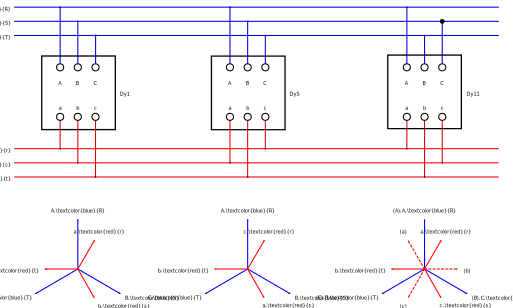
\includegraphics{Imatges/Cap-TrafosPot-Exemple-TR-parallel.pdf}

   \vspace*{1.5cm}
   \hspace{1cm}
   \resizebox{!}{0.8cm}{{\fontfamily{pzc}\selectfont Josep Mollera Barriga}}

\end{titlepage}

      \tableofcontents
      \listoftables
      \listoffigures
      \chapter*{Prefaci} \addcontentsline{toc}{chapter}{Prefaci}

   Voldria dir en primer lloc que no he intentat escriure un tractat complet
   d'electrot\`{e}cnia, d'electr\`{o}nica o de sistemes el\`{e}ctrics de pot\`{e}ncia, sin\'{o} que m\'{e}s aviat
   he volgut
   fer una recopilaci\'{o} de q\"{u}estions te\`{o}riques i pr\`{a}ctiques relacionades amb els camps mencionats
   anteriorment.

   Les fonts d'informaci\'{o} utilitzades en la realitzaci\'{o} d'aquest llibre s\'{o}n molt diverses,
   i inclouen llibres sobre les diferents mat\`{e}ries, articles de revistes o d'Internet,
   apunts de classe d'assignatures impartides a l'\textsf{ETSEIB},\index{ETSEIB} i d'altres.

   Pel que fa al llibre en si mateix, ha estat escrit utilitzant el sistema de composici\'{o} de
   textos \LaTeX,\index{LaTex@\LaTeX} el qual
   permet integrar molt f\`{a}cilment text, f\'{o}rmules i gr\`{a}fics, obtenint un resultat de
   gran qualitat. S'han utilitzat diversos paquets d'ampliaci\'{o}, com ara
   l'\AmS-\LaTeX,\index{AmSLaTex@\AmS-\LaTeX}
   per tal de millorar la presentaci\'{o} de certes parts del
   llibre, com per exemple les taules, les cap\c{c}aleres i les f\'{o}rmules matem\`{a}tiques. S'ha utilitzat la distribuci\'{o} MiK\TeX, que ofereix una implementaci\'{o} lliure de \LaTeX , accessible a l'adre\c{c}a: \href{http://www.miktex.org/}{www.miktex.org}.

   Aquest llibre, est\`{a} pensat per ser utilitzat tant de forma directa en la pantalla d'un
   ordinador com en paper despr\'{e}s d'haver-lo impr\`{e}s; per tal d'estalviar paper, el text
   t\'{e} un format pensat per ser impr\`{e}s en paper DIN-A4,\index{DIN-A4} a dues cares.

    El contingut del llibre \'{e}s molt divers, i va des de temes for\c{c}a te\`{o}rics fins a
    d'altres bastant m\'{e}s pr\`{a}ctics. He procurat donar exemples de tots els conceptes
    que s'hi expliquen, excepci\'{o} feta dels molt elementals, perqu\`{e} crec que \'{e}s important
     no quedar-se tan sols amb la teoria de  la resoluci\'{o} d'un problema determinat, sin\'{o} que
     \'{e}s molt \'{u}til veure exemples resolts pas a pas.

    Encara que he fet tots els esfor\c{c}os possibles per eliminar qualsevol
    mena  d'error en aquest text, \'{e}s gaireb\'{e} inevitable que n'hagi quedat algun,
    per tant, si alg\'{u} troba algun error far\`{a} b\'{e} d'avisar-me!


   \'{U}nicament em resta dir que espero que els que llegeixin aquest llibre el trobin
   \'{u}til i interessant.

\vspace*{1cm}
\hfill
\begin{minipage}[b]{25mm}
    
\includegraphics{Imatges/Pre-Prefaci-JMB.pdf}
\end{minipage}

{\large

\hfill \textbf{\textsl{Josep Mollera Barriga}}

\hfill \textbf{\textsl{Badalona, 24 de mar\c{c} de 2014}}

\hfill \href{mailto:jmollerab@ya.com}{\Letter\hspace{2mm}josep.mollerab@ovi.com}

}

      \chapter*{Historial}
\addcontentsline{toc}{chapter}{Historial}

Es presenta a continuaci\'{o} l'evoluci\'{o} que ha tingut aquest llibre, en
les successives versions que han aparegut.

\section*{Versi\'{o} 1.0 (8 de gener de 2005)}
\addcontentsline{toc}{section}{Versi\'{o} 1.0}

Despr\'{e}s de molts esfor\c{c}os, surt a la llum la primera versi\'{o} d'aquest
llibre, format pels cap\'{\i}tols 1, 2, 3, 4, 5, 6 i 7, i els ap\`{e}ndixs A,
B, C, D i E.

\section*{Versi\'{o} 1.1 (8 de febrer de 2005)}
\addcontentsline{toc}{section}{Versi\'{o} 1.1}

S'afegeix al llibre aquest apartat {"<}Historial{">}.

En l'apartat {"<}Notaci\'{o}{">}, s'especifica que el m\`{o}dul d'un nombre
complex \'{e}s igual a l'arrel quadrada \emph{positiva} de la suma dels
quadrats de les seves parts real i imagin\`{a}ria.

Es modifiquen les equacions \eqref{eq:p_3f_34} i \eqref{eq:q_3f_34}.

S'amplia la secci\'{o} corresponent a les difer\`{e}ncies entre les
normatives \textsf{CEI} i \textsf{ANSI}, que fan refer\`{e}ncia als
transformadors de mesura i protecci\'{o} (secci\'{o}
\ref{sec:comp_tt_ti_cei_ansi}).

Es revisa tot el text, fent-hi algunes petites modificacions i
correccions.

\section*{Versi\'{o} 1.2 (16 d'abril de 2005)}
\addcontentsline{toc}{section}{Versi\'{o} 1.2}

En l'apartat {"<}Notaci\'{o}{">}, s'afegeix l'explicaci\'{o} de la convenci\'{o}
seguida a l'hora de dibuixar les fletxes que representen les
tensions i els corrents.

S'afegeix l'ap\`{e}ndix F, on s'explica la designaci\'{o} de les classes de
refrigeraci\'{o} en els transformadors de pot\`{e}ncia.

\section*{Versi\'{o} 1.3 (24 d'octubre de 2005)}
\addcontentsline{toc}{section}{Versi\'{o} 1.3}

Els ap\`{e}ndixs A a F de la versi\'{o} 1.2, es desplacen tres lletres cap
avall, passant a ser els ap\`{e}ndixs D a I respectivament.

S'afegeix un nou ap\`{e}ndix A, dedicat a l'alfabet grec.

S'afegeix un nou ap\`{e}ndix B, dedicat al sistema internacional
d'unitats (SI).

S'afegeix un nou ap\`{e}ndix C, dedicat a les constants f\'{\i}siques.

En l'apartat {"<}Notaci\'{o}{">}, s'amplien les definicions corresponents al
conjugat i al m\`{o}dul d'un nombre complex, i s'inclouen les
definicions de $\mcmplx{V}^*$ i $\hermit{V}$.

S'ha ampliat la secci\'{o} \ref{sec:pot_complex}, corresponent a la
pot\`{e}ncia complexa.

 S'ha ampliat l'exemple de la secci\'{o}
\ref{sec:seccio_pu}.

En la secci\'{o} \ref{sec:EZS}, s'ha afegit el c\`{a}lcul de $R\ped{P}$ i
$\cmplx{Z}\ped{S}$.

 A l'hora de referir-se a la
relaci\'{o} de transformaci\'{o} d'un transformador, se substitueix el
s\'{\i}mbol {"<}$\ddot{u}${">} emprat en les versions anteriors, pel s\'{\i}mbol
{"<}$m${">}.

\section*{Versi\'{o} 1.4 (2 de desembre de 2005)}
\addcontentsline{toc}{section}{Versi\'{o} 1.4}

Es representa correctament la Figura \ref{pic:acobl}, ja que estava
tallada per la dreta.

Es corregeix l'equaci\'{o} \eqref{eq:cdt_trif_exact} i l'exemple que hi
ha a continuaci\'{o}, el qual en fa \'{u}s.

Es revisa tot el text, fent-hi algunes correccions.

\section*{Versi\'{o} 2.0 (3 d'agost de 2006)}
\addcontentsline{toc}{section}{Versi\'{o} 2.0}

S'ha modificat el criteri de colors utilitzat, a l'hora de ressaltar
els enlla\c{c}os interns del document (equacions, p\`{a}gines, etc.) i els
enlla\c{c}os externs; ara els enlla\c{c}os interns s\'{o}n de
\textcolor{red}{color vermell}, i els enlla\c{c}os externs s\'{o}n de
\textcolor{magenta}{color magenta}. A m\'{e}s totes els encap\c{c}alaments
de cap\'{\i}tols, seccions,
 subseccions, taules  i figures, s\'{o}n ara de
 \textcolor{NavyBlue}{color blau}.

S'han afegit nous cap\'{\i}tol i s'ha fet una reordenaci\'{o} que afecta a
diversos cap\'{\i}tols i ap\`{e}ndixs, segons es detalla a continuaci\'{o}:
\begin{dinglist}{'167}
   \item Els cap\'{\i}tols 1 i 2  de la versi\'{o} 1.4 mantenen la seva posici\'{o}.
   \item S'afegeix un nou cap\'{\i}tol 3, on es tracten les s\`{e}ries de Fourier.
   \item S'afegeix un nou cap\'{\i}tol 4, on es tracta la transformada de Laplace.
   \item El cap\'{\i}tol 3 de la versi\'{o} 1.4 es despla\c{c}a dos n\'{u}meros cap
    avall, passant a ser el cap\'{\i}tol 5.
   \item L'ap\`{e}ndix E de la versi\'{o} 1.4 es converteix en el cap\'{\i}tol 6.
   \item Els cap\'{\i}tols 4, 5, 6 i 7  de la versi\'{o} 1.4 es desplacen tres n\'{u}meros cap
    avall, passant a ser els cap\'{\i}tols 7, 8, 9 i 10 respectivament.
    \item L'ap\`{e}ndix G de la versi\'{o} 1.4 es converteix en el cap\'{\i}tol 11.
    \item Els ap\`{e}ndixs A, B, C i D de la versi\'{o} 1.4 mantenen la seva posici\'{o}.
    \item S'afegeix un nou ap\`{e}ndix E, on es tracten relacions trigonom\`{e}triques.
    \item L'ap\`{e}ndix F de la versi\'{o} 1.4 mant\'{e} la seva posici\'{o}.
    \item Els ap\`{e}ndixs H i I de la versi\'{o} 1.4 es desplacen una lletra cap
    amunt, passant a ser els ap\`{e}ndixs G i H respectivament.
\end{dinglist}


 A l'hora de referir-se a la font de corrent i a l'admit\`{a}ncia d'un circuit equivalent
 Norton, se substitueix el sub\'{\i}ndex {"<}Th{">} emprat en les versions
anteriors, pel sub\'{\i}ndex {"<}No{">}.

En l'apartat {"<}Notaci\'{o}{">} s'afegeixen els s\'{\i}mbols: $\mathbb{N}$,
$\mathbb{Z}$, $\mathbb{Z}^+$,  $\mathbb{Z}^*$, $\mathbb{Z}^-$,
$\mathbb{Q}$, $\mathbb{R}$, $\mathbb{R}^+$, $\mathbb{R}^-$ i
$\mathbb{C}$.

S'ha afegit el teorema de la superposici\'{o} en la secci\'{o}
\ref{sec:teoremes}.


S'ha afegit la bateria en la secci\'{o} \ref{sec:comp_elem}, com a un
dels components elementals d'un circuit el\`{e}ctric.

S'ha afegit la secci\'{o} \ref{sec:val_mitja_ef}, on es defineixen els
valors mitj\`{a} i efica\c{c}, i els factors d'amplitud, de forma i
d'arrissada.

S'ha afegit la secci\'{o} \ref{sec:div_tens_corr}, on es tracten els
circuits divisors de tensi\'{o} i divisors de corrent.

 S'ha modificat l'equaci\'{o} \eqref{eq:resistivitat}
i les taules \ref{taula:param-elc} i \ref{taula:AWG}.

S'ha afegit la secci\'{o} \ref{sec:conex_ti_tt}, on s'explica com
connectar correctament transformadors de corrent i de tensi\'{o}, a
aparells de mesura o de protecci\'{o}.

S'ha millorat l'explicaci\'{o} de la secci\'{o} \ref{sec:control-flux-pot}.

S'ha reestructurat la taula \ref{taula:SI-derivades}.

\section*{Versi\'{o} 2.1 (2 de gener de 2007)}
\addcontentsline{toc}{section}{Versi\'{o} 2.1}

S'adopta la compaginaci\'{o} moderna dels par\`{a}grafs en tot el llibre, consistent en separar-los per una l\'{\i}nia en blanc i en no entrar la primera l\'{\i}nia de text.

S'unifica la representaci\'{o} de les fonts de corrent: un cercle amb una fletxa a dins.

S'afegeix una nota a peu de p\`{a}gina en la secci\'{o} \ref{sec:T_N}, relacionant aquesta secci\'{o} amb la secci\'{o} \ref{sec:xarxes_Zth}.

Es millora l'explicaci\'{o} de la secci\'{o} \ref{sec:seccio_pu}, a l'hora que es trasllada de lloc (en les versions anteriors formava part del cap\'{\i}tol \ref{sec:calc_bas}).

Es millora l'explicaci\'{o} de la secci\'{o} \ref{sec:comp-sim-neutre}.

S'afegeix una nota a peu de p\`{a}gina en la secci\'{o} \ref{sec:EZS}, relacionant aquesta secci\'{o} amb el cap\'{\i}tol \ref{chap:flux_carregues}.

S'amplia la descripci\'{o} de l'equaci\'{o} \eqref{eq:awg_mm2}.

S'afegeix la secci\'{o} \ref{sec:sis_eq_no_lin}, on s'explica com resoldre sistemes d'equacions no lineals amb els programes \textit{Mathematica}${}^\circledR$ i \textit{MATLAB}${}^\circledR$.

Es millora l'explicaci\'{o} de la secci\'{o} \ref{sec:llei-s-c-t}, modificant la figura \ref{pic:llei-s-c-t} i numerant l'equaci\'{o} de la llei dels sinus.

\section*{Versi\'{o} 2.2 (10 de mar\c{c} de 2008)}
\addcontentsline{toc}{section}{Versi\'{o} 2.2}

Es canvia el color dels enlla\c{c}os interns, passant a ser de color negre com el text.

S'afegeixen les unitats que mancaven en alguns exemples.

En la secci\'{o} \ref{sec:MCM} s'introdueixen les unitats cmil i kcmil, equivalents a les unitats CM i MCM respectivament. Avui en dia \'{e}s m\'{e}s freq\"{u}ent veure escrit cmil i kcmil.

Es revisa l'ap\`{e}ndix B utilitzant les publicacions de l'any 2006 del {"<}Bureau
International des Poids et Mesures{">} (\textsf{BIPM}).\index{BIPM}

Es revisa l'ap\`{e}ndix C utilitzant les publicacions de l'any 2006 del {"<}Committee on Data for Science and Technology{">} (\textsf{CODATA}).\index{CODATA}

\section*{Versi\'{o} 3.0 (1 d'octubre de 2008)}
\addcontentsline{toc}{section}{Versi\'{o} 3.0}

Els cap\'{\i}tols 9, 10 i 11 de la versi\'{o} 2.2, es desplacen un n\'{u}mero cap
avall, passant a ser els cap\'{\i}tols 10, 11 i 12 respectivament.

Es crea un nou cap\'{\i}tol 9, dedicat als transformadors de pot\`{e}ncia;
l'ap\`{e}ndix H de la versi\'{o} 2.2 desapareix com a tal, quedant integrat
dins d'aquest nou cap\'{\i}tol.


\section*{Versi\'{o} 3.1 (5 de desembre de 2009)}
\addcontentsline{toc}{section}{Versi\'{o} 3.1}
En l'Ap\`{e}ndix B s'afegeixen els prefixes de pot\`{e}ncies bin\`{a}ries Ki, Mi, Gi, Ti, Pi i Ei.

Es revisa tot el text, fent-hi algunes petites modificacions i
correccions.

\section*{Versi\'{o} 3.2 (5 de gener de 2010)}
\addcontentsline{toc}{section}{Versi\'{o} 3.2}
S'afegeix l'apartat Bibliografia despr\'{e}s del ap\`{e}ndixs. 
      \fancyhf{} \fancyhead[LE,RO]{\sffamily\bfseries\thepage}
      \fancyhead[LO,RE]{\sffamily\bfseries\nouppercase Notaci\'{o}}
      \chapter*{Notació} \addcontentsline{toc}{chapter}{Notació}

\section*{Variables} \addcontentsline{toc}{section}{Variables}


En aquest llibre les variables escalars s'escriuen en lletra  de gruix normal, i  les variables vectorials i matricials s'escriuen
en lletra negreta.

\begin{list}{}
{\setlength{\labelwidth}{15mm} \setlength{\leftmargin}{20mm}
\setlength{\labelsep}{5mm}}
    \item[$j$] La unitat imaginària, definida com:
    $j\equiv\sqrt{-1}$\index{j@$j$}
    \item[$V$] Una variable real.
    \item[$\cmplx{V}$] Una variable complexa.
    \item[$\cmplx{V}^*$] Conjugat d'una variable complexa.
    Es compleixen les relacions:\\[1ex]
     $(\cmplx{V}_1 \pm \cmplx{V}_2 \pm \cdots  \pm \cmplx{V}_n)^* = \cmplx{V}_1^* \pm
    \cmplx{V}_2^*\pm\cdots\pm\cmplx{V}_n^*$\\[1ex]
    $(\cmplx{V}_1 \cmplx{V}_2 \cdots \cmplx{V}_n)^* = \cmplx{V}_1^*  \cmplx{V}_2^*
    \cdots \cmplx{V}_n^*$\\[1ex]
    $(\cmplx{V}_1 / \cmplx{V}_2)^* = \cmplx{V}_1^* / \cmplx{V}_2^*$
    \item[$|\cmplx{V}|$] Mòdul d'una variable complexa.
    Es compleixen les relacions:\\[1ex]
      $\cmplx{V}\,\cmplx{V}^* = |\cmplx{V}|^2$\\[1ex]
      $1/ \cmplx{V} = \cmplx{V}^* / \,|\cmplx{V}|^2$\\[1ex]
      $|\cmplx{V}_1 \cmplx{V}_2 \cdots \cmplx{V}_n| =
       |\cmplx{V}_1| \,|\cmplx{V}_2| \cdots |\cmplx{V}_n|$\\[1ex]
       $|\cmplx{V}_1 / \cmplx{V}_2| = |\cmplx{V}_1| \,/ \,|\cmplx{V}_2|$\\[1ex]
      $|\cmplx{V}_1+\cmplx{V}_2+\cdots+\cmplx{V}_n| \leq
      |\cmplx{V}_1| + |\cmplx{V}_2| + \cdots  +|\cmplx{V}_n|$
    \item[$\arg\cmplx{V}$] Argument (angle) d'una variable complexa.
     Es compleixen les relacions:\\[1ex]
      $\arg\cmplx{V}^* = - \arg\cmplx{V}$\\[1ex]
      $\arg(-\cmplx{V}) =  \arg\cmplx{V} + \piup$\\[1ex]
      $\arg(\cmplx{V}_1 \cmplx{V}_2 \cdots \cmplx{V}_n) = \arg\cmplx{V}_1 + \arg \cmplx{V}_2 + \cdots + \arg\cmplx{V}_n$\\[1ex]
      $\arg(\cmplx{V}_1 / \cmplx{V}_2) = \arg\cmplx{V}_1 - \arg \cmplx{V}_2$
    \item[$\Re\cmplx{V}$] Part real d'una variable complexa. Es compleix: $\Re\cmplx{V} = \dfrac{\cmplx{V} + \cmplx{V}^*}{2}$
    \item[$\Im\cmplx{V}$] Part imaginària d'una variable complexa. Es compleix: $\Im\cmplx{V} = \dfrac{\cmplx{V} - \cmplx{V}^*}{2 j}$
    \item[$A+j B$] Expressió cartesiana (part real i part
    imaginària) d'una variable complexa.
    \item[$Z\angle\theta$] Expressió polar (mòdul i argument) d'una variable
    complexa. Les relacions entre $A, B, Z$ i $\theta$ són:\footnote{Cal tenir en compte que la funció \texttt{arctan} disponible en moltes calculadores i llenguatges de programació, torna de forma  estandarditzada valors compresos entre $-\frac{\piup}{2}$ i $\frac{\piup}{2}$. En aquest cas cal sumar el valor $\piup$, quan $A$ és negatiu, a l'angle obtingut amb la funció \texttt{arctan} per tal d'obtenir l'angle en el quadrant correcte.}\\[1ex]
    $Z=+\sqrt{A^2+B^2}\qquad\quad\theta=\arctan{\dfrac{B}{A}}\qquad\quad
    A=Z\cos\theta\qquad\quad B=Z\sin\theta$
    \item[$Z\,e^{j\theta}$] Expressió d'Euler\index{Euler} d'una variable complexa, definida com:\footnote{El valor de $\theta$ ha d'expressar-se sempre en radian, per tal que el valor de $e^{j\theta}$ sigui correcte.}
     $Z\,e^{j\theta} \equiv Z(\cos\theta+j\sin\theta)$.
     Es compleixen les relacions:\\[1ex]
     $Z_1\,e^{j\theta_1} \, Z_2\,e^{j\theta_2} = Z_1 Z_2\,e^{j(\theta_1+\theta_2)}$\\[1ex]
     %$(Z_1\,e^{j\theta_1}) \,/\, (Z_2\,e^{j\theta_2}) = \dfrac{Z_1}{Z_2}\,e^{j(\theta_1-\theta_2)}$
     $\dfrac{Z_1\,e^{j\theta_1}}{Z_2\,e^{j\theta_2}} = \dfrac{Z_1}{Z_2}\,e^{j(\theta_1-\theta_2)}$
    \item[$\boldsymbol{V}$] Una matriu real o un vector real.
    \item[$\boldsymbol{V}^{-1}$] Matriu inversa d'una matriu real.
    \item[$\transpose{\boldsymbol{V}}$] Matriu transposada d'una matriu real, o vector
    transposat d'un vector real.
    \item[$\boldsymbol{V}(n)$] Element $n$-èsim d'un vector real.
    \item[$\boldsymbol{V}(m,n)$] Element de la fila $m$ i columna $n$ d'una matriu real.
    \item[$\mcmplx{V}$] Una matriu complexa o un vector complex.
    \item[$\mcmplx{V}^{-1}$] Matriu inversa d'una matriu complexa.
    \item[$\transpose{\mcmplx{V}}$] Matriu transposada d'una matriu complexa, o vector
    transposat d'un vector complex.
    \item[$\mcmplx{V}^*$] Matriu conjugada d'una matriu complexa, o vector
    conjugat d'un vector complex.
    \item[$\hermit{V}$] Matriu conjugada transposada d'una matriu complexa, o vector
    conjugat transposat d'un vector complex, definit com: $\hermit{V} \equiv
    \transpose{(\mcmplx{V}^*)}$.
    \item[$\mcmplx{V}(n)$] Element $n$-èsim d'un vector complex.
    \item[$\mcmplx{V}(m,n)$] Element de la fila $m$ i columna $n$ d'una matriu complexa.
\end{list}

Pel que fa als sentits assignats a les fletxes que representen les
tensions i els corrents en els diversos circuits elèctrics que
apareixen en aquest llibre, s'utilitza la convenció següent:

\begin{list}{}
{\setlength{\labelwidth}{15mm} \setlength{\leftmargin}{20mm}
\setlength{\labelsep}{5mm}}
    \item[$\begin{CD} @>U>> \end{CD}$] Tensió contínua: la fletxa indica el sentit
    de la caiguda de tensió, és a dir, va del nus positiu al nus negatiu.
    \item[$\begin{CD} @>I>> \end{CD}$] Corrent
    continu: la fletxa indica el sentit  assignat com a positiu al corrent.
    \item[$\begin{CD} @>\cmplx{U}>> \end{CD}$] Tensió alterna: la fletxa indica el
    sentit assignat com a positiu a la caiguda de tensió, quan el nus d'origen de la fletxa
    té un potencial  més positiu que el nus de destinació.
    \item[$\begin{CD} @>\cmplx{I}>> \end{CD}$] Corrent altern: la fletxa
    indica el sentit  assignat com a positiu al corrent.
\end{list}

\section*{Fasors} \addcontentsline{toc}{section}{Fasors}

En aquest llibre les variables complexes s'utilitzen per representar fasors. Un fasor $Z\angle\theta$ és equivalent a una funció sinusoidal variable en el temps, la qual pot expressar-se utilitzant la funció cosinus:
\[y(t)=\sqrt{2}\, Z \cos(\omega t + \theta)\]

o utilitzant la funció sinus:
\[y(t)=\sqrt{2}\, Z \sin(\omega t + \theta)\]

Quan hi ha diverses funcions sinusoidals relacionades entre si, cal utilitzar de manera uniforme la funció cosinus o la funció sinus per a totes les funcions. Les variables i paràmetres implicats són:
\begin{list}{}
{\setlength{\labelwidth}{15mm} \setlength{\leftmargin}{20mm}
\setlength{\labelsep}{5mm}}
    \item[$y(t)$] Funció sinusoidal; representa normalment una tensió o un corrent.
    \item[$t$] Temps.
    \item[$f$] Freqüència de la funció sinusoidal.
    \item[$T$] Període de la funció sinusoidal.
    \item[$\omega$] Velocitat angular de la funció sinusoidal. Es compleix: $\omega = 2 \piup f = 2 \piup/T$.
    \item[$Z$] Valor eficaç de la funció sinusoidal (vegeu la secció \vref{sec:val_mitja_ef}); els valors de pic de la funció sinusoidal  són:  $\pm\sqrt{2}\, Z$.
    \item[$\theta$] Angle inicial de la funció sinusoidal, on  $\theta=\omega \tau = -\omega (T-\tau)$; el significat del temps $\tau$  es pot veure en el gràfic que hi ha més avall.

    Quan es fa servir la funció cosinus, $\theta$ és positiu quan s'utilitza $\tau$, és a dir, el temps mesurat  des de l'origen ($t=0$) cap a l'esquerra, fins a trobar el primer valor màxim de la funció, i $\theta$ és negatiu quan s'utilitza $T-\tau$, és a dir, el temps mesurat des de l'origen cap a la dreta, fins a trobar també el primer valor màxim de la funció.

    Quan es fa servir la funció sinus, $\theta$ és positiu quan s'utilitza $\tau$, és a dir, el temps mesurat des de l'origen ($t=0$) cap a l'esquerra, fins a trobar el primer punt on la funció es fa zero (passant de valors negatius a positius), i $\theta$ és negatiu quan s'utilitza $T-\tau$, és a dir, el temps mesurat des de l'origen cap a la dreta, fins a trobar també el primer punt on la funció es fa zero (passant de valors negatius a positius).
    \item[] \input{Imatges/Not-Fasor.pdf_tex}
\end{list}
\index{fasor}

\section*{Conjunts de nombres i intervals} \addcontentsline{toc}{section}{Conjunts de nombres i intervals}

Els símbols que representen els diferents conjunts de nombres i intervals, segons la norma internacional ISO 80000-2 
\textit{Quantities and units --- Part 2: Mathematics}, són els següents:

\begin{list}{}
{\setlength{\labelwidth}{15mm} \setlength{\leftmargin}{20mm}
\setlength{\labelsep}{5mm}}
	 \item[$\mathsfb{N}$] Conjunt dels nombres naturals: $\{\,0,1,2,3,4,\ldots\,\}$. 
	 
	 L'exclusió del zero s'indica amb un asterisc: $\mathsfb{N}^* = \{ n \in \mathsfb{N} \mid n \ne 0 \}$. 
	 
	 És possible indicar altres restriccions, com per exemple:  $\mathsfb{N}_{> 5} = \{ n \in \mathsfb{N} \mid n > 5\}$. 
	 
	 També s'utilitzen els símbols $\vmathbb{N}$ i  $\vvmathbb{N}$.
	 
	 \item[$\mathsfb{Z}$] Conjunt dels nombres enters: $\{\,\ldots,-3,-2,-1,0,1,2,3,\ldots\,\}$.  
	 
	 L'exclusió del zero s'indica amb un asterisc: $\mathsfb{Z}^* = \{ n \in \mathsfb{Z} \mid n \ne 0 \}$. 
	 
	 És possible indicar altres restriccions, com per exemple:  $\mathsfb{Z}_{> -3} = \{ n \in \mathsfb{Z} \mid n > -3\}$.     
	 
	 També s'utilitzen els símbols $\vmathbb{Z}$ i $\vvmathbb{Z}$.
    
	 \item[$\mathsfb{Q}$] Conjunt dels nombres racionals. 
	 
	 L'exclusió del zero s'indica amb un asterisc: $\mathsfb{Q}^* = \{ r \in \mathsfb{Q} \mid r \ne 0 \}$. 
	 
	 És possible indicar altres restriccions, com per exemple:  $\mathsfb{Q}_{< 0} = \{ r \in \mathsfb{Q} \mid r < 0 \}$. 
	 
	 També s'utilitzen els símbols $\vmathbb{Q}$ i $\vvmathbb{Q}$.
	 
	 \item[$\mathsfb{R}$] Conjunt dels nombres reals. 
	 
	 L'exclusió del zero s'indica amb un asterisc: $\mathsfb{R}^* = \{ x \in \mathsfb{R} \mid x \ne 0 \}$. 
	 
	 És possible indicar altres restriccions, com per exemple:  $\mathsfb{R}_{> 0} = \{ x \in \mathsfb{R} \mid x > 0 \}$. 
	 
	 També s'utilitzen els símbols $\vmathbb{R}$ i $\vvmathbb{R}$.
	 
	\item[$\mathsfb{C}$] Conjunt dels nombres complexos.  
	
	L'exclusió del zero s'indica amb un asterisc: $\mathsfb{C}^* = \{ z \in \mathsfb{C} \mid z \ne 0 \}$.
	
	 També s'utilitzen els símbols $\vmathbb{C}$ i $\vvmathbb{C}$.
	 
	 \item[$\mathsfb{P}$] Conjunt dels nombres primers: $\{\,2,3,5,7,11,13,17,19,23,29,31,37,41,43,47,53,59,61,\ldots\,\}$. 
	 
	 També s'utilitzen els símbols $\vmathbb{P}$ i $\vvmathbb{P}$.
	 
	 \item[{$[a,b]$}] Interval tancat des de $a$ inclòs fins a $b$ inclòs: $[a,b] = \{x \in \mathsfb{R} \mid a \leq x \leq b\}$.
	 
	 \item[{$(a,b]$}] Interval semiobert esquerre des de $a$ exclòs fins a $b$ inclòs: $(a,b] = \{x \in \mathsfb{R} \mid a < x \leq b\}$. 
	 
	 També s'utilitza la notació $]a,b]$.
	 
	 \item[{$[a,b)$}] Interval semiobert dret des de $a$ inclòs fins a $b$ exclòs: $[a,b) = \{x \in \mathsfb{R} \mid a \leq x < b\}$. 
	 
	 També s'utilitza la notació $[a,b[$.
	 
	 \item[{$(a,b)$}] Interval obert des de $a$ exclòs fins a $b$ exclòs: $(a,b) = \{x \in \mathsfb{R} \mid a < x < b\}$. 
	 
	 També s'utilitza la notació $]a,b[$.
	 
	 \item[{$(-\infty,b]$}] Interval iŀlimitat tancat fins a $b$ inclòs: $(-\infty,b] = \{x \in \mathsfb{R} \mid x \leq b\}$.  
	 
	 També s'utilitza la notació $]-\infty,b]$.
	 
	 \item[{$(-\infty,b)$}] Interval iŀlimitat obert fins a $b$ exclòs: $(-\infty,b) = \{x \in \mathsfb{R} \mid x < b\}$. 
	 
	 També s'utilitza la notació $]-\infty,b[$.
	 
	 \item[{$[a,+\infty)$}] Interval iŀlimitat tancat des de $a$ inclòs: $[a, +\infty) = \{x \in \mathsfb{R} \mid  x \geq a\}$. 
	 
	 També s'utilitzen les notacions $[a, \infty)$, $[a, +\infty[$ i $[a, \infty[$.

	\item[{$(a,+\infty)$}] Interval iŀlimitat obert des de $a$ exclòs: $(a, +\infty) = \{x \in \mathsfb{R} \mid  x > a\}$. 
	
	També s'utilitzen les notacions $(a, \infty)$, $]a, +\infty[$ i $]a, \infty[$.
\end{list}
\index{N@$\mathsfb{N}$} \index{N@$\mathsfb{N}^*$}
\index{Z@$\mathsfb{Z}$} \index{Z@$\mathsfb{Z}^*$}
\index{Q@$\mathsfb{Q}$} \index{Q@$\mathsfb{Q}^*$}
\index{R@$\mathsfb{R}$} \index{R@$\mathsfb{R}^*$}
\index{C@$\mathsfb{C}$} \index{C@$\mathsfb{C}^*$}
\index{P@$\mathsfb{P}$}


\section*{Alfabet grec} \addcontentsline{toc}{section}{Alfabet grec}
\index{alfabet grec}

A continuació es pot veure l'alfabet grec
amb els noms de les seves lletres en diversos idiomes. Algunes lletres minúscules tenen dues grafies, totalment equivalents entre sí.

\begin{center}
\begin{threeparttable}
	\begin{tabular}{cccllll}
		\toprule[1pt]
		\renewcommand*{\multirowsetup}{\centering}
		\multirow{2}{15mm}{\rule{0mm}{4.5mm}Número\\d'ordre} & \multicolumn{2}{c}{Lletra} &
		\multicolumn{4}{c}{Nom} \\
		\cmidrule(rl){2-3} \cmidrule(rl){4-7}
		& minúscula & majúscula & català & castellà &  anglès & francès\\
		\midrule
		1  & $\alphaup$ & A & alfa & alfa &  alpha & alpha\\
		2  & $\betaup$ & B & beta & beta &  beta & bêta\\
		3  & $\gammaup$ & $\Gammaup$ & gamma & gamma &  gamma & gamma\\
		4  & $\deltaup$ & $\Deltaup$ & delta & delta &  delta & delta\\
		5  & $\epsilonup$, $\varepsilonup$ & E & èpsilon & épsilon &  epsilon & epsilon\\
		6  & $\zetaup$ & Z & zeta & dseta &  zeta & zêta\\
		7  & $\etaup$ & H & eta & eta &  eta & êta\\
		8  & $\thetaup$, $\varthetaup$ & $\Thetaup$ & theta & zeta &  theta & thêta\\
		9  & $\iotaup$ & I & iota & iota &  iota & iota\\
		10 & $\kappaup$, $\varkappaup$ & K & kappa & kappa &  kappa & kappa\\
		11 & $\lambdaup$ & $\Lambdaup$ & lambda & lambda &  lambda &lambda\\
		12 & $\muup$ & M & mi & mi &  mu & mu\\
		13 & $\nuup$ & N & ni & ni &  nu & nu\\
		14 & $\xiup$ & $\Xiup$ & ksi & xi &  xi & ksi, xi\\
		15 & o & O & òmicron & ómicron &  omicron & omicron\\
		16 & $\piup$, $\varpiup$\tnote{\color{blue}(a)} & $\Piup$ & pi & pi &  pi & pi\\
		17 & $\rhoup$, $\varrhoup$ & P & rho, ro & ro &  rho & rhô\\
		18 & $\sigmaup$, $\varsigmaup$\tnote{\color{blue}(b)} & $\Sigmaup$ & sigma & sigma &  sigma &sigma\\
		19 & $\tauup$ & T & tau & tau & tau &tau\\
		20 & $\upsilonup$ & $\Upsilonup$ & ípsilon & ípsilon &  upsilon &upsilon\\
		21 & $\phiup$, $\varphiup$ & $\Phiup$ & fi & fi &  phi & phi\\
		22 & $\chiup$ & X & khi & ji &  chi & khi\\
		23 & $\psiup$ & $\Psiup$ & psi & psi &  psi & psi\\
		24 & $\omegaup$ & $\Omegaup$ & omega & omega &  omega & oméga\\
		\bottomrule[1pt]
	\end{tabular}
	\begin{tablenotes}
		\item[\color{blue}(a)] {\footnotesize La variant $\varpiup$ de la lletra pi, que no es fa servir en textos tècnics i científics, es denomina «pi dòrica» en  català, «pi dórica» en castellà, «dorian pi» en anglès, i «pi dorien» en francès.}
		\item[\color{blue}(b)] {\footnotesize En grec, la variant $\varsigmaup$ de la lletra sigma s'escriu  al final d'una paraula, i la variant $\sigmaup$  a l'inici o en mig d'una paraula. En els textos tècnics i científics s'utilitza  la variant $\sigmaup$.}
	\end{tablenotes}
\end{threeparttable}
\end{center}



Els noms d'algunes lletres poden sorprendre, ja que n'hi ha que han rebut històricament noms
diversos, i fins i tot contradictoris respecte dels actuals.

Els noms anglesos de les lletres són els més uniformes, ja que no
s'ha observat cap variació en les diverses fonts consultades, essencialment el diccionari nord-americà Merriam-Webster\footnote{Aquest diccionari es pot consultar a l'adreça: \href{https://www.merriam-webster.com/}{https://www.merriam-webster.com}.} i els diccionaris britànics Oxford\footnote{Aquest diccionari es pot consultar a l'adreça: \href{https://www.oed.com/}{https://www.oed.com}.} i Cambridge.\footnote{Aquest diccionari es pot consultar a l'adreça: \href{https://dictionary.cambridge.org/}{https://dictionary.cambridge.org}.}

Els noms catalans de les lletres són els que apareixen en el \textit{Diccionari de la llengua catalana, 2a edició, 2007} (DIEC2).\footnote{Aquest diccionari es pot consultar a l'adreça: \href{http://dlc.iec.cat/}{https://dlc.iec.cat}. La versió en línia s'actualitza periòdicament.} Altres noms utilitzats en
les diverses fonts consultades, que actualment estan fora de la norma ortogràfica, són:
\begin{multicols}{3}
	\begin{list}{}
		{\setlength{\labelwidth}{16mm} \setlength{\leftmargin}{16mm} \setlength{\labelsep}{2mm}}
		\item[B, $\betaup :$] vita.
		\item[Z, $\zetaup :$] zita.
		\item[H, $\etaup :$] ita.
		\item[$\Thetaup$, $\thetaup :$] thita.
		\item[T, $\tauup :$] taf.
		\item[$\xiup$, $\Xiup$:] csi.\footnote{El nom «csi» apareix juntament amb «ksi» en el \textit{Gran Diccionari de la Llengua Catalana (1999)}. Aquest diccionari es pot consultar a l'adreça:  \href{https://www.diccionari.cat/}{https://www.diccionari.cat}.}
	\end{list}
\end{multicols}

Els noms castellans de les lletres són els que apareixen en el \textit{Diccionario de la Lengua Española, 23ª
	edición, 2014} (D.R.A.E.).\footnote{Aquest diccionari es pot consultar a l'adreça:  \href{https://www.rae.es/}{https://www.rae.es}. La versió en línia s'actualitza periòdicament.} Altres noms utilitzats en les diverses fonts
consultades, que actualment estan fora de la norma ortogràfica, són:
\begin{multicols}{3}
	\begin{list}{}
		{\setlength{\labelwidth}{16mm} \setlength{\leftmargin}{16mm} \setlength{\labelsep}{2mm}}
		\item[Z, $\zetaup :$] zeta,\footnote{\label{fn:zeta}Els noms «zeta», «theta», «my» i «ny» eren els que apareixien en les edicions
			del D.R.A.E anteriors a la 21a (1992).} dseda,\footnote{El nom «dseda» era el que apareixia en l'edició 22a (2001) del D.R.A.E.} dzeta.
		\item[$\Thetaup$, $\thetaup :$] theta,\footnoteref{fn:zeta} thita.
		\item[K, $\kappaup :$] cappa.
		\item[M, $\muup :$] my,\footnoteref{fn:zeta} mu.
		\item[N, $\nuup :$] ny,\footnoteref{fn:zeta} nu.
		\item[O, o :] omicrón.
		\item[P, $\rhoup :$] rho.
		\item[$\Upsilonup$, $\upsilonup :$] úpsilon.
		\item[$\Phiup$, $\phiup :$] phi.
	\end{list}
\end{multicols}

Els noms francesos de les lletres són els que apareixen en el \textit{Dictionnaire de l'Académie française, neuvième édition}.\footnote{Aquest diccionari es pot consultar a l'adreça: \href{https://www.academie-francaise.fr/le-dictionnaire/la-9e-edition}{https://www.academie-francaise.fr/le-dictionnaire/la-9e-edition}.} 
   \mainmatter
      % estil de les p\`{a}gines normals parells i senars
      \renewcommand{\chaptermark}[1]{\markboth{\chaptername\ \thechapter.\ #1}{}}
      \renewcommand{\sectionmark}[1]{\markright{\thesection\ #1}}
      \fancyhf{} \fancyhead[LE,RO]{\sffamily\bfseries\thepage}
      \fancyhead[LO]{\sffamily\bfseries\nouppercase\rightmark}
      \fancyhead[RE]{\sffamily\bfseries\nouppercase\leftmark}
   \part{Electrot\`{e}cnia}
      \chapter{Fonaments}

\section{Introducció}
Es tracten en aquest capítol qüestions bàsiques
d'electrotècnia, com ara teoremes, definicions i relacions, components elementals, i circuits bàsics.


\section{Teoremes d'electrotècnia}\label{sec:teoremes}

\subsection{\texorpdfstring{Teorema de Thévenin--Norton}{Teorema de
            Thévenin-Norton}}\label{sec:T_N}

\index{teorema!de Thévenin}El teorema de Thévenin ens permet
substituir una xarxa complexa formada per elements lineals, per un
circuit equivalent format per una font de tensió $\cmplx{E}\ped{Th}$
en sèrie amb una impedància $\cmplx{Z}\ped{Th}$.


Atenent a la Figura \vref{pic:Thevenin}, si coneixem la tensió en
buit $\cmplx{U}\ped{o}$ entre dos nusos $\alphaup$ i $\betaup$ d'una
xarxa, i la impedància $\cmplx{Z}_{\alphaup\betaup}$ d'aquesta xarxa
vista des d'aquests dos nusos, podem obtenir els valors del circuit
Thévenin equivalent entre aquests dos nusos a partir de les
relacions següents:\index{ETh@$E\ped{Th}$}\index{ZTh@$Z\ped{Th}$}
\begin{equation}
   \cmplx{E}\ped{Th} = \cmplx{U}\ped{o} \qquad\qquad  \cmplx{Z}\ped{Th} = \cmplx{Z}_{\alphaup\betaup}
\end{equation}

D'aquesta manera, la connexió d'aquesta xarxa a través dels nusos
$\alphaup$ i $\betaup$ a una càrrega qualsevol $\cmplx{Z}\ped{Q}$, és
equivalent pel que fa a aquesta càrrega, a connectar-la al circuit
equivalent Thévenin.
\begin{center}
    \input{Imatges/Cap-Fonaments-Thevenin.pdf_tex}
    \captionof{figure}{Teorema de Thévenin}
    \label{pic:Thevenin}
\end{center}

\index{teorema!de Norton}El teorema de Norton ens permet substituir
una xarxa complexa formada per elements lineals, per un circuit
equivalent format per una font de corrent $\cmplx{J}\ped{No}$ en
paraŀlel amb una admitància $\cmplx{Y}\ped{No}$.

Atenent a la Figura \vref{pic:Norton}, si coneixem el corrent de
curtcircuit $\cmplx{I}\ped{cc}$ entre dos nusos $\alphaup$ i $\betaup$
d'una xarxa, i l'admitància $\cmplx{Y}_{\alphaup\betaup}$ d'aquesta
xarxa vista des d'aquests dos nusos, podem obtenir els valors del
circuit Norton equivalent entre aquests dos nusos a partir de les
relacions següents:\index{JNo@$J\ped{No}$}\index{YNo@$Y\ped{No}$}
\begin{equation}
   \cmplx{J}\ped{No} = \cmplx{I}\ped{cc} \qquad\qquad \cmplx{Y}\ped{No} = \cmplx{Y}_{\alphaup\betaup}
\end{equation}

D'aquesta manera, la connexió d'aquesta xarxa a través dels nusos
$\alphaup$ i $\betaup$ a una càrrega qualsevol $\cmplx{Z}\ped{Q}$, és
equivalent pel que fa a aquesta càrrega, a connectar-la al circuit
equivalent Norton.
\begin{center}
    \input{Imatges/Cap-Fonaments-Norton.pdf_tex}
    \captionof{figure}{Teorema de Norton}
    \label{pic:Norton}
\end{center}

Els circuits Thévenin i Norton d'una xarxa són equivalents entre si.
Els paràmetres que defineixen aquests dos circuits compleixen les relacions
següents:
\begin{equation}\label{eq:Thevenin-Norton}
   \cmplx{E}\ped{Th} = \frac{\cmplx{J}\ped{No}}{\cmplx{Y}\ped{No}} \qquad\qquad
   \cmplx{J}\ped{No} = \frac{\cmplx{E}\ped{Th}}{\cmplx{Z}\ped{Th}} \qquad\qquad
    \cmplx{Z}\ped{Th} = \frac{1}{\cmplx{Y}\ped{No}}
\end{equation}

Els valors $\cmplx{Z}\ped{Th}$ i  $\cmplx{Y}\ped{No}$ es poden
obtenir substituint en la xarxa  les fonts de tensió  per curtcircuits, i les fonts de corrent per circuits oberts, i calculant
aleshores la impedància o admitància equivalent\footnote{El càlcul sistemàtic de $\cmplx{Z}\ped{Th}$ i  $\cmplx{Y}\ped{No}$ en una xarxa qualsevol, s'exposa en la secció \ref{sec:xarxes_Zth}}.

\subsection{Teorema de Millman}\label{sec:millman}

\index{teorema!de Millman}Atenent a la Figura \vref{pic:Millman}, el teorema
de Millman ens permet
obtenir la tensió de l'extrem comú $\nuup$ de diverses impedàncies respecte d'un punt
qualsevol $\alphaup$, a partir de les tensions dels altres extrems de les impedàncies respecte
 del mateix punt $\alphaup$.

\hfill
\begin{minipage}[b]{7cm}
    \input{Imatges/Cap-Fonaments-Millman.pdf_tex}
    \captionof{figure}{Teorema de Millman}
    \label{pic:Millman}
\end{minipage}
\hfill
\begin{minipage}[b][4.5cm][t]{6cm}
    \begin{equation}
        \cmplx{U}_{\nuup\alphaup} = \frac{\displaystyle\sum_{k=1}^n \dfrac{\cmplx{U}_{k\alphaup}}{\cmplx{Z}_k}} {\displaystyle\sum_{k=1}^n \dfrac{1}{\cmplx{Z}_k}}
    \end{equation}
\end{minipage}


\pagebreak

\begin{exemple}[Teorema de Millman -- Bateries en paraŀlel]
    A partir de la figura següent, es tracta de determinar els circuits
    Thévenin i Norton equivalents del circuit format per les tres
    bateries i les seves resistències, i calcular la tensió i el
    corrent que existirien en una resistència de càrrega
    $R\ped{Q}=\SI{50}{\ohm}$, que es connectés entre els punts $\alphaup$
    i $\nuup$.

    \begin{center}
        \input{Imatges/Cap-Fonaments-Millman-Exemple1.pdf_tex}
    \end{center}

    La impedància Thévenin equivalent es calcula, tal com s'ha dit en la Secció \ref{sec:T_N},
    substituint en el circuit totes les fonts de tensió per curtcircuits; així doncs, ens
    queden tres resistències en paraŀlel entre $\alphaup$ i $\nuup$:
    \[
    Z\ped{Th} = \frac{1}{\dfrac{1}{\SI{0,034}{\ohm}} +
    \dfrac{1}{\SI{0,041}{\ohm}} + \dfrac{1}{\SI{0,029}{\ohm}}} =
    \SI{0,01133}{\ohm}
    \]

    Per calcular la font de tensió Thévenin equivalent, utilitzarem el
    teorema de Millman. Si es compara aquest circuit amb el de la Figura
    \vref{pic:Millman}, veiem que els punts $\alphaup$ i $\nuup$ dels dos
    circuits són equivalents, és a dir, $\nuup$ és el punt comú de les
    impedàncies, i $\alphaup$ és el punt de referència dels altres extrems
    de les impedàncies, respecte del qual les tensions són conegudes
    (tensions de les bateries). Així doncs tenim:
    \[
    U_{\nuup\alphaup} = \frac{\dfrac{\SI{-125,1}{V}}{\SI{0,034}{\ohm}} +
    \dfrac{\SI{-124,8}{V}}{\SI{0,041}{\ohm}} +
    \dfrac{\SI{-125,2}{V}}{\SI{0,029}{\ohm}}}{\dfrac{1}{\SI{0,034}{\ohm}}
    + \dfrac{1}{\SI{0,041}{\ohm}} + \dfrac{1}{\SI{0,029}{\ohm}}} =
    \SI{-125,0562}{V}
    \]

    La font de tensió  Thévenin equivalent entre $\alphaup$ i $\nuup$ és per
    tant:
    \[
    E\ped{Th} = U_{\alphaup\nuup} = \SI{125,0562}{V}
    \]

    Calculem a continuació l'admitància i la font de corrent  Norton equivalents, utilitzant
    l'equació \eqref{eq:Thevenin-Norton}:
    \begin{align*}
        Y\ped{No} &= \frac{1}{Z\ped{Th}} = \frac{1}{\SI{0,01133}{\ohm}} = \SI{82,2613}{S}
        \\[2ex]
        J\ped{No} &= \frac{E\ped{Th}}{Z\ped{Th}} =
        \frac{\SI{125,0562}{V}}{\SI{0,01133}{\ohm}}= \SI{11037,6150}{A}
    \end{align*}

    Tal com s'ha dit en la Secció \ref{sec:T_N}, J\ped{No} és igual al
    corrent de curtcircuit entre els punts $\alphaup$ i $\nuup$.

    Finalment, ja podem calcular el corrent $I\ped{Q}$ i la tensió $U\ped{Q}$ en la
    resistència de càrrega, utilitzant el circuit Thévenin equivalent calculat anteriorment:
    \begin{align*}
        I\ped{Q} &= \frac{E\ped{Th}}{Z\ped{Th} + R\ped{Q}} = \frac{\SI{125,0562}{V}}
        {\SI{0,01133}{\ohm} + \SI{50}{\ohm}} = \SI{2,5001}{A} \\[2ex]
        U\ped{Q} &=  R\ped{Q} \,I\ped{Q} = \SI{50}{\ohm} \times \SI{2,5001}{A} =
        \SI{125,0050}{V}
    \end{align*}
\end{exemple}


\begin{exemple}[Teorema de Millman -- Càrregues trifàsiques amb corrent de neutre]
    Tenim un generador trifàsic connectat en estrella, amb una tensió fase--neutre de \SI{230}{V}; el punt neutre de l'estrella està connectat a terra a traves d'una resistència de \SI{46}{\ohm}. El generador alimenta tres càrregues resistives connectades entre cadascuna de les fases i terra, de valors \SI{50}{m\ohm}, \SI{80}{m\ohm} i \SI{70}{m\ohm} respectivament. Es tracta de trobar el corrent que circula per la resistència de connexió a terra del generador, i els corrents que circulen per cadascuna de les tres càrregues; és clar que ha de complir-se: $\cmplx{I}\ped{A} + \cmplx{I}\ped{B} + \cmplx{I}\ped{C} = \cmplx{I}\ped{N}$.

    En el dibuix següent es pot veure el circuit elèctric que es vol resoldre.

    \begin{center}
        \input{Imatges/Cap-Fonaments-Millman-Exemple2.pdf_tex}
    \end{center}

    La tensió $\cmplx{U}\ped{GN}$ es pot calcular directament aplicant el teorema de Millman. Per fer-ho, només cal tenir en compte que les quatre resistències del circuit tenen un punt comú que és «G», i que les tensions dels altres extrems de les resistències respecte del punt «N» són conegudes: $\cmplx{U}\ped{AN}=\SIpd{230}{0}{V}$, $\cmplx{U}\ped{BN}=\SIpd{230}{240}{V}$, $\cmplx{U}\ped{CN}=\SIpd{230}{120}{V}$ i  $\cmplx{U}\ped{NN}=\SI{0}{V}$.

    Així doncs tenim:
    \[
    \cmplx{U}\ped{GN} = \frac{ \dfrac{\cmplx{U}\ped{AN}}{R\ped{A}} + \dfrac{\cmplx{U}\ped{BN}}{R\ped{B}} + \dfrac{\cmplx{U}\ped{CN}}{R\ped{C}} + \dfrac{\cmplx{U}\ped{NN}}{R\ped{N}}} { \dfrac{1}{R\ped{A}} + \dfrac{1}{R\ped{B}} + \dfrac{1}{R\ped{C}} + \dfrac{1}{R\ped{N}} } =
    \frac{\dfrac{\SIpd{230}{0}{V}}{\SI{50}{m\ohm}}+\dfrac{\SIpd{230}{240}{V}}{\SI{80}{m\ohm}}+
    \dfrac{\SIpd{230}{120}{V}}{\SI{70}{m\ohm}}}{\dfrac{1}{\SI{50}{m\ohm}}+\dfrac{1}{\SI{80}{m\ohm}}+
    \dfrac{1}{\SI{70}{m\ohm}}+\dfrac{1}{\SI{46}{\ohm}}} =
    \SIpd{33,3433}{13,1736}{V}
    \]

    El corrent  que circula per la resistència de connexió a terra del generador val:
    \[
    \cmplx{I}\ped{N} = \frac{\cmplx{U}\ped{GN}}{R\ped{N}} = \frac{\SIpd{33,3433}{13,1736}{V}}{\SI{46}{\ohm}}
    = \SIpd{0,7249}{13,1736}{A}
    \]

    Finalment, els corrents que circulen per cadascuna de les tres càrregues val:
    \begin{align*}
    \cmplx{I}\ped{A} &= \frac{\cmplx{U}\ped{AG}}{R\ped{A}} = \frac{\cmplx{U}\ped{AN} - \cmplx{U}\ped{GN}}{R\ped{A}} = \frac{\SIpd{230}{0}{V}-\SIpd{33,3433}{13,1736}{V}}{\SI{50}{m\ohm}}
    = \SIpd{3953,6056}{-2,2030}{A}\\[2ex]
    \cmplx{I}\ped{B} &= \frac{\cmplx{U}\ped{BG}}{R\ped{B}} = \frac{\cmplx{U}\ped{BN} - \cmplx{U}\ped{GN}}{R\ped{B}} = \frac{\SIpd{230}{240}{V}-\SIpd{33,3433}{13,1736}{V}}{\SI{80}{m\ohm}}
    = \SIpd{3174,7573}{-125,4941}{A}\\[2ex]
    \cmplx{I}\ped{C} &= \frac{\cmplx{U}\ped{CG}}{R\ped{C}} = \frac{\cmplx{U}\ped{CN} - \cmplx{U}\ped{GN}}{R\ped{C}} = \frac{\SIpd{230}{120}{V}-\SIpd{33,3433}{13,1736}{V}}{\SI{70}{m\ohm}}
    = \SIpd{3453,8265}{127,5857}{A}
    \end{align*}
\end{exemple}

\begin{exemple}[Teorema de Millman -- Càrregues trifàsiques sense corrent de neutre]
    Tenim en aquest cas un circuit com el de l'exemple anterior, però aquí les càrregues no estan connectades a terra (punt G). En aquest cas no hi pot haver circulació de corrent per la resistència de connexió a terra del generador, ja que aquest corrent no tindria cap camí per tancar-se; ha de complir-se doncs: $\cmplx{I}\ped{A} + \cmplx{I}\ped{B} + \cmplx{I}\ped{C} = 0$. Es tracta de trobar en aquest cas els corrents que circulen per cadascuna de les tres càrregues.

    En el dibuix següent es pot veure el circuit elèctric que es vol resoldre.

    \begin{center}
        \input{Imatges/Cap-Fonaments-Millman-Exemple3.pdf_tex}
    \end{center}

    La tensió $\cmplx{U}\ped{KN}$ es pot calcular directament aplicant el teorema de Millman. Per fer-ho, només cal tenir en compte que les tres resistències del circuit tenen un punt comú que és «K», i que les tensions dels altres extrems de les resistències respecte del punt «N» són conegudes: $\cmplx{U}\ped{AN}=\SIpd{230}{0}{V}$, $\cmplx{U}\ped{BN}=\SIpd{230}{240}{V}$ i $\cmplx{U}\ped{CN}=\SIpd{230}{120}{V}$.

    Així doncs tenim:
    \[
    \cmplx{U}\ped{KN} = \frac{ \dfrac{\cmplx{U}\ped{AN}}{R\ped{A}} + \dfrac{\cmplx{U}\ped{BN}}{R\ped{B}} + \dfrac{\cmplx{U}\ped{CN}}{R\ped{C}}} { \dfrac{1}{R\ped{A}} + \dfrac{1}{R\ped{B}} + \dfrac{1}{R\ped{C}}} =
    \frac{\dfrac{\SIpd{230}{0}{V}}{\SI{50}{m\ohm}}+\dfrac{\SIpd{230}{240}{V}}{\SI{80}{m\ohm}}+
    \dfrac{\SIpd{230}{120}{V}}{\SI{70}{m\ohm}}}{\dfrac{1}{\SI{50}{m\ohm}}+\dfrac{1}{\SI{80}{m\ohm}}+
    \dfrac{1}{\SI{70}{m\ohm}}} =
    \SIpd{33,3588}{13,1736}{V}
    \]


    Els corrents que circulen per cadascuna de les tres càrregues val:
    \begin{align*}
    \cmplx{I}\ped{A} &= \frac{\cmplx{U}\ped{AK}}{R\ped{A}} = \frac{\cmplx{U}\ped{AN} - \cmplx{U}\ped{KN}}{R\ped{A}} = \frac{\SIpd{230}{0}{V}-\SIpd{33,3588}{13,1736}{V}}{\SI{50}{m\ohm}}
    = \SIpd{3953,3068}{-2,2042}{A}\\[2ex]
    \cmplx{I}\ped{B} &= \frac{\cmplx{U}\ped{BK}}{R\ped{B}} = \frac{\cmplx{U}\ped{BN} - \cmplx{U}\ped{KN}}{R\ped{B}} = \frac{\SIpd{230}{240}{V}-\SIpd{33,3588}{13,1736}{V}}{\SI{80}{m\ohm}}
    = \SIpd{3174,9027}{-125,4964}{A}\\[2ex]
    \cmplx{I}\ped{C} &= \frac{\cmplx{U}\ped{CK}}{R\ped{C}} = \frac{\cmplx{U}\ped{CN} - \cmplx{U}\ped{KN}}{R\ped{C}} = \frac{\SIpd{230}{120}{V}-\SIpd{33,3588}{13,1736}{V}}{\SI{70}{m\ohm}}
    = \SIpd{3453,9180}{127,5891}{A}
    \end{align*}
\end{exemple}


\subsection{Teorema de la superposició}\index{teorema!de la
superposició}

Si tenim un circuit lineal on hi ha diverses fonts de tensió i  de
corrent, les quals originen corrents i caigudes de tensió en els
components del circuit, el teorema de la superposició ens diu que
podem calcular aquests corrents i caigudes de tensió, resolent els
circuits que resulten de tenir en compte  només una font de tensió o
de corrent a l'hora, i sumant al final els valors parcials
obtinguts.

En cada pas on considerem només una font de tensió o de corrent, hem
d'eliminar la resta de fonts del circuit; per tal de fer-ho hem de
substituir la resta de fonts de tensió per un curtcircuit, i la
resta de fonts de corrent per un circuit obert.

Aquest teorema també és aplicable en el cas que tinguem només una
font de tensió o de corrent, que operi a més d'una freqüència a
l'hora. En aquest cas es pot estudiar el circuit de forma
independent per a cadascuna de les freqüències presents, i sumar al
final els valors parcials obtinguts.

\begin{exemple}[Aplicació del teorema de la superposició]
    Es tracta de trobar en el circuit següent el corrent $\cmplx{I}$ que circula
    pel condensador, utilitzant el teorema de la superposició.
    \begin{center}
        \input{Imatges/Cap-Fonaments-Exemple-Superposicio-1.pdf_tex}
    \end{center}

    Utilitzant el teorema de la superposició, representem els dos
    circuits següents a partir del circuit original. El circuit de
    l'esquerra només té la font de tensió, amb la font de corrent
    substituïda per un circuit obert, i el circuit de
    la dreta només té la font de corrent, amb la font de tensió
    substituïda per un curtcircuit.
    \begin{center}
        \input{Imatges/Cap-Fonaments-Exemple-Superposicio-2.pdf_tex}
    \end{center}

    Els corrents $\cmplx{I}_1$ i $\cmplx{I}_2$ que circulen pel condensador valen:
    \[
        \cmplx{I}_1 = \frac{\SIpd{5}{0}{V}}{\SI{4-2j}{\ohm}} =
        \SIpd{1,118}{26,57}{A} \qquad\qquad
        \cmplx{I}_2 = \frac{\SI{4}{\ohm}}{\SI{4-2j}{ \ohm}} \, \SIpd{2}{0}{A} = \SIpd{1,789}{26,57}{A}
    \]

    El corrent total $\cmplx{I}$ que circula pel condensador val:
    \[
        \cmplx{I}  = \cmplx{I}_1 + \cmplx{I}_2 = \SIpd{1,118}{26,57}{A} +  \SIpd{1,789}{26,57}{A} =
        \SIpd{2,907}{26,57}{A}
    \]
\end{exemple}



\section{Valors mitjà i eficaç, i factors de cresta, de forma i
d'arrissada}\label{sec:val_mitja_ef}

S'explica a continuació com obtenir diversos paràmetres característics de funcions periòdiques  en el temps $v(t)$, de freqüència $f$, període $T$ i velocitat angular $\omega$; les relacions que compleixen aquests tres paràmetres són: $f = 1/T$, $\omega=2\piup f = 2\piup\,/T$.

En la Figura \vref{pic:val-mitja} es representa una funció periòdica qualsevol $v(t)$, indicant-hi el període $T$, els valors mitjà $\bar{V}$, de cresta $\hat{V}$ i de vall $\check{V}$, i la màxima amplitud  $\hat{V}-\check{V}$.
\begin{center}
    \input{Imatges/Cap-Fonaments-Valor-Mitja.pdf_tex}
    \captionof{figure}{Paràmetres d'una funció periòdica}
    \label{pic:val-mitja}
\end{center}

Les funcions periòdiques poden  definir-se en funció de l'angle $\alpha$, enlloc del temps $t$; es compleixen les relacions:
$\alpha=\omega t$, $\diff\alpha=\omega\diff t$.

\subsection{Valor mitjà}

El valor mitjà $\bar{V}$ d'una funció
periòdica en el temps $v(t)$ es
defineix com\footnote{En la Secció \ref{sec:four_val_av} es defineix el valor mitjà d'una funció periòdica expressada en sèries de Fourier.}:
\begin{equation}
    \bar{V} = \frac{1}{T} \int_{t_0}^{t_0+T} v(t) \diff t =
    \frac{\omega}{2\piup} \int_{t_0}^{t_0+\frac{2\piup}{\omega}} v(t) \diff t\label{eq:vm_t}
\end{equation}

Si la funció periòdica $v(\alpha)$ està definida en funció de
l'angle $\alpha$, enlloc del temps $t$, tenim:
\begin{equation}
    \bar{V} = \frac{1}{2\piup} \int_{\alpha_0}^{\alpha_0+2\piup} v(\alpha) \diff \alpha
    \label{eq:vm_alfa}
\end{equation}

\subsection{Valor eficaç}\index{valor!eficaç}
\index{root mean square@\guillemotleft root mean
square\guillemotright}\index{rms}

El valor eficaç  $V$ (també anomenat valor rms, de l'anglès «root
mean square») d'una funció periòdica en el temps $v(t)$ es defineix com\footnote{En la Secció \ref{sec:four_val_ef} es defineix el valor eficaç d'una funció periòdica expressada en sèries de Fourier.}:
\begin{equation}
    V = \sqrt{\frac{1}{T} \int_{t_0}^{t_0+T} [v(t)]^2 \diff
    t} = \sqrt{\frac{\omega}{2\piup} \int_{t_0}^{t_0+\frac{2\piup}{\omega}}
     [v(t)]^2 \diff t}
\end{equation}

Si la funció periòdica $v(\alpha)$ està definida en funció de
l'angle $\alpha$, enlloc del temps $t$, tenim:
\begin{equation}
    V = \sqrt{\frac{1}{2\piup} \int_{\alpha_0}^{\alpha_0+2\piup}
     [v(\alpha)]^2 \diff \alpha}
\end{equation}

\subsection{Factor de cresta}
\index{factor!de cresta}

El factor de cresta relaciona els valors de cresta $\hat{V}$
  i eficaç $V$ d'una funció periòdica. La norma CEI 60050 l'anomena «peak factor» i el defineix com:\index{CEI!60050-00@60050}
\begin{equation}
     \frac{\hat{V}}{V}
\end{equation}

\subsection{Factor de forma}\index{factor!de forma}\index{F@$F$}

El factor de forma relaciona els valors eficaç $V$
i mitjà $\bar{V}$ d'una funció periòdica. La norma CEI 60050 l'anomena «form factor», li assigna el símbol $F$ i el defineix com:\index{CEI!60050-00@60050}
\begin{equation}
    F = \frac{V}{|\bar{V}|}
\end{equation}

\subsection{Factor d'arrissada eficaç}\index{factor!d'arrissada eficaç}\index{r@$r$}

El factor d'arrissada eficaç relaciona els
valors mitjà $\bar{V}$ i eficaç $V$ d'una funció periòdica.
La norma CEI 60050 l'anomena «rms-ripple factor» o «relative ripple content», li assigna el símbol $r$ i el defineix com\footnote{En la Secció \ref{sec:four_fac_arr_ef} es defineix el factor d'arrissada eficaç d'una funció periòdica expressada en sèries de Fourier.}:\index{CEI!60050-00@60050}
\begin{equation}
    r = \sqrt{\frac{V^2}{\bar{V}^2}-1} = \sqrt{F^2-1}\label{eq:rms_rip}
\end{equation}

Aquest factor s'utilitza usualment per definir la qualitat d'una
tensió continua, rectificada a partir d'una tensió alterna; com més
plana sigui aquesta tensió contínua més baix serà el seu factor
d'arrissada.

\subsection{Factor d'arrissada de cresta}\index{factor!d'arrissada de cresta}\index{q@$q$}

El factor d'arrissada de cresta relaciona els valors de cresta $\hat{V}$, de vall $\check{V}$  i mitjà $\bar{V}$
 d'una funció periòdica. La norma CEI 60050 l'anomena «peak-ripple factor» o «peak distortion», li assigna el símbol $q$ i el defineix com:\index{CEI!60050-00@60050}
\begin{equation}
    q = \frac{\hat{V} - \check{V}}{|\bar{V}|}
\end{equation}

\begin{exemple}[Càlcul de factors de cresta, de forma i d'arrissada]
    Es tracta de calcular els factors de cresta, de forma, i d'arrissada eficaç i de cresta,
    de la tensió  que s'obté a partir d'una tensió sinusoïdal
    $u(t) = \hat{U} \sin\omega t$, amb un rectificador de mitja ona i
    amb un rectificador d'ona completa.

    En el cas del rectificador de mitja ona, la tensió que s'obté ve
    definida per:
    \[
    u(t) = \begin{cases} \hat{U} \sin\omega t, & 0 < \omega t < \piup\\
           0, & \piup \leq \omega t \leq 2\piup \end{cases}
    \]

    Calculem en primer lloc el valor mitjà:
    \[
    \bar{U} = \frac{\omega}{2\piup} \left( \int_0^\frac{\piup}{\omega}
    \hat{U} \sin\omega t \diff t +
    \int_\frac{\piup}{\omega}^\frac{2\piup}{\omega} 0 \diff t \right) = -
    \left. \frac{\hat{U} \cos\omega t}{2\piup}
    \right|_0^\frac{\piup}{\omega} = \frac{\hat{U}}{\piup}
    \]

    Calculem a continuació el valor eficaç:
    \[
    U = \sqrt{\frac{\omega}{2\piup} \left( \int_0^\frac{\piup}{\omega}
    \hat{U}^2 \sin^2\omega t \diff t +
    \int_\frac{\piup}{\omega}^\frac{2\piup}{\omega} 0 \diff t \right)} =
      \sqrt{\left.\frac{\omega \hat{U}^2}{2\piup}\left( \frac{t}{2} -
    \frac{\sin (2\omega t)}{4\omega}
    \right)\right|_0^\frac{\piup}{\omega}} = \frac{\hat{U}}{2}
    \]

    Els factors de cresta, de forma, i d'arrissada eficaç i de cresta, són:
    \begin{align*}
        \text{factor de cresta} &= \frac{\hat{U}}{\hat{U}/2} = 2 \\[0.5ex]
        F &= \frac{\hat{U}/2}{\hat{U}/\piup} =\frac{\piup}{2} =
        \num{1,57} \\[0.5ex]
        r &= \sqrt{\left(\frac{\hat{U}/2}{\hat{U}/\piup}\right)^2-1} =
    \sqrt{\frac{\piup^2}{4}-1} = \num{1,21} \\[0.5ex]
        q &= \frac{\hat{U} - 0}{\hat{U}/\piup} = \piup = \num{3,14}
    \end{align*}


    En el cas del rectificador d'ona completa, la tensió que s'obté ve
    definida per:
    \[
    u(t) = \begin{cases} \phantom{-}\hat{U} \sin\omega t, & 0 < \omega t < \piup\\
           -\hat{U} \sin\omega t, & \piup \leq \omega t \leq 2\piup \end{cases}
    \]

    En aquest cas, l'ona de tensió entre $\piup$ i $2\piup$ és una repetició
    exacta de l'ona de tensió entre 0 i $\piup$, per tant, únicament
    caldrà considerar-ne la primera meitat (entre 0 i $\piup$), tenint en
    compte que el període serà $\piup\,/\omega$.

     Calculem en primer lloc el valor mitjà:
    \[
    \bar{U} = \frac{\omega}{\piup} \int_0^\frac{\piup}{\omega} \hat{U}
    \sin\omega t \diff t  = - \left. \frac{\hat{U} \cos\omega t}{\piup}
    \right|_0^\frac{\piup}{\omega} = \frac{2 \hat{U}}{\piup}
    \]

    Calculem a continuació el valor eficaç:
    \[
    U = \sqrt{\frac{\omega}{\piup} \int_0^\frac{\piup}{\omega} \hat{U}^2
    \sin^2\omega t \diff t } =   \sqrt{\left.\frac{\omega
    \hat{U}^2}{\piup}\left( \frac{t}{2} - \frac{\sin (2\omega t)}{4\omega}
    \right)\right|_0^\frac{\piup}{\omega}}  = \frac{\hat{U}}{\sqrt{2}}
    \]

    Els factors de cresta, de forma, i d'arrissada eficaç i de cresta, són:
    \begin{align*}
        \text{factor de cresta} &= \frac{\hat{U}}{\hat{U}/\sqrt{2}} = \sqrt{2} =\num{1,41} \\[0.5ex]
        F &= \frac{\hat{U}/\sqrt{2}}{2 \hat{U}/\piup} =\frac{\piup}{2\sqrt{2}} =
        \num{1,11} \\[0.5ex]
    r &= \sqrt{\left(\frac{\hat{U}/\sqrt{2}}{2 \hat{U}/\piup}\right)^2-1}
    = \sqrt{\frac{\piup^2}{8}-1} = \num{0,48}\\[0.5ex]
    q &=  \frac{\hat{U} - 0}{2 \hat{U}/\piup} = \frac{\piup}{2} = \num{1,57}
    \end{align*}
\end{exemple}

\section{Potència complexa}\label{sec:pot_complex} \index{potència complexa}

\subsection{Potència monofàsica} \index{potència complexa!monofàsica}

En la Figura \vref{pic:pot_comp_mono} es representa una càrrega $\cmplx{Z}=R+\ju X$, la
qual absorbeix una potència complexa $\cmplx{S} = P + \ju Q$.
\begin{center}
    \input{Imatges/Cap-Fonaments-Potencia-Monof.pdf_tex}
    \captionof{figure}{Potència complexa monofàsica}
    \label{pic:pot_comp_mono}
\end{center}

$R$ i $X$ són respectivament la part resistiva i la part reactiva
(inductiva o capacitiva) de la càrrega, i $P$ i $Q$ són
respectivament la potencia activa i la potencia reactiva (inductiva
o capacitiva) absorbida per la càrrega.

La potència activa absorbida per una càrrega sempre és positiva, en
canvi, la potència reactiva absorbida per una càrrega pot ser
positiva o negativa, segons que predomini més la part inductiva o la
part capacitiva de la càrrega respectivament.

L'angle $\varphiup$ entre els fasors $\cmplx{U}$ i $\cmplx{I}$ compleix la següent relació:
\begin{equation}
   \tan\varphiup = \frac{X}{R} = \frac{Q}{P}
\end{equation}

\index{factor!de potència}A partir d'aquest angle $\varphiup$, es
defineix el factor de potència de la càrrega:
\begin{equation}
   \text{Factor de potència} \equiv \cos\varphiup
\end{equation}

Atès que per a un angle qualsevol $\alphaup$ es compleix la igualtat
trigonomètrica: $\cos\alphaup = \cos(-\alphaup)$, quan es dóna el factor
de potència d'una càrrega, cal especificar si és inductiu ($Q>0,
\tan\varphiup>0$) o capacitiu ($Q<0, \tan\varphiup<0$); això es fa
afegint «(i)» o «(c)» respectivament al valor numèric del factor
de potència, com per exemple: $\cos\varphiup=0,8$(i),
$\cos\varphiup=0,9$(c).

Les relacions que lliguen la potència complexa amb la tensió i el corrent són:
\begin{align}
   \cmplx{S} &=  \cmplx{U} \,\cmplx{I}^* =
   |\cmplx{I}|^2 \,\cmplx{Z} = \frac{|\cmplx{U}|^2}{\cmplx{Z}^*} =
   P + \ju Q \label{eq:s_mono1}\\
   |\cmplx{S}| &= |\cmplx{U}| \,|\cmplx{I}| =
   |\cmplx{I}|^2 \,|\cmplx{Z}| = \frac{|\cmplx{U}|^2}{|\cmplx{Z}|} =
   \sqrt{P^2+Q^2} \\
   P &= \Re (\cmplx{U} \, \cmplx{I}^*) = |\cmplx{S}| \cos\varphiup =
   |\cmplx{U}|\, |\cmplx{I}| \cos\varphiup = |\cmplx{I}|^2 R =
   \frac{|\cmplx{U}|^2}{|\cmplx{Z}|^2}R\\
   Q &= \Im (\cmplx{U} \, \cmplx{I}^*) = |\cmplx{S}| \sin\varphiup =
   |\cmplx{U}| \,|\cmplx{I}|\sin\varphiup  = |\cmplx{I}|^2 X =
   \frac{|\cmplx{U}|^2}{|\cmplx{Z}|^2}X
\end{align}

\subsection{Potència trifàsica} \index{potència complexa!trifàsica} \label{sec:pot-trif}

En la Figura \vref{pic:pot_comp_trif} es representen dos sistemes
d'alimentació a càrregues trifàsiques; el de l'esquerra és un
sistema de 4 fils (3 fases + neutre) i el de la dreta és un sistema
de 3 fils (3 fases). En ambdós casos es consideren tres càrregues
$\cmplx{Z}\ped{A} = R\ped{A} + \ju X\ped{A}$, $\cmplx{Z}\ped{B}=
R\ped{B} + \ju X\ped{B}$ i $\cmplx{Z}\ped{C}= R\ped{C} + \ju X\ped{C}$
connectades en estrella, les quals absorbeixen respectivament unes
potències complexes $\cmplx{S}\ped{A} = P\ped{A} + \ju Q\ped{A}$,
$\cmplx{S}\ped{B}= P\ped{B} + \ju Q\ped{B}$ i $\cmplx{S}\ped{C}=
P\ped{C} + \ju Q\ped{C}$.

$R\ped{A}$, $R\ped{B}$ i $R\ped{C}$, i $X\ped{A}$, $X\ped{B}$ i
$X\ped{C}$ són respectivament les parts resistives i les parts
reactives (inductives o capacitives) de les càrregues, i $P\ped{A}$,
$P\ped{B}$ i $P\ped{C}$, i $Q\ped{A}$, $Q\ped{B}$ i $Q\ped{C}$ són
respectivament les potencies actives i les potencies reactives
(inductives o capacitives) absorbides per les càrregues.

El sistema d'alimentació de 3 fils admet també càrregues
trifàsiques connectades en triangle; en aquest cas només cal dur a
terme la transformació a una connexió en estrella (vegeu la Secció
\ref{secc:d_y}), i per tant, la descripció que segueix es pot
considerar del tot general.

\begin{center}
    \input{Imatges/Cap-Fonaments-Potencia-Trif.pdf_tex}
    \captionof{figure}{Potència complexa trifàsica -- Sistemes de 4 fils i 3 fils}
    \label{pic:pot_comp_trif}
\end{center}

En el cas més general, on la càrrega trifàsica és desequilibrada,
cada impedància té el seu propi factor de potència
$\cos\varphiup\ped{A}$, $\cos\varphiup\ped{B}$ i $\cos\varphiup\ped{C}$,
complint-se:
\begin{equation}
    \tan\varphiup\ped{A} = \frac{X\ped{A}}{R\ped{A}} = \frac{Q\ped{A}}{P\ped{A}} \qquad
    \tan\varphiup\ped{B} = \frac{X\ped{B}}{R\ped{B}} = \frac{Q\ped{B}}{P\ped{B}} \qquad
    \tan\varphiup\ped{C} = \frac{X\ped{C}}{R\ped{C}} = \frac{Q\ped{C}}{P\ped{C}}
\end{equation}

\subsubsection{Sistema equilibrat o desequilibrat de 3 fils o de 4 fils}

Aquest és el cas més general, ja que les tensions, la càrrega o
ambdues a l'hora  poden ser desequilibrades, i el sistema
d'alimentació pot ser de 3 fils o de 4 fils.

En el cas del sistema d'alimentació de 4 fils tenim:
$\cmplx{I}\ped{A}+\cmplx{I}\ped{B}+\cmplx{I}\ped{C}=\cmplx{I}\ped{N}$, i
en el cas del sistema d'alimentació de 3 fils tenim:
$\cmplx{I}\ped{A}+\cmplx{I}\ped{B}+\cmplx{I}\ped{C}=0$. No obstant,
si prenem en ambdós casos el punt N com a referència de les
tensions, el corrent $\cmplx{I}\ped{N}$ no intervindrà en el càlcul de
la potència. Així doncs, les relacions que lliguen la potència
complexa trifàsica $\cmplx{S}\ped{3F} = P\ped{3F} + \ju Q\ped{3F}$
amb les tensions i corrents són:

\begin{align}
    \cmplx{S}\ped{3F} &= \cmplx{S}\ped{A} + \cmplx{S}\ped{B} + \cmplx{S}\ped{C} =
     \cmplx{U}\ped{AN}\, \cmplx{I}\ped{A}^* +
    \cmplx{U}\ped{BN} \,\cmplx{I}\ped{B}^* +  \cmplx{U}\ped{CN}\, \cmplx{I}\ped{C}^* =
    (P\ped{A} + P\ped{B} + P\ped{C}) + \ju (Q\ped{A} + Q\ped{B} + Q\ped{C}) \label{eq:s_3f} \\
    |\cmplx{S}\ped{3F}| &= |\cmplx{S}\ped{A} + \cmplx{S}\ped{B} + \cmplx{S}\ped{C}| =
    |\cmplx{U}\ped{AN}\, \cmplx{I}\ped{A}^* +
    \cmplx{U}\ped{BN} \,\cmplx{I}\ped{B}^* +  \cmplx{U}\ped{CN}\, \cmplx{I}\ped{C}^*| =
    \sqrt{(P\ped{A} + P\ped{B} + P\ped{C})^2 + (Q\ped{A} + Q\ped{B} + Q\ped{C})^2} \label{eq:s_3f_mod} \\
    P\ped{3F} &= \Re(\cmplx{U}\ped{AN} \,\cmplx{I}\ped{A}^*) +
    \Re(\cmplx{U}\ped{BN} \,\cmplx{I}\ped{B}^*) +  \Re(\cmplx{U}\ped{CN}\,
    \cmplx{I}\ped{C}^*) = |\cmplx{S}\ped{A}| \cos \varphiup\ped{A} + |\cmplx{S}\ped{B}| \cos
    \varphi\ped{B} + |\cmplx{S}\ped{C}| \cos \varphiup\ped{C} \\[2mm]
    Q\ped{3F} &= \Im(\cmplx{U}\ped{AN} \,\cmplx{I}\ped{A}^*) +
    \Im(\cmplx{U}\ped{BN} \,\cmplx{I}\ped{B}^*) +  \Im(\cmplx{U}\ped{CN}\,
    \cmplx{I}\ped{C}^*) = |\cmplx{S}\ped{A}| \sin \varphiup\ped{A} + |\cmplx{S}\ped{B}| \sin
    \varphiup\ped{B} + |\cmplx{S}\ped{C}| \sin \varphiup\ped{C}
\end{align}

Cal anar amb compte amb l'equació \eqref{eq:s_3f_mod}, i utilitzar-la al
peu de la lletra, ja
que en general tenim: $|\cmplx{S}\ped{A} + \cmplx{S}\ped{B} + \cmplx{S}\ped{C}| \neq
|\cmplx{S}\ped{A}| + |\cmplx{S}\ped{B}| + |\cmplx{S}\ped{C}|$.

Cal tenir en compte a més en els sistemes de 3 fils, que el punt
N no coincidirà en general amb el neutre del sistema
d'alimentació trifàsic.

\subsubsection{Sistema equilibrat de 3 fils o de 4 fils}

Aquest és un cas particular de l'anterior, que es presenta quan
tenim un sistema de tensions equilibrat que alimenta a tres
impedàncies idèntiques; en aquest cas es compleix sempre:
$\cmplx{I}\ped{N}=0$, i com a conseqüència tenim que els sistemes de 3
fils i de 4 fils són equivalents.

Les equacions de l'apartat anterior se simplifiquen, i en aquest
cas les relacions que lliguen la  potència complexa trifàsica
equilibrada $\cmplx{S}\ped{3F}\ap{EQ} = P\ped{3F}\ap{EQ} + \ju
Q\ped{3F}\ap{EQ}$ amb les tensions i corrents són:

\begin{align}
    \cmplx{S}\ped{3F}\ap{EQ} &= 3\cmplx{S}\ped{A} = 3\cmplx{U}\ped{AN}\, \cmplx{I}\ped{A}^* =
    3 (P\ped{A} + \ju Q\ped{A}) = P\ped{3F}\ap{EQ} +\ju Q\ped{3F}\ap{EQ} \label{eq:s_3f_eq}\\
    \big|\cmplx{S}\ped{3F}\ap{EQ}\big| &= 3|\cmplx{S}\ped{A} | =   3 |\cmplx{U}\ped{AN}| \,|\cmplx{I}\ped{A}| =
    \sqrt{3} |\cmplx{U}\ped{AC}|\, |\cmplx{I}\ped{A}| = 3\,\sqrt{P\ped{A}^2 + Q\ped{A}^2} =
    \sqrt{\big(P\ped{3F}\ap{EQ}\big)^2 + \big(Q\ped{3F}\ap{EQ}\big)^2} \\
    P\ped{3F}\ap{EQ} &= 3\Re(\cmplx{U}\ped{AN} \,\cmplx{I}\ped{A}^*) =
    3\big|\cmplx{S}\ped{A}\big| \cos \varphiup\ped{A} = 3 |\cmplx{U}\ped{AN}|\,
    |\cmplx{I}\ped{A}|\label{eq:p_3f_34}
    \cos \varphiup\ped{A} = \sqrt{3} |\cmplx{U}\ped{AC}|\,|\cmplx{I}\ped{A}| \cos \varphiup\ped{A} \\[2mm]
    Q\ped{3F}\ap{EQ} &= 3\Im(\cmplx{U}\ped{AN}\, \cmplx{I}\ped{A}^*) =
    3\big|\cmplx{S}\ped{A}\big|  \sin \varphiup\ped{A} = 3 |\cmplx{U}\ped{AN}| \, |\cmplx{I}\ped{A}|\label{eq:q_3f_34}
    \sin\varphiup\ped{A}=\sqrt{3} |\cmplx{U}\ped{AC}|\,|\cmplx{I}\ped{A}|\sin \varphiup\ped{A}
\end{align}

En les equacions anteriors s'ha utilitzat la fase A, però es
podria haver escollit també qualsevol de les altres dues. Cal tenir
en compte a més, que l'angle $\varphiup\ped{A}$ és sempre el format
pels fasors $\cmplx{U}\ped{AN}$ i $\cmplx{I}\ped{A}$, i no pas
l'angle format pels fasors $\cmplx{U}\ped{AC}$ i
$\cmplx{I}\ped{A}$.

En aquest cas, pel que fa als sistemes de 3 fils,  el punt N sí
que coincideix amb el neutre del sistema d'alimentació trifàsic.

\subsubsection{Sistema equilibrat o desequilibrat de 3 fils}

Aquest és un cas  general, on les tensions, la càrrega o ambdues a
l'hora  poden ser desequilibrades, però amb l'única restricció que
el sistema d'alimentació sigui de 3 fils.

 Únicament en aquest cas (sistema de 3 fils) podem prescindir del punt N, a l'hora de
calcular la potència, i utilitzar només les tensions entre fases.

En aquest cas, les relacions que lliguen la potència complexa
trifàsica $\cmplx{S}\ped{3F} = P\ped{3F} + \ju Q\ped{3F}$ amb les
tensions i corrents són:

\begin{align}
    \cmplx{S}\ped{3F} &= \cmplx{U}\ped{AC} \,\cmplx{I}\ped{A}^*
     +  \cmplx{U}\ped{BC} \,\cmplx{I}\ped{B}^*  \label{eq:s_3f_3fils}\\[2mm]
    |\cmplx{S}\ped{3F}| &= |\cmplx{U}\ped{AC}\, \cmplx{I}\ped{A}^* +
    \cmplx{U}\ped{BC}\, \cmplx{I}\ped{B}^*| \\[2mm]
    P\ped{3F} &= \Re(\cmplx{U}\ped{AC}\, \cmplx{I}\ped{A}^*) +
    \Re(\cmplx{U}\ped{BC}\, \cmplx{I}\ped{B}^*) \\[2mm]
    Q\ped{3F} &= \Im(\cmplx{U}\ped{AC} \,\cmplx{I}\ped{A}^*) +
    \Im(\cmplx{U}\ped{BC} \,\cmplx{I}\ped{B}^*)
\end{align}

En les equacions anteriors s'ha utilitzat la fase C com a
fase de referència, però es podria haver escollit també qualsevol de
les altres dues.

En aquest cas, el punt N tampoc no coincidirà en general amb
el neutre del sistema d'alimentació trifàsic.
\begin{exemple}[Càlcul de la potència en un sistema de 3 fils]
    Es tracta de trobar la potència $\cmplx{S}$ consumida per una càrrega
    trifàsica equilibrada, connectada en estrella a un sistema de tensions
    d'alimentació  de 3 fils, també equilibrat.

    La tensió fase--neutre
    té un valor de \SI{220}{V} i cadascuna de les tres  impedàncies
    que formen l'estrella té un valor de $\cmplx{Z}=\SIpd{22}{45}{\ohm}$.
     S'utilitzaran totes les equacions que
    siguin possibles, d'entre les vistes en aquest darrer apartat.

    El circuit elèctric descrit en aquest exemple  correspon a
    l'esquema de la dreta de la figura \vref{pic:pot_comp_trif}. En
    aquest cas en particular, en ser equilibrada la càrrega i el
    sistema de tensions d'alimentació, el punt N d'unió de  les tres impedàncies coincideix amb el punt neutre del sistema de tensions.

    Prenent com a referència d'angles la tensió
    $\cmplx{U}\ped{BC}$, obtenim en primer lloc els fasors de
    les diferents tensions necessàries per resoldre el nostre
    problema:

    \hfill
    \begin{minipage}[b]{7.5cm}
        \input{Imatges/Cap-Fonaments-Potencia-Exemple.pdf_tex}
    \end{minipage}
    \hfill
    \begin{minipage}[b][5.7cm][t]{3.8cm}
    \begin{align*}
        \cmplx{U}\ped{AN} &= \SIpd{220}{90}{V} \\[1ex]
        \cmplx{U}\ped{BN} &= \SIpd{220}{-30}{V} \\[1ex]
        \cmplx{U}\ped{CN} &= \SIpd{220}{210}{V} \\[1ex]
        \cmplx{U}\ped{AC} &= \sqrt{3}\times \SIpd{220}{60}{V} \\[1ex]
        \cmplx{U}\ped{BC} &= \sqrt{3}\times \SIpd{220}{0}{V}
    \end{align*}
    \end{minipage}
    \hfill{}

    Els corrents $\cmplx{I}\ped{A}$, $\cmplx{I}\ped{B}$ i $\cmplx{I}\ped{C}$ que
    circulen  per les tres fases són:
    \begin{align*}
        \cmplx{I}\ped{A} &=\frac{\cmplx{U}\ped{AN}}{\cmplx{Z}} =
        \frac{\SIpd{220}{90}{V}}{\SIpd{22}{45}{\ohm}} =
        \SIpd{10}{45}{A}\\[1mm]
        \cmplx{I}\ped{B} &=\frac{\cmplx{U}\ped{BN}}{\cmplx{Z}} =
        \frac{\SIpd{220}{-30}{V}}{\SIpd{22}{45}{\ohm}} =
        \SIpd{10}{-75}{A}\\[1mm]
        \cmplx{I}\ped{C} &=\frac{\cmplx{U}\ped{CN}}{\cmplx{Z}} =
        \frac{\SIpd{220}{210}{V}}{\SIpd{22}{45}{\ohm}} =
        \SIpd{10}{165}{A}
    \end{align*}


    Per començar  utilitzarem l'equació \eqref{eq:s_3f_eq}, ja que tenim
    un sistema equilibrat tant pel que fa a les tensions com pel que fa a la càrrega:
    \[
    \cmplx{S} = 3\,\cmplx{U}\ped{AN} \,\cmplx{I}\ped{A}^* =
    3\times \SIpd{220}{90}{V} \times
    \SIpd{10}{-45}{A} = \SIpd{6600}{45}{VA}
    \]

    A continuació  utilitzarem l'equació \eqref{eq:s_3f_3fils}, ja que tenim
    un sistema d'alimentació de 3 fils:
    \[
    \cmplx{S} = \cmplx{U}\ped{AC} \,\cmplx{I}\ped{A}^*
     +  \cmplx{U}\ped{BC} \,\cmplx{I}\ped{B}^* =
    \sqrt{3}\times \SIpd{220}{60}{V} \times
    \SIpd{10}{-45}{A} + \sqrt{3}\times \SIpd{220}{0}{V}
    \times \SIpd{10}{75}{A}  = \SIpd{6600}{45}{VA}
    \]

     Finalment  utilitzarem l'equació \eqref{eq:s_3f}, ja que
     sempre és aplicable:
     \[\begin{split}
     \cmplx{S} &=  \cmplx{U}\ped{AN} \,\cmplx{I}\ped{A}^* +
     \cmplx{U}\ped{BN} \,\cmplx{I}\ped{B}^* +  \cmplx{U}\ped{CN}\,
     \cmplx{I}\ped{C}^* =\\
     &= \SIpd{220}{90}{V}
     \times \SIpd{10}{-45}{A} + \SIpd{220}{-30}{V} \times \SIpd{10}{75}{A}
     + \SIpd{220}{210}{V} \times \SIpd{10}{-165}{A} = \SIpd{6600}{45}{VA}
     \end{split} \]

    Per acabar, veurem que també es pot resoldre aquest exemple
    sense calcular els corrents; si utilitzem a l'hora les
    equacions \eqref{eq:s_3f_eq} i \eqref{eq:s_mono1}, tenim:
    \[
    \cmplx{S} = 3\,\cmplx{U}\ped{AN} \,\cmplx{I}\ped{A}^* =
    3\,\cmplx{U}\ped{AN}\frac{\cmplx{U}\ped{AN}^*}{\cmplx{Z}^*} =
    3\, \frac{|\cmplx{U}\ped{AN}|^2}{\cmplx{Z}^*} =
    3 \, \frac{(\SI{220}{V})^2}{\SIpd{22}{-45}{\ohm}} =
    \SIpd{6600}{45}{VA}
    \]

    Com era d'esperar, el resultat obtingut en tots els casos
    és idèntic.
\end{exemple}

\subsection{Mesura de la potència}\index{potència complexa!mesura}

La potència activa es mesura amb uns aparells anomenats wattímetres,
i la potència reactiva amb uns aparelles anomenats varímetres.

Aquests aparells tenen dues bobines de mesura, una de voltimètrica,
la qual es connecta tal com es faria amb un voltímetre, i una altra
d'amperimètrica, la qual es connecta tal com es faria amb un
amperímetre; així doncs, els wattímetres i els varímetres tenen
quatre terminals de connexió.

La connexió d'aquests aparells a un circuit, per tal de
mesurar-ne correctament la potència, ve determinada pels dos terminals
anomenats homòlegs; un d'aquests terminals pertany a la bobina
voltimètrica i l'altre a l'amperimètrica. En els esquemes elèctrics,
aquests dos terminals s'identifiquen mitjançant un punt. La connexió
ha de fer-se de tal manera que el corrent que va des de
l'alimentació cap a la càrrega entri al wattímetre pel terminal de
la bobina amperimètrica marcat amb el punt, i la tensió corresponent
a aquest corrent, vagi del terminal de la bobina voltimètrica marcat
amb el punt, a l'altre terminal; el mateix és aplicable al
varímetre.

En la Figura \vref{pic:watt_var_mono} es pot veure la connexió d'un
wattímetre i d'un varímetre en un circuit monofàsic.


\begin{center}
    \input{Imatges/Cap-Fonaments-Mesura-Potencia-Monof.pdf_tex}
    \captionof{figure}{Mesura de la potència en un circuit  monofàsic}
    \label{pic:watt_var_mono}
\end{center}

Les potències activa i reactiva s'obtenen de les mesures dels dos
aparells:
\begin{equation}
    P = \textsf{W} \qquad\qquad Q = \textsf{VAr}
\end{equation}

En la Figura \vref{pic:watt_var_4f} es pot veure la connexió d'uns
wattímetres i d'uns varímetres en un circuit trifàsic de 4 fils,
equilibrat o desequilibrat.

\begin{center}
    \input{Imatges/Cap-Fonaments-Mesura-Potencia-Trif-4f.pdf_tex}
    \captionof{figure}{Mesura de la potència en un circuit  trifàsic de 4 fils}
    \label{pic:watt_var_4f}
\end{center}

Les potències activa i reactiva trifàsiques s'obtenen de les mesures
dels sis aparells:
\begin{equation}
    P\ped{3F} = \textsf{W1} +  \textsf{W2} + \textsf{W3}
    \qquad\qquad Q\ped{3F} = \textsf{VAr1} +  \textsf{VAr2} + \textsf{VAr3}
\end{equation}

En la Figura \vref{pic:watt_var_3f} es pot veure la connexió d'uns
wattímetres i d'uns varímetres en un circuit trifàsic de 3 fils,
equilibrat o desequilibrat.

\begin{center}
\centering
    \input{Imatges/Cap-Fonaments-Mesura-Potencia-Trif-3f.pdf_tex}
    \captionof{figure}{Mesura de la potència en un circuit  trifàsic de 3 fils}
    \label{pic:watt_var_3f}
\end{center}

Les potències activa i reactiva trifàsiques s'obtenen de les mesures
dels quatre aparells:
\begin{equation}
    P\ped{3F} = \textsf{W1} +  \textsf{W2}
    \qquad\qquad Q\ped{3F} = \textsf{VAr1} +  \textsf{VAr2}
\end{equation}


\section{Components elementals d'un circuit
elèctric}\label{sec:comp_elem}

Es presenten a continuació les lleis temporals que lliguen tensions,
corrents i potències, per a diversos components elementals d'un
circuit elèctric. Es donen també les relacions entre tensions i
corrents en el domini freqüencial (corrent altern sinusoïdal, amb
$\omega=2\piup f$) i en el domini operacional (transformada de
Laplace).\index{transformada de Laplace}

Cal tenir en compte que les relacions que es donen, només són
vàlides  quan es tenen en consideració els sentits assignats als
corrents i a les tensions en les figures corresponents.

\subsection{Resistència} \index{resistència}

\index{resistència!llei temporal}Per a una resistència $R$ (Figura
\vref{pic:resist}), la llei temporal entre la tensió $u(t)$ i el
corrent $i(t)$, i la llei temporal de la potència $p(t)$ són:


\hfill
\begin{minipage}[b]{5cm}
    \input{Imatges/Cap-Fonaments-Resistencia.pdf_tex}
    \captionof{figure}{Resistència}
    \label{pic:resist}
\end{minipage}
\hfill
\begin{minipage}[b][3.25cm][t]{8cm}
   \begin{align}
      u(t) &= R i(t) \\  p(t) &= u(t) i(t) = R i^2(t) = \frac{u^2(t)}{R}
   \end{align}
\end{minipage}

\index{resistència!domini freq\"{u}encial}En el domini freqüencial, la relació entre
la tensió $\cmplx{U}$ i el corrent $\cmplx{I}$, i la relació entre els arguments de
la tensió $\varphi_{\cmplx{U}}$ i del corrent $\varphi_{\cmplx{I}}$ són:
\begin{align}
   \cmplx{U} &= R \cmplx{I} \\ \varphi_{\cmplx{U}} &= \varphi_{\cmplx{I}}
\end{align}

\index{resistència!domini operacional} En el domini operacional, la relació entre la tensió $U(s)$ i el corrent $I(s)$ és:
\begin{equation}
   U(s) = R I(s)
\end{equation}

\subsection{Capacitat} \index{capacitat}

\index{capacitat!llei temporal}Per a una capacitat $C$ (Figura
\vref{pic:capacit}), les lleis temporals entre la tensió $u(t)$ i el
corrent $i(t)$, i la llei temporal de la potència $p(t)$ són:

\hfill
\begin{minipage}[b]{5cm}
    \input{Imatges/Cap-Fonaments-Capacitat.pdf_tex}
    \captionof{figure}{Capacitat}
    \label{pic:capacit}
\end{minipage}
\hfill
\begin{minipage}[b][3.8cm][t]{8cm}
   \begin{align}
      u(t) &= u(t_0) + \frac{1}{C} \int_{t_0}^t i(t) \diff t \\
      i(t) &= C \deriv{u(t)}{t} \\
      p(t) &= u(t) i(t) = C u(t) \deriv{u(t)}{t}
   \end{align}
\end{minipage}

\index{capacitat!domini freq\"{u}encial}En el domini freqüencial, la relació entre la tensió $\cmplx{U}$ i el corrent $\cmplx{I}$, i la relació entre els arguments de la tensió $\varphi_{\cmplx{U}}$ i del corrent $\varphi_{\cmplx{I}}$ són:
\begin{align}
   \cmplx{U} &= -\ju \frac{1}{\omega C} \cmplx{I} \\
   \varphi_{\cmplx{U}} &= \varphi_{\cmplx{I}} - \frac{\piup}{2}
\end{align}

\index{capacitat!domini operacional}En el domini operacional, la relació entre la tensió $U(s)$ i el corrent $I(s)$ és:
\begin{equation}
   U(s) = \frac{1}{s C} I(s) + \frac{u(t_0)}{s}
\end{equation}


\subsection{Inductància} \index{inductància}

\index{inductància!llei temporal}Per a una inductància $L$ (Figura \vref{pic:induct}),
les lleis temporals entre la tensió $u(t)$ i el corrent $i(t)$, i la llei temporal
de la potència $p(t)$ són:

\hfill
\begin{minipage}[b]{5cm}
    \input{Imatges/Cap-Fonaments-Inductancia.pdf_tex}
    \captionof{figure}{Inductància}
    \label{pic:induct}
\end{minipage}
\hfill
\begin{minipage}[b][3.8cm][t]{8cm}
   \begin{align}
      i(t) &= i(t_0) + \frac{1}{L} \int_{t_0}^t u(t) \diff t \\
      u(t) &= L \deriv{i(t)}{t} \\
      p(t) &= u(t) i(t) = L i(t) \deriv{i(t)}{t}
   \end{align}
\end{minipage}

\index{inductància!domini freq\"{u}encial}En el domini freqüencial, la relació entre la tensió $\cmplx{U}$ i el corrent $\cmplx{I}$, i la relació entre els arguments de la tensió $\varphi_{\cmplx{U}}$ i del corrent $\varphi_{\cmplx{I}}$ són:
\begin{align}
   \cmplx{U} &= \ju \omega L \cmplx{I} \\
   \varphi_{\cmplx{U}} &= \varphi_{\cmplx{I}} + \frac{\piup}{2}
\end{align}

\index{inductància!domini operacional} En el domini operacional, la relació entre la tensió $U(s)$ i el corrent $I(s)$ és:
\begin{equation}
   U(s) = s L I(s) - L i(t_0)
\end{equation}


\subsection{Acoblament magnètic} \index{acoblament magnètic}

\index{acoblament magnètic!llei temporal}Per a un acoblament magnètic $M$ entre dues
inductàncies $L_1$ i $L_2$ (Figura \vref{pic:acobl}), les lleis temporals entre les
tensions $u_1(t)$ i $u_2(t)$ i els corrents $i_1(t)$ i $i_2(t)$,  i la llei temporal
de la potència $p(t)$ són:

\hfill
\begin{minipage}[b]{6.5cm}
   \input{Imatges/Cap-Fonaments-Acobl-Magnetic.pdf_tex}
   \captionof{figure}{Acoblament magnètic}
   \label{pic:acobl}
\end{minipage}
\hfill
\begin{minipage}[b][3.8cm][t]{10cm}
   \begin{align}
      u_1(t) &= L_1 \deriv{i_1(t)}{t} + M \deriv{i_2(t)}{t} \\
      u_2(t) &= L_2 \deriv{i_2(t)}{t} + M \deriv{i_1(t)}{t} \\
      p(t) &= \frac{\diff}{\diff t} \left[ \frac{1}{2} L_1 i_1^2(t) + \frac{1}{2} L_2 i_2^2(t) +
      M i_1(t) i_2(t) \right]
   \end{align}
\end{minipage}


\index{acoblament magnètic!domini freq\"{u}encial}En el domini freqüencial, les relacions entre les tensions $\cmplx{U}_1$ i $\cmplx{U}_2$ i els corrents $\cmplx{I}_1$ i $\cmplx{I}_2$ són:
\begin{align}
   \cmplx{U}_1 &= \ju \omega L_1 \cmplx{I}_1 + \ju \omega M \cmplx{I}_2 \\
   \cmplx{U}_2 &= \ju \omega L_2 \cmplx{I}_2 + \ju \omega M \cmplx{I}_1
\end{align}

\index{acoblament magnètic!domini operacional}En el domini operacional, les relacions entre les tensions $U_1(s)$  i $U_2(s)$ i els corrents $I_1(s)$ i $I_2(s)$ són:
\begin{align}
   U_1(s) &= s L_1 I_1(s) - L_1 i_1(t_0) + s M I_2(s) - M i_2(t_0) \\
   U_2(s) &= s L_2 I_2(s) - L_2 i_2(t_0) + s M I_1(s) - M i_1(t_0)
\end{align}

\subsection{Transformador ideal} \index{transformador ideal}

\index{transformador ideal!llei temporal}Per a un transformador
ideal de relació $m\!:\!1$ (Figura \vref{pic:transf}), la llei temporal
entre les tensions de primari $u_1(t)$ i de secundari $u_2(t)$, la
llei temporal entre els corrents de primari $i_1(t)$ i de secundari
$i_2(t)$, i la llei temporal de la potència $p(t)$ són:

\hfill
\begin{minipage}[b]{6cm}
    \input{Imatges/Cap-Fonaments-Trafo-Ideal.pdf_tex}
    \captionof{figure}{Transformador ideal}
    \label{pic:transf}
\end{minipage}
\hfill
\begin{minipage}[b][3.7cm][t]{10cm}
   \begin{align}
      \frac{u_1(t)}{u_2(t)} &= m  \\
      \frac{i_2(t)}{i_1(t)} &= m \\
      p(t) &= u_1(t) i_1(t) - u_2(t) i_2(t) = 0
   \end{align}
\end{minipage}


\index{transformador ideal!domini freq\"{u}encial} En el domini
freqüencial, la relació entre les tensions de primari $\cmplx{U}_1$
i de secundari $\cmplx{U}_2$, la relació entre els corrents de
primari $\cmplx{I}_1$ i de secundari $\cmplx{I}_2$, la relació entre
els arguments de les tensions de primari $\varphi_{\cmplx{U}_1}$ i
de secundari $\varphi_{\cmplx{U}_2}$, i  la relació entre els
arguments dels corrents de primari $\varphi_{\cmplx{I}_1}$ i de
secundari $\varphi_{\cmplx{I}_2}$ són:
\begin{align}
   \frac{\cmplx{U}_1}{\cmplx{U}_2} &= m  \\
   \frac{\cmplx{I}_2}{\cmplx{I}_1} &= m \\
   \varphi_{\cmplx{U}_1} &= \varphi_{\cmplx{U}_2} \\
   \varphi_{\cmplx{I}_1} &= \varphi_{\cmplx{I}_2}
\end{align}

\index{transformador ideal!domini operacional} En el domini operacional, la relació entre les tensions de primari $U_1(s)$ i de secundari $U_2(s)$,  i la relació entre els corrents de primari $I_1(s)$ i de secundari $I_2(s)$ són:
\begin{align}
   \frac{U_1(s)}{U_2(s)} &= m  \\
   \frac{I_2(s)}{I_1(s)} &= m
\end{align}

\subsection{Bateria} \index{bateria}

\index{bateria!llei temporal}Per a una bateria $U\ped{bat}$ (Figura
\vref{pic:bat}), la llei temporal de la tensió $u(t)$ i de la
potència $p(t)$ que subministra és:

\hfill
\begin{minipage}[b]{5cm}
    \input{Imatges/Cap-Fonaments-Bateria.pdf_tex}
    \captionof{figure}{Bateria}
    \label{pic:bat}
\end{minipage}
\hfill
\begin{minipage}[b][3cm][t]{8cm}
   \begin{align}
      u(t) &= U\ped{bat} \\  p(t) &= U\ped{bat} i(t)
   \end{align}
\end{minipage}


El corrent $i(t)$ que circularà per la bateria, vindrà determinat
pels elements que es connectin a aquesta bateria.

\index{bateria!domini operacional} En el domini operacional, la
tensió $U(s)$ és:
\begin{equation}
   U(s) = \frac{U\ped{bat}}{s}
\end{equation}


\section{Circuits R-L-C}

Es presenten en aquesta secció diversos circuits R-C i R-L, indicant les expressions temporals de les tensions i corrents que hi apareixen.

\subsection{Circuit R-C -- Càrrega en corrent continu}\label{sec:RC-carrega}\index{circuit R-C!càrrega en corrent continu}

En la figura \vref{pic:RC_serie_carrega} es representa un circuit R-C sèrie que comença a carregar-se a l'instant $t=0$, amb la condició inicial: $u\ped{C}(0) = 0$, i la constant de temps: $\tau = R C$.
\begin{center}
    \input{Imatges/Cap-Fonaments-RC-Serie-Carrega.pdf_tex}
    \captionof{figure}{Circuit R-C -- Càrrega en corrent continu}
    \label{pic:RC_serie_carrega}
\end{center}

Les tensions i corrents d'aquest circuit són:
\begin{align}
    i(t) &= \frac{E}{R}\,\eu^{-t/\tau} \\[3mm]\label{eq:RC-carrega}
    u\ped{C}(t) &= E \left( 1 - \eu^{-t/\tau} \right) \\[3mm]
    u\ped{R}(t) &= E\,\eu^{-t/\tau}
\end{align}

\subsection{Circuit R-C -- Descàrrega en corrent continu}\index{circuit R-C!descàrrega en corrent continu}

En la figura \vref{pic:RC_serie_descarrega} es representa un circuit R-C sèrie que comença a descarregar-se a l'instant $t=0$, amb la condició inicial: $u\ped{C}(0) = E$, i la constant de temps: $\tau = R C$.
\begin{center}
    \input{Imatges/Cap-Fonaments-RC-Serie-Descarrega.pdf_tex}
    \captionof{figure}{Circuit R-C -- Descàrrega en corrent continu}
    \label{pic:RC_serie_descarrega}
\end{center}

Les tensions i corrents d'aquest circuit són:
\begin{align}
    i(t) &= - \frac{E}{R}\,\eu^{-t/\tau} \\[3mm]
    u\ped{C}(t) &= E\,\eu^{-t/\tau} \\[3mm]
    u\ped{R}(t) &= - E\,\eu^{-t/\tau}
\end{align}

\subsection{Circuit R-L -- Càrrega en corrent continu}\index{circuit R-L!càrrega en corrent continu}

En la figura \vref{pic:RL_serie_carrega} es representa un circuit R-L sèrie que comença a carregar-se a l'instant $t=0$, amb la condició inicial: $i(0) = 0$, i la constant de temps: $\tau = L/R$.
\begin{center}
    \input{Imatges/Cap-Fonaments-RL-Serie-Carrega.pdf_tex}
    \captionof{figure}{Circuit R-L -- Càrrega en corrent continu}
    \label{pic:RL_serie_carrega}
\end{center}

Les tensions i corrents d'aquest circuit són:
\begin{align}
    i(t) &= \frac{E}{R}\left( 1 - \eu^{-t/\tau} \right)\\[3mm]
    u\ped{L}(t) &= E\,\eu^{-t/\tau} \\[3mm]
    u\ped{R}(t) &= E\left( 1 - \eu^{-t/\tau} \right)
\end{align}

\subsection{Circuit R-L -- Descàrrega en corrent continu}\index{circuit R-L!descàrrega en corrent continu}

En la figura \vref{pic:RL_serie_descarrega} es representa un circuit R-L sèrie que comença a descarregar-se a l'instant $t=0$, amb la condició inicial: $i(0) = I$, i la constant de temps: $\tau = L/R$.
\begin{center}
    \input{Imatges/Cap-Fonaments-RL-Serie-Descarrega.pdf_tex}
    \captionof{figure}{Circuit R-L -- Descàrrega en corrent continu}
    \label{pic:RL_serie_descarrega}
\end{center}

Les tensions i corrents d'aquest circuit són:
\begin{align}
    i(t) &= I\,\eu^{-t/\tau} \\[3mm]
    u\ped{L}(t) &= - R I\,\eu^{-t/\tau} \\[3mm]
    u\ped{R}(t) &= R I\,\eu^{-t/\tau}
\end{align}


\subsection {Circuit R-L -- Curtcircuit en corrent altern}\index{circuit R-L!curtcircuit en corrent altern}\label{sec:ccRL}

Comencem resolent analíticament el circuit R-L de la figura \vref{pic:RL_serie_curtcircuit}, sotmès a un curtcircuit en tancar l'interruptor a l'instant $t=0$, amb la condició inicial: $i(0) = 0$; $u(t)$ és una tensió sinusoïdal, on $U$ és el seu valor eficaç, $\omega = 2 \piup f$, i $\phi$ és l'angle inicial.

Aquest circuit pot representar directament un circuit monofàsic on s'hi produeix un curtcircuit, però també pot representar en el cas d'un curtcircuit trifàsic,  el circuit equivalent per fase d'una xarxa trifàsica, on $R$ i $L$ és la impedància equivalent de la xarxa, vista des del punt del curtcircuit, i $u(t)$ és la tensió en el punt de curtcircuit en l'instant previ al curtcircuit; $u(t)$,  $R$ i $L$ representen en aquest cas, el circuit equivalent Thévenin de la xarxa en el punt del curtcircuit.

\begin{center}
    \input{Imatges/Cap-Fonaments-RL-Serie-Curtcircuit.pdf_tex}
    \captionof{figure}{Circuit R-L -- Curtcircuit en corrent altern}
    \label{pic:RL_serie_curtcircuit}
\end{center}

L'equació diferencial que lliga les variables d'aquest circuit és:
\begin{equation}
    u(t) = R i(t) + L \deriv{i(t)}{t}
\end{equation}

Resolent aquesta equació diferencial amb el valor inicial $i(0)=0$, trobem que el corrent de curtcircuit $i(t)$  que es produeix  és:
\begin{equation}
    i(t) = i\ped{ac}(t) + i\ped{dc}(t)
    \label{eq:RL_serie_curtcircuit_icc}
\end{equation}

Amb:
\begin{subequations}
\begin{align}
    i\ped{ac}(t) &= \sqrt{2} I \sin\left(\omega t + \phi - \arctan\frac{\omega L}{R}\right) \label{eq:RL_serie_curtcircuit_iac}\\[3mm]
    i\ped{dc}(t) &= -\,\sqrt{2} I\sin\left(\phi - \arctan\frac{\omega L}{R}\right) \eu^{-t R/L}\label{eq:RL_serie_curtcircuit_idc}
\end{align}
\end{subequations}

On $I$ és el valor eficaç de $i\ped{ac}(t)$; aquest valor també s'anomena valor eficaç simètric $I\ped{sim}$, i val:
\begin{equation}
    I = I\ped{sim} =\frac{U}{\sqrt{R^2+(\omega L)^2}}
    \label{eq:RL_serie_curtcircuit_I}
\end{equation}

La component $i\ped{dc}(t)$ decreix amb el pas del temps fins a fer-se zero, i finalment només queda la component $i\ped{ac}(t)$. El valor màxim de $i(t)$, anomenat valor de pic asimètric $\hat{I}\ped{asim}$, es dóna a prop de l'inici ($t\approx 0$), i depèn del valor que pren $i\ped{dc}(0)$, i per tant depèn del valor de $\sin\left(\phi - \arctan\frac{\omega L}{R}\right)$, que apareix en l'equació \eqref{eq:RL_serie_curtcircuit_idc}. En circuits força inductius ($\omega L\gg R$), $\hat{I}\ped{asim}$ és màxim per a $\phi \approx 0$, i pren el valor teòric:
\begin{equation}
    \hat{I}\ped{asim} = i\ped{dc}(0) + \sqrt{2} I\ped{sim} \approx \sqrt{2} I\ped{sim} +\sqrt{2} I\ped{sim} =2 \sqrt{2} I\ped{sim}    \label{eq:I_asim_pic}
\end{equation}


En aquest mateix cas, també és màxim el valor eficaç inicial de $i(t)$, anomenat valor eficaç asimètric $I\ped{asim}$,  i pren el valor teòric:
\begin{equation}
    I\ped{asim} = \sqrt{i\ped{dc}^2(0) + I\ped{sim}^2} \approx \sqrt{\left(\sqrt{2}I\ped{sim}\right)^2 + I\ped{sim}^2} = \sqrt{3} I\ped{sim} \label{eq:I_asim_eff}
\end{equation}

Finalment, en aquest mateix cas la relació entre $\hat{I}\ped{asim}$ i $I\ped{asim}$,   pren el valor teòric:
\begin{equation}
    \hat{I}\ped{asim} = \frac{2\sqrt{2}}{\sqrt{3}} I\ped{asim} \approx
    \num{1,633} I\ped{asim}
    %\aprox
\end{equation}

Pel mateix raonament anterior, el valor mínim de $i(t)$ en circuits força inductius, s'aconsegueix quan $\phi \approx \pm\frac{\pi}{2}$. En Aquest cas $i\ped{dc}(t)$ es fa zero des de l'inici, i només queda la component alterna $i\ped{ac}(t)$.

\begin{exemple}[Curtcircuit en un circuit R-L]\label{ex:cc-RL}
    Es tracta de calcular el corrent de curtcircuit que circula pel circuit de la Figura \vref{pic:RL_serie_curtcircuit}, amb els valors següents: $U=\SI{400}{V}, f=\SI{50}{Hz}, \phi=\SI{0}{rad}, R=\SI{9e-4}{\ohm}, L=\SI{5e-5}{H}$.

    Primer calculem els valors:
    \begin{align*}
        \omega &= 2\pi f = 2\times\pi\times\SI{50}{Hz} = \SI{314,1593}{rad/s} \\[3mm]
        \arctan\frac{\omega L}{R} &= \arctan\frac{\SI{314,1593}{rad/s}\times\SI{5e-5}{H}}{\SI{9e-4}{\ohm}} =
        \SI{1,5136}{rad}\\[3mm]
        \sin\left(\phi - \arctan\frac{\omega L}{R}\right) &= \sin(\SI{0}{rad} - \SI{1,5136}{rad})= \num{-0,9984}
    \end{align*}


    A continuació, utilitzant l'equació \eqref{eq:RL_serie_curtcircuit_I}, tenim:
    \[
        I= I\ped{sim} =\frac{\SI{400}{V}}{\sqrt{\left(\SI{9e-4}{\ohm}\right)^2+\left(\SI{314,1593}{rad/s}\times \SI{5e-5}{H}\right)^2}} =
        \SI{25423,0955}{A}
    \]

      A partir d'aquests valors i de les equacions \eqref{eq:RL_serie_curtcircuit_icc}, \eqref{eq:RL_serie_curtcircuit_iac} i \eqref{eq:RL_serie_curtcircuit_idc}, tenim:
    \begin{align*}
        i\ped{ac}(t) &= \num{35953,6865}\sin(\num{314,1593}\,t-\num{1,5136}) \\[0.3cm]
        i\ped{dc}(t) &= \num{35894,8169}\,\eu^{-18 t}\\[0.3cm]
        i(t) &= \num{35953,6865}\sin(\num{314,1593}\,t-\num{1,5136}) + \num{35894,8169}\,\eu^{-18 t}
    \end{align*}

    Finalment, donat que es compleix $\phi=0$ i $\omega L \,(\SI{157,2e-4}{\ohm}) \gg R\, (\SI{9e-4}{\ohm}) $, podem utilitzar les equacions \eqref{eq:I_asim_pic} i \eqref{eq:I_asim_eff}:
    \begin{align*}
        \hat{I}\ped{asim} &= 2 \sqrt{2} I\ped{sim}= 2 \times \sqrt{2} \times \SI{25423,0955}{A} = \SI{71,9}{kA}\\[0.3cm]
        I\ped{asim} &= \sqrt{3} I\ped{sim}= \sqrt{3} \times \SI{25423,0955}{A} = \SI{44,0}{kA}
    \end{align*}

    Per acabar, representem les funcions $i\ped{dc}(t)$, $i\ped{ac}(t)$ i $i(t)$:
    \begin{center}
        \input{Imatges/Cap-Fonaments-RL-Serie-Curtcircuit-Exemple.tex}
    \end{center}
\end{exemple}


Tal com s'ha dit anteriorment, el valor de $\hat{I}\ped{asim}$ donat per l'equació \eqref{eq:I_asim_pic}, en el cas de $\phi \approx 0$ i $\omega L\gg R$, és teòric. La norma CEI 60909-1 dóna valors més exactes per a $\hat{I}\ped{asim}$, en el cas de $\phi \approx 0$, segons l'expressió següent:\index{CEI!60909-1}
\begin{equation}
    \hat{I}\ped{asim} = \kappa \sqrt{2} I\ped{sim} \label{eq:I_asim_CEI}
\end{equation}

On el factor $\kappa$ ve donat per l'expressió:
\begin{equation}
    \kappa = 1{,}02 + 0{,}98 \,\eu^{-3\frac{R}{\omega L}}
\end{equation}

Quan es compleix $\omega L\gg R$, tenim $\kappa \approx 2$, i l'equació \eqref{eq:I_asim_CEI} dóna el mateix valor que l'equació \eqref{eq:I_asim_pic}.

En el cas de la xarxa de l'apartat anterior, la relació $\frac{R}{\omega L}$ és fàcil de  calcular, no obstant, en xarxes grans on hi ha moltes branques, els valors de $\frac{R}{\omega L}$ de cadascuna de les branques no coincideix en general amb el valor calculat en el punt del curtcircuit, utilitzant els valors $R$ i $\omega L$ de la xarxa equivalent en aquest punt. La mateixa norma CEI 60909-1 explica com cal procedir en aquests casos.


\begin{exemple}[Corrent de pic asimètric]\label{ex:corrent-pic}
    Es tracta de calcular el corrent de pic asimètric del corrent de curtcircuit de l'exemple \ref{ex:cc-RL} segons la norma CEI 60909-1.

    El valor de curtcircuit eficaç simètric calculat a l'exemple \vref{ex:cc-RL} és: $I\ped{sim}= \SI{25,4}{kA}$.

    Utilitzant l'equació \eqref{eq:I_asim_CEI}, tenim:
    \[
    \hat{I}\ped{asim} = \left( 1{,}02 + 0{,}98 \,\eu^{-3\frac{\SI{9e-4}{\ohm}}{\SI{314,1593}{rad/s}\, \times\, \SI{5e-5}{H}}} \right) \times \sqrt{2} \times \SI{25,4}{kA} = \SI{66,3}{kA}
    \]

    Aquest valor és més a prop del real, tal com es pot veure en la gràfica de l'exemple  \ref{ex:cc-RL}, que el valor de  \SI{71,9}{kA} obtingut en aquell exemple.

    Trobarem a continuació el valor exacte  del corrent de pic utilitzant la calculadora  \emph{HP Prime}.
    \index{HP Prime@\emph{HP Prime}} Els passos a seguir són els següents:

     \begin{dingautolist}{'312}

        \item En primer lloc premem la tecla \fbox{\texttt{Apps}} i seleccionem l'aplicació \texttt{\textbf{Function}}.

             \includegraphics{Cap-Fonaments-RL-Serie-Curtcircuit-HPP1.png}

        \item Tot seguit entrem en els camps \texttt{\textbf{F1(X)=}} i \texttt{\textbf{F2(X)=}} les equacions de $i\ped{ac}(t)$ i $i\ped{dc}(t)$ que hem calculat en l'exemple \vref{ex:cc-RL}; com a variable utilitzarem \texttt{\textbf{X}} enlloc de \texttt{\textbf{t}}.

            En el camp \texttt{\textbf{F3(X)=}} entrem \texttt{\textbf{F1(X)+F2(X)}}.

            Finalment, deixem marcat el camp \texttt{\textbf{F3(X)=}} i desmarquem els camps \texttt{\textbf{F1(X)=}} i \texttt{\textbf{F2(X)=}}.


            \includegraphics{Cap-Fonaments-RL-Serie-Curtcircuit-HPP2.png}

        \item Ara ja podem dibuixar la funció del corrent total de curtcircuit.

            Comencem ajustant els paràmetres de la gràfica, prement les tecles \fbox{\texttt{Shift}} \fbox{\texttt{Plot}} (\texttt{\textbf{Plot Setup}}); fixem els dos valors de \texttt{\textbf{X Rng}} a \texttt{\textbf{0}} i \texttt{\textbf{0.1}} respectivament, els dos valors de \texttt{\textbf{Y Rng}} a \texttt{\textbf{-40000}} i \texttt{\textbf{80000}} respectivament, el valor de \texttt{\textbf{X Tick}} a \texttt{\textbf{0.01}}, i el valor de \texttt{\textbf{Y Tick}} a \texttt{\textbf{10000}}.

            \includegraphics{Cap-Fonaments-RL-Serie-Curtcircuit-HPP3.png}

        \item A continuació premem la tecla \fbox{\texttt{Plot}} i la calculadora dibuixa la gràfica; cal verificar prèviament que la calculadora estigui en el mode angular radiants, ja que en cas contrari el dibuix que obtindríem no seria correcte. El cursor queda situat automàticament al centre de la pantalla.

            \includegraphics{Cap-Fonaments-RL-Serie-Curtcircuit-HPP4.png}

        \item Premem ara el botó \texttt{\textbf{Menu}}, i a continuació situem el cursor amb el dit a prop del primer màxim de la funció.

            \includegraphics{Cap-Fonaments-RL-Serie-Curtcircuit-HPP5.png}

        \item Premem a continuació el botó \texttt{\textbf{Fcn}} i seleccionem la funció \texttt{\textbf{Extremum}} del menú que apareix.

            \includegraphics{Cap-Fonaments-RL-Serie-Curtcircuit-HPP6.png}

        \item La calculadora ens dóna immediatament el valor del punt màxim de la funció, a la part inferior de la pantalla.

            \includegraphics{Cap-Fonaments-RL-Serie-Curtcircuit-HPP7.png}

            El pic es troba doncs a: $t=\SI{9,665}{ms}$, i té el valor:  $\hat{I}\ped{asim}=\SI{66075,4}{A}$.
    \end{dingautolist}

\end{exemple}


\section{Resolució de xarxes mitjançant el mètode de les malles}\label{sec:metode-malles}
\index{metode@mètode de les malles}

En el capítol \ref{chap:nusos} es presenta un mètode general per resoldre xarxes elèctriques, que tot i que es pot fer srvir per a xarxes de qualsevol dimensió, és més normal utilitzar-lo en xarxes on el nombre de nusos és elevat.

Es presenta a continuació el mètode de les malles, que és l'utilitzat més usualment alhora de resoldre xarxes de pocs nusos; té l'avantatja respecte d'altres mètodes de reduir el nombre d'equacions a resoldre. Utilitzarem com a exemple la xarxa de la figura \vref{pic:metode_malles}:

\begin{center}
    \input{Imatges/Cap-CalcBas-Malles.pdf_tex}
    \captionof{figure}{Mètode de les malles} \label{pic:metode_malles}
\end{center}

En aquesta xarxa, les dues fonts de tensió $\cmplx{E}_1$ i $\cmplx{E}_2$ i les sis impedàncies $\cmplx{Z}_1$, $\cmplx{Z}_2$, $\cmplx{Z}_3$, $\cmplx{Z}_4$, $\cmplx{Z}_5$ i $\cmplx{Z}_6$  són valors coneguts, i les incògnites són els sis corrents $\cmplx{I}_1$, $\cmplx{I}_2$, $\cmplx{I}_3$, $\cmplx{I}_4$, $\cmplx{I}_5$ i $\cmplx{I}_6$.

El mètode tradicional utilitzat per resoldre aquesta xarxa, consisteix en crear un sistema  de sis equacions lineals amb sis incògnites (les intensitats), utilitzant  la 1a i 2a lleis de Kirchhoff, i resoldre'l.

El mètode de les malles utilitza uns corrents ficticis de malla, $\cmplx{I}\ped{M_1}$, $\cmplx{I}\ped{M_2}$ i $\cmplx{I}\ped{M_3}$, que ens permeten reduir el nombre d'equacions lineals del  sistema que haurem de resoldre.



En primer lloc cal definir què entenem per una malla: una malla és un camí tancat que no conté dins seu cap altre camí tancat. En aquest sentit tenim en la xarxa de la figura \vref{pic:metode_malles} tres malles: $\cmplx{Z}_1$--$\cmplx{Z}_3$--$\cmplx{E}_1$, $\cmplx{Z}_2$--$\cmplx{Z}_5$--$\cmplx{Z}_4$--$\cmplx{Z}_3$ i $\cmplx{Z}_5$--$\cmplx{Z}_6$--$\cmplx{E}_2$.

Les relacions entre els corrents de cadascuna de les branques de la xarxa i els corrents de malla són:
\begin{subequations}
\begin{align}
    \cmplx{I}_1 &= \cmplx{I}\ped{M_1} \label{eq:malles1} \\[0.5ex]
    \cmplx{I}_2 &= -\cmplx{I}\ped{M_2} \\[0.5ex]
    \cmplx{I}_3 &= \cmplx{I}\ped{M_1}-\cmplx{I}\ped{M_2} \\[0.5ex]
    \cmplx{I}_4 &= \cmplx{I}\ped{M_2} \\[0.5ex]
    \cmplx{I}_5 &= \cmplx{I}\ped{M_2}-\cmplx{I}\ped{M_3} \\[0.5ex]
    \cmplx{I}_6 &= -\cmplx{I}\ped{M_3} \label{eq:malles2}
\end{align}
\end{subequations}

Per resoldre la xarxa de la figura \vref{pic:metode_malles}, hem de plantejar la 2a llei de Kirchhoff per a cadascuna de les tres malles; això ens proporcionarà el següent sistema d'equacions lineals de tres equacions amb tres incògnites ($\cmplx{I}\ped{M_1}$, $\cmplx{I}\ped{M_2}$ i $\cmplx{I}\ped{M_3}$):
\begin{subequations}
\begin{align}
    \cmplx{E}_1 &= \cmplx{Z}_1 \cmplx{I}\ped{M_1} + \cmplx{Z}_3 (\cmplx{I}\ped{M_1}-\cmplx{I}\ped{M_2}) \\[0.5ex]
    0 &= \cmplx{Z}_2 \cmplx{I}\ped{M_2} + \cmplx{Z}_5(\cmplx{I}\ped{M_2}-\cmplx{I}\ped{M_3}) + \cmplx{Z}_4 \cmplx{I}\ped{M_2} + \cmplx{Z}_3(\cmplx{I}\ped{M_2}-\cmplx{I}\ped{M_1}) \\[0.5ex]
    -\cmplx{E}_2 &=  \cmplx{Z}_5 (\cmplx{I}\ped{M_3}-\cmplx{I}\ped{M_2})+\cmplx{Z}_6 \cmplx{I}\ped{M_3}
\end{align}
\end{subequations}

Agrupant termes tenim:
\begin{subequations}
\begin{align}
    (\cmplx{Z}_1 + \cmplx{Z}_3) \cmplx{I}\ped{M_1} - \cmplx{Z}_3 \cmplx{I}\ped{M_2} &= \cmplx{E}_1 \\[0.5ex]
    -\cmplx{Z}_3 \cmplx{I}\ped{M_1} + (\cmplx{Z}_2 + \cmplx{Z}_3+ \cmplx{Z}_4+ \cmplx{Z}_5)\cmplx{I}\ped{M_2} - \cmplx{Z}_5 \cmplx{I}\ped{M_3} &= 0 \\[0.5ex]
     -\cmplx{Z}_5 \cmplx{I}\ped{M_2} +  (\cmplx{Z}_5 + \cmplx{Z}_6) \cmplx{I}\ped{M_3} &= -\cmplx{E}_2
\end{align}
\end{subequations}

o en forma matricial:
\begin{equation}\label{eq:malles-mat}
  \left(
    \begin{array}{ccc}
      \cmplx{Z}_1 + \cmplx{Z}_3 & -\cmplx{Z}_3 & 0 \\
      -\cmplx{Z}_3 & \cmplx{Z}_2 + \cmplx{Z}_3+ \cmplx{Z}_4+ \cmplx{Z}_5 & -\cmplx{Z}_5 \\
      0 & -\cmplx{Z}_5 & \cmplx{Z}_5 + \cmplx{Z}_6 \\
    \end{array}
  \right)
  \cdot
  \left(
      \begin{array}{c}
        \cmplx{I}\ped{M_1} \\
        \cmplx{I}\ped{M_2} \\
        \cmplx{I}\ped{M_3} \\
      \end{array}
  \right)
  =
  \left(
      \begin{array}{c}
        \cmplx{E}_1 \\
        0 \\
        -\cmplx{E}_2 \\
      \end{array}
  \right)
\end{equation}

El que queda ara per fer és resoldre aquest sistema d'equacions lineals per tal de trobar $\cmplx{I}\ped{M_1}$, $\cmplx{I}\ped{M_2}$ i $\cmplx{I}\ped{M_3}$, i a continuació utilitzar les equacions \eqref{eq:malles1} a \eqref{eq:malles2} per trobar les intensitats de cadascuna de les branques.


L'equació \eqref{eq:malles-mat} pot escriure's de forma general com:
\begin{equation}
  \mcmplx{Z} \mcmplx{I}\ped{M} = \mcmplx{E}
\end{equation}

On  $\mcmplx{Z}$ és la matriu d'impedàncies, $\mcmplx{E}$ és el vector de fonts de tensió, i $\mcmplx{I}\ped{M}$ és el vector de les intensitats de malla. Quan no hi ha acoblaments magnètics entre branques, la matriu d'impedàncies $\mcmplx{Z}$ i el vector de fonts de tensió $\mcmplx{E}$ poden formar-se de manera directa seguint els passos següents:
\begin{dingautolist}{'312}
   \item S'assigna a cada malla un número començant per l'1.

          En el nostre exemple les malles s'han numerat 1, 2 i 3, d'esquerra a dreta.
   \item Es dibuixa per a  cada malla el seu corrent de malla, tenint en compte que tots tinguin el mateix sentit de gir.

       En el nostre exemple tots els corrents giren en sentit horari.
   \item Cada element de la diagonal de la matriu d'impedàncies és igual a la suma de les impedàncies que formen cada malla.

       En el nostre exemple tenim: $\mcmplx{Z}(1,1)=\cmplx{Z}_1 + \cmplx{Z}_3$, $\mcmplx{Z}(2,2)=\cmplx{Z}_2 + \cmplx{Z}_3+ \cmplx{Z}_4+ \cmplx{Z}_5$, i $\mcmplx{Z}(3,3)=\cmplx{Z}_5 + \cmplx{Z}_6$.
   \item Cada element de fora de la diagonal de la matriu d'impedàncies és igual a la suma canviada de signe de les impedàncies en comú a les dues malles corresponents.

        En el nostre exemple les malles 1 i 2 tenen $\cmplx{Z}_3$ com a impedància en comú, i per tant tenim: $\mcmplx{Z}(1,2)=\mcmplx{Z}(2,1)= -\cmplx{Z}_3$, les malles 2 i 3 tenen $\cmplx{Z}_5$ com a impedància en comú, i per tant  tenim: $\mcmplx{Z}(2,3)=\mcmplx{Z}(3,2)= -\cmplx{Z}_5$, i les malles 1 i 3 no tenen cap impedància en comú, i per tant  tenim: $\mcmplx{Z}(1,3)=\mcmplx{Z}(3,1)= 0$.
    \item Cada element del vector de fonts de tensió és igual a la suma de les fonts de tensió que formen part de cada malla; la contribució a la suma de cada font de tensió serà positiva o negativa, segons que la seva força electromotriu tingui el mateix sentit que el corrent de malla, o que que tingui el sentit contrari.

         En el nostre exemple $\cmplx{E}_1$ i $\cmplx{I}\ped{M1}$ tenen el mateix sentit, i per tant tenim:   $\mcmplx{E}(1) = \cmplx{E}_1$, en canvi $\cmplx{E}_2$ i $\cmplx{I}\ped{M3}$ tenen   sentits contraris, i per tant   tenim:   $\mcmplx{E}(3) = -\cmplx{E}_2$, i donat que la malla 2 no té cap font de tensió  tenim:   $\mcmplx{E}(2) = 0$.
\end{dingautolist}

\begin{exemple}[Aplicació del mètode de les malles]\label{ex:malles}
    Es tracta de trobar els sis corrents de la xarxa de la figura \vref{pic:metode_malles}, amb els valors numèrics: $\cmplx{E}_1=\SI{5}{V}$, $\cmplx{E}_2=\SI{2}{V}$, $\cmplx{Z}_1=\cmplx{Z}_2=\cmplx{Z}_3=\cmplx{Z}_4=\cmplx{Z}_5=\cmplx{Z}_6=\SI{1}{\ohm}$.

    Donat que tots els valor són reals, prescindirem de la notació complexa. Posant valors numèrics a l'equació \eqref{eq:malles-mat}, tenim:

    \[
      \left(
        \begin{array}{ccc}
          2 & -1 &  0 \\
         -1 &  4 & -1 \\
          0 &  -1 & 2 \\
        \end{array}
      \right)
      \cdot
      \left(
          \begin{array}{c}
            I\ped{M_1} \\
            I\ped{M_2} \\
            I\ped{M_3} \\
          \end{array}
      \right)
      =
      \left(
          \begin{array}{c}
            5 \\
            0 \\
            -2 \\
          \end{array}
      \right)
    \]

    Resoldrem aquest sistema d'equacions lineals utilitzant la calculadora \emph{HP Prime}.\index{HP Prime@\emph{HP Prime}} Els passos a seguir són els següents:

    \begin{dingautolist}{'312}
     \item En primer lloc premem la tecla \fbox{\texttt{Apps}} i seleccionem l'aplicació \texttt{\textbf{Linear Solver}}.

         \includegraphics{Cap-CalcBas-malles-HPP1.png}
    \item A continuació només cal entrar els valors del sistema a resoldre, i la calculadora ens mostra directament la solució.

         \includegraphics{Cap-CalcBas-malles-HPP2.png}
    \end{dingautolist}

    Així doncs, la solució és:
    \begin{align*}
        I\ped{M_1} &= \SI{2,75}{A} \\[0.5ex]
        I\ped{M_2} &= \SI{0,5}{A} \\[0.5ex]
        I\ped{M_3} &= \SI{-0,75}{A}
    \end{align*}

    Finalment, utilitzant les equacions \eqref{eq:malles1} a \eqref{eq:malles2} tenim:
    
    \begin{align*}
        I_1 &= \SI{2,75}{A} \\[0.5ex]
        I_2 &= \SI{-0,5}{A} \\[0.5ex]
        I_3 &= \SI{2,25}{A} \\[0.5ex]
        I_4 &= \SI{0,5}{A} \\[0.5ex]
        I_5 &=  \SI{1,25}{A} \\[0.5ex]
        I_6 &= \SI{0,75}{A}
    \end{align*}

\end{exemple}


      \chapter{Components Sim\`{e}triques} \index{components sim\`{e}triques}

La teoria de les components sim\`{e}triques \'{e}s \'{u}til en l'estudi de
tensions i corrents trif\`{a}sics
 desequilibrats, com ara els que es produeixen en un curt circuit on no intervenen les tres
 fases a l'hora (curt circuit fase--terra, fase--fase, etc.).

\section{L'operador complex {"<}a{">}}

Definim en primer lloc l'operador complex {"<}a{">}, el qual t\'{e} un m\`{o}dul
igual a la unitat i un argument igual a $120\degree$: \index{a}
\begin{equation}
   \au \equiv 1_{\measuredangle 120\degree} = \eu^{\ju\frac{2\pi}{3}} =
   \cos \frac{2\pi}{3} + \ju \sin \frac{2\pi}{3} = - \frac{1}{2} + \ju \frac{\sqrt{3}}{2}
\end{equation}

A l'hora d'operar amb aquest valor, resulten \'{u}tils les relacions
seg\"{u}ents:
\begin{equation}
   \au^2 = 1_{\measuredangle 240\degree}= - \frac{1}{2} - \ju \frac{\sqrt{3}}{2}\qquad\qquad
   \au^3 = 1_{\measuredangle 0\degree} \qquad\qquad
   1+ \au + \au^2 = 0
\end{equation}

\ifpdf
    \section{\texorpdfstring{Teorema de Fortescue--Stokvis}{Teorema de Fortescue-Stokvis}}
\else
    \section{Teorema de Fortescue--Stokvis}
\fi \index{teorema!de Fortescue--Stokvis}

Tal com es veu en la Figura \vref{pic:Comp_sim}, aquest teorema
estableix que qualsevol sistema trif\`{a}sic asim\`{e}tric (tamb\'{e} anomenat
desequilibrat),  es pot descompondre  en la suma de tres sistemes
sim\`{e}trics: un sistema directe o de seq\"{u}\`{e}ncia positiva, un sistema
invers o de seq\"{u}\`{e}ncia negativa, i un sistema homopolar o de
seq\"{u}\`{e}ncia zero. Els vectors $\cmplx{\chi}_\alpha$,
$\cmplx{\chi}_\beta$ i $\cmplx{\chi}_\gamma$, poden representar tant
tensions com corrents.
\begin{figure}[h]
\centering
    %Created by jPicEdt 1.x
    %PsTricks format (pstricks.sty needed)
    %Sun Oct 03 12:47:37 CEST 2004
    \psset{xunit=1mm,yunit=1mm,runit=1mm}
    \begin{pspicture}(0,0)(168.00,47.00)
    \psline[linewidth=0.25,linecolor=black]{->}(70.00,27.18)(70.00,7.50)
    \psline[linewidth=0.25,linecolor=black]{->}(117.46,20.18)(105.00,20.18)
    \rput[b](31.50,42.68){$\cmplx{\chi}_\alpha$}
    \rput[r](6.00,20.68){$\cmplx{\chi}_\gamma$}
    \rput[t](7.50,4.68){$\cmplx{\chi}_\beta$}
    \rput[l](87.50,37.68){$\cmplx{\chi}_\alpha\ap{(1)}$}
    \rput[r](52.00,37.68){$\cmplx{\chi}_\gamma\ap{(1)}$}
    \rput[b](126.00,31.18){$\cmplx{\chi}_\alpha\ap{(2)}$}
    \rput[r](104.50,20.68){$\cmplx{\chi}_\beta\ap{(2)}$}
    \rput(127.00,8.68){$\cmplx{\chi}_\gamma\ap{(2)}$}
    \rput[r](151.00,31.18){$\cmplx{\chi}_\alpha\ap{(0)}$}
    \rput[r](151.00,23.18){$\cmplx{\chi}_\beta\ap{(0)}$}
    \rput[r](151.00,15.68){$\cmplx{\chi}_\gamma\ap{(0)}$}
    \rput[bl](17.50,13.14){Sistema}
    \rput[bl](53.00,23.18){Sistema}
    \rput[bl](103.50,12.18){Sistema}
    \rput[bl](149.00,7.18){Sistema}
    \rput[bl](17.50,7.68){asim\`{e}tric}
    \rput[bl](53.00,18.18){directe}
    \rput[bl](103.50,7.18){invers}
    \rput[bl](149.00,1.68){homopolar}
    \psline[linewidth=0.25,linecolor=black]{->}(70.00,27.18)(52.50,37.18)
    \psline[linewidth=0.25,linecolor=black]{->}(70.00,27.18)(86.50,37.18)
    \psline[linewidth=0.25,linecolor=black]{->}(117.50,20.18)(125.50,30.18)
    \psline[linewidth=0.25,linecolor=black]{->}(117.50,20.18)(125.50,10.68)
    \psline[linewidth=0.25,linecolor=black]{<-}(152.00,31.18)(162.00,36.18)
    \psline[linewidth=0.25,linecolor=black]{<-}(152.00,15.68)(162.00,20.68)
    \psline[linewidth=0.25,linecolor=black]{<-}(152.00,23.18)(162.00,28.18)
    \psline[linewidth=0.25,linecolor=black]{<-}(31.50,41.68)(21.00,28.18)
    \psline[linewidth=0.25,linecolor=black]{->}(21.00,28.18)(8.00,5.18)
    \psline[linewidth=0.25,linecolor=black]{->}(21.00,28.18)(7.50,20.18)
    \rput[t](70.00,6.68){$\cmplx{\chi}_\beta\ap{(1)}$}
    \rput(40.00,20.50){$\equiv$}
    \rput(86.50,20.50){+}
    \rput(135.00,20.50){+}
    \end{pspicture}
\caption{Components sim\`{e}triques. Teorema de Fortescue--Stokvis}
\label{pic:Comp_sim}
\end{figure}

\index{sistema!directe} \index{sistema!invers}
\index{sistema!homopolar} El sistema directe est\`{a} format per tres
vectors que tenen la mateixa seq\"{u}\`{e}ncia de fases que els vectors
originals, per exemple: $\alpha$-$\beta$-$\gamma$; els vectors
s'identifiquen mitjan\c{c}ant els super\'{\i}ndexs {"<}(1){">} o {"<}(d){">}. El sistema
invers est\`{a} format per tres vectors que tenen la seq\"{u}\`{e}ncia contr\`{a}ria
de fases que els vectors originals, per exemple:
$\alpha$-$\gamma$-$\beta$; els vectors s'identifiquen mitjan\c{c}ant els
super\'{\i}ndexs {"<}(2){">} o {"<}(i){">}. Finalment, el sistema homopolar est\`{a}
format per tres vectors que estan en fase entre si; els vectors
s'identifiquen mitjan\c{c}ant el super\'{\i}ndex {"<}(0){">}.

Per tant, expressant els vectors del sistema asim\`{e}tric en funci\'{o}
dels vectors dels tres sistemes sim\`{e}trics, tenim:
\begin{subequations}
\begin{align}
   \cmplx{\chi}_\alpha &= \cmplx{\chi}_\alpha\ap{(0)}  +
   \cmplx{\chi}_\alpha\ap{(1)} + \cmplx{\chi}_\alpha\ap{(2)} \label{eq:c_sim_a}\\
   \cmplx{\chi}_\beta &= \cmplx{\chi}_\beta\ap{(0)} + \cmplx{\chi}_\beta\ap{(1)} +
   \cmplx{\chi}_\beta\ap{(2)}  =  \cmplx{\chi}_\alpha\ap{(0)} + \au^2
   \cmplx{\chi}_\alpha\ap{(1)} + \au \cmplx{\chi}_\alpha\ap{(2)} \label{eq:c_sim_b}\\
   \cmplx{\chi}_\gamma &= \cmplx{\chi}_\gamma\ap{(0)} + \cmplx{\chi}_\gamma\ap{(1)} +
   \cmplx{\chi}_\gamma\ap{(2)}  = \cmplx{\chi}_\alpha\ap{(0)} + \au
   \cmplx{\chi}_\alpha\ap{(1)} + \au^2 \cmplx{\chi}_\alpha\ap{(2)} \label{eq:c_sim_c}
\end{align}
\end{subequations}

o en forma matricial:
\begin{equation}
   \begin{pmatrix}
     \cmplx{\chi}_\alpha \\
     \cmplx{\chi}_\beta \\
     \cmplx{\chi}_\gamma
   \end{pmatrix} =
   \begin{pmatrix}
     1 & 1 & 1 \\
     1 & \au^2 & \au\\
     1 & \au & \au^2
   \end{pmatrix} \cdot
   \begin{pmatrix}
     \cmplx{\chi}_\alpha\ap{(0)} \\
     \cmplx{\chi}_\alpha\ap{(1)} \\
     \cmplx{\chi}_\alpha\ap{(2)}
   \end{pmatrix}
\end{equation}

A partir del sistema d'equacions anterior, podem trobar els vectors
dels tres sistemes sim\`{e}trics en funci\'{o} dels vectors del sistema
asim\`{e}tric:
\begin{subequations}
\begin{align}
   \cmplx{\chi}_\alpha\ap{(0)} &= \frac{1}{3} (\cmplx{\chi}_\alpha + \cmplx{\chi}_\beta +
   \cmplx{\chi}_\gamma) & \cmplx{\chi}_\beta\ap{(0)} &= \cmplx{\chi}_\alpha\ap{(0)} &
   \cmplx{\chi}_\gamma\ap{(0)} &= \cmplx{\chi}_\alpha\ap{(0)}
   \label{eq:c_sim_c2}\\
   \cmplx{\chi}_\alpha\ap{(1)} &= \frac{1}{3} (\cmplx{\chi}_\alpha + \au \cmplx{\chi}_\beta +
   \au^2 \cmplx{\chi}_\gamma) & \cmplx{\chi}_\beta\ap{(1)} &= \au^2 \cmplx{\chi}_\alpha\ap{(1)} &
   \cmplx{\chi}_\gamma\ap{(1)} &= \au \cmplx{\chi}_\alpha\ap{(1)} \label{eq:c_sim_a2} \\
   \cmplx{\chi}_\alpha\ap{(2)} &= \frac{1}{3} (\cmplx{\chi}_\alpha + \au^2 \cmplx{\chi}_\beta +
   \au \cmplx{\chi}_\gamma) & \cmplx{\chi}_\beta\ap{(2)} &= \au \cmplx{\chi}_\alpha\ap{(2)} &
   \cmplx{\chi}_\gamma\ap{(2)} &= \au^2 \cmplx{\chi}_\alpha\ap{(2)} \label{eq:c_sim_b2}
\end{align}
\end{subequations}

o en forma matricial:
\begin{equation}
   \begin{pmatrix}
     \cmplx{\chi}_\alpha\ap{(0)} \\
     \cmplx{\chi}_\alpha\ap{(1)} \\
     \cmplx{\chi}_\alpha\ap{(2)}
   \end{pmatrix} =
   \begin{pmatrix}
     1 & 1 & 1 \\
     1 & \au^2 & \au\\
     1 & \au & \au^2
   \end{pmatrix}^{-1} \cdot
   \begin{pmatrix}
     \cmplx{\chi}_\alpha \\
     \cmplx{\chi}_\beta \\
     \cmplx{\chi}_\gamma
   \end{pmatrix} =  \frac{1}{3} \cdot
   \begin{pmatrix}
     1 & 1 & 1 \\
     1 & \au & \au^2 \\
     1 & \au^2 & \au
   \end{pmatrix} \cdot
   \begin{pmatrix}
     \cmplx{\chi}_\alpha \\
     \cmplx{\chi}_\beta \\
     \cmplx{\chi}_\gamma
   \end{pmatrix}
\end{equation}

\section{Corrent de neutre} \index{corrent de neutre}

Suposem un sistema trif\`{a}sic amb neutre de retorn, que pot ser el
terra, on qualsevol de les seves parts (generador, l\'{\i}nia o consum)
poden ser desequilibrades; el corrent que circula pel neutre \'{e}s
sempre la suma dels tres corrents de fase: $\cmplx{I}_\alpha+
\cmplx{I}_\beta+\cmplx{I}_\gamma$. A partir d'aquest fet, i
observant l'equaci\'{o} \eqref{eq:c_sim_c2}, es veu que el corrent de
retorn pel neutre, \'{e}s igual a tres vegades la component homopolar
del sistema de corrents de fase:
\begin{equation}
    \cmplx{I}_\alpha+\cmplx{I}_\beta+\cmplx{I}_\gamma =3 \cmplx{I}_\alpha\ap{(0)}
\end{equation}

D'altra banda, quan un sistema trif\`{a}sic no t\'{e} neutre, tenim
$\cmplx{I}_\alpha+ \cmplx{I}_\beta+\cmplx{I}_\gamma=0$, i per tant,
observant la mateixa equaci\'{o} \eqref{eq:c_sim_c2}, es veu que el
sistema format pels corrents de fase no t\'{e} sistema homopolar.

Finalment, tamb\'{e} podem dir que el corrent total a terra, en cas de
defecte a terra, \'{e}s igual a tres vegades la component homopolar del
corrent de curt circuit.

\section{Propietats de les tensions fase--fase i fase--neutre}
\index{tensi\'{o}!fase--fase} \index{tensi\'{o}!fase--neutre}

En la Figura \vref{pic:Comp_sim_tens} s'ha representat un sistema de
tensions fase--fase: $\cmplx{U}_{\alpha\beta}$,
$\cmplx{U}_{\beta\gamma}$, $\cmplx{U}_{\gamma\alpha}$, i dos
sistemes de tensions fase--neutre, dels infinits que poden existir
depenent de la posici\'{o} del punt neutre: $\cmplx{U}_{\alpha\nu}$,
$\cmplx{U}_{\beta\nu}$, $\cmplx{U}_{\gamma\nu}$ i
$\cmplx{U}_{\alpha\kappa}$ ,$\cmplx{U}_{\beta\kappa}$,
$\cmplx{U}_{\gamma\kappa}$. El punt neutre $\nu$ del primer sistema
coincideix amb el baricentre (intersecci\'{o} de les mitjanes) del
triangle  format per les tres tensions fase--fase, mentre que el
punt neutre $\kappa$ del segon sistema est\`{a} despla\c{c}at respecte
d'aquest baricentre.
\begin{figure}[htb]
\centering
%Created by jPicEdt 1.x
%PsTricks format (pstricks.sty needed)
%Sun Sep 12 12:51:29 CEST 2004
\psset{xunit=1mm,yunit=1mm,runit=1mm}
\begin{pspicture}(0,0)(98.00,60.00)
\rput[t](46.50,4.00){$\cmplx{U}_{\alpha\beta}$}
\rput[bl](55.50,34.50){$\cmplx{U}_{\gamma\alpha}$}
\rput[b](44.00,25.50){$\cmplx{U}_{\nu\kappa}$}
\rput[br](13.50,31.00){$\cmplx{U}_{\beta\gamma}$}
\rput[tr](32.50,37.53){$\cmplx{U}_{\gamma\nu}$}
\rput[bl](42.00,35.50){$\cmplx{U}_{\gamma\kappa}$}
\rput[br](23.00,16.00){$\cmplx{U}_{\beta\nu}$}
\rput[t](29.25,13.84){$\cmplx{U}_{\beta\kappa}$}
\rput[t](64.55,14.40){$\cmplx{U}_{\alpha\nu}$}
\rput[bl](59.50,22.00){$\cmplx{U}_{\alpha\kappa}$}
\rput[l](95.50,6.00){$\alpha$} \rput[r](3.00,6.00){$\beta$}
\rput[b](24.00,57.00){$\gamma$} \rput[l](51.50,26.50){$\kappa$}
\rput[r](37.16,24.72){$\nu$}
\psline[linewidth=0.25,linecolor=black]{->}(94.50,5.50)(24.50,56.00)
\psline[linewidth=0.25,linecolor=black]{<-}(94.50,5.50)(4.50,5.50)
\psline[linewidth=0.25,linecolor=black]{->}(24.50,56.00)(4.50,5.50)
\psline[linewidth=0.25,linecolor=blue]{<-}(4.50,5.50)(39.00,24.00)
\newrgbcolor{userLineColour}{0.00 0.00 1.00}
\psline[linewidth=0.25,linecolor=userLineColour]{->}(39.00,24.00)(24.50,56.00)
\psline[linewidth=0.25,linecolor=blue]{->}(39.00,24.00)(94.50,5.50)
\psline[linewidth=0.25,linecolor=red]{->}(50.00,25.50)(24.50,56.00)
\psline[linewidth=0.25,linecolor=red]{->}(50.00,25.50)(4.50,5.50)
\psline[linewidth=0.25,linecolor=red]{->}(50.00,25.50)(94.50,5.50)
\psline[linewidth=0.25,linecolor=black]{->}(50.00,25.50)(39.00,24.00)
\end{pspicture}
\caption{Components sim\`{e}triques. Tensions fase--fase i fase--neutre}
\label{pic:Comp_sim_tens}
\end{figure}

Atenent a l'equaci\'{o} \eqref{eq:c_sim_c2}, es veu que el sistema
format per les tensions fase--fase no t\'{e} component homopolar, ja que
la seva suma  \'{e}s sempre igual a zero: $\cmplx{U}_{\alpha\beta} +
\cmplx{U}_{\beta\gamma} + \cmplx{U}_{\gamma\alpha} = 0$. Si a m\'{e}s
d'aquesta consideraci\'{o}, tenim en compte el que s'ha dit en l'apartat
anterior, resulta que un sistema trif\`{a}sic desequilibrat sense
neutre, es pot estudiar tenint en compte tan sols un sistema directe
i un sistema invers, ja que tant les tensions fase--fase com els
corrents de fase, no tenen component homopolar.

pel que fa a les components directa i inversa del sistema format per
les tensions fase--fase, es compleix el seg\"{u}ent: les components
directa i inversa del sistema de tensions fase--fase, s\'{o}n
respectivament, els vectors fase--fase de les components directa i
inversa del sistema de tensions fase--neutre.

Expressant-ho en forma matem\`{a}tica tenim:
\begin{subequations}
\begin{align}
   \cmplx{U}_{\alpha\beta}\ap{(0)} &= 0 &
   \cmplx{U}_{\beta\gamma}\ap{(0)} &= 0 &
   \cmplx{U}_{\gamma\alpha}\ap{(0)} &= 0 \\
   \cmplx{U}_{\alpha\beta}\ap{(1)} &= (1-\au^2) \cmplx{U}_{\alpha\nu}\ap{(1)} =
   \cmplx{U}_{\alpha\nu}\ap{(1)} \sqrt{3}_{\measuredangle 30\degree} &
   \cmplx{U}_{\beta\gamma}\ap{(1)} &= \au^2 \cmplx{U}_{\alpha\beta}\ap{(1)} &
   \cmplx{U}_{\gamma\alpha}\ap{(1)} &= \au \cmplx{U}_{\alpha\beta}\ap{(1)} \label{eq:c_sim_a3} \\
   \cmplx{U}_{\alpha\beta}\ap{(2)} &= (1-\au) \cmplx{U}_{\alpha\nu}\ap{(2)}  =
   \cmplx{U}_{\alpha\nu}\ap{(2)} \sqrt{3}_{\measuredangle -30\degree}&
   \cmplx{U}_{\beta\gamma}\ap{(2)} &= \au \cmplx{U}_{\alpha\beta}\ap{(2)} &
   \cmplx{U}_{\gamma\alpha}\ap{(2)} &= \au^2 \cmplx{U}_{\alpha\beta}\ap{(2)} \label{eq:c_sim_b3}
\end{align}
\end{subequations}

En aquestes equacions s'han utilitzat les components directa i
inversa del sistema de tensions
$\cmplx{U}_{\alpha\nu},\cmplx{U}_{\beta\nu},\cmplx{U}_{\gamma\nu}$,
per\`{o} tamb\'{e} es podrien haver utilitzat les components directa i
inversa del sistema de tensions
$\cmplx{U}_{\alpha\kappa},\cmplx{U}_{\beta\kappa},\cmplx{U}_{\gamma\kappa}$,
ja que es compleix el seg\"{u}ent: tots el sistemes de tensi\'{o}
fase--neutre que tinguin els mateixos extrems $\alpha, \beta,
\gamma$, tenen les mateixes components directa i inversa; en termes
m\'{e}s electrot\`{e}cnics, es pot dir que qualsevol joc d'imped\`{a}ncies en
estrella connectat a les mateixes fases $\alpha, \beta, \gamma$,
origina unes tensions fase--neutre, les components directa i inversa
de les quals, s\'{o}n independents de les caracter\'{\i}stiques de les
imped\`{a}ncies.

El sistema de tensions fase--neutre
$\cmplx{U}_{\alpha\nu},\cmplx{U}_{\beta\nu},\cmplx{U}_{\gamma\nu}$,
el punt neutre $\nu$ del qual coincideix amb el baricentre del
triangle $\alpha, \beta,
 \gamma$, \'{e}s l'\'{u}nic que t\'{e} un sistema homopolar nul; la resta de sistemes de tensions
 fase--neutre, com ara el $\cmplx{U}_{\alpha\kappa},\cmplx{U}_{\beta\kappa},\cmplx{U}_{\gamma\kappa}$,
 el punt neutre $\kappa$ del qual est\`{a} despla\c{c}at respecte del punt $\nu$, tenen un sistema
 homopolar de valor:
\begin{equation}
    \cmplx{U}_{\alpha\kappa}\ap{(0)} = \cmplx{U}_{\beta\kappa}\ap{(0)} =
    \cmplx{U}_{\gamma\kappa}\ap{(0)} = \cmplx{U}_{\nu\kappa}
\end{equation}

Amb relaci\'{o} al par\`{a}graf anterior, tamb\'{e} es pot dir el seg\"{u}ent: si es
connecten tres imped\`{a}ncies id\`{e}ntiques en estrella, a un sistema
trif\`{a}sic de tensions, la tensi\'{o} del punt neutre de l'estrella,
correspondr\`{a} al baricentre format pel triangle de tensions
fase--fase, i per tant les tensions fase--neutre no tindran
component homopolar.

\section{Pot\`{e}ncia} \index{pot\`{e}ncia complexa!trif\`{a}sica}

Tal com es veu en l'equaci\'{o} \eqref{eq:s_3f}, la qual fa refer\`{e}ncia a
la Figura \vref{pic:pot_comp_trif}, la pot\`{e}ncia complexa trif\`{a}sica
en un sistema desequilibrat $\cmplx{S}\ped{3F}$, es calcula a partir
de les tres tensions fase--neutre $\cmplx{U}_{\alpha\nu}$,
$\cmplx{U}_{\beta\nu}$ i $\cmplx{U}_{\gamma\nu}$, i dels tres
corrents de fase $\cmplx{I}_\alpha$, $\cmplx{I}_\beta$ i
$\cmplx{I}_\gamma$.


No obstant, si calculem els sistemes directe, invers i homopolar,
corresponents a les tensions i corrents anteriors,
$\cmplx{U}_{\alpha\nu}\ap{(1)}$, $\cmplx{U}_{\alpha\nu}\ap{(2)}$ i
$\cmplx{U}_{\alpha\nu}\ap{(0)}$, i $\cmplx{I}_\alpha\ap{(1)}$,
$\cmplx{I}_\alpha\ap{(2)}$ i $\cmplx{I}_\alpha\ap{(0)}$, podem
expressar la pot\`{e}ncia complexa trif\`{a}sica a partir d'aquests nous
valors, utilitzant les equacions \eqref{eq:c_sim_a},
\eqref{eq:c_sim_b} i \eqref{eq:c_sim_c}:
\begin{equation}
\begin{split}
   \cmplx{S}\ped{3F} &= \cmplx{U}_{\alpha\nu} \cmplx{I}_\alpha^* +
   \cmplx{U}_{\beta\nu} \cmplx{I}_\beta^* +  \cmplx{U}_{\gamma\nu} \cmplx{I}_\gamma^* = \\[1ex]
   &= \big(\cmplx{U}_{\alpha\nu}^{(0)} + \cmplx{U}_{\alpha\nu}^{(1)} +
   \cmplx{U}_{\alpha\nu}^{(2)}\big) \big(\cmplx{I}_\alpha^{(0)} + \cmplx{I}_\alpha^{(1)} +
   \cmplx{I}_\alpha^{(2)}\big)^* +  \\[1ex]
   &+ \big(\cmplx{U}_{\alpha\nu}^{(0)} + \au^2 \cmplx{U}_{\alpha\nu}^{(1)} +
   \au \cmplx{U}_{\alpha\nu}^{(2)} \big) \big(\cmplx{I}_\alpha^{(0)} + \au^2 \cmplx{I}_\alpha^{(1)}
    + \au \cmplx{I}_\alpha^{(2)} \big)^* + \\[1ex]
   &+ \big(\cmplx{U}_{\alpha\nu}^{(0)} + \au \cmplx{U}_{\alpha\nu}^{(1)} + \au^2
   \cmplx{U}_{\alpha\nu}^{(2)} \big) \big(\cmplx{I}_\alpha^{(0)} + \au
   \cmplx{I}_\alpha^{(1)} + \au^2 \cmplx{I}_\alpha^{(2)} \big)^* =  \\[1ex]
   &= 3\, \cmplx{U}_{\alpha\nu}^{(1)}  \cmplx{I}_\alpha^{(1)*} +
   3\, \cmplx{U}_{\alpha\nu}^{(2)}  \cmplx{I}_\alpha^{(2)*} +
   3\, \cmplx{U}_{\alpha\nu}^{(0)}  \cmplx{I}_\alpha^{(0)*} \label{eq:c_sim_s}
\end{split}
\end{equation}

\begin{exemple}
Es tracta de trobar la pot\`{e}ncia consumida per una c\`{a}rrega trif\`{a}sica
formada per tres resist\`{e}ncies id\`{e}ntiques de $10{,}58\unit{\ohm}$,
connectades en estrella a un sistema trif\`{a}sic sense neutre, i la
tensi\'{o} a qu\`{e} est\`{a} sotmesa cada resist\`{e}ncia; els valors de les
tensions del sistema trif\`{a}sic s\'{o}n: $|\cmplx{U}_{\alpha\beta}| =
1840\unit{V}, |\cmplx{U}_{\beta\gamma}| = 2760\unit{V},
|\cmplx{U}_{\gamma\alpha}| = 2300\unit{V}$.

Assignem de forma arbitr\`{a}ria, tal com s'ha fet en la Figura
\vref{pic:Comp_sim_tens}, un angle de fase igual a zero, a la tensi\'{o}
$\cmplx{U}_{\alpha\beta}$.

A continuaci\'{o} trobem els angles $\varphi_\alpha$ i $\varphi_\beta$,
corresponents als v\`{e}rtexs  $\alpha$ i $\beta$ del triangle de
tensions, utilitzant la llei dels cosinus (vegeu la Secci\'{o}
\vref{sec:llei-s-c-t}): \index{llei dels cosinus}
\begin{align*}
    \varphi_\alpha &= \arccos \frac{|\cmplx{U}_{\alpha\beta}|^2 + |\cmplx{U}_{\gamma\alpha}|^2 -
    |\cmplx{U}_{\beta\gamma}|^2}{2 |\cmplx{U}_{\alpha\beta}| |\cmplx{U}_{\gamma\alpha}|} =
    \arccos \frac{(1840\unit{V})^2 + (2300\unit{V})^2 - (2760\unit{V})^2}{2 \cdot 1840\unit{V}
    \cdot 2300\unit{V}} = 82{,}82\degree \\[1ex]
    \varphi_\beta &= \arccos \frac{|\cmplx{U}_{\beta\gamma}|^2 + |\cmplx{U}_{\alpha\beta}|^2 -
    |\cmplx{U}_{\gamma\alpha}|^2}{2 |\cmplx{U}_{\beta\gamma}| |\cmplx{U}_{\alpha\beta}|} =
    \arccos \frac{(2760\unit{V})^2 + (1840\unit{V})^2 - (2300\unit{V})^2}{2 \cdot 2760\unit{V}
    \cdot 1840\unit{V}} = 55{,}77\degree
\end{align*}

Les tres tensions en forma complexa s\'{o}n doncs:
\begin{align*}
\cmplx{U}_{\alpha\beta} &= 1840_{\measuredangle 0\degree}\unit{V} \\
\cmplx{U}_{\beta\gamma} &= 2760_{\measuredangle 180\degree +
55{,}77\degree}\unit{V} =
2760_{\measuredangle 235{,}77\degree}\unit{V} \\
\cmplx{U}_{\gamma\alpha} &= 2300_{\measuredangle 180\degree -
82{,}82\degree}\unit{V} = 2300_{\measuredangle 97{,}18\degree}
\unit{V}
\end{align*}

Tal com s'ha dit anteriorment, el sistema de tensions fase--fase no
t\'{e} component homopolar; a m\'{e}s, el sistema de tensions fase--neutre
tampoc no en tindr\`{a}, ja que la c\`{a}rrega trif\`{a}sica \'{e}s equilibrada
(tres resist\`{e}ncies id\`{e}ntiques).

Trobem a continuaci\'{o} les components directa i inversa de les
tensions $\cmplx{U}_{\alpha\beta}, \cmplx{U}_{\beta\gamma},
\cmplx{U}_{\gamma\alpha}$, utilitzant les equacions
\eqref{eq:c_sim_a2} i \eqref{eq:c_sim_b2}:
\begin{align*}
\cmplx{U}_{\alpha\beta}\ap{(1)} &= \frac{1}{3} \big(
1840_{\measuredangle 0\degree}\unit{V} + 1_{\measuredangle
120\degree} \cdot 2760_{\measuredangle 235{,}77\degree}\unit{V} +
1_{\measuredangle 240\degree} \cdot 2300_{\measuredangle
97{,}18\degree}\unit{V} \big) = 2267{,}09_{\measuredangle -9{,}27\degree}\unit{V} \\[1ex]
\cmplx{U}_{\alpha\beta}\ap{(2)} &= \frac{1}{3} \big(
1840_{\measuredangle 0\degree}\unit{V} + 1_{\measuredangle
240\degree} \cdot 2760_{\measuredangle 235{,}77\degree}\unit{V} +
1_{\measuredangle 120\degree} \cdot 2300_{\measuredangle
97{,}18\degree}\unit{V} \big) = 539{,}77_{\measuredangle
137{,}42\degree}\unit{V} \\[1ex]
\cmplx{U}_{\alpha\beta}\ap{(0)} &= 0\unit{V}
\end{align*}

El seg\"{u}ent pas consisteix a trobar les components directa i inversa
de les tensions fase--neutre, utilitzant les equacions
\eqref{eq:c_sim_a3} i \eqref{eq:c_sim_b3}:
\begin{align*}
\cmplx{U}_{\alpha\nu}\ap{(1)} &=
\frac{\cmplx{U}_{\alpha\beta}\ap{(1)}}{\sqrt{3}_{\measuredangle
30\degree}} = \frac{2267{,}09_{\measuredangle
-9{,}27\degree}\unit{V}}{\sqrt{3}_{\measuredangle
30\degree}} = 1308{,}91_{\measuredangle -39{,}27\degree}\unit{V} \\[1ex]
\cmplx{U}_{\alpha\nu}\ap{(2)} &=
\frac{\cmplx{U}_{\alpha\beta}\ap{(2)}}{\sqrt{3}_{\measuredangle
-30\degree}} = \frac{539{,}77_{\measuredangle
137{,}42\degree}\unit{V}}{\sqrt{3}_{\measuredangle -30\degree}} =
311{,}64_{\measuredangle 167{,}42\degree}\unit{V} \\[1ex]
\cmplx{U}_{\alpha\nu}\ap{(0)} &= 0\unit{V}
\end{align*}

A partir d'aquests valors, podem calcular ara les components
directa, inversa i homopolar del corrent que circula per les
resist\`{e}ncies, aplicant les lleis de Kirchhoff; les components
directa, inversa i homopolar de les resist\`{e}ncies $R^{(1)}$,
$R^{(2)}$ i $R^{(0)}$ s\'{o}n iguals als seus valors nominals.
\begin{align*}
\cmplx{I}_\alpha\ap{(1)} &=
\frac{\cmplx{U}_{\alpha\nu}\ap{(1)}}{R^{(1)}} =
\frac{1308{,}91_{\measuredangle
-39{,}27\degree}\unit{V}}{10{,}58_{\measuredangle 0 \degree}
\unit{\ohm}} =
123{,}72_{\measuredangle -39{,}27\degree}\unit{A} \\[1ex]
\cmplx{I}_\alpha\ap{(2)} &=
\frac{\cmplx{U}_{\alpha\nu}\ap{(2)}}{R^{(2)}} =
\frac{311{,}64_{\measuredangle
167{,}42\degree}\unit{V}}{10{,}58_{\measuredangle 0 \degree}
\unit{\ohm}} = 29{,}46_{\measuredangle 167{,}42\degree}\unit{A} \\[1ex]
\cmplx{I}_\alpha\ap{(0)} &=
\frac{\cmplx{U}_{\alpha\nu}\ap{(0)}}{R^{(0)}} =
\frac{0\unit{V}}{10{,}58_{\measuredangle 0 \degree}\unit{\ohm}} =
0\unit{A}
\end{align*}

Podem ara ja calcular la pot\`{e}ncia consumida per la c\`{a}rrega
trif\`{a}sica, utilitzant l'equaci\'{o} \eqref{eq:c_sim_s}:
\[
\begin{split}
\cmplx{S}\ped{3F} &=  3\, \cmplx{U}_{\alpha\nu}^{(1)}
\cmplx{I}_\alpha^{(1)*} + 3\, \cmplx{U}_{\alpha\nu}^{(2)}
\cmplx{I}_\alpha^{(2)*} +  3\,
\cmplx{U}_{\alpha\nu}^{(0)}  \cmplx{I}_\alpha^{(0)*} = \\
&= 3 \cdot 1308{,}91_{\measuredangle -39{,}27\degree}\unit{V} \cdot
123{,}72_{\measuredangle 39{,}27\degree}\unit{A} + 3 \cdot
311{,}64_{\measuredangle
167{,}42\degree}\unit{V} \cdot 29{,}46_{\measuredangle -167{,}42\degree}\unit{A} + 0 = \\
&= 513{,33}\unit{kW}
\end{split}
\]

Finalment, utilitzarem les equacions \eqref{eq:c_sim_a},
\eqref{eq:c_sim_b} i \eqref{eq:c_sim_c} per trobar la tensi\'{o} a qu\`{e}
estan sotmeses les tres resist\`{e}ncies:
\begin{align*}
    \cmplx{U}_{\alpha\nu} &= 0 + 1308{,}91_{\measuredangle -39{,}27\degree}\unit{V} +
    311{,}64_{\measuredangle 167{,}42\degree}\unit{V}  =
    1039{,}94_{\measuredangle -47{,}01\degree}\unit{V} \\[1ex]
    \cmplx{U}_{\beta\nu} &= 0 + 1_{\measuredangle 240\degree} \cdot
    1308{,}91_{\measuredangle -39{,}27\degree}\unit{V} +
    1_{\measuredangle 120\degree} \cdot
    311{,}64_{\measuredangle 167{,}42\degree}\unit{V}  =
    1362{,}89_{\measuredangle -146{,}07\degree}\unit{V}    \\[1ex]
    \cmplx{U}_{\gamma\nu} &= 0 + 1_{\measuredangle 120\degree} \cdot
    1308{,}91_{\measuredangle -39{,}27\degree}\unit{V} +
    1_{\measuredangle 240\degree} \cdot 311{,}64_{\measuredangle 167{,}42\degree}\unit{V}  =
    1578{,}66_{\measuredangle 74{,}51\degree}\unit{V}
\end{align*}
\end{exemple}

      \chapter{C\`{a}lculs B\`{a}sics}

Es tracten en aquest cap\'{\i}tol c\`{a}lculs b\`{a}sics, que poden servir en la
resoluci\'{o} de diversos problemes electrot\`{e}cnics.

\ifpdf
    \section{\texorpdfstring{Transformaci\'{o} estrella $\boldsymbol{\leftrightarrow}$ triangle d'imped\`{a}ncies}
    {Transformaci\'{o} estrella-triangle d'imped\`{a}ncies}}
\else
    \section{Transformaci\'{o} estrella--triangle d'imped\`{a}ncies}
\fi
\label{secc:d_y} \index{transformaci\'{o}
estrella $\leftrightarrow$ triangle}

En un sistema trif\`{a}sic, pot interessar transformar tres imped\`{a}ncies connectades en
estrella, en tres imped\`{a}ncies equivalents connectades en triangle
$(\text{Y}\rightarrow\Delta)$, o a l'inrev\'{e}s, transformar tres imped\`{a}ncies connectades en
triangle, en tres imped\`{a}ncies equivalents connectades en estrella
$(\Delta\rightarrow\text{Y})$. Atenent a la Figura \vref{pic:Y_D}, tenim les seg\"{u}ents
transformacions:
\begin{equation}\label{eq:Y_D}
   \text{Y}\rightarrow\Delta\;\left\{
   \begin{array}{lll}
      \cmplx{Z}_{\alpha\beta} &= &\displaystyle \cmplx{Z}_{\alpha} + \cmplx{Z}_{\beta} + \frac{\cmplx{Z}_{\alpha}\,\cmplx{Z}_{\beta}}{\cmplx{Z}_{\gamma}}  \\[2.5ex]
      \cmplx{Z}_{\beta\gamma} &= &\displaystyle \cmplx{Z}_{\beta} + \cmplx{Z}_{\gamma} + \frac{\cmplx{Z}_{\beta}\,\cmplx{Z}_{\gamma}}{\cmplx{Z}_{\alpha}}  \\[2.5ex]
      \cmplx{Z}_{\gamma\alpha} &= &\displaystyle \cmplx{Z}_{\gamma} + \cmplx{Z}_{\alpha} + \frac{\cmplx{Z}_{\gamma}\, \cmplx{Z}_{\alpha}}{\cmplx{Z}_{\beta}}
   \end{array}
   \right.
   \qquad\qquad
   \Delta\rightarrow\text{Y}\;\left\{
   \begin{array}{lll}
      \cmplx{Z}_{\alpha} &= &\dfrac{\cmplx{Z}_{\alpha\beta}\, \cmplx{Z}_{\gamma\alpha}}{  \cmplx{Z}_{\alpha\beta} + \cmplx{Z}_{\beta\gamma}+ \cmplx{Z}_{\gamma\alpha}}  \\[2.5ex]
      \cmplx{Z}_{\beta} &= &\dfrac{\cmplx{Z}_{\beta\gamma}\, \cmplx{Z}_{\alpha\beta}}{  \cmplx{Z}_{\alpha\beta} + \cmplx{Z}_{\beta\gamma}+ \cmplx{Z}_{\gamma\alpha}}  \\[2.5ex]
      \cmplx{Z}_{\gamma} &= &\dfrac{\cmplx{Z}_{\gamma\alpha}\, \cmplx{Z}_{\beta\gamma}}{  \cmplx{Z}_{\alpha\beta} + \cmplx{Z}_{\beta\gamma}+ \cmplx{Z}_{\gamma\alpha}}
   \end{array}
   \right.
\end{equation}

\begin{figure}[htb]
    \centering \PSforPDF{ %PsTricks content-type (pstricks.sty package needed)
    %Add \usepackage{pstricks} in the preamble of your LaTeX file
    \psset{xunit=1mm,yunit=1mm,runit=1mm}
    \psset{linewidth=0.3,dotsep=1,hatchwidth=0.3,hatchsep=1.5,shadowsize=1}
    \psset{dotsize=0.7 2.5,dotscale=1 1,fillcolor=black}
    \begin{pspicture}(0,0)(110,35)
    \psline[linewidth=0.25](3,20)(3,28)
    \psline[linewidth=0.25](18,20)(18,28)
    \psline[linewidth=0.25](18,1)(18,9)
    \psline[linewidth=0.25](33,20)(33,28) \rput(3,14.5){}
    \pspolygon[linewidth=0.25](1,9)(5,9)(5,20)(1,20) \rput(18,14.5){}
    \pspolygon[linewidth=0.25](16,9)(20,9)(20,20)(16,20)
    \rput(33,14.5){}
    \pspolygon[linewidth=0.25](31,9)(35,9)(35,20)(31,20)
    \psline[linewidth=0.25](71,20)(71,28)
    \psline[linewidth=0.25](86,20)(86,28)
    \psline[linewidth=0.25](101,20)(101,28) \rput(71,14.5){}
    \pspolygon[linewidth=0.25](69,9)(73,9)(73,20)(69,20)
    \rput(86,14.5){}
    \pspolygon[linewidth=0.25](84,9)(88,9)(88,20)(84,20)
    \rput(101,14.5){}
    \pspolygon[linewidth=0.25](99,9)(103,9)(103,20)(99,20)
    \rput[b](71,31){$\alpha$} \rput[b](3,31){$\alpha$}
    \rput[b](86,31){$\beta$} \rput[b](18,31){$\beta$}
    \rput[b](101,31){$\gamma$} \rput[b](33,31){$\gamma$}
    \rput[l](6,14){$\cmplx{Z}_{\alpha}$}
    \rput[l](21,14){$\cmplx{Z}_{\beta}$}
    \rput[l](36,14){$\cmplx{Z}_{\gamma}$}
    \rput[l](74,14){$\cmplx{Z}_{\alpha\beta}$}
    \rput[l](89,14){$\cmplx{Z}_{\beta\gamma}$}
    \rput[l](104,14){$\cmplx{Z}_{\gamma\alpha}$}
    \rput{0}(33,29){\psellipse[linewidth=0.25](0,0)(1,1)}
    \rput{0}(101,29){\psellipse[linewidth=0.25](0,0)(1,1)}
    \rput{0}(18,29){\psellipse[linewidth=0.25](0,0)(1,1)}
    \rput{0}(86,29){\psellipse[linewidth=0.25](0,0)(1,1)}
    \rput{0}(3,29){\psellipse[linewidth=0.25](0,0)(1,1)}
    \rput{0}(71,29){\psellipse[linewidth=0.25](0,0)(1,1)}
    \psline[linewidth=0.25](3,9)(3,1) (3,1)(33,1) (33,1)(33,9)
    \psline[linewidth=0.25](101,9)(101,1) (101,1)(67,1) (67,1)(67,24)
    (67,24)(71,24) \psline[linewidth=0.25](86,24)(82,24) (82,24)(82,5)
    (82,5)(71,5) (71,5)(71,9) \psline[linewidth=0.25](101,24)(97,24)
    (97,24)(97,5) (97,5)(86,5) (86,5)(86,9)
    \psline[linewidth=0.25](69,20)(73,9)
    \psline[linewidth=0.25](73,20)(69,9)
    \psline[linewidth=0.25](84,9)(88,20)
    \psline[linewidth=0.25](84,20)(88,9)
    \psline[linewidth=0.25](99,20)(103,9)
    \psline[linewidth=0.25](103,20)(99,9)
    \psline[linewidth=0.25](31,20)(35,9)
    \psline[linewidth=0.25](35,20)(31,9)
    \psline[linewidth=0.25](20,9)(16,20)
    \psline[linewidth=0.25](20,20)(16,9)
    \psline[linewidth=0.25](5,9)(1,20)
    \psline[linewidth=0.25](5,20)(1,9)
    \end{pspicture}
} \caption{Transformaci\'{o} estrella $\leftrightarrow$ triangle
d'imped\`{a}ncies} \label{pic:Y_D}
\end{figure}

\begin{exemple}
Es vol transformar tres imped\`{a}ncies connectades en triangle, de
valors $ \cmplx{Z}_{\alpha\beta}=10\unit{\ohm}$,
$\cmplx{Z}_{\beta\gamma}=-\ju10\unit{\ohm}$ i
$\cmplx{Z}_{\gamma\alpha}=-\ju10\unit{\ohm}$, en tres imped\`{a}ncies
equivalents connectades en estrella.

A partir de les equacions \eqref{eq:Y_D}  tenim:
\begin{align*}
   \cmplx{Z}_{\alpha} & = \frac{10\unit{\ohm}\cdot(-\ju10\unit{\ohm})}{10\unit{\ohm} - \ju10\unit{\ohm} - \ju10\unit{\ohm}} = 4 - \ju 2\unit{\ohm} \\[1.5ex]
   \cmplx{Z}_{\beta} & = \frac{-\ju10\unit{\ohm}\cdot10\unit{\ohm}}{10\unit{\ohm} - \ju10\unit{\ohm} - \ju10\unit{\ohm}} = 4 - \ju 2\unit{\ohm} \\[1.5ex]
\cmplx{Z}_{\gamma} &=
\frac{-\ju10\unit{\ohm}\cdot(-\ju10\unit{\ohm})}{10\unit{\ohm} -
\ju10\unit{\ohm} - \ju10\unit{\ohm}} = -2 - \ju 4\unit{\ohm}
\end{align*}

\'{E}s possible, com en aquest cas pel qu\`{e} fa a $\cmplx{Z}_{\gamma}$,
obtenir un valor amb una part real negativa (resist\`{e}ncia negativa);
no obstant, encara que no existeixi f\'{\i}sicament aquesta resist\`{e}ncia,
el seu valor \'{e}s matem\`{a}ticament correcte i es pot utilitzar en
c\`{a}lculs subseg\"{u}ents.
\end{exemple}


\section{C\`{a}lculs en p.u.} \label{sec:seccio_pu} \index{p.u.}

Les magnituds expressades en p.u.\ (per unitat) s\'{o}n \'{u}tils quan es treballa
amb xarxes de corrent altern on hi ha transformadors, i per tant m\'{e}s d'un nivell de tensi\'{o}.

\subsection{M\`{e}tode de c\`{a}lcul} \index{p.u.!m\`{e}tode de c\`{a}lcul}

\index{p.u.!magnituds base fonamentals} El primer pas consisteix en escollir unes magnituds
base. Les magnituds base fonamentals s\'{o}n la pot\`{e}ncia i la tensi\'{o}; s'escull una pot\`{e}ncia
base $S\ped{B}$ per a tota la xarxa, i tantes tensions base com nivells de tensi\'{o} diferents
tingui la xarxa $U_{\text{B}_1}, U_{\text{B}_2}, \ldots, U_{\text{B}_n}$:
\begin{equation}
   \text{Magnituds base fonamentals}\;\left\{
\begin{array}{l}
   S\ped{B} \\
   U_{\text{B}_1}, U_{\text{B}_2}, \ldots, U_{\text{B}_n}
\end{array}
\right.
\end{equation}

Normalment s'escull com a tensions base, les tensions nominals dels transformadors de la
xarxa, i com a pot\`{e}ncia base, la potencia nominal d'un del transformadors o generadors de la xarxa.

\index{p.u.!magnituds base}A partir de la pot\`{e}ncia base i de les tensions base, es
defineixen els corrents base $I_{\text{B}_i}$, les imped\`{a}ncies base $Z_{\text{B}_i}$ i les
admit\`{a}ncies base $Y_{\text{B}_i}$. Segons que el corrent sigui monof\`{a}sic o trif\`{a}sic, tenim:
\begin{equation}
\begin{array}{c} \text{Corrent monof\`{a}sic} \\ (i=1,\ldots,n) \end{array}
\left\{
\begin{array}{lll}
   I_{\text{B}_i} &= &\dfrac{S\ped{B}}{U_{\text{B}_i}} \\[2.5ex]
   Z_{\text{B}_i} &= &\dfrac{U_{\text{B}_i}^2}{S\ped{B}} \\[2.5ex]
   Y_{\text{B}_i} &= &\dfrac{S\ped{B}}{U_{\text{B}_i}^2}
\end{array}
\right.
\qquad\qquad
\begin{array}{c} \text{Corrent trif\`{a}sic} \\ (i=1,\ldots,n) \end{array}
\left\{
\begin{array}{llc}
   I_{\text{B}_i} &= &\dfrac{S\ped{B}}{\sqrt{3} U_{\text{B}_i}} \\[2.5ex]
   Z_{\text{B}_i} &= &\dfrac{U_{\text{B}_i}^2}{S\ped{B}} \\[2.5ex]
   Y_{\text{B}_i} &= &\dfrac{S\ped{B}}{U_{\text{B}_i}^2}
\end{array}
\right.
\end{equation}

Les magnituds expressades en p.u.\ (escrites usualment en min\'{u}scules) s'obtenen
dividint les magnituds reals (escrites usualment en maj\'{u}scules) pels valors base corresponents:
\begin{equation}
   \cmplx{s} = \frac{\cmplx{S}}{S\ped{B}} \qquad \cmplx{u} = \frac{\cmplx{U}}{U\ped{B}} \qquad \cmplx{i} = \frac{\cmplx{I}}{I\ped{B}} \qquad \cmplx{z} = \frac{\cmplx{Z}}{Z\ped{B}} \qquad \cmplx{y} = \frac{\cmplx{Y}}{Y\ped{B}}
\end{equation}

Quan es tracta de corrent trif\`{a}sic, $\cmplx{S}$ \'{e}s la pot\`{e}ncia trif\`{a}sica, $\cmplx{U}$ \'{e}s la tensi\'{o} fase-fase, $\cmplx{I}$ \'{e}s el corrent de fase, i $\cmplx{Z}$ i $\cmplx{Y}$ s\'{o}n respectivament les imped\`{a}ncies i admit\`{a}ncies de fase.

El pas seg\"{u}ent consisteix en representar el circuit equivalent en p.u., i resoldre'l com si es tract\'{e}s d'un circuit monof\`{a}sic; aix\'{\i} doncs, el factor $\sqrt{3}$ no interv\'{e} en els c\`{a}lculs a l'hora de resoldre un circuit en p.u.\ procedent d'un circuit trif\`{a}sic.

Un cop resolt el circuit, es multipliquen les magnituds obtingudes en p.u.\ pels
seus valors base respectius, per tal d'obtenir les magnituds reals:
\begin{equation}
   \cmplx{S} = \cmplx{s} S\ped{B} \qquad \cmplx{U} = \cmplx{u} U\ped{B} \qquad \cmplx{I} = \cmplx{i} I\ped{B} \qquad \cmplx{Z} = \cmplx{z} Z\ped{B} \qquad \cmplx{Y} = \cmplx{y} Y\ped{B}
\end{equation}

\subsection{Canvi de base} \index{p.u.!canvi de base}

Normalment les imped\`{a}ncies de transformadors (imped\`{a}ncia de curt circuit) o de generadors (imped\`{a}ncia sincr\`{o}nica, transit\`{o}ria, etc.) estan referides a les magnituds nominals de la m\`{a}quina en q\"{u}esti\'{o}. Si les magnituds base escollides coincideixen amb les nominals de la m\`{a}quina, la imped\`{a}ncia de la m\`{a}quina en q\"{u}esti\'{o} estar\`{a} expressada ja directament en p.u.; en canvi si les magnituds base s\'{o}n diferents de les nominals de la m\`{a}quina, caldr\`{a} fer un canvi de base per tal de referir la imped\`{a}ncia de la m\`{a}quina a les magnituds base escollides.

De forma gen\`{e}rica, si $\cmplx{z}$ \'{e}s una imped\`{a}ncia referida a la base $U\ped{B}$ i $S\ped{B}$, podem obtenir la imped\`{a}ncia $\cmplx{z}'$ referida a la base $U_{\text{B}'}$ i $S_{\text{B}'}$, mitjan\c{c}ant el canvi:
\begin{equation}
   \cmplx{z}' = \cmplx{z} \; \frac{Z\ped{B}}{Z\ped{B}'} = \cmplx{z} \; \frac{U\ped{B}^2}{S\ped{B}} \; \frac{S_{\text{B}'}}{U_{\text{B}'}^2}
\end{equation}

\begin{exemple}

Es tracte de calcular el corrent de curt circuit trif\`{a}sic en el punt F de la xarxa seg\"{u}ent, suposant
que el sistema est\`{a} treballant en buit.
\begin{figure}[htb]
\vspace{3mm}
\centering
\PSforPDF{
    %Created by jPicEdt 1.x
    %PsTricks format (pstricks.sty needed)
    %Sat Sep 11 23:13:53 CEST 2004
    \psset{xunit=1mm,yunit=1mm,runit=1mm}
    \begin{pspicture}(0,0)(117.00,15.00)
    \pscircle[linewidth=0.25,linecolor=black](6.00,6.00){5.00}
    \psline[linewidth=0.25,linecolor=black]{-}(11.00,6.00)(16.00,6.00)
    \psline[linewidth=0.25,linecolor=black]{-}(17.00,10.00)(22.00,10.00)
    \psline[linewidth=0.25,linecolor=black]{-}(39.00,10.00)(44.00,10.00)
    \psline[linewidth=0.25,linecolor=black]{-}(45.00,6.00)(82.00,6.00)
    \psline[linewidth=0.25,linecolor=black]{-}(111.00,6.00)(116.00,6.00)
    \pscircle[linewidth=0.25,linecolor=black](34.00,10.00){5.00}
    \psbezier[linewidth=0.25,linecolor=black]{-}(4.00,6.00)(4.67,7.33)(5.33,7.33)(6.00,6.00)
    \psbezier[linewidth=0.25,linecolor=black]{-}(6.00,6.00)(6.67,4.67)(7.33,4.67)(8.00,6.00)
    \rput[b](6.00,12.00){G}
    \rput[b](31.00,1.00){T1}
    \rput[b](65.00,7.00){L}
    \rput[b](97.00,1.00){T2}
    \rput[b](116.00,8.00){F}
    \psframe[linewidth=0.15,linecolor=black,fillcolor=black,fillstyle=solid](16.00,3.50)(17.00,12.50)
    \pscircle[linewidth=0.25,linecolor=black](27.00,10.00){5.00}
    \psframe[linewidth=0.15,linecolor=black,fillcolor=black,fillstyle=solid](44.00,3.50)(45.00,12.50)
    \psframe[linewidth=0.15,linecolor=black,fillcolor=black,fillstyle=solid](110.00,3.50)(111.00,12.50)
    \psline[linewidth=0.25,linecolor=black]{-}(83.00,10.00)(88.00,10.00)
    \psline[linewidth=0.25,linecolor=black]{-}(105.00,10.00)(110.00,10.00)
    \pscircle[linewidth=0.25,linecolor=black](100.00,10.00){5.00}
    \psframe[linewidth=0.15,linecolor=black,fillcolor=black,fillstyle=solid](82.00,3.50)(83.00,12.50)
    \pscircle[linewidth=0.25,linecolor=black](93.00,10.00){5.00}
    \psline[linewidth=0.25,linecolor=black]{<-}(116.00,5.50)(113.50,3.50)(115.50,3.50)(113.00,1.00)
    \pscircle[linewidth=0.15,linecolor=black,fillcolor=black,fillstyle=solid](116.00,6.00){0.50}
    \end{pspicture}
}
\end{figure}

Les dades del generador G, del transformador T1, de la l\'{\i}nia L i del transformador T2 s\'{o}n:
\begin{align*}
   S\ped{G} &= 60\unit{MVA} & S\ped{T1} &= 40\unit{MVA} & l\ped{L} &= 22\unit{km} & S\ped{T2} &= 12\unit{MVA} \\
   U\ped{G} &= 10{,}5\unit{kV} & \Ddot{U}\ped{T1} &= 10{,}5:63\unit{kV} & U\ped{L} &= 60\unit{kV} & \Ddot{U}\ped{T2} &= 60:10{,}5\unit{kV} \\
   X''\ped{G} &= 12\unit{\%} & X\ped{T1} &= 10\unit{\%} & X\ped{L} &= 0,4\unit{\ohm/km} & X\ped{T2} &= 8\unit{\%}
\end{align*}

Escollim en primer lloc les seg\"{u}ents magnituds base: $S\ped{B} = 60\unit{MVA}$ i $U\ped{B}
= 10{,}5\unit{kV} / 63\unit{kV} / 10{,}5\unit{kV}$.

Calculem a continuaci\'{o} els valors en p.u.\ dels diferents elements de la xarxa:

\textbf{Generador}. En coincidir les magnituds base amb les nominals del generador tenim
 directament:
\[
x''\ped{G} = 0{,}12\unit{p.u.}
\]

\textbf{Transformador 1}. La relaci\'{o} de transformaci\'{o} i la react\`{a}ncia s\'{o}n respectivament:
\[
\Ddot{u}\ped{T1} = \frac{10{,}5\unit{kV}}{10{,}5\unit{kV}} : \frac{63\unit{kV}}{63\unit{kV}} = 1:1 \qquad\qquad x\ped{T1} = 0{,}10 \cdot \frac{(63\unit{kV})^2}{40\unit{MVA}} \cdot \frac{60\unit{MVA}}{(63\unit{kV})^2}  = 0{,}15\unit{p.u.}
\]

\textbf{L\'{\i}nia}. La react\`{a}ncia \'{e}s:
\[x\ped{L} = \frac{0{,}4\unit{\ohm/km} \cdot 22\unit{km}} {(63\unit{kV})^2/60\unit{MVA}}  = 0{,}1330\unit{p.u.}
\]

\textbf{Transformador 2}. La relaci\'{o} de transformaci\'{o} i la react\`{a}ncia s\'{o}n respectivament:
\[
\Ddot{u}\ped{T2} = \frac{60\unit{kV}}{63\unit{kV}} : \frac{10,5\unit{kV}}{10,5\unit{kV}} = 0{,}9524:1 \qquad\qquad x\ped{T2} = 0{,}08 \cdot \frac{(10{,}5\unit{kV})^2}{12\unit{MVA}} \cdot \frac{60\unit{MVA}}{(10{,}5\unit{kV})^2}  = 0{,}4\unit{p.u.}
\]

\textbf{Tensi\'{o} en el punt F}. La tensi\'{o} abans del curt circuit \'{e}s la mateixa que la del generador G, elevada pel transformador T1 i redu\"{\i}da despr\'{e}s pel transformador T2:
\[
\cmplx{u}\ped{F} = \frac{10{,}5\unit{kV} \cdot \frac{63\unit{kV}}{10{,}5\unit{kV}} \cdot \frac{10{,}5\unit{kV}}{60\unit{kV}}}{10{,}5\unit{kV}} = 1{,}05\unit{p.u.}
\]

A partir d'aquests valors calculats, tenim el seg\"{u}ent circuit equivalent en p.u.\ durant el
curt circuit en el punt F:
\begin{figure}[h]
\vspace{3mm}
\centering
\PSforPDF{
    %Created by jPicEdt 1.x
    %PsTricks format (pstricks.sty needed)
    %Sat Sep 11 12:39:19 CEST 2004
    \psset{xunit=1mm,yunit=1mm,runit=1mm}
    \begin{pspicture}(0,0)(122.00,24.00)
    \psbezier[linewidth=0.25,linecolor=black]{-}(106.00,10.00)(106.67,11.33)(107.33,11.33)(108.00,10.00)
    \psbezier[linewidth=0.25,linecolor=black]{-}(108.00,10.00)(108.67,8.67)(109.33,8.67)(110.00,10.00)
    \rput[l](113.00,10.00){1,05}
    \rput[b](25.00,1.00){$1:1$}
    \psline[linewidth=0.25,linecolor=black]{-}(44.00,17.00)(53.00,17.00)
    \rput[b](78.50,0.50){$0{,}9524:1$}
    \rput[b](7.50,19.50){0,12}
    \rput[b](40.50,19.50){0,15}
    \rput[b](56.50,19.50){0,1330}
    \rput[b](94.00,19.50){0,4}
    \psline[linewidth=0.25,linecolor=black]{-}(110.00,5.50)(110.00,3.50)
    \psline[linewidth=0.25,linecolor=black]{-}(111.00,4.50)(109.00,4.50)
    \psline[linewidth=0.25,linecolor=black]{->}(102.50,14.00)(102.50,5.00)
    \rput[r](101.00,10.00){$\cmplx{i}''\ped{cc}$}
    \pscircle[linewidth=0.25,linecolor=black](108.00,10.00){4.00}
    \psframe[linewidth=0.15,linecolor=black,fillcolor=black,fillstyle=solid](3.50,15.50)(11.00,18.50)
    \psframe[linewidth=0.15,linecolor=black,fillcolor=black,fillstyle=solid](36.75,15.50)(44.25,18.50)
    \psframe[linewidth=0.15,linecolor=black,fillcolor=black,fillstyle=solid](53.00,15.50)(60.50,18.50)
    \psframe[linewidth=0.15,linecolor=black,fillcolor=black,fillstyle=solid](90.25,15.50)(97.75,18.50)
    \pscircle[linewidth=0.25,linecolor=black](75.00,10.00){5.00}
    \pscircle[linewidth=0.25,linecolor=black](82.00,10.00){5.00}
    \pscircle[linewidth=0.25,linecolor=black](21.50,10.00){5.00}
    \pscircle[linewidth=0.25,linecolor=black](28.50,10.00){5.00}
    \psline[linewidth=0.25,linecolor=black]{-}(11.00,17.00)(16.00,17.00)(18.50,14.00)
    \psline[linewidth=0.25,linecolor=black]{-}(3.50,17.00)(1.00,17.00)(1.00,3.00)(15.50,3.00)(18.50,6.00)
    \psline[linewidth=0.25,linecolor=black]{-}(31.50,14.00)(34.50,17.00)(37.00,17.00)
    \psline[linewidth=0.25,linecolor=black]{-}(31.50,6.00)(34.50,3.00)(69.00,3.00)(72.00,6.00)
    \psline[linewidth=0.25,linecolor=black]{-}(60.50,17.00)(69.50,17.00)(72.00,14.00)
    \psline[linewidth=0.25,linecolor=black]{-}(85.00,14.00)(88.00,17.00)(90.50,17.00)
    \psline[linewidth=0.25,linecolor=black]{-}(97.50,17.00)(108.00,17.00)(108.00,14.00)
    \psline[linewidth=0.25,linecolor=black]{-}(85.00,6.00)(88.00,3.00)(108.00,3.00)(108.00,6.00)
    \end{pspicture}
}
\end{figure}


El corrent de curt circuit buscat val:
\[
|\cmplx{i}''\ped{cc}| = \left| \frac{1{,}05}{\ju \left( 0{,}4 + \frac{0{,}15 + 0{,}1330}{0{,}9524^2} + \frac{0{,}12}{0{,}9524^2 \cdot 1^2} \right)} \right| = 1{,}2436\unit{p.u.} \qquad |\cmplx{I}''\ped{cc}| = 1{,}2436\cdot\frac{60\unit{MVA}}{\sqrt{3}\cdot 10{,}5\unit{kV}} = 4{,}1\unit{kA}
\]

\end{exemple}

\section{Resoluci\'{o} de circuits coneixent la pot\`{e}ncia absorbida per la c\`{a}rrega}

Es tracta en aquest apartat la resoluci\'{o} de circuits simples,
formats per una font de tensi\'{o} en s\`{e}rie amb una imped\`{a}ncia, la qual
alimenta a una c\`{a}rrega; aquesta c\`{a}rrega no est\`{a} definida per la seva
imped\`{a}ncia o admit\`{a}ncia, sin\'{o} per la pot\`{e}ncia que absorbeix.

En la Figura \vref{pic:EZS} es representen els circuits que es volen
resoldre, tant per a corrent continu com per a corrent altern. $E$,
$R$ i $P$ (o $\cmplx{E}$, $\cmplx{Z}$ i $\cmplx{S}$) s\'{o}n els valors
coneguts, i $U$ i $I$ (o $\cmplx{U}$ i $\cmplx{I}$) s\'{o}n els valors
que es volen trobar.
\begin{figure}[htb]
\vspace{3mm}
\centering
\PSforPDF{
    %PsTricks content-type (pstricks.sty package needed)
    %Add \usepackage{pstricks} in the preamble of your LaTeX file
    \psset{xunit=1mm,yunit=1mm,runit=1mm}
    \psset{linewidth=0.3,dotsep=1,hatchwidth=0.3,hatchsep=1.5,shadowsize=1}
    \psset{dotsize=0.7 2.5,dotscale=1 1,fillcolor=black}
    \begin{pspicture}(0,0)(125,25)
    \rput[b](92,20.5){$\cmplx{Z}$} \rput[b](19,20.5){$R$}
    \psline[linewidth=0.25](5,14.5)(7,14.5)
    \psline[linewidth=0.25](6,15.5)(6,13.5)
    \rput[r](76,9.5){$\cmplx{E}$} \rput[r](3,9.5){$E$}
    \rput[r](111,9.5){$\cmplx{U}$} \rput[r](38,9.5){$U$}
    \rput(92,17.5){} \rput(19,17.5){}
    \pspolygon[linewidth=0.25](14,15.5)(24,15.5)(24,19.5)(14,19.5)
    \psline[linewidth=0.25](24,17.5)(38,17.5)
    \psline[linewidth=0.25]{->}(100,19.5)(109,19.5)
    \psline[linewidth=0.25]{->}(27,19.5)(36,19.5)
    \psline[linewidth=0.25]{->}(112,15.5)(112,3.5)
    \psline[linewidth=0.25]{->}(39,15.5)(39,3.5)
    \psbezier[linewidth=0.25](79,9.5)(79.67,10.83)(80.33,10.83)(81,9.5)
    \rput[l](122,9.5){$\cmplx{S}$} \rput[l](49,9.5){$P$}
    \rput(119,9.5){}
    \pspolygon[linewidth=0.25](117,4.5)(121,4.5)(121,14.5)(117,14.5)
    \rput(46,9.5){}
    \pspolygon[linewidth=0.25](44,4.5)(48,4.5)(48,14.5)(44,14.5)
    \psbezier[linewidth=0.25](81,9.5)(81.67,8.17)(82.33,8.17)(83,9.5)
    \rput[b](104,20.5){$\cmplx{I}$} \rput[b](31,20.5){$I$}
    \psline[linewidth=0.25](6,10.5)(10,10.5)
    \psline[linewidth=0.25](6,8.5)(10,8.5)
    \rput{0}(39,17.5){\psellipse[linewidth=0.25](0,0)(1,1)}
    \rput{0}(39,1.5){\psellipse[linewidth=0.25](0,0)(1,1)}
    \rput{0}(112,17.5){\psellipse[linewidth=0.25](0,0)(1,1)}
    \rput{0}(112,1.5){\psellipse[linewidth=0.25](0,0)(1,1)}
    \rput{0}(8,9.5){\psellipse[linewidth=0.25](0,0)(4,4)}
    \psline[linewidth=0.25](8,13.5)(8,17.5) (8,17.5)(14,17.5)
    \psline[linewidth=0.25](8,5.5)(8,1.5) (8,1.5)(38,1.5)
    \psline[linewidth=0.25](40,17.5)(46,17.5) (46,17.5)(46,14.5)
    \psline[linewidth=0.25](40,1.5)(46,1.5) (46,1.5)(46,4.5)
    \rput(92,17.5){}
    \pspolygon[linewidth=0.25](87,15.5)(97,15.5)(97,19.5)(87,19.5)
    \psline[linewidth=0.25](97,17.5)(111,17.5)
    \psline[linewidth=0.25](81,13.5)(81,17.5) (81,17.5)(87,17.5)
    \psline[linewidth=0.25](81,5.5)(81,1.5) (81,1.5)(111,1.5)
    \psline[linewidth=0.25](113,17.5)(119,17.5) (119,17.5)(119,14.5)
    \psline[linewidth=0.25](113,1.5)(119,1.5) (119,1.5)(119,4.5)
    \psline[linewidth=0.25](78,14.5)(80,14.5)
    \psline[linewidth=0.25](79,15.5)(79,13.5)
    \rput{0}(81,9.5){\psellipse[linewidth=0.25](0,0)(4,4)}
    \psline[linewidth=0.25](117,14.5)(121,4.5)
    \psline[linewidth=0.25](121,14.5)(117,4.5)
    \psline[linewidth=0.25](97,19.5)(87,15.5)
    \psline[linewidth=0.25](87,19.5)(97,15.5)
    \end{pspicture}
}
\caption{Resoluci\'{o} de circuits coneixent la pot\`{e}ncia absorbida per la c\`{a}rrega} \label{pic:EZS}
\end{figure}

\subsection{Circuits de corrent continu}

A partir del circuit de l'esquerra de la Figura \vref{pic:EZS} tenim les dues equacions seg\"{u}ents:
\begin{align}
   E &= R I + U \label{eq:ERP_1} \\
   P &= U I     \label{eq:ERP_2}
\end{align}

Multiplicant l'equaci\'{o} \eqref{eq:ERP_1} per $U$ i substituint l'equaci\'{o} \eqref{eq:ERP_2} en aquest resultat, tenim:
\begin{equation}
   E U = R I U + U^2 = R P + U^2 \quad \rightarrow \quad U^2 - E U + R P = 0 \label{eq:ERP_3}
\end{equation}

A partir de les equacions descrites anteriorment, el circuit es resol seguint els seg\"{u}ents passos:
\begin{dingautolist}{'312}
   \item Obtenim $U$, resolent l'equaci\'{o} de 2n grau \eqref{eq:ERP_3}.
   \item Dels dos valors reals que obtenim, ens quedem amb el m\'{e}s elevat. Si en lloc de dos valors reals, obtingu\'{e}ssim
   un parell de valors conjugats complexes, aix\`{o} ens indicaria que el circuit no t\'{e} una soluci\'{o} f\'{\i}sicament possible, i per tant no seria resoluble.
   \item Finalment, calculem $I$ substituint el valor trobat d'$U$ en l'equaci\'{o} \eqref{eq:ERP_2}.
\end{dingautolist}

\subsection{Circuits de corrent altern}

A partir del circuit de la dreta de la Figura \vref{pic:EZS} tenim les dues equacions seg\"{u}ents:
\begin{align}
   \cmplx{E} &= \cmplx{Z} \, \cmplx{I} + \cmplx{U} \label{eq:EZS_1} \\
   \cmplx{S} &= \cmplx{U} \, \cmplx{I}^*           \label{eq:EZS_2}
\end{align}

Conjugant l'equaci\'{o} \eqref{eq:EZS_1}, multiplicant-la per $\cmplx{U}$ i substituint l'equaci\'{o} \eqref{eq:EZS_2} en aquest resultat, tenim:
\begin{equation}
   \cmplx{E}^* \, \cmplx{U} = \cmplx{Z}^* \cmplx{I}^* \, \cmplx{U} + \cmplx{U}^* \, \cmplx{U} =
   \cmplx{Z}^* \, \cmplx{S} + |\cmplx{U}|^2 \quad \rightarrow \quad
   |\cmplx{U}|^2 - \cmplx{E}^* \, \cmplx{U} + \cmplx{Z}^* \, \cmplx{S} = 0
   \label{eq:EZS_3}
\end{equation}

Fem a continuaci\'{o} una rotaci\'{o} dels vectors $\cmplx{E}$ i $\cmplx{U}$, de valor
$\eu^{-\ju\delta}$, on $\delta$ \'{e}s l'argument del vector $\cmplx{E}$; d'aquesta manera, el
nou vector $E'$ nom\'{e}s tindr\`{a} part real, i el nou vector $\cmplx{U}'$ estar\`{a} rotat respecte
del vector $\cmplx{U}$.
\begin{align}
   \delta &= \arg(\cmplx{E}) \label{eq:EZS_9} \\
   E' &= \cmplx{E} \, \eu^{-\ju\delta} = |\cmplx{E}|  \label{eq:EZS_4} \\
   \cmplx{U}' &= \cmplx{U} \, \eu^{-\ju\delta}   \label{eq:EZS_5}
\end{align}

Expressem a continuaci\'{o} l'equaci\'{o} \eqref{eq:EZS_3} utilitzant aquestes dos nous vectors:
\begin{equation}
   |\cmplx{U}'|^2 - E' \, \cmplx{U}' + \cmplx{Z}^* \, \cmplx{S} = 0 \label{eq:EZS_6}
\end{equation}

Finalment, separem l'equaci\'{o} \eqref{eq:EZS_6} en dues, una per a la part real i una altra per a la part imagin\`{a}ria. Cal tenir en compte que $|\cmplx{U}'|^2$ nom\'{e}s t\'{e} part real, de valor $\Re^2(\cmplx{U}') + \Im^2(\cmplx{U}')$.
\begin{align}
   \Re^2(\cmplx{U}') + \Im^2(\cmplx{U}') - E' \, \Re(\cmplx{U}') + \Re(\cmplx{Z}^* \, \cmplx{S}) &= 0 \label{eq:EZS_7} \\
   - E' \, \Im(\cmplx{U}') + \Im(\cmplx{Z}^* \, \cmplx{S}) &= 0 \label{eq:EZS_8}
\end{align}

A partir de les equacions descrites anteriorment, el circuit es resol seguint els seg\"{u}ents passos:
\begin{dingautolist}{'312}
   \item Calculem $E'$ a partir de l'equaci\'{o} \eqref{eq:EZS_4}
   \item Obtenim $\Im(\cmplx{U}')$, resolent l'equaci\'{o} \eqref{eq:EZS_8}.
   \item Substitu\"{\i}m el valor obtingut per a $\Im(\cmplx{U}')$ en l'equaci\'{o} \eqref{eq:EZS_7}, i obtenim $\Re(\cmplx{U}')$ resolent aquesta equaci\'{o} de 2n grau.
   \item Dels dos valors reals que obtenim, ens quedem amb el m\'{e}s elevat. Si en lloc de dos valors reals, obtingu\'{e}ssim un parell de valors conjugats complexes, aix\`{o} ens indicaria que el circuit no t\'{e} una soluci\'{o} f\'{\i}sicament possible, i per tant no seria resoluble.
   \item A partir del valor  obtingut per a $\cmplx{U}'$ en el passos anteriors, i del valor de $\delta$ obtingut a partir de l'equaci\'{o} \eqref{eq:EZS_9}, calculem el valor buscat d'$\cmplx{U}$, utilitzant l'equaci\'{o} \eqref{eq:EZS_5}
   \item Finalment, calculem $\cmplx{I}$ substituint el valor trobat d'$\cmplx{U}$ en l'equaci\'{o} \eqref{eq:EZS_2}
\end{dingautolist}

\begin{exemple}
Resoldre el circuit de la dreta de la Figura \vref{pic:EZS}, donats el seg\"{u}ents valors en p.u.:
\[
   \cmplx{E} = 0{,}4 + \ju 0{,}3 \qquad \cmplx{Z} = \ju 0{,}1 \qquad
   \cmplx{S} = 0{,}6 + \ju 0{,}45
\]

Calculem primer $\delta$ i $E'$, segons les equacions \eqref{eq:EZS_9} i \eqref{eq:EZS_4},
i $\cmplx{Z}^* \cmplx{S}$:
\begin{align*}
   \delta &= \arg(0{,}4 + \ju 0{,}3) = 0{,}6435\unit{rad} \\
   E' &= |0{,}4 + \ju 0{,}3| = 0{,5} \\
   \cmplx{Z}^* \cmplx{S} &= - \ju 0{,}1 \cdot (0{,}6 + \ju 0{,}45) = 0{,}045 - \ju 0{,}06
\end{align*}

Calculem a continuaci\'{o} $\Im(\cmplx{U}')$, segons l'equaci\'{o} \eqref{eq:EZS_8}:
\[
   \Im(\cmplx{U}') = \frac{\Im(\cmplx{Z}^* \cmplx{S})}{E'} = \frac{-0{,}06}{0{,}5} = -0{,}12
\]

Formem a continuaci\'{o} el polinomi de 2n grau en $\Re(\cmplx{U}')$ i el resolem, segons l'equaci\'{o} \eqref{eq:EZS_7}:
\begin{align*}
   \Re^2(\cmplx{U}') + (-0{,}12)^2 - 0{,}5 \cdot \Re(\cmplx{U}') + 0{,}045 &= 0 \\
   \Re^2(\cmplx{U}') - 0{,}5 \cdot \Re(\cmplx{U}') + 0{,}0594 &= 0  \;\rightarrow\; \Re(\cmplx{U}') =
   \left\{ \begin{matrix}
     0{,}1943 \\
     \boxed{0{,}3057}
   \end{matrix}
   \right.
\end{align*}

Prenent el valor m\'{e}s elevat de $\Re(\cmplx{U}')$ calculem finalment $\cmplx{U}$, segons l'equaci\'{o} \eqref{eq:EZS_5}:
\[
   \cmplx{U} = \cmplx{U}' \, \eu^{\ju \delta} = (0{,}3057 - \ju 0{,}12) \cdot \eu^{\ju 0{,}6435} =
   0{,}3165 + \ju 0{,}0874
\]

Per acabar, obtenim $\cmplx{I}$, segons l'equaci\'{o} \eqref{eq:EZS_2}:
\[
   \cmplx{I} = \frac{\cmplx{S}^*}{\cmplx{U}^*} = \frac{0{,}6-\ju 0{,}45}{0{,}3165 - \ju 0{,}0874}
   = 2{,}1262 - \ju 0{,}8347
\]

\end{exemple}



\section{Corrent de curt circuit en el  secundari d'un transformador}
\index{corrent de curt circuit!en el  secundari d'un transformador}

 Es tracta en aquest apartat, el c\`{a}lcul del corrent de curt
circuit trif\`{a}sic en el secundari d'un transformador, que t\'{e} el
primari connectat  a una xarxa de pot\`{e}ncia.

A partir de la Figura \vref{pic:cc_sec_trafo}, es tracta de trobar
el valor del corrent de curt circuit $I\ped{F}$ en el punt F, essent
la resta de par\`{a}metres valors coneguts.

$U\ped{N}$, $U\ped{TN1}$ i $U\ped{TN2}$ estan donats en V,
$S\ped{cc}$ i $S\ped{TN}$ en VA, i $x\ped{cc}$ en p.u. respecte dels
valors nominals del transformador.

\begin{figure}[htb]
\vspace{3mm} \centering \PSforPDF{
    %Created by jPicEdt 1.x
    %PsTricks format (pstricks.sty needed)
    %Sun Nov 28 15:07:02 CET 2004
    \psset{xunit=1mm,yunit=1mm,runit=1mm}
    \begin{pspicture}(0,0)(52.00,20.00)
    \rput[b](28.00,5.50){$U\ped{TN1}:U\ped{TN2}$}
    \psline[linewidth=0.25,linecolor=black]{-*}(36.00,15.00)(48.50,15.00)
    \pscircle[linewidth=0.25,linecolor=black](31.00,15.00){5.00}
    \pscircle[linewidth=0.25,linecolor=black](24.00,15.00){5.00}
    \psline[linewidth=0.25,linecolor=black]{<-}(48.50,15.00)(46.00,13.00)(48.00,13.00)(45.50,10.50)
    \psline[linewidth=0.25,linecolor=black]{-}(9.50,15.00)(19.00,15.00)
    \psframe[linewidth=0.15,linecolor=black,fillcolor=black,fillstyle=crosshatch,hatchwidth=0.1,hatchsep=1.42,hatchangle=45.00,hatchcolor=black](0.50,10.00)(9.50,20.00)
    \rput[l](48.00,11.00){$I\ped{F}$} \rput(50.00,10.00){}
    \rput[b](48.50,16.00){F} \rput(5.50,7.00){$U\ped{N}$}
    \rput(28.00,2.50){$S\ped{TN},\; x\ped{cc}$} \rput(-0.50,6.50){}
    \rput(5.00,2.50){$S\ped{cc}$}
    \end{pspicture}
} \caption{Corrent de curt circuit en el  secundari d'un
transformador} \label{pic:cc_sec_trafo}
\end{figure}

Per tal de simplificar el problema, suposarem que tant la imped\`{a}ncia
de curt circuit del transformador, com la imped\`{a}ncia equivalent de
la xarxa de pot\`{e}ncia s\'{o}n totalment inductives; d'aquesta manera,
podrem treballar amb les diverses variables implicades, com si
fossin nombres reals. Suposarem a m\'{e}s, que no hi ha circulaci\'{o} de
corrent abans del curt circuit.

Pel qu\`{e} fa a la xarxa de pot\`{e}ncia, si en lloc de la pot\`{e}ncia de curt
circuit $S\ped{cc}$, el que coneixem \'{e}s el corrent de curt circuit
disponible $I\ped{cc}$, podem obtenir el valor de la pot\`{e}ncia de
curt circuit a partir de l'expressi\'{o}:
\begin{equation}
    S\ped{cc} = \sqrt{3} U\ped{N} I\ped{cc}
\end{equation}
\index{pot\`{e}ncia de curt circuit}

 Si prenem com a valors base els
par\`{a}metres del transformador ($U\ped{TN1}$, $U\ped{TN2}$ i
$S\ped{TN}$), la relaci\'{o} de transformaci\'{o} i la imped\`{a}ncia de curt
circuit del transformador, expressats en p.u., seran 1:1 i
$x\ped{cc}$ respectivament. An\`{a}logament, la tensi\'{o} i la imped\`{a}ncia
equivalents de la xarxa de pot\`{e}ncia, expressats en p.u., seran
$\frac{U\ped{N}}{U\ped{TN1}}$ i $\frac{U\ped{N}^2}{S\ped{cc}}
\frac{S\ped{TN}}{U\ped{TN1}^2}$ respectivament.

Amb aquests valors, el corrent de curt circuit $i\ped{F}$, expressat
en p.u., val:
\begin{equation}
    i\ped{F} = \frac{\dfrac{U\ped{N}}{U\ped{TN1}}}{\dfrac{U\ped{N}^2}{S\ped{cc}}
    \dfrac{S\ped{TN}}{U\ped{TN1}^2} + x\ped{cc}}
\end{equation}

I per tant, aquest corrent $I\ped{F}$, expressat en A, val:
\begin{equation}
    I\ped{F} = i\ped{F}\; \frac{S\ped{TN}}{\sqrt{3}U\ped{TN2}} =
    \frac{S\ped{TN} U\ped{N}}{\sqrt{3} U\ped{TN1}U\ped{TN2}
    \left(\dfrac{U\ped{N}^2}{S\ped{cc}}
    \dfrac{S\ped{TN}}{U\ped{TN1}^2} + x\ped{cc}\right)}
\end{equation}

Si la xarxa de pot\`{e}ncia es considera de pot\`{e}ncia infinita, tenim:
\begin{equation}
    I\ped{F} = \frac{S\ped{TN} U\ped{N}}{\sqrt{3} U\ped{TN1}U\ped{TN2}
    x\ped{cc}}\qquad\qquad (\text{amb }S\ped{cc}=\infty)
\end{equation}

Si a m\'{e}s, la tensi\'{o} de la xarxa coincideix amb la tensi\'{o} prim\`{a}ria
del transformador, tenim respectivament:
\begin{align}
    I\ped{F} &= \frac{S\ped{TN}}{\sqrt{3} U\ped{TN2}
    \left(\dfrac{S\ped{TN}}{S\ped{cc}} +
    x\ped{cc}\right)}\qquad\qquad(\text{amb }U\ped{N}=U\ped{TN1})\\[1ex]
    I\ped{F} &= \frac{S\ped{TN}}{\sqrt{3} U\ped{TN2}
    x\ped{cc}}\qquad\qquad(\text{amb }U\ped{N}=U\ped{TN1}\text{ i }
    S\ped{cc}=\infty)
\end{align}

\begin{exemple}
A partir de la Figura \vref{pic:cc_sec_trafo}, es tracta de trobar
$I\ped{F}$, amb els seg\"{u}ents valors: $U\ped{N}=6900\unit{V}$,
$S\ped{cc}=200\unit{MVA}$, $U\ped{TN1}=6900\unit{V}$,
$U\ped{TN2}=400\unit{V}$, $S\ped{TN}=850\unit{kVA}$ i
$x\ped{cc}=5\unit{\%}$.

El valor buscat \'{e}s:
\begin{align}
    I\ped{F} = \frac{850\unit{kVA}}{\sqrt{3}\cdot 400\unit{V}\cdot
    \left(\dfrac{850\unit{kVA}}{200\unit{MVA}} +
    0{,}05\right)} = 22{,}6\unit{kA}
\end{align}
\end{exemple}

\begin{exemple}
Es tracta de resoldre el mateix problema, suposant que la xarxa \'{e}s
de pot\`{e}ncia infinita.

El valor buscat \'{e}s:
\begin{align}
    I\ped{F} = \frac{850\unit{kVA}}{\sqrt{3}\cdot 400\unit{V}\cdot
    0{,}05} = 24{,}5\unit{kA}
\end{align}
\end{exemple}

   \part{Components El\`{e}ctrics}
      \chapter{Cables}\index{cables}

\section{Introducci\'{o}}
Es tracten en aquest cap\'{\i}tol q\"{u}estions relatives als cables el\`{e}ctrics.

\section{Resist\`{e}ncia}\index{cables!resist\`{e}ncia}

\subsection{Resist\`{e}ncia d'un conductor}

La resist\`{e}ncia $R$ d'un conductor dep\`{e}n de la resistivitat $\rho$
del material, de la llargada $l$ del conductor i de la seva secci\'{o}
$S$.
\begin{equation}
   R= \rho \frac{l}{S}
\end{equation}
\index{$\rho$}

\index{resistivitat!variaci\'{o} amb la temperatura}La resistivitat no
\'{e}s un valor constant sin\'{o} que dep\`{e}n de la temperatura, a major
temperatura major resistivitat. Coneixent la resistivitat $\rho_1$ a una
temperatura $T_1$ es pot calcular la resistivitat $\rho_2$ a una altra
temperatura $T_2$, a partir del coeficient de variaci\'{o} de la
resistivitat amb la temperatura $\alpha_1$ donat a la temperatura $T_1$.
\begin{equation}
   \rho_2 = \rho_1 [1 + \alpha_1 (T_2 - T_1)]\label{eq:resistivitat}
\end{equation}
\index{$\alpha$}

\index{resistivitat!valors}En la Taula
\vref{taula:param-elc} es donen valors de la resistivitat i dels
coeficients de variaci\'{o} de la resistivitat amb la temperatura a
\SI{20}{\celsius} i a \SI{0}{\celsius}, per a diversos materials.
\begin{table}[htb]
   \caption{\label{taula:param-elc} Par\`{a}metres el\`{e}ctrics d'alguns materials}
   \[ \begin{array}{lccc}
   \toprule[1pt]
   \text{Material} & \rho_{\SI{20}{\celsius}}\,[\si{\ohm.mm^2/m}] & \alpha_{\SI{20}{\celsius}}\,[\si{\celsius^{-1}}] &
   \alpha_{\SI{0}{\celsius}}\,[\si{\celsius^{-1}}]
   \\
   \midrule
      \text{Alumini} & \num{0,02825} & \num{0,00391} & \num{0,00424} \\
      \text{Coure}   & \num{0,01723} & \num{0,00393} & \num{0,00427} \\
      \text{Plata}   & \num{0,01645} & \num{0,00380} & \num{0,00412} \\
   \bottomrule[1pt]
   \end{array}   \]
\end{table}

La resist\`{e}ncia aix\'{\i} calculada \'{e}s v\`{a}lida quan el corrent que circula
pel cable \'{e}s corrent continu.

Quan el corrent que circula pel cable \'{e}s
corrent altern cal tenir en compte l'efecte pe{\l.l}icular, el qual
li provoca un augment de la resist\`{e}ncia, causat perqu\`{e} el corrent
tendeix a circular m\'{e}s per la zona perif\`{e}rica del conductor que per
la zona central; l'efecte \'{e}s important per a valors elevats de la
secci\'{o} del conductor o de la freq\"{u}\`{e}ncia del corrent.\index{efecte pe{\l.l}icular}

\index{resist\`{e}ncia!efectiva}La resist\`{e}ncia efectiva es troba a
partir de la resist\`{e}ncia calculada anteriorment per a corrent
continu, i d'un factor k que t\'{e} en compte l'efecte pe{\l.l}icular.
\begin{equation}
   R\ped{efectiva} = \text{k} R
\end{equation}

En la Taula \vref{taula:const_r_ef} es donen valors\footnote{Valors obtinguts del llibre {"<}Teor\'{\i}a de Circuitos. Fundamentos, 3\textordfeminine\ edici\'{o}n{">}, Enrique Ras, Marcombo Boixareu Editores (p\`{a}g. 114).} de k per a conductors de coure i d'alumini, per a diversos valors del producte de la secci\'{o} del conductor per la freq\"{u}\`{e}ncia del corrent.
\begin{table}[htb]
   \caption{\label{taula:const_r_ef} Valors de k pel c\`{a}lcul de la resist\`{e}ncia efectiva}
   \begin{center}\begin{tabular}{r<{\hspace{2.5em}}>{\hspace{3.5em}}cc}
   \toprule[1pt]
   %\renewcommand*{\multirowsetup}{\centering}
   \multirow{2}{25mm}{\rule{0mm}{4.5mm}Secci\'{o}$\,\times\,$Freq\"{u}\`{e}ncia\\{}\rule{8mm}{0mm}[\si{mm^2.Hz}]} & \multicolumn{2}{c}{k, segons el material del conductor} \\ \cmidrule(rl){2-3}
    & Cu & Al \\
   \midrule
  \num[group-minimum-digits = 4]{5000} &  \num{1,000} & \num{1,000} \\
  \num{10000} & \num{1,008} & \num{1,000} \\
  \num{15000} & \num{1,025} & \num{1,006} \\
  \num{20000} & \num{1,045} & \num{1,015} \\
  \num{25000} & \num{1,070} & \num{1,026} \\
  \num{30000} & \num{1,096} & \num{1,040} \\
  \num{35000} & \num{1,126} & \num{1,053} \\
  \num{40000} & \num{1,158} & \num{1,069} \\
  \num{45000} & \num{1,195} & \num{1,085} \\
  \num{50000} & \num{1,230} & \num{1,104} \\
  \num{75000} & \num{1,433} & \num{1,206} \\
  \num{100000} & \num{1,622} & \num{1,330} \\
   \bottomrule[1pt]
   \end{tabular} \end{center}
\end{table}

\subsection{Resist\`{e}ncia d'un cable}

La resist\`{e}ncia d'un cable $R\ped{Cable}$ dep\`{e}n del nombre de conductors per fase $n$ (o
per pol, en corrent continu), de la resist\`{e}ncia de cada conductor $R\ped{Conductor}$ i del
tipus de tensi\'{o} el\`{e}ctrica a la qual estigui sotm\`{e}s el cable (monof\`{a}sica, trif\`{a}sica,
cont\'{\i}nua, etc.).

\subsubsection*{Corrent continu o altern monof\`{a}sic}
\begin{equation}\label{eq:r_cc_mono}
    R\ped{Cable} = 2\, \frac{R\ped{Conductor}}{n}
\end{equation}

El valor multiplicatiu 2, prov\'{e} del fet que cal tenir en compte tant el conductor d'anada
com el de tornada.

\subsubsection*{Corrent altern trif\`{a}sic equilibrat}
\vspace{-5mm}
\begin{equation}\label{eq:r_trifas}
R\ped{Cable} = \frac{R\ped{Conductor\;fase}}{n}
\end{equation}

At\`{e}s que no circula corrent pel neutre, la seva resist\`{e}ncia no hi t\'{e} cap influ\`{e}ncia.

\subsubsection*{Corrent altern trif\`{a}sic desequilibrat}
\begin{equation}
    R\ped{Cable\;fase} = \frac{R\ped{Conductor\;fase}}{n\ped{fase}} \qquad\qquad
    R\ped{Cable\; neutre} = \frac{R\ped{Conductor\;neutre}}{n\ped{neutre}}
\end{equation}

En aquest cas cal tenir en compte que els corrents que circulen per les fase i pel neutre
s\'{o}n diferents.


\section{Caiguda de tensi\'{o}}\index{cables!caiguda de tensi\'{o}}

La caiguda de tensi\'{o} $\Delta U$ en un cable es defineix com la difer\`{e}ncia entre els m\`{o}duls de les tensions a l'origen $|{\cmplx{U}\ped{O}}|$ i al final $|\cmplx{U}\ped{F}|$ del cable.
\begin{equation}
   \Delta U \equiv |\cmplx{U}\ped{O}| - |\cmplx{U}\ped{F}|
\end{equation}

\subsection{Caiguda de tensi\'{o} en corrent continu}\index{cables!caiguda de tensi\'{o}!en corrent continu}

En corrent continu la caiguda de tensi\'{o} dep\`{e}n del corrent $I$ que circula pel cable i de la  resist\`{e}ncia del propi cable, calculada segons l'equaci\'{o} \eqref{eq:r_cc_mono}.
\begin{equation}
   \Delta U = I R\ped{Cable}
\end{equation}

\subsection{Caiguda de tensi\'{o} en corrent altern}\index{cables!caiguda de tensi\'{o}!en corrent altern}

\index{factor!de pot\`{e}ncia}En corrent altern la caiguda de tensi\'{o}
dep\`{e}n del  corrent $\cmplx{I}$ que circula pel cable, de la
resist\`{e}ncia i la react\`{a}ncia del propi cable i del factor de
pot\`{e}ncia $\cos \varphi$. El diagrama fasorial d'aquestes magnituds
es pot veure en la Figura \vref{pic:cdt_ca}.

\begin{center}
   
\includegraphics{Imatges/Cap-Cables-Caiguda-Tensio.pdf}
   \captionof{figure}{Caiguda de tensi\'{o} en corrent altern}
   \label{pic:cdt_ca}
\end{center}

Quan es tracta de corrent monof\`{a}sic, la resist\`{e}ncia del cable es calcula segons l'equaci\'{o}
\eqref{eq:r_cc_mono}; la react\`{a}ncia del cable $X\ped{Cable}$ es calcula de forma an\`{a}loga
amb la mateixa equaci\'{o}, a partir de la react\`{a}ncia dels conductors $X\ped{Conductor}$.

Pel que fa al corrent trif\`{a}sic, se suposa equilibrat, i per tant s'utilitza l'equaci\'{o}
\eqref{eq:r_trifas} per calcular la resist\`{e}ncia del cable $R\ped{Cable}$ (i de forma
an\`{a}loga la react\`{a}ncia $X\ped{Cable}$). Addicionalment, els corrents fan refer\`{e}ncia als
corrents de fase i les tensions a les tensions fase--neutre; l'angle $\varphi$ \'{e}s per
tant l'angle entre la tensi\'{o} final fase--neutre i el corrent de fase.

Disposem en aquest cas de dues equacions, una d'exacta i una altre d'aproximada (per a valors elevats de $\cos \varphi$).

\begin{subequations}
\begin{align}
   \Delta U &= |\cmplx{I}| \,( R\ped{Cable} \cos \varphi + X\ped{Cable} \sin \varphi) + |\cmplx{U}\ped{O}| - \sqrt{|\cmplx{U}\ped{O}|^2 - |\cmplx{I}|^2 ( X\ped{Cable} \cos \varphi - R\ped{Cable} \sin \varphi )^2} \label{eq:cdt_trif_exact} \\
   \Delta U &\approx |\cmplx{I}| \,( R\ped{Cable} \cos \varphi + X\ped{Cable} \sin \varphi) \qquad \text{si} \; \cos \varphi \gtrapprox \num{0,8} \label{eq:cdt_trif_aprox}
\end{align}
\end{subequations}

\begin{exemple}[C\`{a}lcul de la caiguda de tensi\'{o} en un sistema trif\`{a}sic]
       Es tracta de calcular la caiguda de tensi\'{o} en un sistema trif\`{a}sic on $|\cmplx{U}\ped{O}| = \SI{380}{V}$ (fase--fase), $|\cmplx{I}|=\SI{630}{A}$ i $\cos \varphi = \num{0,87}$(i). La uni\'{o} entre els extrems origen  i final est\`{a} formada per tres cables en para{\l.l}el de $\SI{240}{mm^2}$ de secci\'{o} cadascun i $\SI{400}{m}$ de llargada; els valors per fase de resist\`{e}ncia i induct\`{a}ncia s\'{o}n $\SI{0,095}{\ohm/km}$ i $\SI{0,102}{\ohm/km}$ respectivament.

    A partir de l'equaci\'{o} \eqref{eq:r_trifas} calculem els valors de $R\ped{Cable}$ i de $X\ped{Cable}$:

    \[
       R\ped{Cable} = \frac{\SI{0,095}{\ohm/km}\times \SI{0,4}{km}}{3} = \SI{0,0127}{\ohm}
    \]
    \[
       X\ped{Cable} = \frac{\SI{0,102}{\ohm/km}\times \SI{0,4}{km}}{3} = \SI{0,0136}{\ohm}
    \]

    Obtenim a continuaci\'{o} el valor de $\sin \varphi$:

    \[
       \sin \varphi = \sqrt{1-\num{0,87}^2} = \num{0,49}
    \]

    Calculem en primer lloc la caiguda de tensi\'{o} de forma aproximada utilitzant l'equaci\'{o} \eqref{eq:cdt_trif_aprox}:

    \[
       \Delta U \approx \SI{630}{A} \times ( \SI{0,0127}{\ohm} \times \num{0,87} + \SI{0,0136}{\ohm} \times \num{0,49} ) = \SI{11,16}{V}
    \]

    que en tant per cent respecte la tensi\'{o} a l'origen representa:

    \[
        \Delta u = \frac{\SI{11,16}{V}}{380/\sqrt{3}\unit{V}} \times 100 = \SI{5,09}{\%}
    \]

    Finalment, calculem la caiguda de tensi\'{o} exacta utilitzant l'equaci\'{o} \eqref{eq:cdt_trif_exact}:

    \[ \begin{split}
       \Delta U &=  \SI{630}{A} \times( \SI{0,0127}{\ohm} \times \num{0,87} + \SI{0,0136}{\ohm} \times \num{0,49}) + \frac{380}{\sqrt{3}}\unit{V} \,- \\
        & \quad - \sqrt{\left(380/\sqrt{3}\unit{V}\right)^2 - \left(\SI{630}{A}\right)^2 \times  \left( \SI{0,0136}{\ohm} \times \num{0,87} - \SI{0,0127}{\ohm} \times \num{0,49} \right)^2 } \,= \SI{11,19}{V}
    \end{split} \]

    que en tant per cent respecte la tensi\'{o} a l'origen representa:

    \[
        \Delta u = \frac{\SI{11,19}{V}}{380/\sqrt{3}\unit{V}} \times 100 = \SI{5,10}{\%}
    \]
\end{exemple}

\section{Capacitat t\`{e}rmica en curtcircuit}\index{cables!capacitat t\`{e}rmica en curtcircuit}\label{ces:cables_Icc_termica}

Quan hi ha un curtcircuit en un cable, tot el calor generat no es transmet a l'exterior en els instants inicials, sin\'{o} que s'acumula en la massa del conductor, incrementant la seva temperatura (proc\'{e}s adiab\`{a}tic). En aquestes condicions, la norma \textsf{CEI 60724} d\'{o}na la seg\"{u}ent equaci\'{o}, per a cables de tensi\'{o} assignada d'\SI{1}{kV} i \SI{3}{kV}:\index{CEI!60724}

\begin{equation}
   I\ped{cc}^2 \,t\ped{cc} = K^2 S^2 \ln \frac{\betaup + \thetaup\ped{f}}{\betaup + \thetaup\ped{i}}
\end{equation}
Amb:

\begin{list}{}
   {\setlength{\labelwidth}{10mm} \setlength{\leftmargin}{12mm} \setlength{\labelsep}{2mm}}
   \item[\hspace{5mm}$\boldsymbol{I\ped{cc}}$\hfill] Corrent de curtcircuit
   \item[\hspace{5mm}$\boldsymbol{t\ped{cc}}$\hfill] Temps m\`{a}xim que pot durar el curtcircuit sense que es malmeti el cable
   \item[\hspace{5mm}$\boldsymbol{K}$\hfill] Par\`{a}metre que dep\`{e}n del material del conductor
   \item[\hspace{5mm}$\boldsymbol{S}$\hfill] Secci\'{o} del cable
   \item[\hspace{5mm}$\boldsymbol{\betaup}$\hfill] Invers del coeficient de variaci\'{o} de la resistivitat amb la temperatura ($\betaup = 1/ \alphaup$)
   \item[\hspace{5mm}$\boldsymbol{\thetaup\ped{i}}$\hfill] Temperatura inicial del curtcircuit (dep\`{e}n del material de l'a\"{\i}llament del conductor)
   \item[\hspace{5mm}$\boldsymbol{\thetaup\ped{f}}$\hfill] Temperatura final del curtcircuit (dep\`{e}n del material de l'a\"{\i}llament del conductor)
\end{list}

La norma \textsf{CEI 60724} d\'{o}na valors per a $K$, $\betaup$, $\thetaup\ped{i}$ i $\thetaup\ped{f}$, per a diferents materials de conductor i d'a\"{\i}llament, arribant finalment a la f\'{o}rmula:


\begin{equation}\label{eq:Icc_termica}
   I\ped{cc} = S\, \frac{\text{C}}{\sqrt{t\ped{cc}}} \quad
   \begin{cases}
   I\ped{cc} &:\; \text{expressat en\unit{A}} \\
   S         &:\; \text{expressat en\unit{mm^2}} \\
   t\ped{cc} &:\; \text{expressat en\unit{s}} \\
   \text{C}  &:\; \text{par\`{a}metre que dep\`{e}n del tipus de cable}
   \end{cases}
\end{equation}

En la Taula \vref{taula:const_termica} es donen valors de C per a diferents materials del conductor i de l'a\"{\i}llament, segons la norma \textsf{CEI 60724}.
\begin{table}[htb]
   \caption{\label{taula:const_termica} Valors de C pel c\`{a}lcul de curtcircuits en cables}
   \begin{center}\begin{tabular}{c>{\hspace{2.5em}}cc}
   \toprule[1pt]
   \renewcommand*{\multirowsetup}{\centering}
   \multirow{2}{25mm}{\rule{0mm}{4mm}Material del\\conductor} & \multicolumn{2}{c}{C, segons el material de l'a\"{\i}llament} \\ \cmidrule(rl){2-3}
    & PVC & EPR i XLPE \\
   \midrule
   Cu & 115 & 143 \\
   Al & 76 & 94 \\
   \bottomrule[1pt]
   \end{tabular} \end{center}
\end{table}

\begin{exemple}[C\`{a}lcul de la capacitat t\`{e}rmica d'un cable]
       Es tracta de calcular el temps m\`{a}xim durant el qual un cable de coure de $\SI{50}{mm^2}$ amb a\"{\i}llament d'EPR, pot suportar un corrent de curtcircuit de $\SI{15}{kA}$.

    A partir de l'equaci\'{o} \eqref{eq:Icc_termica} calculem el temps m\`{a}xim demanat:
    \[
       t\ped{cc} = \left( \frac{S\,C}{I\ped{cc}} \right) ^2 = \left( \frac{\SI{50}{mm^2}\times 143}{\SI{15000}{A}} \right) ^2 = \SI{0,23}{s}
    \]
\end{exemple}

\section{Conversi\'{o} entre unitats americanes i unitats SI}

\subsection{{"<}Mils{">} (mil), {"<}circular mils{">} (cmil o CM) i {"<}thousand circular mils{">} (kcmil o MCM)}\label{sec:MCM}
\index{mil}\index{cmil}\index{CM}\index{kcmil}\index{MCM}
\index{mils@\guillemotleft mils\guillemotright} \index{circular mils@\guillemotleft circular mils\guillemotright} \index{thousand circular mils@\guillemotleft thousand circular mils\guillemotright}

\index{mils@\guillemotleft mils\guillemotright!difinici\'{o}} \index{circular mils@\guillemotleft circular mils\guillemotright!difinici\'{o}} \index{thousand circular mils@\guillemotleft thousand circular mils\guillemotright!difinici\'{o}}Les definicions d'aquestes tres unitats utilitzades en la mesura de di\`{a}metres i seccions de cables s\'{o}n:
\begin{align}
  \SI{1}{mil} &\equiv \text{Una mi{\l.l}\`{e}sima de polsada} \\
  \SI{1}{cmil} = \SI{1}{CM} &\equiv  \text{\`{A}rea d'un cercle de di\`{a}metre igual a \SI{1}{mil}} \\
  \SI{1}{kcmil} = \SI{1}{MCM} &\equiv \SI{1000}{cmil} = \SI{1000}{CM}
\end{align}

\index{mils@\guillemotleft mils\guillemotright!equival\`{e}ncies} \index{circular mils@\guillemotleft circular mils\guillemotright!equival\`{e}ncies} \index{thousand circular mils@\guillemotleft thousand circular mils\guillemotright!equival\`{e}ncies}Es donen a continuaci\'{o} algunes conversions d'aquestes unitats:
\begin{align}
   \SI{1}{mil} &= \SI{e-3}{in}  \\
  \SI{1}{mil} &= \SI{e-3}{in} \times \frac{\SI{25,4}{mm}}{\SI{1}{in}} = \SI{25,4e-3}{mm}  \\
  \SI{1}{cmil} &= \frac{\piup}{4}\unit{mil^2} = \SI{0,785398}{mil^2}   \\
   \SI{1}{cmil} &= \frac{\piup}{4}\times \SI{e-6}{in^2} = \SI{0,785398e-6}{in^2} \\
   \SI{1}{cmil} &= \frac{\piup}{4} \times \SI{e-6}{in^2} \times \frac{\SI{645,16}{mm^2}}{\SI{1}{in^2}} = \SI{506,7075e-6}{mm^2}
   \\[1ex]
   \SI{1}{kcmil} &= \SI{785,398}{mil^2}  = \SI{0,785398e-3}{in^2} = \SI{0,5067075}{mm^2}
\end{align}

Una relaci\'{o} \'{u}til entre di\`{a}metres  i seccions \'{e}s la seg\"{u}ent: la secci\'{o} $S$ d'un cercle expressada en {"<}circular mils{">} \'{e}s igual al quadrat del di\`{a}metre $d$ del cercle expressat en {"<}mils{">}.
\begin{equation}
   S = d^2 \quad
   \begin{cases}
   S &:\; \text{expressat en\unit{cmil}} \\
   d &:\; \text{expressat en\unit{mil}}
   \end{cases}
\end{equation}


En la Taula \vref{taula:MCM} es relacionen els di\`{a}metres i seccions en diverses unitats, dels conductors usualment disponibles compresos entre $\SI{2000}{kcmil}$ i $\SI{250}{kcmil}$.

\begin{longtable}{r<{\hspace{0.6em}}rrrrr}
\caption{\label{taula:MCM}Dimensions de cables definits en kcmil} \\
\toprule[1pt]
    \multicolumn{3}{c}{Secci\'{o}} &   \multicolumn{3}{c}{Di\`{a}metre}         \\
    \cmidrule(rl){1-3} \cmidrule(rl){4-6}
    \multicolumn{1}{c}{[kcmil]}  &    \multicolumn{1}{c}{[\si{in^2}]}  & \multicolumn{1}{c}{[\si{mm^2}]}  & \multicolumn{1}{c}{[mil]}
           &    \multicolumn{1}{c}{[in]} &   \multicolumn{1}{c}{[mm]}   \\
\midrule \endfirsthead
\caption[]{(\emph{ve de la p\`{a}gina anterior})} \\
\toprule[1pt]
    \multicolumn{3}{c}{Secci\'{o}} &   \multicolumn{3}{c}{Di\`{a}metre}         \\
    \cmidrule(rl){1-3} \cmidrule(rl){4-6}
    \multicolumn{1}{c}{[kcmil]}  &    \multicolumn{1}{c}{[\si{in^2}]}  & \multicolumn{1}{c}{[\si{mm^2}]}  & \multicolumn{1}{c}{[mil]}
           &    \multicolumn{1}{c}{[in]} &   \multicolumn{1}{c}{[mm]}   \\
\midrule \endhead
\midrule
\multicolumn{6}{r}{(\emph{continua a la p\`{a}gina seg\"{u}ent})}
\endfoot
\endlastfoot
2000 &   \num{1,570796} &   \num{1013,4150} & \num{1414,21356} &  \num{1,4142136} &   \num{35,92102} \\
1750 &   \num{1,374447} &   \num{886,7381}  & \num{1322,87566} &  \num{1,3228757} &   \num{33,60104} \\
1600 &   \num{1,256637} &   \num{810,7320}  & \num{1264,91106} &  \num{1,2649111} &   \num{32,12874} \\
1500 &   \num{1,178097} &   \num{760,0612}  & \num{1224,74487} &  \num{1,2247449} &   \num{31,10852} \\
1250 &   \num{0,981748} &   \num{633,3843}  & \num{1118,03399} &  \num{1,1180340} &   \num{28,39806} \\
1000 &   \num{0,785398} &   \num{506,7075}  & \num{1000,00000} &  \num{1,0000000} &   \num{25,40000} \\
 800 &   \num{0,628319} &   \num{405,3660}  & \num{ 894,42719} &  \num{0,8944272} &   \num{22,71845} \\
 750 &   \num{0,589049} &   \num{380,0306}  & \num{ 866,02540} &  \num{0,8660254} &   \num{21,99705} \\
 700 &   \num{0,549779} &   \num{354,6952}  & \num{ 836,66003} &  \num{0,8366600} &   \num{21,25116} \\
 600 &   \num{0,471239} &   \num{304,0245}  & \num{ 774,59667} &  \num{0,7745967} &   \num{19,67476} \\
 500 &   \num{0,392699} &   \num{253,3537}  & \num{ 707,10678} &  \num{0,7071068} &   \num{17,96051} \\
 450 &   \num{0,353429} &   \num{228,0184}  & \num{ 670,82039} &  \num{0,6708204} &   \num{17,03884} \\
 400 &   \num{0,314159} &   \num{202,6830}  & \num{ 632,45553} &  \num{0,6324555} &   \num{16,06437} \\
 350 &   \num{0,274889} &   \num{177,3476}  & \num{ 591,60798} &  \num{0,5916080} &   \num{15,02684} \\
 300 &   \num{0,235619} &   \num{152,0122}  & \num{ 547,72256} &  \num{0,5477226} &   \num{13,91215} \\
 250 &   \num{0,196350} &   \num{126,6769}  & \num{ 500,00000} &  \num{0,5000000} &   \num{12,70000} \\
\bottomrule[1pt]
\end{longtable}

D'aquesta taula es pot veure que: $\text{Secci\'{o} en}\unit{mm^2} \approx \dfrac{\text{Secci\'{o} en}\unit{kcmil}}{2}$.


\subsection{{"<}American Wire Gauge{">} (AWG)}
\index{AWG (\guillemotleft American Wire Gauge\guillemotright)}

\index{AWG (\guillemotleft American Wire Gauge\guillemotright)!definici\'{o}}L'{"<}American Wire Gauge{">}, anomenat tamb\'{e} {"<}Brown \& Sharp Gauge{">}, \'{e}s un sistema de numeraci\'{o} de conductors de coure segons el seu di\`{a}metre. A cada n\'{u}mero AWG correspon un valor de di\`{a}metre; els successius di\`{a}metres formen una progressi\'{o} geom\`{e}trica descendent (en augmentar el n\'{u}mero AWG, disminueix el di\`{a}metre).

La ra\'{o} d'aquesta progressi\'{o} geom\`{e}trica s'obt\'{e} de la seg\"{u}ent consideraci\'{o}: hi ha dos valors de refer\`{e}ncia, AWG 36, el qual t\'{e} assignat un di\`{a}metre de \SI{5}{mil}, i AWG 4/0 (tamb\'{e} anomenat AWG 0000), el qual t\'{e} assignat un di\`{a}metre de \SI{460}{mil}. Entre aquest dos valors de refer\`{e}ncia hi ha una diferencia de 39 unitats (vegeu la Taula \vref{taula:AWG}), i per tant, sent $r\ped{d}$ la ra\'{o} de di\`{a}metres buscada, tenim:

\begin{equation}
   \SI{5}{mil} = \SI{460}{mil} \times r\ped{d}^{39} \quad \rightarrow \quad r\ped{d} = \left( \frac{\SI{5}{mil}}{\SI{460}{mil}} \right)^{1/39} = \left( \frac{1}{92} \right)^{1/39} = 92^{-1/39}
\end{equation}

En ser la secci\'{o} d'un conductor proporcional al quadrat del seu di\`{a}metre, les seccions dels successius n\'{u}meros AWG formen una progressi\'{o} geom\`{e}trica  descendent de ra\'{o} $r\ped{S}$ igual a: \begin{equation}
   r\ped{S} = r\ped{d}^2 = 92^{-2/39}
\end{equation}

Finalment, en ser la resist\`{e}ncia d'un conductor inversament proporcional a la seva secci\'{o}, les resist\`{e}ncies dels successius n\'{u}meros AWG formen una progressi\'{o} geom\`{e}trica ascendent de ra\'{o} $r\ped{R}$ igual a:
\begin{equation}
   r\ped{R} = \frac{1}{r\ped{S}} = 92^{2/39}
\end{equation}

A partir d'aquestes raons, i coneixent el di\`{a}metre $d$, la secci\'{o} $S$ i la resist\`{e}ncia $R$ d'un n\'{u}mero AWG $n$, podem calcular aquests par\`{a}metres per a un altre n\'{u}mero AWG, $k$ unitats posterior o $k$ unitats anterior:

\begin{equation}
   \begin{array}{rllllll}
     \text{AWG:}         & & n & & n+k                & & n-k \\
     \text{Di\`{a}metre:}    & & d & & d\times 92^{-k/39}  & & d\times 92^{k/39} \\
     \text{Secci\'{o}:}      & & S & & S\times 92^{-2k/39} & & S\times 92^{2k/39} \\
     \text{Resist\`{e}ncia:} & & R & & R\times 92^{2k/39}  & & R\times 92^{-2k/39}
   \end{array}
\end{equation}

Per a alguns valors particulars de $k$ es compleixen de forma aproximada les seg\"{u}ents relacions:

\begin{list}{}
   {\setlength{\labelwidth}{15mm} \setlength{\leftmargin}{17mm} \setlength{\labelsep}{2mm}}

   \item[$\boldsymbol{k=6}$\hfill] En augmentar en 6  unitats el n\'{u}mero AWG, el di\`{a}metre es divideix per 2
                 $(92^{-6/39}\approx \num{0,5})$.

   \item[$\boldsymbol{k=-6}$\hfill] En disminuir en 6 unitats el n\'{u}mero AWG, el di\`{a}metre es multiplica per 2
                 $(92^{6/39}\approx 2)$.

   \item[$\boldsymbol{k=20}$\hfill] En augmentar en 20  unitats el n\'{u}mero AWG, el di\`{a}metre es divideix per 10
                 $(92^{-20/39}\approx \num{0,1})$.

   \item[$\boldsymbol{k=-20}$\hfill] En disminuir en 20 unitats el n\'{u}mero AWG, el di\`{a}metre es multiplica per 10
                 $(92^{20/39}\approx 10)$.

   \item[$\boldsymbol{k=3}$\hfill] En augmentar en 3 unitats el n\'{u}mero AWG, la secci\'{o} es divideix per 2
                 $(92^{-2\times 3/39}\approx \num{0,5})$ i la resist\`{e}ncia es multiplica per 2
                 $(92^{2\times 3/39}\approx 2)$.

   \item[$\boldsymbol{k=-3}$\hfill] En disminuir en 3 unitats el n\'{u}mero AWG, la secci\'{o} es multiplica per 2
                  $(92^{2\times 3/39}\approx 2)$ i la resist\`{e}ncia es divideix per 2
                  $(92^{-2\times 3/39}\approx \num{0,5})$.

   \item[$\boldsymbol{k=10}$\hfill] En augmentar en 10 unitats el n\'{u}mero AWG, la secci\'{o} es divideix per 10
                 $(92^{-2\times 10/39}\approx \num{0,1})$ i la resist\`{e}ncia es multiplica per 10
                 $(92^{2\times 10/39}\approx 10)$.

   \item[$\boldsymbol{k=-10}$\hfill] En disminuir en 10 unitats el n\'{u}mero AWG, la secci\'{o} es multiplica per 10
                  $(92^{2\times 10/39}\approx 10)$ i la resist\`{e}ncia es divideix per 10
                  $(92^{-2\times 10/39}\approx \num{0,1})$.
\end{list}

\index{AWG (\guillemotleft American Wire Gauge\guillemotright)!equival\`{e}ncies}En la Taula \vref{taula:AWG} es relacionen els di\`{a}metres i seccions en diverses unitats dels conductors compresos entre AWG 4/0 i AWG 56.



\begin{longtable}{crrrrrr}
\caption{\label{taula:AWG}Dimensions de cables AWG} \\
\toprule[1pt]
    \renewcommand*{\multirowsetup}{\centering}
    \multirow{2}{12mm}{\rule{0mm}{4mm}Cable\\{[AWG]}}  &    \multicolumn{3}{c}{Di\`{a}metre} &   \multicolumn{3}{c}{Secci\'{o}}         \\
    \cmidrule(rl){2-4} \cmidrule(rl){5-7}
      &    \multicolumn{1}{c}{[mil]}  & \multicolumn{1}{c}{[in]}  & \multicolumn{1}{c}{[mm]}
           &    \multicolumn{1}{c}{[cmil]} &   \multicolumn{1}{c}{[\si{in^2}]}  & \multicolumn{1}{c}{[\si{mm^2}]} \\
\midrule \endfirsthead
\caption[]{Dimensions de cables AWG (\emph{ve de la p\`{a}gina anterior})} \\
\toprule[1pt]
    \renewcommand*{\multirowsetup}{\centering}
    \multirow{2}{12mm}{\rule{0mm}{4mm}Cable\\{[AWG]}}  &    \multicolumn{3}{c}{Di\`{a}metre} &   \multicolumn{3}{c}{Secci\'{o}}         \\
    \cmidrule(rl){2-4} \cmidrule(rl){5-7}
      &    \multicolumn{1}{c}{[mil]}  & \multicolumn{1}{c}{[in]}  & \multicolumn{1}{c}{[mm]}
           &    \multicolumn{1}{c}{[cmil]} &   \multicolumn{1}{c}{[\si{in^2}]}  & \multicolumn{1}{c}{[\si{mm^2}]} \\
\midrule \endhead
\midrule
\multicolumn{7}{r}{(\emph{continua a la p\`{a}gina seg\"{u}ent})}
\endfoot
\endlastfoot


  4/0  & \num{460,000} &   \num{0,460000} &    \num{11,6840} & \num{211600,000} &  \num{1,662e-1} & \num{107,219303} \\
 3/0  & \num{409,642} &   \num{0,409642} &    \num{10,4049} & \num{167806,429} &  \num{1,318e-1} & \num{ 85,028773} \\
 2/0  & \num{364,797} &   \num{0,364797} &    \num{ 9,2658} & \num{133076,548} &  \num{1,045e-1} & \num{ 67,430882} \\
 1/0  & \num{324,861} &   \num{0,324861} &    \num{ 8,2515} & \num{105534,501} &  \num{8,289e-2} & \num{ 53,475121} \\
 1 &    \num{289,297} &   \num{0,289297} &    \num{ 7,3481} & \num{ 83692,664} &  \num{6,573e-2} & \num{ 42,407699} \\
 2 &    \num{257,626} &   \num{0,257626} &    \num{ 6,5437} & \num{ 66371,300} &  \num{5,213e-2} & \num{ 33,630834} \\
 3 &    \num{229,423} &   \num{0,229423} &    \num{ 5,8273} & \num{ 52634,834} &  \num{4,134e-2} & \num{ 26,670464} \\
 4 &    \num{204,307} &   \num{0,204307} &    \num{ 5,1894} & \num{ 41741,321} &  \num{3,278e-2} & \num{ 21,150639} \\
 5 &    \num{181,941} &   \num{0,181941} &    \num{ 4,6213} & \num{ 33102,372} &  \num{2,600e-2} & \num{ 16,773220} \\
 6 &    \num{162,023} &   \num{0,162023} &    \num{ 4,1154} & \num{ 26251,375} &  \num{2,062e-2} & \num{ 13,301768} \\
 7 &    \num{144,285} &   \num{0,144285} &    \num{ 3,6649} & \num{ 20818,287} &  \num{1,635e-2} & \num{ 10,548782} \\
 8 &    \num{128,490} &   \num{0,128490} &    \num{ 3,2636} & \num{ 16509,652} &  \num{1,297e-2} & \num{  8,365564} \\
 9 &    \num{114,424} &   \num{0,114424} &    \num{ 2,9064} & \num{ 13092,749} &  \num{1,028e-2} & \num{  6,634194} \\
10 &    \num{101,897} &   \num{0,101897} &    \num{ 2,5882} & \num{ 10383,022} &  \num{8,155e-3} & \num{  5,261155} \\
11 &    \num{ 90,742} &   \num{0,090742} &    \num{ 2,3048} & \num{  8234,111} &  \num{6,467e-3} & \num{  4,172286} \\
12 &    \num{ 80,808} &   \num{0,080808} &    \num{ 2,0525} & \num{  6529,947} &  \num{5,129e-3} & \num{  3,308773} \\
13 &    \num{ 71,962} &   \num{0,071962} &    \num{ 1,8278} & \num{  5178,483} &  \num{4,067e-3} & \num{  2,623976} \\
14 &    \num{ 64,084} &   \num{0,064084} &    \num{ 1,6277} & \num{  4106,724} &  \num{3,225e-3} & \num{  2,080908} \\
15 &    \num{ 57,068} &   \num{0,057068} &    \num{ 1,4495} & \num{  3256,780} &  \num{2,558e-3} & \num{  1,650235} \\
16 &    \num{ 50,821} &   \num{0,050821} &    \num{ 1,2908} & \num{  2582,744} &  \num{2,028e-3} & \num{  1,308696} \\
17 &    \num{ 45,257} &   \num{0,045257} &    \num{ 1,1495} & \num{  2048,209} &  \num{1,609e-3} & \num{  1,037843} \\
18 &    \num{ 40,303} &   \num{0,040303} &    \num{ 1,0237} & \num{  1624,304} &  \num{1,276e-3} & \num{  0,823047} \\
19 &    \num{ 35,891} &   \num{0,035891} &    \num{ 0,9116} & \num{  1288,131} &  \num{1,012e-3} & \num{  0,652706} \\
20 &    \num{ 31,961} &   \num{0,031961} &    \num{ 0,8118} & \num{  1021,535} &  \num{8,023e-4} & \num{  0,517619} \\
21 &    \num{ 28,462} &   \num{0,028462} &    \num{ 0,7229} & \num{   810,114} &  \num{6,363e-4} & \num{  0,410491} \\
22 &    \num{ 25,347} &   \num{0,025347} &    \num{ 0,6438} & \num{   642,449} &  \num{5,046e-4} & \num{  0,325534} \\
23 &    \num{ 22,572} &   \num{0,022572} &    \num{ 0,5733} & \num{   509,486} &  \num{4,001e-4} & \num{  0,258160} \\
24 &    \num{ 20,101} &   \num{0,020101} &    \num{ 0,5106} & \num{   404,040} &  \num{3,173e-4} & \num{  0,204730} \\
25 &    \num{ 17,900} &   \num{0,017900} &    \num{ 0,4547} & \num{   320,419} &  \num{2,517e-4} & \num{  0,162359} \\
26 &    \num{ 15,941} &   \num{0,015941} &    \num{ 0,4049} & \num{   254,104} &  \num{1,996e-4} & \num{  0,128756} \\
27 &    \num{ 14,196} &   \num{0,014196} &    \num{ 0,3606} & \num{   201,513} &  \num{1,583e-4} & \num{  0,102108} \\
28 &    \num{ 12,641} &   \num{0,012641} &    \num{ 0,3211} & \num{   159,807} &  \num{1,255e-4} & \num{  0,080976} \\
29 &    \num{ 11,258} &   \num{0,011258} &    \num{ 0,2859} & \num{   126,733} &  \num{9,954e-5} & \num{  0,064217} \\
30 &    \num{ 10,025} &   \num{0,010025} &    \num{ 0,2546} & \num{   100,504} &  \num{7,894e-5} & \num{  0,050926} \\
31 &    \num{  8,928} &   \num{0,008928} &    \num{ 0,2268} & \num{    79,703} &  \num{6,260e-5} & \num{  0,040386} \\
32 &    \num{  7,950} &   \num{0,007950} &    \num{ 0,2019} & \num{    63,207} &  \num{4,964e-5} & \num{  0,032028} \\
33 &    \num{  7,080} &   \num{0,007080} &    \num{ 0,1798} & \num{    50,126} &  \num{3,937e-5} & \num{  0,025399} \\
34 &    \num{  6,305} &   \num{0,006305} &    \num{ 0,1601} & \num{    39,752} &  \num{3,122e-5} & \num{  0,020142} \\
35 &    \num{  5,615} &   \num{0,005615} &    \num{ 0,1426} & \num{    31,524} &  \num{2,476e-5} & \num{  0,015974} \\
36 &    \num{  5,000} &   \num{0,005000} &    \num{ 0,1270} & \num{    25,000} &  \num{1,963e-5} & \num{  0,012668} \\
37 &    \num{  4,453} &   \num{0,004453} &    \num{ 0,1131} & \num{    19,826} &  \num{1,557e-5} & \num{  0,010046} \\
38 &    \num{  3,965} &   \num{0,003965} &    \num{ 0,1007} & \num{    15,723} &  \num{1,235e-5} & \num{  0,007967} \\
39 &    \num{  3,531} &   \num{0,003531} &    \num{ 0,0897} & \num{    12,469} &  \num{9,793e-6} & \num{  0,006318} \\
40 &    \num{  3,145} &   \num{0,003145} &    \num{ 0,0799} & \num{     9,888} &  \num{7,766e-6} & \num{  0,005010} \\
41 &    \num{  2,800} &   \num{0,002800} &    \num{ 0,0711} & \num{     7,842} &  \num{6,159e-6} & \num{  0,003973} \\
42 &    \num{  2,494} &   \num{0,002494} &    \num{ 0,0633} & \num{     6,219} &  \num{4,884e-6} & \num{  0,003151} \\
43 &    \num{  2,221} &   \num{0,002221} &    \num{ 0,0564} & \num{     4,932} &  \num{3,873e-6} & \num{  0,002499} \\
44 &    \num{  1,978} &   \num{0,001978} &    \num{ 0,0502} & \num{     3,911} &  \num{3,072e-6} & \num{  0,001982} \\
45 &    \num{  1,761} &   \num{0,001761} &    \num{ 0,0447} & \num{     3,102} &  \num{2,436e-6} & \num{  0,001572} \\
46 &    \num{  1,568} &   \num{0,001568} &    \num{ 0,0398} & \num{     2,460} &  \num{1,932e-6} & \num{  0,001246} \\
48 &    \num{  1,244} &   \num{0,001244} &    \num{ 0,0316} & \num{     1,547} &  \num{1,215e-6} & \num{  0,000784} \\
50 &    \num{  0,986} &   \num{0,000986} &    \num{ 0,0251} & \num{     0,973} &  \num{7,641e-7} & \num{  0,000493} \\
52 &    \num{  0,782} &   \num{0,000782} &    \num{ 0,0199} & \num{     0,612} &  \num{4,805e-7} & \num{  0,000310} \\
54 &    \num{  0,620} &   \num{0,000620} &    \num{ 0,0158} & \num{     0,385} &  \num{3,022e-7} & \num{  0,000195} \\
56 &    \num{  0,492} &   \num{0,000492} &    \num{ 0,0125} & \num{     0,242} &  \num{1,901e-7} & \num{  0,000123} \\

\bottomrule[1pt]
\end{longtable}

\index{AWG (\guillemotleft American Wire Gauge\guillemotright)!conversi\'{o} a\unit{mm^2}} Es d\'{o}na finalment, la f\'{o}rmula per passar directament d'un n\'{u}mero AWG a la seva secci\'{o} $S$ equivalent expressada en\unit{mm^2}.
\begin{equation}
   S \,[\unit{mm^2}]= \frac{\num{25,4}^2 \times 460^2 \times \piup}{4 \times 10^6 \times 92^{2\times\frac{\text{AWG}+3}{39}}} \approx
   \num{53,4751207} \times 92^{-\text{AWG}/\num{19,5}}\label{eq:awg_mm2}
\end{equation}

En aquesta f\'{o}rmula cal utilitzar els valors 0, -1, -2, i -3  pels n\'{u}meros AWG 1/0,
2/0, 3/0 i 4/0 respectivament.

      \chapter{Transformadors de Mesura i Protecció}\label{sec:tr_mes_prot}
\index{transformadors de mesura i protecció}


\section{Introducció}
Es tracten en aquest capítol els transformadors de
mesura i de protecció, tant de tensió com de corrent. Aquest
tractament es fa més detalladament des del punt de vista de la norma CEI 60044, no obstant, es dedica també un
apartat a descriure la norma  IEEE C57.13, i la
relació entre ambdues.\index{CEI!60044-0@60044}\index{IEEE!C57.13}

En la Figura \vref{pic:TT_TI} es representen unes connexions
habituals d'un transformador de tensió (anomenats usualment Tt), a
la part superior, i d'un transformador de corrent (anomenats
usualment Tc), a la part inferior. Els sentits de les tensions
i corrents s'han representat tenint en compte els terminals
equivalents dels primaris i secundaris (\textsf{A--a} i \textsf{B--b}, en el cas del Tt, i \textsf{P1--S1} i \textsf{P2--S2}, en el cas del Tc).
\index{Tt}\index{Tc}

\hfill
\begin{minipage}[b]{90mm}
    \hspace{1.5cm}
    \input{Imatges/Cap-TrafosMesProt-TI-TT.pdf_tex}
    \captionof{figure}{Transformadors de tensió i de corrent}
    \label{pic:TT_TI}
\end{minipage}
\hfill
\begin{minipage}[b][70mm][t]{50mm}
   \begin{align}
      \cmplx{U}\ped{s} &= \cmplx{U}\ped{p} \frac{U\ped{ns}}{U\ped{np}}
      \\[21mm]
      \cmplx{I}\ped{s} &= \cmplx{I}\ped{p} \frac{I\ped{ns}}{I\ped{np}}
   \end{align}
\end{minipage}

Les relacions de transformació nominals d'aquests transformadors de
tensió i de corrent són respectivament $U\ped{np}\!:\!U\ped{ns}$ i
$I\ped{np}\!:\!I\ped{ns}$.

Al costat de la Figura
\vref{pic:TT_TI} es poden veure les relacions que lliguen les
tensions i corrents de primari amb les de secundari, suposant que
els transformadors són ideals.


Els transformadors de tensió es connecten a la línia principal en
derivació; el  primari està sotmès, per tant, a la tensió de la
línia. Els Tt per a connexió entre fases tenen els dos borns
primaris aïllats, mentre que els que estan previstos per ser
connectats entre fase y terra només en tenen aïllat un, ja que
l'altre es connecta directament a terra. Els transformadors de
corrent, en canvi, es connecten amb el seu primari intercalat en la
línia principal;  pel primari del Tc circula, per tant, el corrent
 de la línia.

 Com a mesura de protecció per a les persones, és usual
connectar a terra un dels dos terminals del secundari dels
transformadors. Cal recordar a més, en el cas dels transformadors de
corrent, que el secundari no ha de quedar mai en circuit obert, ja
que es produirien sobretensions que podrien malmetre el
transformador.

\section{Errors de mesura dels transformadors reals}

Atès que en realitat els transformadors que es construeixen no són
ideals, tots tenen un error en la transformació de la magnitud
primària en la secundària, tant pel que fa al mòdul com pel que fa
a l'angle.

\subsection{Error de relació}\index{transformadors
de mesura i protecció!error de relació}

Aquest és l'error de mòdul existent entre les magnituds primària i
secundaria; es denomina més específicament error de corrent en el
cas dels Tc i error de tensió en el cas dels Tt.

En el cas dels Tc, si $I\ped{p}$ i $I\ped{s}$ són els corrents que
realment circulen pel primari i pel secundari respectivament,
l'error de relació $\epsilon\ped{r}$ val:
\begin{equation}
    \epsilon\ped{r} = \frac{\frac{I\ped{np}}{I\ped{ns}} I\ped{s} - I\ped{p}} {I\ped{p}}
\end{equation}
\index{$\epsilon\ped{r}$}

En el cas dels Tt, si $U\ped{p}$ i $U\ped{s}$ són les tensions que
realment existeixen en el primari i en el secundari respectivament,
l'error de relació $\epsilon\ped{r}$ val:
\begin{equation}
    \epsilon\ped{r} = \frac{\frac{U\ped{np}}{U\ped{ns}} U\ped{s} - U\ped{p}} {U\ped{p}}
\end{equation}
\index{$\epsilon\ped{r}$}

Els errors de relació de tensió i de corrent s'expressen
normalment en tant per cent.

\subsection{Error de fase}\index{transformadors
de mesura i protecció!error de fase}

Aquest és l'error d'angle  existent entre les magnituds primària i
secundaria; aquesta definició és rigorosa únicament en el cas de
tensions o corrents sinusoïdals, on aquests valors es poden
representar mitjançant fasors. L'error de fase $\epsilon\ped{\phiup}$ es considera positiu quan la magnitud secundària avança a la primària.
\index{$\epsilon\ped{\phiup}$}

 Cal fer notar que mentre que l'error de relació
vist anteriorment afecta a qualsevol tipus d'aparell que es
connecti en el secundari, l'error de fase no afecta a aparells que
únicament mesuren el mòdul de la tensió o del corrent (amperímetre,
voltímetre, etc.), i sí afecta en canvi a aparells que mesuren
simultàniament diverses tensions o corrents (wattímetre, comptador
d'energia, sincronitzador, etc.)

Els errors de fase s'expressen en el valor de l'angle, mesurat en
minuts d'arc o en centiradiant (crad).

\subsection{Classe, càrrega i potència de precisió}\index{transformadors
de mesura i protecció!classe de precisió}\index{transformadors de
mesura i protecció!potència de precisió
($S\ped{n}$)}\index{transformadors de mesura i protecció!càrrega de
precisió ($Z\ped{ns}$)}

Les normes defineixen les anomenades «classes de precisió»,
cadascuna de les quals té assignades uns límits admissibles dels
errors de relació i de fase. Així doncs, a cada transformador
se li assigna una determinada classe de precisió en funció dels errors
de relació i de fase que presenta.

Els errors de relació i de fase que presenta un transformador no són
constants, sinó que depenen de les següents condicions:
\begin{itemize}
   \item La tensió present en el secundari, en el cas dels Tt, i el corrent que
   circula    pel secundari, en el cas dels Tc.
   \item La càrrega connectada en el secundari (en sèrie en el cas dels Tc,
   i en paraŀlel en el cas dels Tt), definida pel nombre i tipus d'aparells connectats.
   \item La freqüència de funcionament.
\end{itemize}

Per tant, la classe de precisió assignada a un Tc o a un Tt ha de
referir-se a un determinat valor de la càrrega, a la qual està
connectat el transformador. Es defineix, en conseqüència, el terme
«càrrega de precisió» com el valor de la càrrega en el secundari
(expressada en \ohm), a la qual està referida la classe de precisió
assignada; és més usual, no obstant,  utilitzar el terme «potència
de precisió», que es el valor de la càrrega (expressada com potència
aparent en VA),
 a la qual està referida la classe de precisió.

La relació entre la càrrega de precisió $Z\ped{ns}$ i la potència de
precisió $S\ped{n}$ en el cas dels Tt és:
\begin{equation}
    S\ped{n} = \frac{U\ped{ns}^2}{Z\ped{ns}}
\end{equation}

I en el cas dels Tc és:
\begin{equation}\label{eq:sn_ti}
    S\ped{n} = I\ped{ns}^2 \,Z\ped{ns}
\end{equation}


\section{Característiques dels transformadors de tensió segons la norma CEI 60044}
\index{transformadors de mesura i protecció (Tt)}\index{CEI!60044-0@60044}

\subsection{Característiques comunes dels Tt de mesura i de protecció}

Segons quina sigui la seva funció, els Tt es classifiquen en:
\begin{description}
   \item [\hspace{5mm}Transformadors de mesura:] Són els utilitzats per alimentar
            instruments de mesura (voltímetres, wattímetres, etc.),
            comptadors d'energia i altres aparells que requereixin senyal de tensió.
   \item [\hspace{5mm}Transformadors de protecció:] Són els utilitzats per
   alimentar relés de protecció.
\end{description}

Es presenten a continuació les característiques comunes als Tt de
mesura i de protecció.

\subsubsection{Tensió primària nominal ($U\ped{np}$)}
\index{transformadors de mesura i protecció (Tt)!tensió nominal
primària ($U\ped{np}$)}

És la tensió assignada al primari del transformador, a partir de la
qual es determinen les seves característiques de funcionament i
d'aïllament.

Els valors normalitzats per a transformadors connectats entres dues fases són els exposats en la norma CEI 60038.\index{CEI!60038-00@60038}

En el cas de transformadors connectats entre fase i terra, o entre el punt neutre d'un sistema i terra, els valor normalitzats de la norma CEI 60038 es dividiran per $\sqrt{3}$.


\subsubsection{Tensió secundària nominal ($U\ped{ns}$)}
\index{transformadors de mesura i protecció (Tt)!tensió nominal
secundària ($U\ped{ns}$)}

És la tensió assignada al secundari del transformador.
Els valors normalitzats són:
\begin{itemize}
    \item 100\unit{V} i 110\unit{V}, en el cas de transformadors connectats
    entre dues fases.
    \item $\dfrac{100}{\sqrt{3}}\unit{V}$ i
        $\dfrac{110}{\sqrt{3}}\unit{V}$, en el cas de transformadors
        connectats entre fase i terra.
    \item 100\unit{V}, 110\unit{V}, $\dfrac{100}{\sqrt{3}}\unit{V}$,
    $\dfrac{110}{\sqrt{3}}\unit{V}$, $\dfrac{100}{3}\unit{V}$   i
    $\dfrac{110}{3}\unit{V}$, en el cas de transformadors
    connectats en triangle obert.
\end{itemize}

\subsubsection{Relació de transformació nominal ($K\ped{n}$)}
\index{transformadors de mesura i protecció (Tt)!relació de
transformació nominal($K\ped{n}$)}

 Relació  dels dos paràmetres anteriors: $K\ped{n} = \dfrac{U\ped{np}}{U\ped{ns}}$.

 Valors usuals són: 10, 12, 15, 20, 25, 30, 40, 50, 60 i 80, i els seus múltiples decimals.

\subsubsection{Freqüència nominal ($f\ped{n}$)}
\index{transformadors de mesura i protecció (Tt)!freq\"{u}ència nominal ($f\ped{n}$)}

 És la freqüència d'operació per a la qual  està dissenyat el transformador, usualment \SI{50}{Hz}.

\subsubsection{Potència de precisió nominal ($S\ped{n}$)}
\index{transformadors de mesura i protecció (Tt)!potència de
precisió ($S\ped{n}$)}

Els valors normalitzats de la potència de precisió, per
a un factor de potència 0,8 inductiu són: \SIlist{10; 15; 25; 30; 50; 75; 100; 150;
 200; 300; 400; 500}{VA}.

 Els valors preferits són: \SIlist{10; 25; 50; 100; 200; 500}{VA}.

En el cas de transformadors trifàsics, $S\ped{n}$ és la potència per fase.

\subsubsection{Factor de tensió nominal}
\index{transformadors de mesura i protecció (Tt)!factor de tensió
nominal}

 És el factor pel qual ha de
multiplicar-se la tensió nominal primària, per tal de determinar la
tensió màxima que el Tt pot suportar durant un temps determinat,
sense sobrepassar ni l'escalfament admissible ni els límits d'error
corresponents a la seva classe de precisió. Les sobretensions poden
presentar-se en el transformador  per la fluctuació
pròpia de la xarxa on estiguin connectats o per l'efecte de curtcircuits.

Tots els  Tt han de tenir un factor de tensió nominal igual a 1,2 en permanència.

A més, per a certes connexions els Tt han de tenir addicionalment els següents factors de tensió nominals:
 \begin{itemize}
   \item 1,5 durant 30 s,  per a transformadors connectats entre fase i terra, en sistemes que tenen el neutre connectat a terra de forma efectiva (aquells que en produir-se una falta fase--terra, la sobretensió que apareix en les fases sanes no supera 1,4 vegades la tensió nominal).
   \item 1,9 durant 30 s,  per a transformadors connectats entre fase i terra, en sistemes que tenen el neutre connectat a terra de forma no efectiva (aquells que en produir-se una falta fase--terra, la sobretensió que apareix en les fases sanes  supera 1,4 vegades la tensió nominal), i on es produeix una desconnexió automàtica  en cas de faltes fase--terra.
   \item 1,9 durant 8 h,  per a transformadors connectats entre fase i terra, en sistemes que tenen el neutre aïllat o el neutre connectat a terra mitjançant un circuit ressonant, i on no es produeix una desconnexió automàtica  en cas de faltes fase--terra.
\end{itemize}

\subsubsection{Identificació dels terminals}
\index{transformadors de mesura i protecció (Tt)!identificació dels terminals}

 Les lletres «A», «B», «C» i «N» s'utilitzen per identificar els terminal primaris, i les lletres «a», «b», «c» i «n» s'utilitzen per identificar els terminal secundaris homòlegs.

 Les lletres «A», «B» i «C» s'utilitzen pels terminals connectats a les fases i la «N» pel terminal connectat a terra.

 En el cas de secundaris connectats en triangle obert, els dos terminals s'identifiquen amb les lletres «da» i «dn».

 En el cas d'un Tt amb doble secundari, els terminals del  primer secundari s'identifiquen amb les lletres  «1a», «1b», «1c» i «1n», i els del segon amb les lletres  «2a», «2b», «2c» i «2n».

 En el cas d'un Tt amb un  secundari amb preses múltiples, els terminals s'identifiquen amb les lletres  «a1», «a2», «a3», ..., «b» (o «n»).

\subsection{Característiques particulars dels Tt de mesura}

Es presenten a continuació les característiques particulars dels Tt
de mesura.

\subsubsection{Classe de precisió}
\index{transformadors de mesura i protecció (Tt)!classe de precisió}

 Els valors normalitzats són
0,1, 0,2, 0,5, 1 i 3.

En la Taula \vref{taula:errors_tt_m}
s'indiquen els límits dels errors de tensió i  de fase, per a
tensions compreses entre $80\unit{\%}\,U\ped{ns}$ i
$120\unit{\%}\,U\ped{ns}$, i per a càrregues compreses entre
$25\unit{\%}\,S\ped{n}$ i $100\unit{\%}\,S\ped{n}$, amb un factor de
potencia 0,8 inductiu.


\begin{center}
   \captionof{table}{Classes de precisió per a Tt de mesura i protecció} \label{taula:errors_tt_m}
   \begin{tabular}{cccc}
   \toprule[1pt]
   \renewcommand*{\multirowsetup}{\centering}
   \multirow{2}{17mm}{\rule{0mm}{4.5mm}Classe de\\precisió} &
   \multirow{2}{27mm}{\rule{0mm}{4.5mm}Error de tensió\\ \rule{12mm}{0mm}\%}&
   \multicolumn{2}{c}{Error de fase} \\
   \cmidrule(rl){3-4}
    &   & minuts d'arc  & crad \\
   \midrule
   0,1 & 0,1 & 5  & 0,15 \\
   0,2 & 0,2 & 10 & 0,3 \\
   0,5 & 0,5 & 20 & 0,6 \\
   1 & 1,0 & 40 & 1,2 \\
   3 & 3,0 &  ---  & --- \\
   \bottomrule[1pt]
   \end{tabular}
\end{center}


\subsection{Característiques particulars dels Tt de protecció}

Es presenten a continuació les característiques particulars dels Tt
de protecció.

\subsubsection{Classe de precisió}
\index{transformadors de mesura i protecció (Tt)!classe de precisió}

 Els Tt de protecció, excepte aquells destinats a ser connectats en triangle obert, tenen
les mateixes classes de precisió que els Tt de mesura, i per tant
també els és aplicable la Taula \vref{taula:errors_tt_m}.

Addicionalment, els Tt de protecció pels marges de tensió compresos
entre $5\unit{\%}\,U\ped{ns}$ i $80\unit{\%}\,U\ped{ns}$  i entre
$120\unit{\%}\,U\ped{ns}$ i el valor $U\ped{ns}$  multiplicat pel
factor de tensió nominal (per exemple $190\unit{\%}\,U\ped{ns}$),
tenen assignada una altra classe de precisió; els valors
normalitzats són 3P i 6P.

Així, per exemple, un Tt amb factor de
tensió nominal 1,9 i classe de precisió 0,5 3P, té la classe de
precisió 0,5 entre $80\unit{\%}\,U\ped{ns}$ i
$120\unit{\%}\,U\ped{ns}$, i la classe de precisió 3P entre
$5\unit{\%}\,U\ped{ns}$ i $80\unit{\%}\,U\ped{ns}$ i entre
$120\unit{\%}\,U\ped{ns}$ i $190\unit{\%}\,U\ped{ns}$.

En la Taula \vref{taula:errors_tt_p} s'indiquen els límits dels
errors de tensió i  de fase, per a càrregues compreses entre
$25\unit{\%}\,S\ped{n}$ i $100\unit{\%}\,S\ped{n}$, amb un factor de
potencia 0,8 inductiu, dins dels dos marges de tensions indicats
anteriorment. Per a tensions de l'ordre del $2\unit{\%}
\,U\ped{ns}$, els errors tenen un valor doble dels indicats en
aquesta taula.

\begin{center}
   \captionof{table}{Classes de precisió addicionals per a Tt de protecció}
   \label{taula:errors_tt_p}
   \begin{tabular}{cccc}
   \toprule[1pt]
   \renewcommand*{\multirowsetup}{\centering}
   \multirow{2}{17mm}{\rule{0mm}{4.5mm}Classe de\\precisió} &
   \multirow{2}{27mm}{\rule{0mm}{4.5mm}Error de tensió\\ \rule{12mm}{0mm}\%}&
   \multicolumn{2}{c}{Error de fase} \\
   \cmidrule(rl){3-4}
    &   & minuts d'arc  & crad \\
   \midrule
   3P & 3 & 120 & 3,5 \\
   6P & 6 & 240 & 7,0 \\
   \bottomrule[1pt]
   \end{tabular}
\end{center}


La classe de precisió dels transformadors destinats a ser connectats en triangle obert serà 6P.

\section{Característiques dels transformadors de corrent segons la norma  CEI 60044}
\index{transformadors de mesura i protecció (Tc)}\index{CEI!60044-0@60044}

\subsection{Característiques comunes dels Tc de mesura i de protecció}

Segons quina sigui la seva funció, els Tc es classifiquen de forma
anàloga als Tt en:
\begin{description}
   \item [\hspace{5mm}Transformadors de mesura:] són els utilitzats per alimentar
            instruments de mesura (amperímetres, wattímetres, etc.),
            comptadors d'energia i altres aparells que requereixin senyal de corrent.
   \item [\hspace{5mm}Transformadors de protecció:] són els utilitzats per
   alimentar relés de protecció.
\end{description}

Es presenten a continuació les característiques comunes als Tc de
mesura i de protecció.


\subsubsection{Corrent primari nominal ($I\ped{np}$)}
\index{transformadors de mesura i protecció (Tc)!corrent nominal
primària ($I\ped{np}$)}

 És el corrent assignat al
primari del transformador. Els valors normalitzats
són: \SIlist{10; 12,5; 15; 20; 25;30; 40; 50; 60;75}{A}, i els
seus múltiples i submúltiples decimals.

Els valors preferits són: \SIlist{10; 15; 20; 30; 50;75}{A}, i els
seus múltiples i submúltiples decimals.


\subsubsection{Corrent secundària nominal ($I\ped{ns}$)}
\index{transformadors de mesura i protecció (Tc)!corrent nominal
secundària ($I\ped{ns}$)}

 És el corrent assignat al
secundari del transformador. Els valors normalitzats
són: \SIlist{1;2;5}{A}, essent aquest darrer valor el
preferit. En el cas de transformadors connectats en triangle, també són normalitzats els valors anteriors dividits per $ \sqrt{3}$.

\subsubsection{Relació de transformació nominal ($K\ped{n}$)}
\index{transformadors de mesura i protecció (Tc)!relació de
transformació nominal ($K\ped{n}$)}

Relació dels dos  paràmetres anteriors: $K\ped{n} = \dfrac{I\ped{np}}{I\ped{ns}}$.

\subsubsection{Freqüència nominal ($f\ped{n}$)}
\index{transformadors de mesura i protecció (Tc)!freq\"{u}ència nominal ($f\ped{n}$)}

 És la freqüència d'operació per a la qual    està dissenyat el transformador, usualment \SI{50}{Hz}.

\subsubsection{Error compost ($\epsilon\ped{c}$)}\index{transformadors
de mesura i protecció (Tc)!error compost}

Per a corrents de primari i secundari sinusoïdals, l'error compost $\epsilon\ped{c}$ es defineix  en funció dels errors de relació $\epsilon\ped{r}$ i de fase  $\epsilon\ped{\phiup}$, com:\index{$\epsilon\ped{c}$}
\begin{equation}
    \epsilon\ped{c} = \sqrt{\epsilon\ped{r}^2 +  \epsilon\ped{\phiup}^2}
\end{equation}

Els errors compost i de relació han d'expressar-se en \%, i l'error
de fase en crad.

En el cas general de corrents primari $i\ped{p}(t)$ i secundari $i\ped{s}(t)$ no sinusoïdals, però periòdics amb període $T$, l'error compost $\epsilon\ped{c}$ es defineix com:
\begin{equation}
    \epsilon\ped{c} = \frac{1}{I\ped{p}} \sqrt{\frac{1}{T} \int_0^T \left(K\ped{n} i\ped{s}(t) - i\ped{p}(t)\right)^2 \diff t}
\end{equation}

\subsubsection{Potència de precisió ($S\ped{n}$)}
\index{transformadors de mesura i protecció (Tc)!potència de
precisió ($S\ped{n}$)}

 Els valors normalitzats de la potència de precisió fins a \SI{30}{VA}
són: \SIlist{2,5; 5;10; 15; 30}{VA}.

Es poden escollir valors per sobre de \SI{30}{VA} segons les necessitats de cada cas.

\subsubsection{Sobrecorrents  assignats ($I\ped{th}$, $I\ped{dyn}$, $I\ped{cth}$)}
\index{transformadors de mesura i protecció (Tc)!sobrecorrents
assignats ($I\ped{th}$, $I\ped{dyn}$, $I\ped{cth}$)}

 Els Tc
tenen el primari connectat en sèrie amb una línia de potència, i per tant han
d'estar preparats per suportar curtcircuits fins que algun
interruptor desconnecti la línia on hi ha la falta; aquest
corrent es transforma en el secundari en un corrent de valor
també elevat, havent de suportar el transformador els efectes tèrmics
i dinàmics que això comporta.

Es defineix el «corrent tèrmic nominal de curta durada»
($I\ped{th}$), com el valor eficaç del  corrent primari que el
transformador pot suportar durant 1\unit{s}, amb el debanat
secundari en curtcircuit, sense patir efectes perjudicials; es
considera que aquest temps és suficient perquè les proteccions
pertinents actuïn, eliminant el curtcircuit. En qualsevol cas, si
$I\ped{cc}$ és el corrent de curtcircuit i $t$ és la seva durada
(expressada en s), ha de complir-se: $I\ped{th}\geq
I\ped{cc}\sqrt{t}$. El valor d'aquest corrent tèrmic
acostuma a expressar-se com a un valor múltiple del corrent
nominal (per exemple: $I\ped{th}=150\,I\ped{np}$).

Es defineix el «corrent dinàmic nominal» ($I\ped{dyn}$), com el
valor de cresta del corrent tèrmic nominal de curta durada ($I\ped{th}$).
Normalment es pren el valor: $I\ped{dyn} =
\num{1,8}\sqrt{2}I\ped{th}\approx \num{2,5}I\ped{th}$. El transformador ha de
suportar les forces electrodinàmiques produïdes per aquest corrent.

Es defineix finalment el «corrent tèrmic nominal continu» ($I\ped{cth}$), com
el valor del màxim corrent que pot circular pel primari del
transformador  de forma permanent, amb el secundari connectat a la
càrrega de precisió, sense que l'escalfament del transformador surti
dels límits previstos i mantenint-se dins de la
seva classe de precisió. El valor usual és: $I\ped{cth} = I\ped{np}$. Quan es requereix un valor més elevat, els valors preferits són:
$I\ped{cth} = \num{1,2}I\ped{np}$, $I\ped{cth} = \num{1,5}I\ped{np}$ i $I\ped{cth} = 2 I\ped{np}$.

\subsection{Característiques particulars dels Tc de mesura}

Els circuits magnètics d'aquests transformadors es dissenyen de
manera que se saturin ràpidament, de manera que
sobrecorrents elevats en el primari  no repercuteixin en el secundari,
ja que els aparells que normalment s'hi connecten (amperímetres,
comptadors d'energia, etc.) no estan preparats per suportar grans
sobrecorrents.

Es presenten a continuació les característiques particulars dels Tc
de mesura.

\subsubsection{Corrent límit primari  assignat ($I\ped{PL}$)}
\index{transformadors de mesura i protecció (Tc)!corrent límit
primari  assignat ($I\ped{PL}$)}

El corrent  límit primari
és el corrent primari, a partir del qual l'error compost supera el valor del 10\unit{\%}, amb una càrrega igual a la càrrega de
precisió del transformador.

\subsubsection{Factor de seguretat ($F\ped{S}$) }
\index{transformadors de mesura i protecció (Tc)!factor de seguretat
($F\ped{S}$)}

 El factor de seguretat
es defineix com la relació entre el corrent límit primari
i el corrent primari nominal: $F\ped{S} = I\ped{PL} / I\ped{np}$.

En el cas d'un curtcircuit en la línia on està intercalat el
transformador, la seguretat dels aparells connectats en el secundari
del Tc és tan més gran com més petit és  $F\ped{S}$. Valors usuals
per a la majoria d'aparells són:  $\num{2,5}<F\ped{S}<10$, i per
alimentar a comptadors: $3<F\ped{S}<5$.

Cal tenir en compte que el valor de $F\ped{S}$ està lligat
 al valor de $S\ped{n}$, i que només és vàlid
quan tenim aquest consum de  potència en el secundari; per a un
valor de potència $S$ diferent de $S\ped{n}$, tindrem un valor
$F'\ped{S}$ també diferent de  $F\ped{S}$. La relació que
lliga aquests valors, tenint en compte la resistència del debanat
secundari del transformador  $R\ped{s}$ és:

\begin{equation}
    F\ped{S} (S\ped{n}+R\ped{s}I\ped{ns}^2) =
    F'\ped{S} (S+R\ped{s}I\ped{ns}^2)
\end{equation}


\subsubsection{Classe de precisió}
\index{transformadors de mesura i protecció (Tc)!classe de precisió}

 Els valors normalitzats són 0,1, 0,2, 0,5, 1, 3 i 5.

En la Taula \vref{taula:errors_ti_m1}
s'indiquen els límits, per a diversos percentatges de $I\ped{ns}$, dels errors de corrent i  de fase de les classes de
precisió 0,1, 0,2, 0,5 i 1,  per a càrregues compreses entre
$25\unit{\%}\,S\ped{n}$ i $100\unit{\%}\,S\ped{n}$.

\begin{center}
   \captionof{table}{Classes de precisió 0,1, 0,2, 0,5 i 1 per a Tc de mesura}
   \label{taula:errors_ti_m1}
   \begin{tabular}{ccccc<{\hspace{1.5em}}cccc<{\hspace{1.5em}}cccc}
   \toprule[1pt]
   \renewcommand*{\multirowsetup}{\centering}
   \multirow{2}{17mm}{\rule{0mm}{4.5mm}Classe de\\precisió} &
   \multicolumn{4}{c}{\multirow{2}{35mm}{\rule{0mm}{4.5mm}Error de corrent\\ \rule{12mm}{0mm}\%}} &
   \multicolumn{8}{c}{Error de fase} \\
   \cmidrule(rl){6-13}
    &  & & & & \multicolumn{4}{c}{\hspace{-1em}minuts d'arc}  &
   \multicolumn{4}{c}{crad} \\
   \midrule
    0,1 & 0,4 & 0,2 & 0,1 & 0,1 & 15 & 8 & 5 & 5 & 0,45 & 0,24 & 0,15 & 0,15 \\
    0,2 & 0,75 & 0,35 & 0,2 & 0,2 & 30 & 15 & 10 & 10  & 0,9 & 0,45 & 0,3 & 0,3 \\
    0,5 & 1,5 & 0,75 & 0,5 & 0,5 & 90 & 45 & 30 & 30 & 2,7 & 1,35 & 0,9  & 0,9 \\
    1 & 3,0 & 1,5 & 1,0 & 1,0 & 180 & 90 & 60 & 60 & 5,4 & 2,7 & 1,8 & 1,8 \\
    \midrule
    $\% I\ped{ns}$ & 5 & 20 & 100 & 120 & 5 & 20 & 100 & 120 & 5 & 20 & 100 & 120 \\
   \bottomrule[1pt]
   \end{tabular}
\end{center}

En la Taula \vref{taula:errors_ti_m2} s'indiquen els
límits, per a diversos percentatges de $I\ped{ns}$, dels errors
de corrent de les classes de precisió 3 i 5,  per a  càrregues
compreses entre $50\unit{\%}\,S\ped{n}$ i $100\unit{\%}\,S\ped{n}$.

\begin{center}
   \captionof{table}{Classes de precisió 3 i 5 per a Tc de mesura} \label{taula:errors_ti_m2}
   \begin{tabular}{c>{\hspace{2em}}cc}
   \toprule[1pt]
   Classe de & \multicolumn{2}{c}{Error de corrent} \\
   %\cmidrule(rl){2-3}
   precisió &  \multicolumn{2}{c}{\hspace{0.5em}\%} \\
   \midrule
    3 & 3 & 3 \\
    5 & 5 & 5 \\
    \midrule
    $\% I\ped{ns}$ & 50 & 120 \\
   \bottomrule[1pt]
   \end{tabular}
\end{center}


Existeixen també els valors normalitzats 0,2 S i  0,5 S, que mantenen la precisió per a valors baixos de corrent.
En la Taula \vref{taula:errors_ti_m3}
s'indiquen els límits, per  a diversos percentatges de
$I\ped{ns}$, dels errors de corrent i  de fase d'aquestes dues classes de
precisió,  per a càrregues compreses entre
$25\unit{\%}\,S\ped{n}$ i $100\unit{\%}\,S\ped{n}$.

\begin{center}
    \fontsize{9pt}{11pt}\selectfont
   \captionof{table}{Classes de precisió 0,2 S i 0,5 S per a Tc de mesura} \label{taula:errors_ti_m3}
   \begin{tabular}{cccccc<{\hspace{1em}}ccccc<{\hspace{1em}}ccccc}
   \toprule[1pt]
   \renewcommand*{\multirowsetup}{\centering}
   \multirow{2}{17mm}{\rule{0mm}{4.5mm}Classe de\\precisió} &
   \multicolumn{5}{c}{\multirow{2}{35mm}{\rule{0mm}{4.5mm}\rule{5mm}{0mm}Error de corrent\\ \rule{15mm}{0mm}\%}} &
   \multicolumn{10}{c}{Error de fase} \\
   \cmidrule(rl){7-16}
    &  & & & & &\multicolumn{5}{c}{\hspace{-1em}minuts d'arc}  &
   \multicolumn{5}{c}{crad} \\
   \midrule
    0,2 S & 0,75 & 0,35 & 0,2 & 0,2 & 0,2 & 30 & 15 & 10 & 10 & 10 & 0,9 & 0,45 & 0,3 & 0,3 & 0,3 \\
    0,5 S& 1,5 & 0,75 & 0,5 & 0,5 & 0,5 & 90 & 45 & 30 & 30 & 30  & 2,7 & 1,35 & 0,9 & 0,9& 0,9 \\
    \midrule
    $\% I\ped{ns}$ & 1 & 5 & 20 & 100 & 120 & 1 & 5 & 20 & 100 & 120 & 1 & 5 & 20 & 100 & 120 \\
   \bottomrule[1pt]
   \end{tabular}
\end{center}

En les tres taules anteriors, es considera que el factor de
potencia és igual a 1 quan la potència subministrada pel secundari és inferior a 5\unit{VA}, i 0,8 inductiu per a valors de potència superiors. En qualsevol cas, la potència serà sempre superior a 1\unit{VA}.


\subsection{Característiques particulars dels Tc de protecció}

Contràriament als transformadors de mesura, els transformadors de
protecció es dissenyen de manera que no se saturin fins a  valors
de sobrecorrents primaris elevats, ja que interessa que el
secundari segueixi reflectint el que passa en el primari per a
 sobrecorrents elevats (encara que sigui amb errors més grans), per
tal que els relés de protecció connectats al transformador actuïn
als valors de sobrecorrents a què estan ajustats.

Es presenten a continuació les característiques particulars dels Tc
de protecció.

\subsubsection{Corrent límit de precisió assignat ($I\ped{LP}$)}
\index{transformadors de mesura i protecció (Tc)!corrent límit de
precisió assignat ($I\ped{LP}$)}

El corrent
límit de precisió és el corrent primari màxim, per al qual el transformador manté el límit
de l'error compost que té assignat.

\subsubsection{Factor límit de precisió ($F\ped{LP}$) }
\index{transformadors de mesura i protecció (Tc)!factor límit de
precisió ($F\ped{LP}$)}

 El factor límit de precisió
es defineix com la relació entre el corrent límit de precisió
i el corrent primari nominal: $F\ped{LP} = I\ped{LP} /I\ped{np}$.
Els valors normalitzats són: 5, 10, 15, 20 i 30.

Mentre es compleixi  $I\ped{p}<F\ped{LP} I\ped{np}$, queda garantit
que el transformador no se saturarà, i per tant el corrent
secundari seguirà reflectint amb suficient precisió el valor del
corrent primari.

Cal tenir en compte que el valor de $F\ped{LP}$ està lligat
 al valor de $S\ped{n}$, i que només és vàlid
quan tenim aquest consum de  potència en el secundari; per a un
valor de potència $S$ diferent de $S\ped{n}$, tindrem un valor
$F'\ped{LP}$ també diferent de  $F\ped{LP}$. La relació que
lliga aquests valors, tenint en compte la resistència del debanat
secundari del transformador  $R\ped{s}$ és:
\begin{equation}\label{eq:flp}
    F\ped{LP} (S\ped{n}+R\ped{s}I\ped{ns}^2) =
    F'\ped{LP} (S+R\ped{s}I\ped{ns}^2)
\end{equation}

Valors típics per a la resistència del debanat secundari són:
\begin{itemize}
    \item Secundaris de 5\unit{A}: $R\ped{s} = \SIrange{0,2}{0,4}{\ohm}$
    \item Secundaris d'1\unit{A}:  $R\ped{s} = \SIrange{1,5}{3,5}{\ohm}$
\end{itemize}

\subsubsection{Classe de precisió}
\index{transformadors de mesura i protecció (Tc)!classe de precisió}

 Els valors normalitzats són 5P i 10P.

En la Taula \vref{taula:errors_ti_p} s'indiquen els límits dels
errors de corrent i de fase,  per al corrent nominal
$I\ped{ns}$ i  la càrrega de precisió nominal $S\ped{n}$,  amb un
factor de potencia 0,8 inductiu. S'indica també l'error
compost per al corrent $I\ped{LP}$.


\begin{center}
    \captionof{table}{Classes de precisió per a Tc de protecció} \label{taula:errors_ti_p}
    \begin{tabular}{ccccc}
    \toprule[1pt]
    \renewcommand*{\multirowsetup}{\centering}
    \multirow{2}{17mm}{\rule{0mm}{4.5mm}Classe de\\precisió} &
    \multirow{2}{30mm}{\rule{0mm}{4.5mm}Error de corrent\\ \rule{14mm}{0mm}\%} &
    \multicolumn{2}{c}{Error de fase} &
    \multirow{2}{25mm}{\rule{0mm}{4.5mm}Error compost\\ \rule{12mm}{0mm}\%}\\
    \cmidrule(rl){3-4}
    &   & minuts d'arc  & crad & \\
    \midrule
    5P & 1 & 60 & 1,8 & 5 \\
    10P & 3 & --- & --- & 10\\
    \midrule
    $I\ped{s}$ & $I\ped{ns}$ & $I\ped{ns}$ & $I\ped{ns}$ & $I\ped{LP}$ \\
    \bottomrule[1pt]
    \end{tabular}
\end{center}

La classe de precisió i el factor límit de precisió s'expressen
sempre de forma conjunta, per exemple 5P15 s'interpreta com: classe
de precisió 5P i $F\ped{LP}=15.$


\begin{exemple}[Determinació de les característiques d'un transformador de corrent]
    Es tracta de determinar els valors de $S\ped{n}$ i $F\ped{LP}$,  per
    a un Tc destinant a alimentar  un relé de protecció i un convertidor
    de corrent de \SIrange{4}{20}{mA}. Les característiques
    dels diferents components són:
    \begin{description}
        \item [\hspace{5mm}Tc:] Classe de precisió  5P, $I\ped{ns}=5\unit{A}$,
        $R\ped{s}=\SI{0,3}{\ohm}$
        \item [\hspace{5mm}Relé:] $S\ped{n,rel\grave{e}}=\SI{0,25}{VA}$,
        $I\ped{n,rel\grave{e}}=5\unit{A}$, $I\ped{m\grave{a}x,rel\grave{e}}=
        80 I\ped{n,rel\grave{e}}$
        \item [\hspace{5mm}Convertidor:] $S\ped{n,conv.}=1\unit{VA}$,
        $I\ped{n,conv.}=5\unit{A}$
        \item [\hspace{5mm}Cables de connexió:] Càrrega = $\SI{1,6}{VA}$
    \end{description}

    La potència total que està connectada al secundari del transformador
    és:
    \[
        S = \SI{0,25}{VA} + \SI{1}{VA} + \SI{1,6}{VA} = \SI{2,85}{VA}
    \]

    Prenem com a factor límit de precisió  a aquesta potencia, el
    factor limitant del corrent màxim que pot suportar el relé de
    protecció, així doncs tenim:
    \[
        F'\ped{LP} = \frac{80 I\ped{n,rel\grave{e}}}{I\ped{ns}} =
        \frac{80\times 5\unit{A}}{5\unit{A}} = 80
    \]

    Si apliquem ara l'equació \eqref{eq:flp}, tenim:
    \begin{align*}
        F\ped{LP}\times(S\ped{n}+\SI{0,3}{\ohm} \times (5\unit{A})^2) &=
        80\times(\SI{2,85}{VA}+\SI{0,3}{\ohm} \times (5\unit{A})^2) \\
        F\ped{LP}\times(S\ped{n}+\SI{7,5}{VA}) &= 828\unit{VA}
    \end{align*}

    Escollim a continuació el valor normalitzat $S\ped{n}=
    15\unit{VA}$, i calculem $F\ped{LP}$:
    \[
        F\ped{LP} = \frac{828\unit{VA}}{15\unit{VA}+\SI{7,5}{VA}}
        = \num{36,8}
    \]

    Finalment, escollim el valor normalitzat immediatament inferior al valor
    de càlcul obtingut: $F\ped{LP} = 30$, i
    recalculem el valor $F'\ped{LP}$ que tindrem realment:
    \[
    F'\ped{LP} = \frac{30\times(15\unit{VA} + \SI{7,5}{VA})}
    {\SI{2,85}{VA} + \SI{7,5}{VA}} = 65 < 80
    \]

    El valor resultant és per tant acceptable. Així doncs les
    característiques buscades del transformador són: $15\unit{VA}$ 5P30.
\end{exemple}


\section{Resum de característiques segons les normes CEI 60044}\index{CEI!60044-0@60044}

Es resumeix a continuació les característiques que apareixen en la placa de característiques dels transformador de mesura i protecció. La paraula
«classe» s'abrevia a «cl.»:

\begin{itemize}
   \item \textbf{Tt}: Tensions nominals  primària ($U\ped{np}$) i secundària ($U\ped{ns}$), freqüència nominal ($f\ped{n}$),
    potència nominal ($S\ped{n}$), factor de tensió i     designació dels terminals. Addicionalment tenim:
       \begin{itemize}
           \item \textbf{Tt de mesura}: Classe de precisió, per  exemple: cl.~0,5.
           \item \textbf{Tt de protecció}: Classes de precisió, per  exemple: cl.~0,5 3P.
        \end{itemize}
    \item \textbf{Tc}: Corrents nominals primari ($I\ped{np}$) i secundari ($I\ped{np}$), freqüència nominal ($f\ped{n}$),
     potència nominal ($S\ped{n}$),  corrents tèrmic nominal de curta durada ($I\ped{th}$), dinàmic nominal ($I\ped{dyn}$) i tèrmic nominal continu ($I\ped{cth}$), i     designació dels terminals. Addicionalment tenim:
        \begin{itemize}
           \item \textbf{Tc de mesura}: Classe de precisió i factor de seguretat, per exemple: cl.~0,5 $F\ped{S} 10$
           \item \textbf{Tc de protecció}: Classe i factor límit de precisió. Normalment s'expressen de forma conjunta, i s'omet l'abreviatura «cl.»,  per exemple: 5P15.
        \end{itemize}
\end{itemize}


\section{Característiques dels transformadors de tensió segons la norma IEEE C57.13}
\index{transformadors de mesura i protecció (Tt)}\index{IEEE!C57.13}

\subsubsection{Tensió}

El valor estàndard de la tensió de
secundari és 120\unit{V}, amb un rang de tensions que pot anar de 108\unit{V} a 132\unit{V}. Aquest valors es divideixen per $\sqrt{3}$ en el cas de transformadors connectats entre fase i terra.


\subsubsection{Classe i potència de precisió}

Els Tt es designen a partir dels dos
elements indicats a continuació.

\begin{dingautolist}{'312}
    \item \textbf{Classe de precisió}: Aquest concepte és equivalent
    a l'utilitzat en les normes CEI. Els valors
    normalitzats són: cl.~0,3, 0,6, 1,2 i 2,4.

    \item \textbf{Potència de precisió}: Aquest concepte és equivalent
    a l'utilitzat en les normes CEI. Els valors
    normalitzats es designen mitjançant lletres, i es poden veure en
    la Taula \vref{taula:s_ieee_tt}.

    \begin{center}
        \captionof{table}{Potències IEEE de precisió  per a Tt}\label{taula:s_ieee_tt}
        \begin{tabular}{ccc}
        \toprule[1pt]
        Lletra de & Potència de & $\cos\varphi$\\
        designació &  precisió /VA &  (inductiu)\\
        \midrule
            W & 12,5 & 0,10\\
            X & 25 & 0,70 \\
            Y & 75 & 0,85 \\
            Z & 200 & 0,85 \\
            ZZ & 400 & 0,85 \\
            M & 35 & 0,20 \\
        \bottomrule[1pt]
        \end{tabular}
    \end{center}
\end{dingautolist}

Aquests dos elements s'expressen de forma conjunta, per exemple:
1,2Y.

\subsubsection{Identificació dels terminals}

Els terminal s'identifiquen amb lletres. S'utilitza la lletra H per designar els terminals del primari, i la lletra X per designar els terminals del secundari (i també la Y, Z, U, W, V,  etc.{}, en el cas de múltiples secundaris); cada terminal estarà numerat, per exemple: H\ped{1}, H\ped{2},  X\ped{1}, X\ped{2}. Els terminal homòlegs són H\ped{1} i X\ped{1} (i també Y\ped{1}, Z\ped{1}, U\ped{1}, W\ped{1}, V\ped{1}, etc.{}, en el cas de múltiples secundaris).

En el cas de múltiples primaris, els terminals es designen amb la lletra H, numerant-los per parelles (H\ped{1}, H\ped{2}, H\ped{3}, H\ped{4}, etc.{}). Els terminals senars són terminals homòlegs.

Quan els secundaris tenen preses múltiples, el terminals s'identifiquen com X\ped{1}, X\ped{2}, X\ped{3}, etc.{}, (o Y\ped{1}, Y\ped{2}, Y\ped{3}, etc.{}, Z\ped{1}, Z\ped{2}, Z\ped{3}, etc.{}). Quan el terminal X\ped{1} no s'utilitza, el terminal utilitzat amb el menor número és l'homòleg del terminal primari; per exemple, un transformador amb un primari H\ped{1}, H\ped{2}, i un secundari  X\ped{1}, X\ped{2}, X\ped{3}, X\ped{4}, X\ped{5}, on els terminals secundaris utilitzats són els X\ped{2} i  X\ped{4}, els terminals homòlegs són H\ped{1} i X\ped{2}.


\section{Característiques dels transformadors de corrent segons la norma IEEE C57.13}
\index{transformadors de mesura i protecció (Tt)}\index{IEEE!C57.13}


\subsection{Tc de mesura}

Els Tc de mesura  es designen a partir
dels tres elements indicats a continuació.

\begin{dingautolist}{'312}
    \item \textbf{Classe de precisió}: Aquest concepte és equivalent
    a l'utilitzat en les normes CEI. Els valors
    normalitzats són: cl.~0,3, 0,6, 1,2 i 2,4.
    \item \textbf{La lletra «B»}:\index{B} És la inicial de la paraula
    «burden»  (càrrega).\index{burden@\guillemotleft burden\guillemotright}
    \item \textbf{Càrrega de precisió}: Aquest concepte és equivalent
    a l'utilitzat en les normes CEI. Els valors
    normalitzats són: $Z\ped{ns}$ = \SIlist{0,1;0,2;0,5;0,9;1,8}{\ohm}.

    La potència de precisió es pot calcular a partir del
    corrent  nominal secundari $I\ped{ns}$, utilitzant l'equació
    \eqref{eq:sn_ti}.
\end{dingautolist}

Aquests tres elements s'expressen de forma conjunta, per exemple:
0,3B0,2.

\subsection{Tc de protecció}

Els Tc de protecció es designen a
partir dels tres elements indicats a continuació.

\begin{dingautolist}{'312}
    \item \textbf{Error compost}: Indica l'error compost màxim (en tant per cent) del
    transformador, quan el corrent que circula pel
    transformador és 20 vegades el corrent nominal. Aquest concepte
     és equivalent a la classe de precisió de la norma CEI,
     amb $F\ped{LP}=20$. Només s'utilitza amb els transformadors antics (tipus «L» o «H»); en el cas del transformadors actuals
     (tipus «C», «K» o «T»), l'error és sempre el \SI{10}{\%}, i no s'indica.

    \item \textbf{Les lletres «C», «K», «T», «L» o «H»}: La lletra «C» és la inicial de la
    paraula  «calculated» (calculada). El flux de dispersió d'aquests transformadors és negligible, i el seu error es pot calcular.\index{C}\index{calculated@\guillemotleft calculated\guillemotright}

    La lletra «K» és equivalent a la «C», però la tensió del colze de la corba d'excitació ha de ser com a mínim el \SI{70}{\%}
    de la tensió nominal de secundari.\index{K}

    La lletra «T» és la inicial de la   paraula  «tested» (mesurada). El flux de dispersió d'aquests transformadors és apreciable, i el seu error només es pot obtenir mitjançant mesures.\index{T}\index{tested@\guillemotleft tested\guillemotright}

    Les lletres «L» i «H» són denominacions antigues,  no utilitzades actualment. La lletra «L» és la inicial de «low leakage» (baixa
    dispersió), i la lletra «H» és la inicial de «high leakage» (alta dispersió).\index{L}\index{low leakage@\guillemotleft low leakage\guillemotright}\index{H}\index{high leakage@\guillemotleft high leakage\guillemotright}

    \item \textbf{Tensió nominal de secundari}: És la tensió màxima
    que hi pot haver en el secundari, per tal de no sobrepassar l'error compost que té
    assignat el transformador, quan el corrent que hi circula
     és 20 vegades el corrent nominal. Els valors
    normalitzats són: \SIlist{10; 50; 100; 200; 400; 800}{V}.

    La càrrega de precisió en el secundari
    $Z\ped{ns}$ i la potència de precisió $S\ped{n}$, s'obtenen a partir d'aquesta
    tensió màxima de secundari $U\ped{m\grave{a}x,s}$
    i del corrent     nominal de secundari $I\ped{ns}$, segons les equacions següents:
    \begin{align}
        Z\ped{ns} &= \frac{U\ped{m\grave{a}x,s}}{20 I\ped{ns}}\\
        S\ped{n} &= Z\ped{ns} \,I\ped{ns}^2 = \frac{U\ped{m\grave{a}x,s} I\ped{ns}}{20}
        \label{eq:sn_ti_ieee}
    \end{align}
\end{dingautolist}

Aquests dos o tres elements s'expressen de forma conjunta, per exemple:
10L200 o C400.


\begin{exemple}[Equivalència entre transformadors IEEE i CEI]
    Es tracta de trobar els transformadors equivalents, segons les normes CEI, als dos
    transformadors següents, donats segons les nomes IEEE: 0,3B0,2 i
    C50; el corrent nominal de secundari és:    $I\ped{ns}=5\unit{A}$.

    En el primer cas, tenim de forma directa: cl.~0,3; la potència de precisió la trobem
    aplicant l'equació \eqref{eq:sn_ti}:
    \[
        S\ped{n} =(\SI{5}{A})^2 \times \SI{0,2}{\ohm} =  \SI{5}{VA}
    \]
    Atès que 0,3 no és una classe de precisió CEI normalitzada,
    escolliríem un transformador de característiques: $5\unit{VA}$ cl.~0,2; caldria a més, definir el factor de
    seguretat apropiat per a la nostra aplicació.

    En el segon cas, tenim de forma directa la classe i el factor límit de
    precisió: 10P20; la potència de precisió la trobem
    aplicant l'equació \eqref{eq:sn_ti_ieee}:
    \[
        S\ped{n} = \SI{50}{V} \times  \frac{\SI{5}{A}}{20} = \SI{12,5}{VA}
    \]
    Atès que \SI{12,5}{VA} no és una potència de precisió CEI normalitzada,
     escolliríem un transformador de característiques:
    \SI{15}{VA} 10P20; caldria a més, comprovar el factor límit de precisió real
    que tindrem en la nostra aplicació, utilitzant l'equació \eqref{eq:flp}.
\end{exemple}

\section{Connexió de Tc i Tt a aparells de mesura o de
protecció}\label{sec:conex_ti_tt}\index{transformadors de mesura i
protecció!connexió}

A vegades es presenta la necessitat de connectar un nou aparell de
mesura o de protecció en una instaŀlació existent, on els
transformadors de tensió i corrent ja estan muntats i connectats a
altres aparells. En aquest cas, cal parar atenció a la connexió
que ens demana el nou aparell que volem instaŀlar, per tal de no
equivocar-nos.

La connexió dels Tt a un nou aparell sol ser simple, ja que només
cal veure a quin terminal de l'aparell cal connectar cadascuna de
les tensions (fases R, S i T), i reproduir aquesta connexió en la
nostra instaŀlació.

La connexió dels Tc a un nou aparell demana una mica més
d'atenció, ja que a més de saber a  quins terminals de l'aparell hem
de connectar els corrents (de les fases R, S i T), hem de fixar-nos
en els sentits de circulació d'aquests corrents que ens demana
l'aparell, i mantenir-los quan incorporem l'aparell a la nostra
instaŀlació.

 La manera de no equivocar-se, és suposar un sentit de
circulació arbitrari del corrent  pel primari del Tc (per exemple,
de la font de tensió cap a la càrrega), i veure a continuació fent
servir els terminals homòlegs P1-S1 i P2-S2, quin és el sentit de
circulació del corrent en el secundari del Tc cap a l'aparell;
aquest sentit és el que haurem de respectar en la nostra
instaŀlació quan hi afegim el nou aparell.


\begin{exemple}[Connexió d'un wattímetre a una instaŀlació existent]
    Es representa a continuació la connexió d'un wattímetre, extreta
    d'un catàleg.

    El costat del circuit primari on es troben les càrregues, ve indicat
    per les tres línies amb una creu al mig.

    \begin{center}
        \input{Imatges/Cap-TrafosMesProt-Watt.pdf_tex}
    \end{center}

    A continuació es representa una instaŀlació existent, amb dos Tt i
    dos Tc, que alimenten a dos voltímetres i a dos amperímetres
    respectivament; les càrregues es troben a la dreta del circuit
    primari.

    \begin{center}
        \input{Imatges/Cap-TrafosMesProt-Instal.pdf_tex}
    \end{center}

    Es tracta d'afegir el nou wattímetre a aquesta
    instaŀlació.

    La connexió completa amb els dos voltímetres, els dos amperímetres i el wattímetre, és pot veure a continuació; la manera de fer-la es detalla ara pas a pas:

    \begin{dingautolist}{'312}

    \item Comencem fixant-nos en les tensions del wattímetre, i veiem que cal
    connectar-li la tensió de la fase R al terminal 1, la tensió de la
    fase S al terminal 3, i la tensió de la fase T al terminal 2.

    Per aconseguir-ho en la nostra instaŀlació, sense tocar la
    connexió dels dos voltímetres existents, només cal connectar
    el terminal «\textsf{a}» del primer Tt al terminal 1 del wattímetre (tensió de
    la fase R), el terminal «\textsf{a}» del segon Tt al terminal 3 del wattímetre
    (tensió de la fase S), i el terminal «\textsf{b}» d'un dels dos Tt
    al terminal 2 del wattímetre (tensió de la fase T).

    \item Ens fixem a continuació en els corrents del wattímetre. Si suposem
    de forma arbitrària, uns corrents pels circuits primaris dels Tc
    que vagin d'esquerra a dreta (això és, cap a les càrregues), veiem
    que aquests corrents entren pels terminals «\textsf{P1}» dels primaris dels Tc,
    i per tant surten, transformats, pels terminals «\textsf{S1}» dels secundaris
    dels Tc. Així doncs, el corrent que circula pel secundari del primer
    Tc, entra al wattímetre pel terminal 4, i en surt pel terminal 5, i
    el corrent que circula pel secundari del segon Tc, entra al
    wattímetre pel terminal 6, i en surt pel terminal 7. Aquest sentit
    de circulació dels corrents és el que hem de mantenir quan
    connectem el wattímetre a la nostra instaŀlació.

    Per aconseguir-ho en la nostra instaŀlació, sense tocar la
    connexió dels dos amperímetres existents, comencem per suposar un
    sentit dels corrents primaris idèntic al suposat anteriorment, és a
    dir cap a les càrregues (això és, d'esquerra a dreta). L'objectiu
    serà veure el sentit de circulació dels corrents de secundari
    respecte dels terminals «\textsf{S1}» dels dos Tc, ja que disposem d'un fil per
    a cadascun dels dos terminals de forma separada; no passa el mateix
    amb els dos terminals «\textsf{S2}», ja que únicament disposem d'un fil pel
    qual circula la suma dels dos corrents. Per tant, veiem que amb el
    sentit de circulació que hem adoptat, aquests corrents surten pels
    terminals «\textsf{P1}» dels primaris dels Tc, i per tant entren, transformats,
    pels terminals «\textsf{S1}» dels secundaris dels Tc.

    Aquests corrents que entren pels terminals «\textsf{S1}», i que hem de dur al
    wattímetre, seran corrents que vistos des del wattímetre, en
    sortiran; si ens fixem en l'anàlisi que hem fet en el
    circuit inicial del wattímetre, veiem que els terminal per on surten
    els corrents són el 5 i el 7. Per tant ara queda clar que hem de
    connectar el terminal «\textsf{S1}» del primer Tc, després de passar per
    l'amperímetre \textsf{A1}, al terminal 5 del wattímetre, i el
    terminal «\textsf{S1}» del segon Tc, després de passar per l'amperímetre
    \textsf{A2}, al terminal 7 del wattímetre. Finalment, només ens cal
    tancar el circuit dels corrents secundaris, unint entre sí els dos
    terminals d'entrada 4  i 6, i connectant-los amb el fil comú que
    uneix els dos terminals «\textsf{S2}» dels dos Tc.

    Com es pot veure, no té cap incidència sobre la connexió quin és
    el terminal del secundari que està connectat a terra ni en el cas
    dels Tt ni en el cas dels Tc.
    \end{dingautolist}

     \begin{center}
        \input{Imatges/Cap-TrafosMesProt-Instal-Watt.pdf_tex}
    \end{center}

\end{exemple}

   \part{Sistemes El\`{e}ctrics de Pot\`{e}ncia}
      \chapter{Resoluci\'{o} de Xarxes El\`{e}ctriques} \label{chap:nusos}

\index{metode@m\`{e}tode dels nusos}S'explica en aquest cap\'{\i}tol el
m\`{e}tode dels nusos, per a la resoluci\'{o} de xarxes el\`{e}ctriques.

\section{Introducci\'{o}}

Quan tenim una xarxa el\`{e}ctrica amb pocs components, sempre la podem resoldre f\`{a}cilment
utilitzant les lleis de Kirchhoff. No obstant, quan la xarxa t\'{e} molts components, quan est\`{a}
 molt mallada o quan hi ha acoblaments magn\`{e}tics entre diverses branques de la xarxa, \'{e}s millor
 emprar un m\`{e}tode sistem\`{a}tic per tal de resoldre-la, com ara el m\`{e}tode del nusos.

El m\`{e}tode dels nusos serveix per resoldre xarxes, tant de corrent
continu com de corrent altern, on les c\`{a}rregues estan definides pels
seus valors d'imped\`{a}ncia o d'admit\`{a}ncia; no \'{e}s \'{u}til per tant, per
resoldre problemes de flux de c\`{a}rregues, on el que es coneix \'{e}s la
potencia absorbida per les c\`{a}rregues.

Per utilitzar aquest m\`{e}tode, les branques de la xarxa han d'estar
formades per un dels seg\"{u}ents components: \vspace{-1.5mm}
\begin{dinglist}{'167}
   \item Font de tensi\'{o} en s\`{e}rie amb una imped\`{a}ncia.
   \item Font de corrent en para{\l.l}el amb una admit\`{a}ncia (l'admit\`{a}ncia pot ser nu{\l.l}a).
   \item Imped\`{a}ncia.
   \item Admit\`{a}ncia.
   \item Acoblament magn\`{e}tic entre branques.
   \item Transformador\footnote{Cal substituir el transformador pel seu circuit equivalent, format per imped\`{a}ncies i
   admit\`{a}ncies. Vegeu la Secci\'{o} \ref{sec:trafo_reg}.}
\end{dinglist}
\vspace{-1.5mm}

No \'{e}s possible tenir branques d'imped\`{a}ncia nu{\l.l}a (curt circuits) o
branques amb fonts de tensi\'{o} ideals (sense imped\`{a}ncia s\`{e}rie).
Aquesta limitaci\'{o} es pot superar, no obstant, substituint la
imped\`{a}ncia nu{\l.l}a per dues imped\`{a}ncies en s\`{e}rie i de valor
contrari, i introduint un nus fictici addicional en el punt d'uni\'{o}
d'aquestes dues noves imped\`{a}ncies. En la Figura
\vref{pic:branca_nula}
 es representa gr\`{a}ficament aquesta substituci\'{o}. \index{metode@m\`{e}tode dels nusos!branques d'imped\`{a}ncia
nu{\l.l}a}
\begin{figure}[htb]
\centering
   
\includegraphics{Imatges/Cap-ResXarxElec-Branques-Z0.pdf}
\caption{Substituci\'{o} de branques d'imped\`{a}ncia nu{\l.l}a}
\label{pic:branca_nula}
\end{figure}

Per ajudar-nos en l'explicaci\'{o} d'aquest m\`{e}tode de resoluci\'{o} de xarxes, farem
\'{u}s de l'exemple de la Figura \vref{pic:metode_nusos}. Els valors dels components d'aquest
circuit s\'{o}n:
\begin{align*}
   \cmplx{E}_1 &= 200_{\angle 0\degree}\unit{V} & R_1 &= 10\unit{\ohm} &
   \cmplx{E}_2 &= 50_{\angle 0\degree}\unit{V}  & \cmplx{X}_2 &= \ju 20\unit{\ohm} &
   \cmplx{X}_3 &= \ju 5\unit{\ohm} \\
   R_4 &= 20\unit{\ohm} & \cmplx{J}_5 &= 4_{\angle 0\degree}\unit{A} &
   R_5 &= 10\unit{\ohm} & \cmplx{X}\ped{M} &= \ju 5\unit{\ohm}
\end{align*}

\begin{figure}[htb]
\vspace{-4mm} \centering
    
\includegraphics{Imatges/Cap-ResXarxElec-Circuit-Graf.pdf}
   \caption{Resoluci\'{o} de xarxes el\`{e}ctriques pel m\`{e}tode dels nusos} \label{pic:metode_nusos}
\end{figure}

\index{graf orientat}En primer lloc, a partir de la xarxa el\`{e}ctrica
cal representar el seu graf orientat, seguint els passos seg\"{u}ents
(Figura \vref{pic:metode_nusos}):
\begin{dingautolist}{'312}
   \item Es representen les connexions de les branques mitjan\c{c}ant l\'{\i}nies, sense dibuixar-hi cap component el\`{e}ctric.
   \item Es d\'{o}na un sentit a aquestes branques, dibuixant-hi fletxes. Aquestes fletxes representen els sentits assignats als corrents i a les difer\`{e}ncies de potencial entre nusos.
   \item Es numeren tots els nusos de forma consecutiva, comen\c{c}ant pel n\'{u}mero 0; el nus 0 s'anomena nus de potencial zero, o de refer\`{e}ncia.
\index{nus!de potencial zero}\index{nus!de refer\`{e}ncia}
   \item Es numeren totes les branques de forma consecutiva, comen\c{c}ant pel n\'{u}mero 1.
\end{dingautolist}

\index{metode@m\`{e}tode dels nusos!nombre de nusos}\index{metode@m\`{e}tode
dels nusos!nombre de branques}Es defineixen a continuaci\'{o} els dos
par\`{a}metres b\`{a}sics d'aquest m\`{e}tode, $n$ i $b$; aquests dos valors
defineixen les dimensions dels vectors i matrius que es veuran m\'{e}s
endavant:
\begin{list}{}
   {\setlength{\labelwidth}{7mm} \setlength{\leftmargin}{9mm} \setlength{\labelsep}{2mm}}
   \item[$n$:] Nombre de nusos de la xarxa, sense comptar el nus de refer\`{e}ncia.

   En el nostre exemple tenim:
   \[ n=2 \]

   \item[$b$:] Nombre de branques de la xarxa.

   En el nostre exemple tenim:
   \[ b=5 \]
\end{list}

\section{M\`{e}tode general de resoluci\'{o}}

\index{metode@m\`{e}tode dels nusos!cas general}Quan hi ha acoblaments
magn\`{e}tics entre branques de la xarxa hem d'utilitzar el m\`{e}tode
general de resoluci\'{o}, descrit a continuaci\'{o}.

En primer lloc, a partir dels valors dels components de la xarxa, formem les matrius i vectors seg\"{u}ents (es donen les seves dimensions entre claus):
\begin{list}{}
{\setlength{\labelwidth}{20mm} \setlength{\leftmargin}{22mm} \setlength{\labelsep}{2mm}}
   \item[$\boldsymbol{A}\{n\times b\}$:] \index{matriu!d'incid\`{e}ncia de nusos $\boldsymbol{A}$}Matriu d'incid\`{e}ncia de nusos. Cada columna representa una branca, en ordre creixent d'esquerra a dreta, i cada fila representa un nus (sense comptar el de refer\`{e}ncia) en ordre creixent, de dalt a baix. Cada branca del graf orientat omple la columna corresponent de la matriu $\boldsymbol{A}$ amb els valors 0, 1 \'{o} -1 segons el criteri seg\"{u}ent:
   \begin{list}{}
   {\setlength{\labelwidth}{7mm} \setlength{\leftmargin}{9mm} \setlength{\labelsep}{2mm}}
      \item[1:]  si la branca surt del nus.
      \item[-1:] si la branca va a para al nus.
      \item[0:]  si la branca ni surt ni va a parar al nus.
   \end{list}
   Els termes {"<}surt{">} i {"<}va a parar{">} s'han d'entendre segons les fletxes dibuixades en les branques del graf orientat. Les connexions al nus de refer\`{e}ncia, no apareixen en la matriu $\boldsymbol{A}$.

   En el nostre exemple tenim:
   \[
      \boldsymbol{A} = \left(\begin{array}{rrrrr} -1 & 1  & 0 &  1 & 0 \\  0 & -1 & 1 & -1 & -1
                   \end{array} \right)
   \]

   \item[$\mcmplx{Z}\ped{B}\{b\times b\}$:] \index{matriu!d'imped\`{a}ncies de branca $\mcmplx{Z}\ped{B}$}Matriu d'imped\`{a}ncies de branca. Els elements de la diagonal estan formats per les imped\`{a}ncies de les respectives branques, i els elements de fora de la diagonal estan formats per les imped\`{a}ncies dels acoblaments magn\`{e}tics entre cada parell de branques.

   Els acoblaments magn\`{e}tics poden ser positius o negatius, depenent
    de la posici\'{o} dels punts hom\`{o}legs de les induct\`{a}ncies i del sentit
    de les branques del graf orientat. L'acoblament \'{e}s positiu quan les
    fletxes de les dues branques acoblades es dirigeixen cap els seus punts
    hom\`{o}legs respectius, o quan les dues fletxes se n'allunyen; en canvi,
    l'acoblament \'{e}s negatiu quan una de les fletxes de les dues branques
    acoblades es dirigeix cap el seu punt hom\`{o}leg i l'altra se n'allunya.
    \index{acoblament magn\`{e}tic}

   En el nostre exemple tenim:
   \[
      \mcmplx{Z}\ped{B} = \begin{pmatrix}
            10 & 0 & 0 & 0 & 0 \\
            0 & \ju 20 & \ju 5 & 0 & 0 \\
            0 & \ju 5 & \ju 5 & 0 & 0 \\
            0 & 0 & 0 & 20 & 0 \\
            0 & 0 & 0 & 0 & 10
      \end{pmatrix}\unit{\ohm}
   \]

   \item[$\mcmplx{E}'\ped{B}\{b\}$:] \index{vector!de forces electromotrius $\mcmplx{E}'\ped{B}$}Vector columna de forces electromotrius de branca. Els elements d'aquest vector estan formats per les forces electromotrius de les fonts de tensi\'{o} de les respectives branques.

El signe de cada for\c{c}a electromotriu \'{e}s positiu, si el seu sentit coincideix amb el sentit de la fletxa de la branca corresponent del graf orientat, i negatiu en cas contrari.

   En el nostre exemple tenim:
   \[
      \mcmplx{E}'\ped{B} = \begin{pmatrix} 200 \\ -50 \\ 0 \\ 0 \\ 0 \end{pmatrix}\unit{V}
   \]

   \item[$\mcmplx{J}'\ped{B}\{b\}$:] \index{vector!d'intensivitats de branca $\mcmplx{J}'\ped{B}$}Vector columna d'intensivitats de branca. Els elements d'aquest vector estan formats per les intensivitats de les fonts de corrent de les respectives branques.

El signe de cada intensivitat \'{e}s positiu, si el seu sentit coincideix amb el sentit de la fletxa de la branca corresponent del graf orientat, i negatiu en cas contrari.

   En el nostre exemple tenim:
   \[
      \mcmplx{J}'\ped{B} = \begin{pmatrix} 0 \\ 0 \\ 0 \\ 0 \\ 4 \end{pmatrix}\unit{A}
   \]

\end{list}

A partir de les dades anteriors, formem ara les diverses matrius i
vectors que ens permetran resoldre la xarxa, aix\`{o} \'{e}s, trobar les
tensions de les branques i els corrents que hi circulen. Aquestes
matrius i vectors s\'{o}n (es donen les seves dimensions entre claus):

\begin{list}{}
{\setlength{\labelwidth}{20mm} \setlength{\leftmargin}{22mm} \setlength{\labelsep}{2mm}}
   \item[$\mcmplx{Y}\ped{B}\{b\times b\}$:] \index{matriu!d'admit\`{a}ncies de branca $\mcmplx{Y}\ped{B}$}Matriu d'admit\`{a}ncies de branca. Est\`{a} definida per la relaci\'{o} seg\"{u}ent:
   \begin{equation}
      \mcmplx{Y}\ped{B} = \mcmplx{Z}\ped{B}^{-1}
   \end{equation}

   En el nostre exemple tenim:
   \[
      \mcmplx{Y}\ped{B} = \begin{pmatrix}
            10 & 0 & 0 & 0 & 0 \\
            0 & \ju 20 & \ju 5 & 0 & 0 \\
            0 & \ju 5 & \ju 5 & 0 & 0 \\
            0 & 0 & 0 & 20 & 0 \\
            0 & 0 & 0 & 0 & 10
      \end{pmatrix} ^{-1} =
      \begin{pmatrix}
            \frac{1}{10} & 0 & 0 & 0 & 0 \\
            0 & -\ju\frac{1}{15} & \ju\frac{1}{15} & 0 & 0 \\
            0 & \ju\frac{1}{15} & -\ju\frac{4}{15} & 0 & 0 \\
            0 & 0 & 0 & \frac{1}{20} & 0 \\
            0 & 0 & 0 & 0 & \frac{1}{10}
      \end{pmatrix}\unit{S}
   \]

   \item[$\mcmplx{J}\ped{B}\{b\}$:] \index{vector!d'intensivitats equivalents de branca $\mcmplx{J}\ped{B}$}Vector columna d'intensivitats equivalents de branca. Est\`{a} definit per la relaci\'{o} seg\"{u}ent:
   \begin{equation}
      \mcmplx{J}\ped{B} = \mcmplx{J}'\ped{B}  + \mcmplx{Y}\ped{B} \,\mcmplx{E}'\ped{B}
   \end{equation}

   En el nostre exemple tenim:
   \[
      \mcmplx{J}\ped{B} =
      \begin{pmatrix} 0 \\ 0 \\ 0 \\ 0 \\ 4 \end{pmatrix} +
      \begin{pmatrix}
            \frac{1}{10} & 0 & 0 & 0 & 0 \\
            0 & -\ju\frac{1}{15} & \ju\frac{1}{15} & 0 & 0 \\
            0 & \ju\frac{1}{15} & -\ju\frac{4}{15} & 0 & 0 \\
            0 & 0 & 0 & \frac{1}{20} & 0 \\
            0 & 0 & 0 & 0 & \frac{1}{10}
      \end{pmatrix} \cdot
      \begin{pmatrix} 200 \\ -50 \\ 0 \\ 0 \\ 0 \end{pmatrix} =
      \begin{pmatrix} 20 \\ \ju\frac{10}{3} \\ -\ju\frac{10}{3} \\ 0 \\ 4 \end{pmatrix}
     \unit{A}
   \]

   \item[$\mcmplx{Y}\ped{N}\{n\times n\}$:] \index{matriu!d'admit\`{a}ncies de nus $\mcmplx{Y}\ped{N}$}Matriu d'admit\`{a}ncies de nus. Est\`{a} definida per la relaci\'{o} seg\"{u}ent:
   \begin{equation}
      \mcmplx{Y}\ped{N} = \boldsymbol{A} \mcmplx{Y}\ped{B}
      \transp{\boldsymbol{A}}
   \end{equation}

   En el nostre exemple tenim:
   \[ \begin{split}
      \mcmplx{Y}\ped{N} &=
      \left(\begin{array}{rrrrr} -1 & 1  & 0 &  1 & 0 \\  0 & -1 & 1 & -1 & -1
      \end{array}\right) \cdot
      \begin{pmatrix}
            \frac{1}{10} & 0 & 0 & 0 & 0 \\
            0 & -\ju\frac{1}{15} & \ju\frac{1}{15} & 0 & 0 \\
            0 & \ju\frac{1}{15} & -\ju\frac{4}{15} & 0 & 0 \\
            0 & 0 & 0 & \frac{1}{20} & 0 \\
            0 & 0 & 0 & 0 & \frac{1}{10}
      \end{pmatrix} \cdot
      \left(\begin{array}{rr} -1 & 0 \\ 1  & -1 \\  0 & 1 \\ 1 & -1 \\ 0 & -1
      \end{array}\right) = \\
       &=
      \frac{1}{60} \cdot \begin{pmatrix}
            9 - \ju 4 & -3 + \ju 8 \\
            3 + \ju 8 & 9 - \ju 28
      \end{pmatrix}\unit{S}
   \end{split}  \label{eq:yn}
   \]

   \item[$\mcmplx{J}\ped{N}\{n\}$:] \index{vector!d'intensivitats de nus $\mcmplx{J}\ped{N}$}Vector columna d'intensivitats de nus. Est\`{a} definit per la relaci\'{o} seg\"{u}ent:
   \begin{equation}
      \mcmplx{J}\ped{N} = - \boldsymbol{A} \,\mcmplx{J}\ped{B}
   \end{equation}

   En el nostre exemple tenim:
   \[
      \mcmplx{J}\ped{N} = -
      \left(\begin{array}{rrrrr} -1 & 1  & 0 &  1 & 0 \\  0 & -1 & 1 & -1 & -1
      \end{array}\right) \cdot
      \begin{pmatrix} 20 \\ \ju\frac{10}{3} \\ -\ju\frac{10}{3} \\ 0 \\ 4 \end{pmatrix}
      =
      \frac{1}{3} \cdot \begin{pmatrix}
            60 - \ju 10 \\
            12 + \ju 20
      \end{pmatrix}\unit{A}
   \]

   \item[$\mcmplx{V}\ped{N}\{n\}$:] \index{vector!de potencials de nus $\mcmplx{V}\ped{N}$}Vector columna de potencials de nus. Est\`{a} definit per la relaci\'{o} seg\"{u}ent:
   \begin{equation}
      \mcmplx{Y}\ped{N} \mcmplx{V}\ped{N} = \mcmplx{J}\ped{N} \quad\rightarrow\quad
      \mcmplx{V}\ped{N} = \mcmplx{Y}\ped{N}^{-1} \mcmplx{J}\ped{N} \label{eq:vn}
   \end{equation}

   Els elements d'aquest vector s\'{o}n els potencials de cada nus de la xarxa respecte del nus de refer\`{e}ncia.

   En el nostre exemple tenim:
   \[
      \mcmplx{V}\ped{N} = 60 \cdot
      \begin{pmatrix}
            9 - \ju 4 & -3 + \ju 8 \\
            3 + \ju 8 & 9 - \ju 28
      \end{pmatrix} ^{-1} \cdot
      \frac{1}{3} \cdot \begin{pmatrix}
            60 - \ju 10 \\
            12 + \ju 20
      \end{pmatrix}
      =
      \frac{1}{101} \cdot \begin{pmatrix}
            15430 + \ju 2295 \\
            3390 + \ju 2085
      \end{pmatrix}\unit{V}
      \label{eq:vn_exemp}
   \]

   \item[$\mcmplx{U}\ped{B}\{b\}$:] \index{vector!de tensions de branca $\mcmplx{U}\ped{B}$}Vector columna de tensions de branca. Est\`{a} definit per la relaci\'{o} seg\"{u}ent:
   \begin{equation}
      \mcmplx{U}\ped{B} = \transp{\boldsymbol{A}} \mcmplx{V}\ped{N} \label{eq:ur}
   \end{equation}

   Aquesta \'{e}s la soluci\'{o} buscada pel que fa a les tensions de les branques de la xarxa.

   En el nostre exemple tenim:
   \[
      \mcmplx{U}\ped{B} =
      \left(\begin{array}{rr} -1 & 0 \\ 1  & -1 \\  0 & 1 \\ 1 & -1 \\ 0 & -1
      \end{array}\right) \cdot
      \frac{1}{101} \cdot \begin{pmatrix}
            15430 + \ju 2295 \\
            3390 + \ju 2085
      \end{pmatrix} =
      \frac{1}{101} \cdot \begin{pmatrix}
            -15430 - \ju 2295 \\
            12040 + \ju 210  \\
            3390 + \ju 2085 \\
            12040 + \ju 210  \\
            -3390 - \ju 2085
      \end{pmatrix}\unit{V}
   \]

   \item[$\mcmplx{I}\ped{B}\{b\}$:] \index{vector!de corrents de branca $\mcmplx{I}\ped{B}$} Vector columna de corrents de branca. Est\`{a} definit per la relaci\'{o} seg\"{u}ent:
   \begin{equation}
      \mcmplx{I}\ped{B} = \mcmplx{Y}\ped{B} \,\mcmplx{U}\ped{B} + \mcmplx{J}\ped{B} \label{eq:ir}
   \end{equation}

   Aquesta \'{e}s la soluci\'{o} buscada pel que fa als corrents de les branques de la xarxa.

   En el nostre exemple tenim:
\end{list}
\[
   \mcmplx{I}\ped{B} =
   \begin{pmatrix}
         \frac{1}{10} & 0 & 0 & 0 & 0 \\
         0 & -\ju\frac{1}{15} & \ju\frac{1}{15} & 0 & 0 \\
         0 & \ju\frac{1}{15} & -\ju\frac{4}{15} & 0 & 0 \\
         0 & 0 & 0 & \frac{1}{20} & 0 \\
         0 & 0 & 0 & 0 & \frac{1}{10}
   \end{pmatrix} \cdot
   \frac{1}{101} \cdot \begin{pmatrix}
         -15430 - \ju 2295 \\
         12040 + \ju 210  \\
         3390 + \ju 2085 \\
         12040 + \ju 210  \\
         -3390 - \ju 2085
   \end{pmatrix}
   + \begin{pmatrix} 20 \\ \ju\frac{10}{3} \\ -\ju\frac{10}{3} \\ 0 \\ 4 \end{pmatrix} =
   \frac{1}{202} \cdot \begin{pmatrix}
         954 - \ju 459 \\
      -250 - \ju 480  \\
      1084 - \ju 876 \\
         1204 + \ju 21  \\
         130 - \ju 417
   \end{pmatrix}\unit{A}
\]

Es resumeixen finalment, els passos a seguir per tal de resoldre una
xarxa el\`{e}ctrica, mitjan\c{c}ant el m\`{e}tode dels nusos:
\begin{dingautolist}{'312}
   \item Es representa el graf orientat associat a la xarxa, i es numeren tots els seus nusos i totes les seves branques.
   \item A partir del graf orientat i dels elements de la xarxa, es formen les matrius $\boldsymbol{A}$ i $\mcmplx{Z}\ped{B}$, i els vectors $\mcmplx{E}\ped{B}'$ i $\mcmplx{J}\ped{B}'$.
   \item Es calculen les matrius $\mcmplx{Y}\ped{B}$ i $\mcmplx{Y}\ped{N}$, i els vectors $\mcmplx{J}\ped{B}$ i $\mcmplx{J}\ped{N}$.
   \item Finalment, es calculen els vectors $\mcmplx{V}\ped{N}$, $\mcmplx{U}\ped{B}$ i $\mcmplx{I}\ped{B}$.
\end{dingautolist}

\begin{exemple}
Es tracte de resoldre la xarxa seg\"{u}ent pel m\`{e}tode dels nusos; cal
tenir en compte que a m\'{e}s de la c\`{a}rrega Q8, els generadors G1, G2 i
G3 tamb\'{e} estan units a terra (nus 0 de refer\`{e}ncia), i que hi ha un
acoblament magn\`{e}tic M entre les l\'{\i}nies L5 i L6. Es calcular\`{a} tamb\'{e}
la pot\`{e}ncia cedida pels tres generadors G1, G2 i G3, la pot\`{e}ncia
absorbida per la c\`{a}rrega Q8 i la pot\`{e}ncia perduda en la resta de
components de la xarxa.
\begin{figure}[htb]
\vspace{3mm} \centering
   
\includegraphics{Imatges/Cap-ResXarxElec-Exemple-Circuit.pdf}
\end{figure}

Els valors dels components d'aquesta xarxa, expressats en p.u.\ s\'{o}n:
\begin{align*}
   G1 &:\; \cmplx{e}_1 = 1{,}1 \qquad\qquad\;\;\, \cmplx{z}_1 = \ju 0{,}25 & L4 &:\; \cmplx{z}_4 = \ju 0{,}10 & T7 &:\; \cmplx{z}_7 = \ju 0{,}16 \quad\quad m_7=1:1\\
   G2 &:\; \cmplx{e}_2 = 1{,}05+\ju0{,}10 \quad \cmplx{z}_2 = \ju 0{,}20 & L5 &:\; \cmplx{z}_5 = \ju 0{,}405  & Q8 &:\; \cmplx{j}_8 = 2-\ju0{,}9 \quad \cmplx{z}_8 = -\ju25 \\
   G3 &:\; \cmplx{e}_3 = 1{,}08+\ju0{,}12 \quad \cmplx{z}_3 = \ju 0{,}25 & L6 &:\; \cmplx{z}_6 = \ju 0{,}50 & M &:\; \cmplx{x}_M = \ju0{,}05\; \text{(entre L5 i L6)}
\end{align*}

Comen\c{c}arem dibuixant el graf orientat associat a la xarxa, i formant la matriu $\boldsymbol{A}$.
\begin{figure}[htb]
\hfill
\begin{minipage}[c]{7cm}
    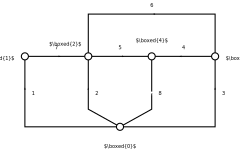
\includegraphics{Imatges/Cap-ResXarxElec-Exemple-Graf.pdf}
\end{minipage}
\hfill
\begin{minipage}[c]{9cm}
   \[
   \boldsymbol{A} = \left( \begin{array}{rrrrrrrr}
     -1 & 0 & 0 & 0 & 0 & 0 & 1 & 0 \\
     0 & -1 & 0 & 0 & 1 & 1 & -1 & 0 \\
     0 & 0 & -1 & 1 & 0 & -1 & 0 & 0 \\
     0 & 0 & 0 & -1 & -1 & 0 & 0 & 1
   \end{array}\right)
   \]
\end{minipage}
\hfill{}
\end{figure}

Formem a continuaci\'{o} la matriu $\mcmplx{Z}\ped{B}$ i els vectors $\mcmplx{J}\ped{B}'$ i $\mcmplx{E}\ped{B}'$ (tots els valors en p.u.):
\[
   \mcmplx{Z}\ped{B} = \ju \cdot
   \begin{pmatrix}
     0{,}25 & 0 & 0 & 0 & 0 & 0 & 0 & 0 \\
     0 & 0{,}20 & 0 & 0 & 0 & 0 & 0 & 0 \\
     0 & 0 & 0{,}25 & 0 & 0 & 0 & 0 & 0 \\
     0 & 0 & 0 & 0{,}10 & 0 & 0 & 0 & 0 \\
     0 & 0 & 0 & 0 & 0{,}405 & 0{,}05 & 0 & 0 \\
     0 & 0 & 0 & 0 & 0{,}05 & 0{,}50 & 0 & 0 \\
     0 & 0 & 0 & 0 & 0 & 0 & 0{,}16 & 0 \\
     0 & 0 & 0 & 0 & 0 & 0 & 0 & -25
   \end{pmatrix}
   \;\;
   \mcmplx{J}\ped{B}' =
   \begin{pmatrix}
    0 \\
    0 \\
    0 \\
    0 \\
    0 \\
    0 \\
    0 \\
    2 - \ju 0{,}9
   \end{pmatrix}
   \;\;
   \mcmplx{E}\ped{B}' =
   \begin{pmatrix}
    1{,}1 \\
    1{,}05 + \ju 0{,}10 \\
    1{,}08 + \ju 0{,}12 \\
    0 \\
    0 \\
    0 \\
    0 \\
    0
   \end{pmatrix}
\]

Calculem ara la matriu $\mcmplx{Y}\ped{B}=\mcmplx{Z}\ped{B}^{-1}$ i el vector $\mcmplx{J}\ped{B} = \mcmplx{J}\ped{B}' + \mcmplx{Y}\ped{B} \,\mcmplx{E}\ped{B}'$  (tots els valors en p.u.):
\[
   \mcmplx{Y}\ped{B} = \ju \cdot
   \begin{pmatrix}
     -4 & 0 & 0 & 0 & 0 & 0 & 0 & 0 \\
     0 & -5 & 0 & 0 & 0 & 0 & 0 & 0 \\
     0 & 0 & -4 & 0 & 0 & 0 & 0 & 0 \\
     0 & 0 & 0 & -10 & 0 & 0 & 0 & 0 \\
     0 & 0 & 0 & 0 & -2{,}5 & 0{,}25 & 0 & 0 \\
     0 & 0 & 0 & 0 & 0{,}25 & -2{,}025 & 0 & 0 \\
     0 & 0 & 0 & 0 & 0 & 0 & -6{,}25 & 0 \\
     0 & 0 & 0 & 0 & 0 & 0 & 0 & 0{,}04
   \end{pmatrix}
   \qquad
   \mcmplx{J}\ped{B} =
   \begin{pmatrix}
    -\ju 4{,}4 \\
    0{,}5 - \ju 5{,}25 \\
    0{,}48 - \ju 4{,}32 \\
    0 \\
    0 \\
    0 \\
    0 \\
    2 - \ju 0{,}9
   \end{pmatrix}
\]

Continuem amb el c\`{a}lcul de la matriu $\mcmplx{Y}\ped{N} =
\boldsymbol{A} \mcmplx{Y}\ped{B} \transp{\boldsymbol{A}}$ i dels
vectors $\mcmplx{J}\ped{N} = - \boldsymbol{A} \mcmplx{J}\ped{B}$ i
$\mcmplx{V}\ped{N} = \mcmplx{Y}\ped{N}^{-1} \mcmplx{J}\ped{N}$ (tots
els valors en p.u.):
\[
   \mcmplx{Y}\ped{N} = \ju \cdot
   \begin{pmatrix}
     -10{,}25 & 6{,}25 & 0 & 0 \\
     6{,}25 & -15{,}275 & 1{,}775 & 2{,}25 \\
     0 & 1{,}775 & -16{,}025 & 10{,}25 \\
     0 & 2{,}25 & 10{,}25 & -12{,}46
   \end{pmatrix}
   \;\;
   \mcmplx{J}\ped{N} =
   \begin{pmatrix}
    -\ju 4{,}4 \\
    0{,}5 - \ju 5{,}25 \\
    0{,}48 - \ju 4{,}32 \\
    -2 + \ju 0{,}9
   \end{pmatrix}
   \;\;
   \mcmplx{V}\ped{N} =
   \left(\begin{array}{l}
    1{,}0494_{\angle -1{,}4909\degree} \\
    1{,}0175_{\angle -2{,}5224\degree} \\
    0{,}9727_{\angle -10{,}3558\degree} \\
    0{,}9512_{\angle -19{,}1752\degree}
   \end{array}\right)
\]

Finalment, calculem les tensions i els corrents de les branques,
mitjan\c{c}ant els vectors $\mcmplx{U}\ped{B} = \transp{\boldsymbol{A}}
\mcmplx{V}\ped{N}$ i $\mcmplx{I}\ped{B} =  \mcmplx{Y}\ped{B}\,
\mcmplx{U}\ped{B} + \mcmplx{J}\ped{B}$ (tots els valors en p.u.):
\[
   \mcmplx{U}\ped{B} =
   \left(\begin{array}{l}
     1{,}0494_{\angle 178{,}5091\degree} \\
     1{,}0175_{\angle 177{,}4776\degree} \\
     0{,}9727_{\angle 169{,}6442\degree} \\
     0{,}1495_{\angle 67{,}0039\degree} \\
     0{,}2925_{\angle 66{,}2049\degree} \\
     0{,}1431_{\angle 65{,}3702\degree} \\
     0{,}0370_{\angle 28{,}1937\degree} \\
     0{,}9512_{\angle -19{,}1752\degree}
   \end{array}\right)
   \qquad
   \mcmplx{I}\ped{B} =
   \left(\begin{array}{l}
     0{,}2312_{\angle -61{,}8063\degree} \\
     0{,}7431_{\angle -13{,}0406\degree} \\
     1{,}2782_{\angle -22{,}6715\degree} \\
     1{,}4946_{\angle -22{,}9961\degree} \\
     0{,}6955_{\angle -23{,}7522\degree} \\
     0{,}2166_{\angle -24{,}9115\degree} \\
     0{,}2312_{\angle -61{,}8063\degree} \\
     2{,}1901_{\angle -23{,}2362\degree}
   \end{array}\right)
\]

Calcularem ara la pot\`{e}ncia cedida pels tres generadors G1, G2 i G3, i la pot\`{e}ncia absorbida per la c\`{a}rrega Q8. Cal tenir en compte que per calcular les pot\`{e}ncies cedides per generadors, els vectors que representen la for\c{c}a electromotriu del generador i el corrent que travessa el generador han de tenir el mateix sentit de refer\`{e}ncia; aix\'{\i} mateix, per calcular les pot\`{e}ncies absorbides per c\`{a}rregues, els vectors que representen la caiguda de tensi\'{o} a la c\`{a}rrega i el corrent que travessa la c\`{a}rrega han de tenir el mateix sentit de refer\`{e}ncia. Amb aquestes consideracions, tenim:
\begin{alignat*}{3}
   \cmplx{s}\ped{G1} &= \cmplx{e}\ped{1} \, \mcmplx{I}\ped{B}^*(1) &&= 1{,}1 \cdot
    0{,}2312_{\angle 61{,}8063\degree} &&= 0{,}1201 + \ju 0{,}2241 \unit{p.u.} \\
   \cmplx{s}\ped{G2} &= \cmplx{e}\ped{2} \, \mcmplx{I}\ped{B}^*(2) &&=
   (1{,}05 + \ju 0{,}10) \cdot 0{,}7431_{\angle 13{,}0406\degree} &&=
   0{,}7433 + \ju 0{,}2484\unit{p.u.}   \\
   \cmplx{s}\ped{G3} &= \cmplx{e}\ped{3} \, \mcmplx{I}\ped{B}^*(3) &&=
   (1{,}08 + \ju 0{,}12) \cdot 1{,}2782_{\angle 22{,}6715\degree} &&=
   1{,}2146 + \ju 0{,}6736\unit{p.u.}   \\
   \cmplx{s}\ped{Q8} &= \mcmplx{U}\ped{B}(8) \, \mcmplx{I}\ped{B}^*(8) &&=
   0{,}9512_{\angle -19{,}1752\degree} \cdot 2{,}1901_{\angle          23{,}2362\degree}     &&= 2{,}0780 + \ju 0{,}1475\unit{p.u.}
\end{alignat*}

La difer\`{e}ncia entre les pot\`{e}ncies generades i la pot\`{e}ncia absorbida, \'{e}s la pot\`{e}ncia perduda en la resta de components de la xarxa:
\[
   \cmplx{s}\ped{G1} + \cmplx{s}\ped{G2} + \cmplx{s}\ped{G3} -
   \cmplx{s}\ped{Q8} = \ju 0{,}9986\unit{p.u.}
\]
\end{exemple}


\section{M\`{e}tode particular de resoluci\'{o} sense acoblaments magn\`{e}tics}
\index{metode@m\`{e}tode dels nusos!cas particular!sense acoblaments
magn\`{e}tics}

Quan no hi ha acoblaments magn\`{e}tics entre branques de la xarxa, la matriu $\mcmplx{Y}\ped{N}\{n \times n\}$ i el vector $\mcmplx{J}\ped{N}\{n\}$ es poden formar de manera directa, a partir dels components de la xarxa i del seu graf orientat associat.

Per ajudar-nos en l'explicaci\'{o} d'aquest m\`{e}tode simplificat, farem \'{u}s
del mateix exemple de la Figura \vref{pic:metode_nusos}, per\`{o}
suposant que no hi ha acoblament magn\`{e}tic entre les branques 2 i 3
($\cmplx{X}\ped{M}=0$).

La matriu $\mcmplx{Y}\ped{N}\{n \times n\}$ i el vector $\mcmplx{J}\ped{N}\{n\}$ es formen tal com es descriu a continuaci\'{o}:

\begin{list}{}
   {\setlength{\labelwidth}{20mm} \setlength{\leftmargin}{22mm} \setlength{\labelsep}{2mm}}

   \item[$\mcmplx{Y}\ped{N}\{n \times n\}$:] \index{matriu!d'admit\`{a}ncies de nus $\mcmplx{Y}\ped{N}$}Matriu d'admit\`{a}ncies de nus. Els elements de la diagonal estan formats per la suma de les admit\`{a}ncies de les branques que incideixen en cada nus.
   Els elements de fora de la diagonal estan formats per la suma, canviada de signe, de les admit\`{a}ncies de les branques que estan connectades entre cada parella de nusos.

   En el nostre exemple tenim:
   \[
      \mcmplx{Y}\ped{N} =
      \begin{pmatrix}
            \frac{1}{20} + \frac{1}{\ju 20} +  \frac{1}{10} &
            -\left[\frac{1}{20} + \frac{1}{\ju 20}\right] \\
            -\left[\frac{1}{20} + \frac{1}{\ju 20}\right]  &
            \frac{1}{20} + \frac{1}{\ju 20} +  \frac{1}{\ju 5} + \frac{1}{10}
      \end{pmatrix} =
      \frac{1}{20} \cdot \begin{pmatrix}
            3 - \ju  & -1 + \ju \\ -1 + \ju & 3 - \ju 5
      \end{pmatrix}\unit{S}
   \]

   \item[$\mcmplx{J}\ped{N}\{n\}$:] \index{vector!d'intensivitats de nus $\mcmplx{J}\ped{N}$}Vector
d'intensivitats de nus. Cada element d'aquest vector est\`{a} format per la suma de
les intensivitats, degudes a les fonts de corrent i a les fonts de tensi\'{o}, de les
branques que incideixen en cada nus; el signe de cada intensivitat \'{e}s positiu si el
corrent va cap al nus, i negatiu si se n'allunya. Les fonts de tensi\'{o} han de
transformar-se en fonts de corrent, utilitzant l'equaci\'{o} \eqref{eq:Thevenin-Norton} de
la p\`{a}gina \pageref{eq:Thevenin-Norton}.

   En el nostre exemple tenim:
   \[
      \mcmplx{J}\ped{N} =
      \begin{pmatrix}
            \frac{50}{\ju 20} +  \frac{200}{10} \\
            - \frac{50}{\ju 20} + 4
      \end{pmatrix} =
      \frac{1}{2} \cdot \begin{pmatrix}
            40 - \ju 5 \\
            8 + \ju 5
      \end{pmatrix}\unit{A}
   \]

\end{list}

\index{vector!de potencials de nus $\mcmplx{V}\ped{N}$}Finalment,
trobem el vector de potencials de nus $\mcmplx{V}\ped{N}\{n\}$, tal
com  hem fet en l'apartat anterior, aplicant l'equaci\'{o} \eqref{eq:vn}

En el nostre exemple tenim:
\[
   \mcmplx{V}\ped{N} =
   20 \cdot \begin{pmatrix}
         3 - \ju  & -1 + \ju \\ -1 + \ju & 3 - \ju 5
   \end{pmatrix} ^{-1} \cdot
   \frac{1}{2} \cdot \begin{pmatrix}
         40 - \ju 5 \\
         8 + \ju 5
   \end{pmatrix} =
   \frac{1}{17} \cdot \begin{pmatrix}
         2450 + \ju 535 \\ 540  + \ju 545
   \end{pmatrix}\unit{V}
\]

Si volem trobar ara de forma sistem\`{a}tica, totes les tensions i tots
els corrents i  de les branques de la xarxa, haurem d'utilitzar
l'equaci\'{o} \eqref{eq:ur} de la p\`{a}gina \pageref{eq:ur} i l'equaci\'{o}
\eqref{eq:ir} de la p\`{a}gina \pageref{eq:ir}; aix\`{o} vol dir que haurem
de formar les matrius $\boldsymbol{A}$ i $\mcmplx{Y}\ped{B}$ i el
vector $\mcmplx{J}\ped{B}$. No obstant, si \'{u}nicament estem
interessats en algun corrent o en alguna tensi\'{o} de branca, podem
resoldre el problema aplicant les lleis de Kirchhoff a les branques
que ens interessin.


\begin{exemple}
A partir del circuit de la Figura \vref{pic:metode_nusos}, amb
$\cmplx{X}\ped{M}=0$, es tracta de trobar els corrents que circulen
per les branques 2 i 5.

Partint dels potencials dels nusos 1 i 2 calculats anteriorment, i
aplicant les lleis de Kirchhoff a les branques 2 i 5 tenim:
\begin{align*}
   \cmplx{I}_2 &= \frac{-\cmplx{E}_2 + [\mcmplx{V}\ped{N}(1) - \mcmplx{V}\ped{N}(2)]}
                  {\cmplx{X}_2} = \frac{-50 + \frac{2450+\ju 535 -540
                  - \ju 545}{17}} {\ju 20} = \frac{-1 - \ju 106}{34}\unit{A} \\[1.5ex]
   \cmplx{I}_5 &=  \frac{- \mcmplx{V}\ped{N}(2)}{R_5}  + \cmplx{J}_5 =
                  \frac{\frac{-540 - \ju 545}{17}}{10} + 4 =
                  \frac{28 - \ju 109}{34}\unit{A}
\end{align*}

\end{exemple}

\section{M\`{e}tode particular de resoluci\'{o} amb acoblaments magn\`{e}tics}
\index{metode@m\`{e}tode dels nusos!cas particular!amb acoblaments
magn\`{e}tics}

Quan hi ha acoblaments magn\`{e}tics entre branques de la xarxa que no
tenen cap font de tensi\'{o} o de corrent, tamb\'{e} es pot aplicar el
m\`{e}tode de resoluci\'{o} descrit en l'apartat anterior, substituint
pr\`{e}viament les dues branques acoblades per un circuit equivalent
d'admit\`{a}ncies, segons es veur\`{a} a continuaci\'{o}.

Un cop obtingut el circuit equivalent de les dues branques acoblades
magn\`{e}ticament, ja es pot formar la matriu $\mcmplx{Y}\ped{N}\{n \times n\}$ i
el vector $\mcmplx{J}\ped{N}\{n\}$, i  resoldre la xarxa, tal com s'ha fet en
l'apartat anterior.

En la Figura \vref{pic:equiv_acobl} es pot veure aquest circuit
equivalent.
\begin{figure}[htb]
\centering
    
\includegraphics{Imatges/Cap-ResXarxElec-Acoblament.pdf}
   \caption{Circuit equivalent de dues branques acoblades magn\`{e}ticament} \label{pic:equiv_acobl}
\end{figure}

Els valors de les admit\`{a}ncies d'aquest circuit equivalent
s\'{o}n:\index{acoblament magn\`{e}tic!circuit equivalent}

\parbox{15cm}
{ \begin{align*}
   \cmplx{Y}_{\alphaup\betaup} &= \frac{\cmplx{Z}_{\gammaup\deltaup}}{\cmplx{Z}_{\alphaup\betaup}\, \cmplx{Z}_{\gammaup\deltaup}-\cmplx{X}\ped{M}^2} &
   \cmplx{Y}_{\alphaup\gammaup} &= \cmplx{Y}_{\betaup\deltaup} = \frac{\cmplx{X}\ped{M}}{\cmplx{Z}_{\alphaup\betaup}\, \cmplx{Z}_{\gammaup\deltaup}-\cmplx{X}\ped{M}^2} \\[1.5ex]
   \cmplx{Y}_{\gammaup\deltaup} &= \frac{\cmplx{Z}_{\alphaup\betaup}}{\cmplx{Z}_{\alphaup\betaup}\, \cmplx{Z}_{\gammaup\deltaup}-\cmplx{X}\ped{M}^2} &
   \cmplx{Y}_{\alphaup\deltaup} &= \cmplx{Y}_{\gammaup\betaup} = \frac{-\cmplx{X}\ped{M}}{\cmplx{Z}_{\alphaup\betaup}\, \cmplx{Z}_{\gammaup\deltaup}-\cmplx{X}\ped{M}^2}
\end{align*} }
\hfill
\parbox{1cm}{\begin{align}\end{align}}

Un cop hem resolt la xarxa i hem trobat els potencials dels quatre
nusos $\mcmplx{V}\ped{N}(\alphaup)$, $\mcmplx{V}\ped{N}(\betaup)$,
$\mcmplx{V}\ped{N}(\gammaup)$ i $\mcmplx{V}\ped{N}(\deltaup)$, podem
trobar els dos corrents $\cmplx{I}_{\alphaup\betaup}$ i
$\cmplx{I}_{\gammaup\deltaup}$, a partir de les expressions seg\"{u}ents:
\begin{subequations}
\begin{align}
    \cmplx{I}_{\alphaup\betaup} &=  \frac{[\mcmplx{V}\ped{N}(\alphaup) - \mcmplx{V}\ped{N}(\betaup)] \, \cmplx{Z}_{\gammaup\deltaup} - [\mcmplx{V}\ped{N}(\gammaup) - \mcmplx{V}\ped{N}(\deltaup)] \,
    \cmplx{X}\ped{M}}{\cmplx{Z}_{\alphaup\betaup}\,
    \cmplx{Z}_{\gammaup\deltaup}-\cmplx{X}\ped{M}^2} \label{eq:i_ab}
    \\[1.5ex]
    \cmplx{I}_{\gammaup\deltaup} &= \frac{[\mcmplx{V}\ped{N}(\gammaup) - \mcmplx{V}\ped{N}(\deltaup)] \, \cmplx{Z}_{\alphaup\betaup} - [\mcmplx{V}\ped{N}(\alphaup) - \mcmplx{V}\ped{N}(\betaup)] \,
    \cmplx{X}\ped{M}}{\cmplx{Z}_{\alphaup\betaup}\,
    \cmplx{Z}_{\gammaup\deltaup}-\cmplx{X}\ped{M}^2} \label{eq:i_gd}
\end{align}
\end{subequations}

El cas que hem vist fins ara, \'{e}s el m\'{e}s general de tots els
possibles, ja que suposa que els quatre nusos $\alphaup$, $\betaup$,
$\gammaup$ i $\deltaup$ s\'{o}n diferents entre si. Es pot presentar el cas,
no obstant, on dos nusos siguin en realitat el mateix, en tenir les
dues branques acoblades magn\`{e}ticament, un extrem connectat al mateix
nus; en aquest cas el circuit equivalent resultant es pot derivar
del corresponent al cas general de forma senzilla.

Si suposem, per exemple, que les dues branques de la Figura
\vref{pic:equiv_acobl} estiguessin unides pels extrems de la dreta,
\'{e}s a dir $\betaup\equiv\deltaup$, en aquest cas l'admit\`{a}ncia entre
$\alphaup$ i $\gammaup$ seria $\cmplx{Y}_{\alphaup\gammaup}$, l'admit\`{a}ncia
entre $\betaup$ i $\deltaup$ desapareixeria, l'admit\`{a}ncia entre $\alphaup$
i $\betaup$ seria $\cmplx{Y}_{\alphaup\betaup} +
\cmplx{Y}_{\alphaup\deltaup}$, i finalment, l'admit\`{a}ncia entre $\gammaup$
i $\betaup$ seria $\cmplx{Y}_{\gammaup\betaup} +
\cmplx{Y}_{\gammaup\deltaup}$. Els corrents $\cmplx{I}_{\alphaup\betaup}$ i
$\cmplx{I}_{\gammaup\deltaup}$, es calcularien tamb\'{e} amb les equacions
\eqref{eq:i_ab} i \eqref{eq:i_gd}, tenint en compte que
$\mcmplx{V}\ped{N}(\betaup)\equiv\mcmplx{V}\ped{N}(\deltaup)$.

\section{Circuits equivalents Th\'{e}venin i Norton} \index{teorema!de Th\'{e}venin} \index{teorema!de Norton} \index{metode@m\`{e}tode dels nusos!circuits equivalents Th\'{e}venin i Norton}\label{sec:xarxes_Zth}

\index{matriu!d'imped\`{a}ncies de nus $\mcmplx{Z}\ped{N}$}Per trobar el
circuit equivalent Th\'{e}venin o Norton entre dos nusos qualssevol
d'una xarxa, ens cal el vector de potencials de nus
$\mcmplx{V}\ped{N}\{n\}$, obtingut segons s'ha descrit en els
apartats anteriors, i la matriu d'imped\`{a}ncies de nus
$\mcmplx{Z}\ped{N}\{n\times n\}$; aquesta matriu est\`{a} definida per
la relaci\'{o} seg\"{u}ent:
\begin{equation}
   \mcmplx{Z}\ped{N} = \mcmplx{Y}\ped{N}^{-1}
\end{equation}

A partir del vector $\mcmplx{V}\ped{N}$ i de la matriu
$\mcmplx{Z}\ped{N}$, podem trobar la font de tensi\'{o} i la imped\`{a}ncia
Th\'{e}venin equivalents entre dos nusos qualssevol.

La tensi\'{o} Th\'{e}venin $\cmplx{E}\ped{Th}^{(\alphaup,0)}$ i la imped\`{a}ncia
Th\'{e}venin $\cmplx{Z}\ped{Th}^{(\alphaup,0)}$, entre  un nus qualsevol
$\alphaup$ i el nus de refer\`{e}ncia 0, s'obtenen amb les equacions
seg\"{u}ents:
\begin{align}
    \cmplx{E}\ped{Th}^{(\alphaup,0)} &= \mcmplx{V}\ped{N}(\alphaup) \\
    \cmplx{Z}\ped{Th}^{(\alphaup,0)} &= \mcmplx{Z}\ped{N}(\alphaup,\alphaup)
\end{align}

La tensi\'{o} Th\'{e}venin $\cmplx{E}\ped{Th}^{(\alphaup,\betaup)}$ i la
imped\`{a}ncia Th\'{e}venin $\cmplx{Z}\ped{Th}^{(\alphaup,\betaup)}$, entre dos
nusos qualssevol $\alphaup$ i $\betaup$, s'obtenen amb les equacions
seg\"{u}ents:
\begin{align}
    \cmplx{E}\ped{Th}^{(\alphaup,\betaup)} &= \mcmplx{V}\ped{N}(\alphaup) - \mcmplx{V}\ped{N}(\betaup) \\
    \cmplx{Z}\ped{Th}^{(\alphaup,\betaup)} &= \mcmplx{Z}\ped{N}(\alphaup,\alphaup) +
    \mcmplx{Z}\ped{N}(\betaup,\betaup) - \mcmplx{Z}\ped{N}(\alphaup,\betaup) -
    \mcmplx{Z}\ped{N}(\betaup,\alphaup)
\end{align}

A partir d'aquests valors podem calcular els valors del circuit Norton equivalent, utilitzant l'equaci\'{o} \eqref{eq:Thevenin-Norton} de la p\`{a}gina \pageref{eq:Thevenin-Norton}.


\begin{exemple}
Continuant amb el circuit de la Figura \vref{pic:metode_nusos}, es
tracta de trobar els circuits Th\'{e}venin i Norton equivalents de la
xarxa, entre els nusos 1 i 2.

El vector $\mcmplx{V}\ped{N}$ \'{e}s el calculat a la p\`{a}gina \pageref{eq:vn_exemp}.

Trobem a continuaci\'{o} la matriu $\mcmplx{Z}\ped{N}$, a partir de la matriu $\mcmplx{Y}\ped{N}$
calculada a la p\`{a}gina \pageref{eq:yn}:
\[
   \mcmplx{Z}\ped{N} =
   60 \cdot \begin{pmatrix}
            9 - \ju 4 & -3 + \ju 8 \\
            3 + \ju 8 & 9 - \ju 28
      \end{pmatrix} ^{-1} =
   \frac{1}{202} \cdot \begin{pmatrix}
         1445 + \ju 310 & 415 + \ju 110 \\
         415 + \ju 110 & 245 + \ju 430
   \end{pmatrix}\unit{\ohm}
\]

Els valors del circuit Th\'{e}venin equivalent que busquem s\'{o}n:
\begin{align*}
   \cmplx{E}\ped{Th}^{(1,2)} &= \frac{15430 + \ju 2295}{101} - \frac{3390 + \ju 2085}{101} =
   \frac{12040 + \ju 210}{101}\unit{V} \\[2ex]
   \cmplx{Z}\ped{Th}^{(1,2)} &= \frac{1445 + \ju 310}{202} + \frac{245 + \ju 430}{202} -
   2\cdot\frac{415 + \ju 110}{202} = \frac{430 + \ju 260}{101}\unit{\ohm}
\end{align*}

Els valors del circuit Norton equivalent que busquem s\'{o}n:
\begin{align*}
   \cmplx{J}\ped{No}^{(1,2)} &= \frac{\cmplx{E}\ped{Th}^{(1,2)}}{\cmplx{Z}\ped{Th}^{(1,2)}} =
   \frac{\frac{12040 + \ju 210}{101}\unit{V}}{\frac{430 + \ju 260}{101}\unit{\ohm}} =
   \frac{518 - \ju 301}{25}\unit{A} \\[2ex]
   \cmplx{Y}\ped{No}^{(1,2)} &= \frac{1}{\cmplx{Z}\ped{Th}^{(1,2)}} =
   \frac{1}{\frac{430 + \ju 260}{101}\unit{\ohm}} = \frac{43 - \ju 26}{250}\unit{S}
\end{align*}

\end{exemple}

      \chapter{Flux de C\`{a}rregues}
\index{flux de c\`{a}rregues}\label{chap:flux_carregues}

Es tracta en aquest cap\'{\i}tol el m\`{e}tode de resoluci\'{o} del problema del flux de c\`{a}rregues en
sistemes el\`{e}ctrics de pot\`{e}ncia.

\section{Introducci\'{o}}

Quan les dades que es coneixen de les c\`{a}rregues d'una xarxa no s\'{o}n
les seves imped\`{a}ncies o admit\`{a}ncies, sin\'{o} les pot\`{e}ncies que
absorbeixen, no podem emprar el m\`{e}tode dels nusos, descrit en el
Cap\'{\i}tol \ref{chap:nusos}, per tal de resoldre la xarxa.

En aquest cas, el m\`{e}tode de resoluci\'{o} es basa en escriure per a cada
nus les equacions pertinents del balan\c{c} de pot\`{e}ncia activa i
reactiva, i resoldre-les. La soluci\'{o} del sistema d'equacions
resultant, ens proporcionar\`{a} les tensions de tots els nusos de la
xarxa, i el flux de pot\`{e}ncia activa i reactiva entre els seus nusos.

El sistema d'equacions que cal resoldre \'{e}s no lineal, i per tant,
cal emprar algun m\`{e}tode num\`{e}ric per a la seva resoluci\'{o}, com ara el
de Newton-Raphson;\index{Newton-Raphson} aqu\'{\i}, no obstant, no
s'explicar\`{a} cap m\`{e}tode num\`{e}ric de resoluci\'{o} de sistemes d'equacions
no lineals, ja que aix\`{o} cau fora de l'abast d'aquest llibre. Aix\`{o}
per\`{o}, no hauria de suposar cap problema, ja que avui dia aquests
sistemes d'equacions es poden resoldre f\`{a}cilment amb programes
d'ordinador de c\`{a}lcul matem\`{a}tic, com ara els programes
\textit{Mathematica}${}^\circledR$ o \textit{MATLAB}${}^\circledR$,
\index{Mathematica@\textit{Mathematica}${}^\circledR$}
\index{MATLAB@\textit{MATLAB}${}^\circledR$} o amb calculadores
cient\'{\i}fiques, com ara la calculadora \textsf{HP-49G}.

\section{Models matem\`{a}tics} \index{flux de c\`{a}rregues!models matem\`{a}tics}

En els estudis de flux de c\`{a}rregues, els elements que es consideren s\'{o}n:
\begin{dinglist}{'167}
   \item C\`{a}rregues
   \item L\'{\i}nies el\`{e}ctriques
   \item Transformadors amb regulaci\'{o} variable (amb decalatge o sense)
\end{dinglist}

\subsection{C\`{a}rregues}

Les c\`{a}rregues v\'{e}nen sempre definides per la pot\`{e}ncia que absorbeixen, \'{e}s a dir, es consideren fonts de pot\`{e}ncia constant.

\subsection{L\'{\i}nies el\`{e}ctriques} \index{linies@l\'{\i}nies el\`{e}ctriques}

Les l\'{\i}nies el\`{e}ctriques es modelen mitjan\c{c}ant un circuit equivalent
per fase en {"<}$\piup${">}, format per una imped\`{a}ncia longitudinal i dues
admit\`{a}ncies transversals, tal com es pot veure en la Figura
\vref{pic:equiv_linia}. En aquesta figura s'ha suposat que la l\'{\i}nia
est\`{a} connectada entre els nusos 1 i 2; les admit\`{a}ncies transversals,
tenen sempre un extrem connectat a terra (nus 0 de refer\`{e}ncia).
\index{linies@l\'{\i}nies el\`{e}ctriques!circuit equivalent en
\guillemotleft$\piup$\guillemotright}

\begin{figure}[htb]
\centering
    \includegraphics{Imatges/Cap-FluxCarregues-Linia.pdf}
\caption{Circuit equivalent d'una l\'{\i}nia el\`{e}ctrica}
\label{pic:equiv_linia}
\end{figure}

A partir dels par\`{a}metres propis d'una l\'{\i}nia: la seva imped\`{a}ncia
longitudinal  total per fase $\cmplx{Z}\ped{t}$ i la seva admit\`{a}ncia
transversal total per fase $\cmplx{Y}\ped{t}$, definim la imped\`{a}ncia
caracter\'{\i}stica $\cmplx{Z}\ped{c}$ i l'angle caracter\'{\i}stic
$\cmplx{\theta}\ped{c}$ de la l\'{\i}nia: \index{linies@l\'{\i}nies
el\`{e}ctriques!imped\`{a}ncia caracter\'{\i}stica} \index{linies@l\'{\i}nies
el\`{e}ctriques!angle caracter\'{\i}stic} \index{Zc@$\cmplx{Z}\ped{c}$}
\index{$\cmplx{\theta}\ped{c}$}
\begin{equation}
   \cmplx{Z}\ped{c} = \sqrt{\frac{\cmplx{Z}\ped{t}}{\cmplx{Y}\ped{t}}} \qquad \qquad
   \cmplx{\theta}\ped{c} = \sqrt{\cmplx{Z}\ped{t} \,\cmplx{Y}\ped{t} }
\end{equation}

Amb aquest dos par\`{a}metres, les equacions hiperb\`{o}liques de
transmissi\'{o} d'una l\'{\i}nia s\'{o}n: \index{linies@l\'{\i}nies
el\`{e}ctriques!equacions hiperb\`{o}liques de transmissi\'{o}}
\begin{equation}\label{eq:linia_eq_trans}
   \cmplx{U}_1 = \cmplx{U}_2 \cosh \cmplx{\theta}\ped{c}  + \cmplx{I}_2 \,\cmplx{Z}\ped{c} \sinh \cmplx{\theta}\ped{c}   \qquad \qquad
   \cmplx{I}_1 = \cmplx{U}_2 \, \frac{\sinh \cmplx{\theta}\ped{c}}{\cmplx{Z}\ped{c}}  +   \cmplx{I}_2 \cosh \cmplx{\theta}\ped{c}
\end{equation}

D'altra banda, en el circuit de la Figura \vref{pic:equiv_linia} es compleix:
\begin{equation}\label{eq:linia_eq}
   \cmplx{I}_2 = \frac{\cmplx{U}_1 - \cmplx{U}_2}{\cmplx{Z}_\piup} - \cmplx{Y}_\piup\, \cmplx{U}_2
   \qquad \qquad
   \cmplx{U}_1 = (1 + \cmplx{Z}_\piup\,\cmplx{Y}_\piup ) \cmplx{U}_2 + \cmplx{Z}_\piup\,\cmplx{I}_2
\end{equation}

Identificant entre si els termes de les equacions
\eqref{eq:linia_eq_trans} i \eqref{eq:linia_eq}, obtenim els
par\`{a}metres del circuit equivalent de la l\'{\i}nia.
\begin{alignat}{2}
   \cmplx{Z}_\piup &= \cmplx{Z}\ped{c} \sinh \cmplx{\theta}\ped{c} &&= \cmplx{Z}\ped{t} \,
   \frac{\sinh \cmplx{\theta}\ped{c}}{\cmplx{\theta}\ped{c}} \\[1.5ex]
   \cmplx{Y}_\piup &= \frac{\tanh (\cmplx{\theta}\ped{c} / 2) }{\cmplx{Z}\ped{c}} &&=
   \frac{\cmplx{Y}\ped{t}}{2} \, \frac{\tanh (\cmplx{\theta}\ped{c} / 2)}{\cmplx{\theta}\ped{c} / 2}
\end{alignat}

Ara b\'{e}, en la majoria dels casos es compleix: $|\cmplx{\theta}\ped{c}| \ll 1$, i utilitzant els desenvolupaments en s\`{e}rie de les funcions $\sinh$ i $\tanh$, al voltant de 0, tenim:
\begin{align}
   \cmplx{Z}_\piup &= \cmplx{Z}\ped{t} \, \left[ 1 + \frac{\cmplx{\theta}\ped{c}^2}{3!} +
   \frac{\cmplx{\theta}\ped{c}^4}{5!} + \cdots \right] \approx \cmplx{Z}\ped{t} \\[1.5ex]
   \cmplx{Y}_\piup &= \frac{\cmplx{Y}\ped{t}}{2} \,\left[ 1 - \frac{(\cmplx{\theta}\ped{c}/2)^2}{3} + \frac{2 (\cmplx{\theta}\ped{c}/2)^4}{15} - \cdots \right] \approx \frac{\cmplx{Y}\ped{t}}{2}
\end{align}

Utilitzant aquests valors, la contribuci\'{o} d'una l\'{\i}nia el\`{e}ctrica, a
la matriu d'admit\`{a}ncies de nus $\mcmplx{Y}\ped{N}$ de la xarxa a la
qual pertany, \'{e}s: \index{linies@l\'{\i}nies el\`{e}ctriques!matriu
d'admit\`{a}ncies de nus $\mcmplx{Y}\ped{N}$}
\index{matriu!d'admit\`{a}ncies de nus $\mcmplx{Y}\ped{N}$}
\begin{equation}
   \mcmplx{Y}\ped{N} = \begin{pmatrix}
     \dfrac{\cmplx{Y}\ped{t}}{2} + \dfrac{1}{\cmplx{Z}\ped{t}} & -\dfrac{1}{\cmplx{Z}\ped{t}}\\[2.5ex]
     -\dfrac{1}{\cmplx{Z}\ped{t}} & \dfrac{\cmplx{Y}\ped{t}}{2} + \dfrac{1}{\cmplx{Z}\ped{t}}
   \end{pmatrix}
\end{equation}

Els fluxos de pot\`{e}ncia a trav\'{e}s de la l\'{\i}nia, $\cmplx{S}_{12}$ (del
nus 1 al 2), i $\cmplx{S}_{21}$ (del nus 2 a l'1), v\'{e}nen donats per
les expressions:\index{linies@l\'{\i}nies el\`{e}ctriques!fluxos de pot\`{e}ncia}
\begin{align}
   \cmplx{S}_{12} &= \cmplx{U}_1 \left[ \left( \frac{\cmplx{Y}\ped{t}}{2} + \frac{1}{\cmplx{Z}\ped{t}} \right) \cmplx{U}_1 - \frac{1}{\cmplx{Z}\ped{t}} \cmplx{U}_2 \right]^* = \cmplx{U}_1 \left[ \frac{\cmplx{Y}\ped{t}}{2}\, \cmplx{U}_1 + \frac{\cmplx{U}_1 - \cmplx{U}_2}{\cmplx{Z}\ped{t}} \right]^* \label{eq:lin_s12}
   \\[1.5ex]
   \cmplx{S}_{21} &= \cmplx{U}_2 \left[ \left( \frac{\cmplx{Y}\ped{t}}{2} + \frac{1}{\cmplx{Z}\ped{t}} \right) \cmplx{U}_2 - \frac{1}{\cmplx{Z}\ped{t}} \cmplx{U}_1 \right]^* = \cmplx{U}_2 \left[ \frac{\cmplx{Y}\ped{t}}{2} \,\cmplx{U}_2 + \frac{\cmplx{U}_2 - \cmplx{U}_1}{\cmplx{Z}\ped{t}} \right]^* \label{eq:lin_s21}
\end{align}

Finalment, les p\`{e}rdues de transmissi\'{o} en la  l\'{\i}nia
$\Delta\cmplx{S}$, v\'{e}nen donades per
l'expressi\'{o}:\index{linies@l\'{\i}nies el\`{e}ctriques!p\`{e}rdues de transmissi\'{o}}
\begin{equation}
   \Delta\cmplx{S} = \cmplx{S}_{12} + \cmplx{S}_{21} = \left[ \frac{\cmplx{Y}\ped{t}}{2} + \frac{1}{\cmplx{Z}\ped{t}} \right]^* \Big[ |\cmplx{U}_1|^2 + |\cmplx{U}_2|^2 \Big] - 2 \, \frac{\Re (\cmplx{U}_1^* \cmplx{U}_2)}{\cmplx{Z}\ped{t}^*}
\end{equation}

\subsection{Transformadors amb regulaci\'{o} variable i decalatge}
\index{transformadors amb regulaci\'{o} variable i decalatge}

Els transformadors amb regulaci\'{o} variable i decalatge es modelen
mitjan\c{c}ant un transformador ideal en s\`{e}rie amb una imped\`{a}ncia, tal
com es pot veure en la Figura \vref{pic:equiv_trafo_reg_decal}. En
aquesta figura s'ha suposat que el transformador est\`{a} connectat
entre els nusos 1 i 2; el punt de refer\`{e}ncia del transformador \'{e}s
sempre  el terra (nus 0 de refer\`{e}ncia). \index{transformadors amb
regulaci\'{o} variable i decalatge!circuit equivalent}
\begin{figure}[htb]
\centering
    
\includegraphics{Imatges/Cap-FluxCarregues-Trafo.pdf}
\caption{Circuit equivalent d'un transformador amb regulaci\'{o}
variable i decalatge} \label{pic:equiv_trafo_reg_decal}
\end{figure}

En l'esquema anterior, $\cmplx{Z}\ped{cc}$ \'{e}s la imped\`{a}ncia de curt
circuit per fase del transformador, i $\cmplx{m} : 1$ \'{e}s la seva
relaci\'{o} de transformaci\'{o}. El par\`{a}metre $\cmplx{m}$ \'{e}s un valor
complex, ja que el transformador a m\'{e}s de variar el m\`{o}dul de la
tensi\'{o}, tamb\'{e} varia  el seu argument; les tensions prim\`{a}ria i
secund\`{a}ria tenen, per tant,  diferent m\`{o}dul i un decalatge entre els
seus arguments.

Si la imped\`{a}ncia es volgu\'{e}s representar en el primari del
transformador, el seu valor seria $|\cmplx{m}|^2 \cmplx{Z}\ped{cc}$.

En el circuit de la Figura \vref{pic:equiv_trafo_reg_decal} es
compleix: \index{transformadors amb regulaci\'{o} variable i
decalatge!equacions de funcionament}
\begin{equation}
   \cmplx{U}_1 = \cmplx{m} \,\cmplx{U} = \cmplx{m}\,
   [\cmplx{U}_2+\cmplx{Z}\ped{cc}\cmplx{I}_2]
   \qquad\qquad
   \cmplx{I}_1 = \frac{\cmplx{I}}{\cmplx{m}^*} = \frac{\cmplx{I}_2}{\cmplx{m}^*}
   \qquad\qquad
   \cmplx{U}_1 \cmplx{I}_1^* = \cmplx{U} \,\cmplx{I}^*
\end{equation}

Utilitzant aquestes tres equacions, podem escriure:
\begin{equation}
   \cmplx{I}_1 = \frac{\cmplx{U}_1}{|\cmplx{m}|^2 \cmplx{Z}\ped{cc}} - \frac{\cmplx{U}_2}
   {\cmplx{m}^* \cmplx{Z}\ped{cc}} \qquad\qquad
   - \cmplx{I}_2 = - \frac{\cmplx{U}_1}{\cmplx{m} \,\cmplx{Z}\ped{cc}} + \frac{\cmplx{U}_2}
   {\cmplx{Z}\ped{cc}}
\end{equation}

Aquestes equacions ens permeten escriure, directament, la
contribuci\'{o} d'un transformador amb regulaci\'{o} variable i decalatge, a
la matriu d'admit\`{a}ncies de nus $\mcmplx{Y}\ped{N}$ de la xarxa a la
qual pertany: \index{transformadors amb regulaci\'{o} variable i
decalatge!matriu d'admit\`{a}ncies de nus $\mcmplx{Y}\ped{N}$}
\index{matriu!d'admit\`{a}ncies de nus $\mcmplx{Y}\ped{N}$}
\begin{equation} \label{eq:yn_trafo_reg_decal}
   \mcmplx{Y}\ped{N} = \begin{pmatrix}
     \dfrac{1}{|\cmplx{m}|^2 \cmplx{Z}\ped{cc}} & - \dfrac{1}
   {\cmplx{m}^* \cmplx{Z}\ped{cc}} \\[2.5ex]
     - \dfrac{1}{\cmplx{m} \,\cmplx{Z}\ped{cc}} & \dfrac{1}
   {\cmplx{Z}\ped{cc}}
   \end{pmatrix}
\end{equation}

Com es pot veure, $\mcmplx{Y}\ped{N}(1,2) \neq
\mcmplx{Y}\ped{N}(2,1)$; aix\`{o} ens indica que no existeix un esquema
equivalent en {"<}$\piup${">} del transformador, format tan sols per
elements passius.

Els fluxos de pot\`{e}ncia a trav\'{e}s del transformador, $\cmplx{S}_{12}$
(del nus 1 al 2), i $\cmplx{S}_{21}$ (del nus 2 a l'1), v\'{e}nen donats
per les expressions: \index{transformadors amb regulaci\'{o} variable i
decalatge!fluxos de pot\`{e}ncia}
\begin{alignat}{2}
   \cmplx{S}_{12} &= \cmplx{U}_1 \left[ \frac{\cmplx{U}_1}{|\cmplx{m}|^2 \cmplx{Z}\ped{cc}} - \frac{\cmplx{U}_2}{\cmplx{m}^* \cmplx{Z}\ped{cc}} \right]^* &&= \frac{\cmplx{U}_1}{\cmplx{m}\, \cmplx{Z}\ped{cc}^*} \left[ \frac{\cmplx{U}_1}{\cmplx{m}} - \cmplx{U}_2 \right]^* \label{eq:s12_trafo_reg_decal} \\[1.5ex]
   \cmplx{S}_{21} &= \cmplx{U}_2 \left[ - \frac{\cmplx{U}_1}{\cmplx{m} \,\cmplx{Z}\ped{cc}} + \frac{\cmplx{U}_2} {\cmplx{Z}\ped{cc}} \right]^* &&= \frac{\cmplx{U}_2}{\cmplx{Z}\ped{cc}^*} \left[  \cmplx{U}_2 - \frac{\cmplx{U}_1}{\cmplx{m}}  \right]^* \label{eq:s21_trafo_reg_decal}
\end{alignat}

Finalment, les p\`{e}rdues de transmissi\'{o} del transformador
$\Delta\cmplx{S}$, v\'{e}nen donades per l'expressi\'{o}:
\index{transformadors amb regulaci\'{o} variable i decalatge!p\`{e}rdues de
transmissi\'{o}}
\begin{equation} \label{eq:ds_trafo_reg_decal}
   \Delta\cmplx{S} = \cmplx{S}_{12} + \cmplx{S}_{21} = \frac{1}{\cmplx{Z}\ped{cc}^*}  \left|
    \frac{\cmplx{U}_1}{\cmplx{m}} - \cmplx{U}_2 \right|^2
\end{equation}


\subsection{Transformadors amb regulaci\'{o} variable sense decalatge} \label{sec:trafo_reg}
\index{transformadors amb regulaci\'{o} variable sense decalatge}

Aquest \'{e}s un cas particular de l'anterior, on el transformador no
origina decalatge de fase entre les tensions prim\`{a}ria i secund\`{a}ria.
En aquest cas, la relaci\'{o} de transformaci\'{o} $m : 1$ \'{e}s un valor real.

A partir de l'equaci\'{o}  \eqref{eq:yn_trafo_reg_decal}, substituint
$\cmplx{m}$ per $m$, obtenim la contribuci\'{o} d'un transformador amb
regulaci\'{o} variable sense decalatge, a la matriu d'admit\`{a}ncies de nus
$\mcmplx{Y}\ped{N}$ de la xarxa a la qual pertany:
\index{transformadors amb regulaci\'{o} variable sense decalatge!matriu
d'admit\`{a}ncies de nus $\mcmplx{Y}\ped{N}$}
\index{matriu!d'admit\`{a}ncies de nus $\mcmplx{Y}\ped{N}$}
\begin{equation}
   \mcmplx{Y}\ped{N} = \begin{pmatrix}
     \dfrac{1}{m^2 \cmplx{Z}\ped{cc}} & - \dfrac{1}{m \,\cmplx{Z}\ped{cc}} \\[2.5ex]
     - \dfrac{1}{m \,\cmplx{Z}\ped{cc}} & \dfrac{1}{\cmplx{Z}\ped{cc}}
   \end{pmatrix}
\end{equation}

An\`{a}logament, podem obtenir els fluxos de pot\`{e}ncia a trav\'{e}s del
transformador, $\cmplx{S}_{12}$ (del nus 1 al 2), i $\cmplx{S}_{21}$
(del nus 2 a l'1), i les seves p\`{e}rdues de transmissi\'{o}
$\Delta\cmplx{S}$, a partir de les equacions
\eqref{eq:s12_trafo_reg_decal},  \eqref{eq:s21_trafo_reg_decal} i
\eqref{eq:ds_trafo_reg_decal}: \index{transformadors amb regulaci\'{o}
variable sense decalatge!fluxos de pot\`{e}ncia} \index{transformadors
amb regulaci\'{o} variable sense decalatge!p\`{e}rdues de transmissi\'{o}}
\begin{align}
   \cmplx{S}_{12} &= \cmplx{U}_1 \left[ \frac{\cmplx{U}_1}{m^2 \cmplx{Z}\ped{cc}} - \frac{\cmplx{U}_2}{m \cmplx{Z}\ped{cc}} \right]^* = \frac{\cmplx{U}_1}{m \,\cmplx{Z}\ped{cc}^*} \left[ \frac{\cmplx{U}_1}{m} - \cmplx{U}_2 \right]^*  \\[1.5ex]
   \cmplx{S}_{21} &= \cmplx{U}_2 \left[ - \frac{\cmplx{U}_1}{m \,\cmplx{Z}\ped{cc}} + \frac{\cmplx{U}_2} {\cmplx{Z}\ped{cc}} \right]^* = \frac{\cmplx{U}_2}{\cmplx{Z}\ped{cc}^*} \left[  \cmplx{U}_2 - \frac{\cmplx{U}_1}{m}  \right]^* \\[1.5ex]
 \Delta\cmplx{S} &= \cmplx{S}_{12} + \cmplx{S}_{21} = \frac{1}{\cmplx{Z}\ped{cc}^*}  \left|
    \frac{\cmplx{U}_1}{m} - \cmplx{U}_2 \right|^2
\end{align}


El circuit equivalent d'aquest tipus de transformador, tamb\'{e} \'{e}s el de la
 Figura \vref{pic:equiv_trafo_reg_decal}, substituint $\cmplx{m}:1$ per $m:1$; no
 obstant, at\`{e}s que en aquest cas es compleix $\mcmplx{Y}\ped{N}(1,2) = \mcmplx{Y}\ped{N}(2,1)$, tamb\'{e}
 existeix un circuit equivalent en {"<}$\piup${">}, format per una imped\`{a}ncia longitudinal i dues admit\`{a}ncies transversals, tal com es pot veure en la Figura  \vref{pic:equiv_trafo_reg}.
\index{transformadors amb regulaci\'{o} variable sense decalatge!circuit
equivalent en \guillemotleft$\piup$\guillemotright}
\begin{figure}[htb]
\vspace{-1mm}\centering
    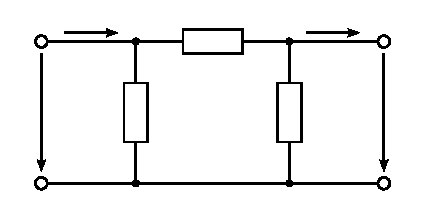
\includegraphics{Imatges/Cap-FluxCarregues-Trafo-Pi.pdf}
\caption{Circuit equivalent d'un transformaci\'{o} amb regulaci\'{o}
variable sense decalatge} \label{pic:equiv_trafo_reg}
\end{figure}

Els valors dels par\`{a}metres d'aquest circuit equivalent s\'{o}n:
\begin{align}
   \cmplx{Z}_\piup &= m \, \cmplx{Z}\ped{cc} \\[1.5ex]
   \cmplx{Y}_{\piup_1} &= \frac{1-m}{m^2 \,\cmplx{Z}\ped{cc}} \\[1.5ex]
   \cmplx{Y}_{\piup_2} &= \frac{m-1}{m\, \cmplx{Z}\ped{cc}}
\end{align}

\section{Tipus de nusos} \index{flux de c\`{a}rregues!tipus de nusos}

Cadascun dels nusos d'un sistema el\`{e}ctric de pot\`{e}ncia, t\'{e} quatre
magnituds associades: les potencies activa i reactiva injectades des
de l'exterior de la xarxa, i el m\`{o}dul i l'argument de la seva
tensi\'{o}.

Usualment, en cada nus del sistema es coneixen dues de les quatre
magnituds anteriors; segons quines siguin aquestes magnituds, es
poden distingir els seg\"{u}ents tipus de nusos:
\begin{dinglist}{'167}
    \item \textbf{Nus de potencial zero}. El terra \'{e}s sempre el nus de refer\`{e}ncia, o de potencial zero, de la
    xarxa, i per tant, totes les tensions de la xarxa hi s\'{o}n referides.
    Al terra s'assigna el n\'{u}mero de nus 0, i per tant no forma part de la matriu d'admit\`{a}ncies de nus de la xarxa.
\index{nus!de potencial zero}\index{nus!de refer\`{e}ncia}

   \item \textbf{Nus flotant}. \'{E}s un nus on es mant\'{e} constant la tensi\'{o} en m\`{o}dul i argument,
   essent inc\`{o}gnites les pot\`{e}ncies activa i reactiva injectades a la xarxa des de l'exterior.
    Generalment, acostuma a ser el nus que m\'{e}s s'aproxima a un nus de pot\`{e}ncia infinita. Des del
    punt de vista de la xarxa, correspon clarament a un generador ideal de tensi\'{o}.
    \index{nus!flotant}

Tan sols hi pot haver un nus d'aquest tipus en tota la xarxa.
   \item \textbf{Nus de tensi\'{o} controlada}. En aquest nus es coneix el m\`{o}dul de la tensi\'{o} i la
   pot\`{e}ncia activa injectada a la xarxa des de l'exterior, essent inc\`{o}gnites l'argument de la tensi\'{o} i la pot\`{e}ncia
   reactiva injectada des de l'exterior. En aquests nusos, sovint s'imposen l\'{\i}mits a la pot\`{e}ncia reactiva.
\index{nus!de tensi\'{o} controlada}

   \item \textbf{Nus de c\`{a}rrega}. En aquest nus es coneixen les pot\`{e}ncies activa i reactiva
   injectades a la xarxa des de l'exterior, i s\'{o}n inc\`{o}gnites el m\`{o}dul i l'argument de la tensi\'{o}.
   Aquests nusos poden ser tant de consum com de generaci\'{o}.
   \index{nus!de c\`{a}rrega}

En els nusos on incideix un transformador amb relaci\'{o} de
transformaci\'{o} variable sense decalatge, hi pot haver tres magnituds
conegudes: les pot\`{e}ncies activa i reactiva injectades i el m\`{o}dul de
la tensi\'{o}, el qual es vol mantenir constant mitjan\c{c}ant l'ajust de la
relaci\'{o} de transformaci\'{o}; les inc\`{o}gnites s\'{o}n per tant, l'argument de
la tensi\'{o} i la citada relaci\'{o} de transformaci\'{o} del transformador.
\end{dinglist}

En la Taula \vref{taula:tipus_nusos} es resumeix el que s'ha exposat
sobre els diferents tipus de nusos en un sistema el\`{e}ctric de
pot\`{e}ncia.
\begin{table}[htb]
   \caption{\label{taula:tipus_nusos} Tipus de nusos en un sistema el\`{e}ctric de pot\`{e}ncia}
   \begin{center}\begin{tabular}{lccccc}
   \toprule[1pt]
   \multirow{2}{15mm}{\rule{0mm}{4.5mm}Tipus\\de nus}  & \multicolumn{2}{c}{Tensi\'{o}} &
   \multicolumn{2}{c}{Pot\`{e}ncia injectada} & \renewcommand*{\multirowsetup}{\centering}
   \multirow{2}{25mm}{\rule{0mm}{4.5mm}Relaci\'{o} de\\transformaci\'{o}} \\
   \cmidrule(rl){2-3} \cmidrule(rl){4-5}
    & m\`{o}dul & argument & activa & reactiva &  \\
   \midrule
   Flotant                &  \textcolor{Green}{\ding{51}} & \textcolor{Green}{\ding{51}} & \textcolor{Red}{\ding{55}} & \textcolor{Red}{\ding{55}} & --- \\
   De tensi\'{o} controlada   &  \textcolor{Green}{\ding{51}} & \textcolor{Red}{\ding{55}} & \textcolor{Green}{\ding{51}} & \textcolor{Red}{\ding{55}} & --- \\
   De c\`{a}rrega (sense trafo)             &  \textcolor{Red}{\ding{55}} & \textcolor{Red}{\ding{55}} & \textcolor{Green}{\ding{51}} & \textcolor{Green}{\ding{51}} & --- \\
   De c\`{a}rrega (amb trafo) &  \textcolor{Green}{\ding{51}} & \textcolor{Red}{\ding{55}} & \textcolor{Green}{\ding{51}} & \textcolor{Green}{\ding{51}} & \textcolor{Red}{\ding{55}} \\

   \midrule
   \multicolumn{6}{c}{\textcolor{Green}{\ding{51}} valor conegut \hspace{6ex} \textcolor{Red}{\ding{55}} valor inc\`{o}gnita
   \hspace{6ex} --- no aplicable} \\
   \bottomrule[1pt]
   \end{tabular} \end{center}
\end{table}


\section{Formulaci\'{o} del problema}\label{sec:formul_prob} \index{flux de c\`{a}rregues!formulaci\'{o} del problema}

Comencem per considerar una xarxa el\`{e}ctrica amb els nusos numerats
$1,\ldots,n$, i essent el terra el nus 0 de refer\`{e}ncia; una de les
maneres de descriure aquesta xarxa \'{e}s utilitzant el m\`{e}tode dels
nusos, descrit en el Cap\'{\i}tol \ref{chap:nusos}:
\begin{equation}
    \mcmplx{Y}\ped{N} \mcmplx{V}\ped{N} = \mcmplx{J}\ped{N}
\end{equation}

Tenint en compte que els elements de $\mcmplx{J}\ped{N}$,
$\mcmplx{V}\ped{N}$ i $\mcmplx{Y}\ped{N}$ s\'{o}n $\cmplx{j}_i$,
$\cmplx{v}_i$ i  $\cmplx{y}_{ik}$ ($i,k=1,\ldots,n$) respectivament,
i que aquests valors, suposem que estan expressats en p.u. (vegeu la
Secci\'{o} \ref{sec:seccio_pu}), l'equaci\'{o} anterior queda expressada de
la seg\"{u}ent manera:
\begin{equation}
    \sum^n_{k=1}\, \cmplx{y}_{ik} \cmplx{v}_k = \cmplx{j}_i \qquad\qquad i=1,\ldots,n
\end{equation}

En cadascun dels nusos de la xarxa es compleix la seg\"{u}ent relaci\'{o}
per a la pot\`{e}ncia complexa $\cmplx{s}_i = p_i + \ju q_i$, injectada
al nus des de l'exterior:
\begin{equation}
    \cmplx{s}_i^* = p_i - \ju q_i = \cmplx{v}_i^* \cmplx{j}_i = \cmplx{v}_i^*
    \sum^n_{k=1}\, \cmplx{y}_{ik} \cmplx{v}_k \qquad\qquad i=1,\ldots,n \label{eq:sconj}
\end{equation}

Ara b\'{e}, si expressem els potencials $\cmplx{v}_i$ a partir dels seus m\`{o}duls $|\cmplx{v}_i|$
i arguments $\delta_i$, i les admit\`{a}ncies $\cmplx{y}_{ik}$ a partir de les seves parts
reals $g_{ik}$ i imagin\`{a}ries $b_{ik}$, tenim:
\begin{align}
    \cmplx{v}_i &=|\cmplx{v}_i| \eu^{\ju\delta_i} = |\cmplx{v}_i|
    (\cos\delta_i+\ju\sin\delta_i) & i & =1,\ldots,n\\
    \cmplx{y}_{ik} &= g_{ik} + \ju b_{ik} & i,k & =1,\ldots,n \\
    p_i - \ju q_i &= |\cmplx{v}_i| (\cos\delta_i - \ju\sin\delta_i) \sum^n_{k=1} (g_{ik} + \ju
    b_{ik}) |\cmplx{v}_k| (\cos\delta_k + \ju\sin\delta_k) & i & =1,\ldots,n
\end{align}

Finalment, si separem la darrera equaci\'{o} en dues, una per a  la part real i  una altra per
a la part imagin\`{a}ria, tenim:
\begin{align}
    p_i - |\cmplx{v}_i| \sum^n_{k=1}  |\cmplx{v}_k| \bigl[ g_{ik} \cos(\delta_k - \delta_i) -
     b_{ik} \sin(\delta_k - \delta_i) \bigr] &= 0  & i&=1,\ldots,n\label{eq:p0} \\
    q_i + |\cmplx{v}_i| \sum^n_{k=1}  |\cmplx{v}_k| \bigl[ g_{ik} \sin(\delta_k - \delta_i) +
      b_{ik} \cos(\delta_k - \delta_i) \bigr] &= 0 & i&=1,\ldots,n\label{eq:q0}
\end{align}

Resolent de forma simult\`{a}nia les equacions \eqref{eq:p0} i
\eqref{eq:q0}, trobar\'{\i}em els potencials dels nusos de la xarxa
respecte al terra, i posteriorment, utilitzant l'equaci\'{o}
\eqref{eq:sconj}, obtindr\'{\i}em la pot\`{e}ncia injectada en cada nus des
de l'exterior. Ara b\'{e}, \'{e}s clar que no es poden plantejar les
equacions \eqref{eq:p0} i \eqref{eq:q0} en tots els nusos de la
xarxa, ja que en alguns d'ells els valors $p_i$ o $q_i$ s\'{o}n
desconeguts (vegeu la Taula \vref{taula:tipus_nusos}). Per tant, per
tal de resoldre el problema del flux de c\`{a}rregues en un sistema
el\`{e}ctric de pot\`{e}ncia, cal seguir els passos seg\"{u}ents:
\begin{dingautolist}{'312}
    \item Es numeren tots els nusos de la xarxa, comen\c{c}ant pel n\'{u}mero 1. El terra \'{e}s sempre el nus 0 de refer\`{e}ncia.
   \item Es forma la matriu d'admit\`{a}ncies de nusos $\mcmplx{Y}\ped{N}$, tal com s'ha
   explicat en el Cap\'{\i}tol \ref{chap:nusos}.
   \item Es forma l'equaci\'{o} \eqref{eq:p0} per a tots els nusos de tensi\'{o} controlada i per
   a tots els nusos de c\`{a}rrega. Cal tenir en compte que la pot\`{e}ncia activa  injectada $p_i$ es considera
   positiva quan entra des de l'exterior a la xarxa, i negativa en cas contrari.
   \item Es forma l'equaci\'{o} \eqref{eq:q0} per a tots els nusos de c\`{a}rrega. Cal tenir en compte
   que la pot\`{e}ncia reactiva injectada $q_i$  es considera positiva quan entra des de l'exterior a la xarxa, i negativa en cas contrari.
   \item Es resol de forma num\`{e}rica el sistema d'equacions no lineals, format en els dos
   passos anteriors; com a valors inicials de les inc\`{o}gnites, es poden prendre els valors
   seg\"{u}ents:
   \begin{dinglist}{'167}
    \item M\`{o}duls dels potencials: m\`{o}dul del potencial del nus flotant
    \item Arguments dels potencials: argument del potencial del nus flotant
    \item Relacions de transformaci\'{o}: 1
   \end{dinglist}
   \item Si \'{e}s necessari,  es pot calcular la pot\`{e}ncia injectada en els nusos de la xarxa
   des de l'exterior, en aquells nusos on no es
   coneix aquest valor, utilitzant    l'equaci\'{o} \eqref{eq:sconj}.
\end{dingautolist}

\begin{exemple}
Es tracta de trobar en la xarxa seg\"{u}ent, els potencials dels nusos 2
i 3, i les pot\`{e}ncies subministrades pels generador dels nusos 1 i 2;
tots els valors estan donats en p.u.
\begin{figure}[htb]
\centering
    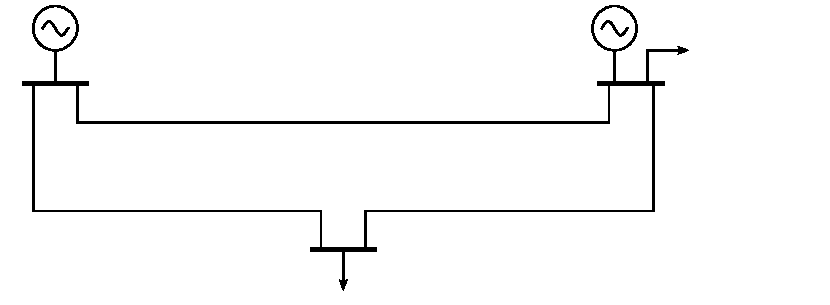
\includegraphics{Imatges/Cap-FluxCarregues-Exemple1.pdf}
\end{figure}

Comencem formant la matriu d'admit\`{a}ncies de nus:
\begin{align*}
\mcmplx{Y}\ped{N} &= \begin{pmatrix}
\frac{1}{0{,}028+\ju0{,}096} + \frac{1}{0{,}01+\ju0{,}03} & -\frac{1}{0{,}028+\ju0{,}096}  &  -\frac{1}{0{,}01+\ju0{,}03}\\
-\frac{1}{0{,}028+\ju0{,}096} & \frac{1}{0{,}028+\ju0{,}096} + \frac{1}{0{,}02+\ju0{,}06} &  -\frac{1}{0{,}02+\ju0{,}06}\\
-\frac{1}{0{,}01+\ju0{,}03} & -\frac{1}{0{,}02+\ju0{,}06} &
\frac{1}{0{,}01+\ju0{,}03} + \frac{1}{0{,}02+\ju0{,}06}
\end{pmatrix} = \\[1.5ex]
 &= \begin{pmatrix}
12{,}8 - \ju 39{,}6 & -2{,}8 + \ju 9{,}6 & -10{,}0 + \ju 30{,}0 \\
-2{,}8 + \ju 9{,}6 & 7{,}8 - \ju 24{,}6 & -5{,}0 + \ju 15{,}0 \\
-10{,}0 + \ju 30{,}0 & -5{,}0 + \ju 15{,}0 & 15{,}0 - \ju 45{,}0
\end{pmatrix}
\end{align*}

El nus 1 \'{e}s el nus flotant, el nus 2 en un nus de tensi\'{o} controlada
i el nus 3 \'{e}s un nus de c\`{a}rrega; formarem, per tant, l'equaci\'{o}
\eqref{eq:p0} pels nusos 2 i 3, i l'equaci\'{o} \eqref{eq:q0} pel nus 3:
\begin{align*}
\begin{split}
0{,}25-0{,}5 &- 1{,}03\cdot \bigl( 1{,}05\cdot [-2{,}8
\cdot\cos(-\delta_2) - 9{,}6
\cdot\sin( -\delta_2)]  + 1{,}03 \cdot 7{,}8 {}+ \\
&+ |\cmplx{v}_3|\cdot [-5{,}0 \cdot\cos(\delta_3-\delta_2) -
15{,}0\cdot \sin(\delta_3-\delta_2)]
 \bigr)  = 0 \end{split} \\[1.5ex]
\begin{split}
-0{,}6 &- |\cmplx{v}_3| \cdot \bigl( 1{,}05\cdot [-10{,}0
\cdot\cos(-\delta_3)
- 30{,}0\cdot\sin(-\delta_3)]  + \\
&+ 1{,}03\cdot [-5{,}0\cdot\cos(\delta_2-\delta_3) -
15{,}0\cdot\sin(\delta_2-\delta_3)]
 + |\cmplx{v}_3| \cdot15{,}0 \bigr)  = 0 \end{split}  \\[1.5ex]
\begin{split}
-0{,}3 &+ |\cmplx{v}_3|\cdot \bigl( 1{,}05
\cdot[-10{,}0\cdot\sin(-\delta_3) +
30{,}0\cdot\cos(-\delta_3)]  + \\
&+ 1{,}03 \cdot[-5{,}0\cdot\sin(\delta_2-\delta_3) +
15{,}0\cdot\cos(\delta_2-\delta_3)] + |\cmplx{v}_3|\cdot (-45{,}0)
\bigr)  = 0 \end{split}
\end{align*}

Resolent aquest sistema d'equacions no lineals, amb els valors
inicials $|\cmplx{v}_3|=1{,}05$ i $\delta_2=\delta_3=0$, obtenim:
\begin{gather*}
   \delta_2=-0{,}015277\unit{rad} \\[1ex]
   |\cmplx{v}_3|=1{,}033587 \qquad \delta_3=-0{,}014301\unit{rad}
\end{gather*}

Calcularem a continuaci\'{o}, les pot\`{e}ncies injectades en els nusos 1 i
2, utilitzant l'equaci\'{o} \eqref{eq:sconj}:
\begin{align*}
\begin{split}
\cmplx{s}_1^* &= 1{,}05 \cdot\bigl[ (12{,}8-\ju39{,}6) \cdot 1{,}05
+
(-2{,}8+\ju9{,}6) \cdot 1{,}03\cdot\eu^{-\ju0{,}015277} + \\
&+ (-10{,}0+\ju30{,}0) \cdot 1{,}033587\cdot\eu^{-\ju0{,}014301}
\bigr] = 0{,}85680 - \ju 0{,}52169
\end{split} \\[1.5ex]
\cmplx{s}_1 &= 0{,}85680 + \ju 0{,}52169 \\[1.5ex]
\begin{split}
\cmplx{s}_2^* &= 1{,}03 \cdot\eu^{\ju0{,}015277} \cdot\bigl[
(-2{,}8+\ju9{,}6) \cdot 1{,}05 +
 (7{,}8-\ju24{,}6) \cdot 1{,}03\cdot\eu^{-\ju0{,}015277} + \\
& + (-5{,}0+\ju15{,}0) \cdot 1{,}033587\cdot\eu^{-\ju0{,}014301}
\bigr] = -0{,}25000 + \ju 0{,}20050
\end{split} \\[1.5ex]
 \cmplx{s}_2 &= -0{,}25000 - \ju 0{,}20050
\end{align*}

Per tant, les pot\`{e}ncies subministrades a la xarxa pels generadors
dels nusos 1 i 2, s\'{o}n:
\begin{align*}
\cmplx{s}\ped{G1} &= \cmplx{s}_1 = 0{,}85680 + \ju 0{,}52169 \\[1ex]
\cmplx{s}\ped{G2} &= \cmplx{s}\ped{L2} + \cmplx{s}_2 = 0{,}5 + \ju
0{,}25 -0{,}25000 - \ju 0{,}20050  = 0{,}25000 + \ju 0{,}04950
\end{align*}

El valor calculat de la pot\`{e}ncia activa subministrada pel generador
del nus 2, es
 correspon, evidentment, amb el valor que s'ha utilitzat com a dada per
resoldre la xarxa ($p\ped{G2}=0{,}25$).

Pel que fa a la potencia reactiva subministrada pel generador del
nus 2, s'observa que es troba dins dels  marges especificats
($-0{,}1<q\ped{G2}<0{,}2$).
\end{exemple}

\begin{exemple}

Es tracta de trobar en la xarxa seg\"{u}ent, el potencial del nus 2 i la
pot\`{e}ncia subministrada pel generador del nus 1; tots els valors
estan donats en p.u. Es consideren dos casos:
\begin{enumerate}
   \renewcommand{\labelenumi}{\alph{enumi})}
   \item La bateria de condensadors del nus 2 est\`{a} desconnectada.
   \item Es connecta la bateria de condensadors del nus 2, per tal de mantenir el m\`{o}dul de
   la tensi\'{o} d'aquest nus al valor $|\cmplx{v}_2|=1{,}03$.
\end{enumerate}
\begin{figure}[htb]
\centering
    
\includegraphics{Imatges/Cap-FluxCarregues-Exemple2.pdf}
\end{figure}

Comencem formant la matriu d'admit\`{a}ncies de nus:
\[
\mcmplx{Y}\ped{N} = \begin{pmatrix}
  \frac{\ju 0{,}10}{2} + \frac{1}{0{,}028+\ju0{,}096} & -\frac{1}{0{,}028+\ju0{,}096} \\
  -\frac{1}{0{,}028+\ju0{,}096} & \frac{\ju 0{,}10}{2} + \frac{1}{0{,}028+\ju0{,}096} \\
\end{pmatrix} =
\begin{pmatrix}
  2{,}80 -\ju9{,}55 & -2{,}80 +\ju9{,}60 \\
  -2{,}80 +\ju9{,}60 & 2{,}80 -\ju9{,}55 \\
\end{pmatrix}
\]

a) En aquest cas, el nus 1 \'{e}s el nus flotant, i el nus 2 en un nus
de c\`{a}rrega.

Formem a continuaci\'{o} les equacions \eqref{eq:p0} i \eqref{eq:q0} pel
nus 2:
\begin{align*}
-0{,}8 - |\cmplx{v}_2| \cdot \bigl( 1{,}05\cdot [-2{,}80\cdot \cos(-\delta_2) - 9{,}60 \cdot
\sin( -\delta_2)]  + |\cmplx{v}_2| \cdot 2{,}80 \bigr) &= 0 \\
-0{,}6 + |\cmplx{v}_2| \cdot\bigl( 1{,}05 \cdot[-2{,}80\cdot\sin(-\delta_2) +
9{,}60\cdot\cos( -\delta_2)]  + |\cmplx{v}_2|\cdot (-9{,}55) \bigr) &= 0
\end{align*}

Resolent aquest sistema d'equacions no lineals, amb els valors inicials $|\cmplx{v}_2|=1{,}05$ i $\delta_2=0$, obtenim:
\[ |\cmplx{v}_2|=0{,}970306 \qquad \delta_2=-0{,}060222\unit{rad} \]

Calculem a continuaci\'{o} la pot\`{e}ncia que circula des del nus 1 cap al
nus 2, utilitzant l'equaci\'{o} \eqref{eq:lin_s12}:
\[
\cmplx{s}_{12} = 1{,}05\cdot \left[ \frac{\ju0{,}10}{2} \cdot1{,}05 + \frac{ 1{,}05 -
0{,}970306\cdot\eu^{-\ju0{,}060222}} {0{,}028+\ju0{,}096} \right]^* = 0{,}82813 + \ju
0{,}59423
\]

Per tant, la pot\`{e}ncia subministrada a la xarxa pel generador del nus
1, \'{e}s:
\[ \cmplx{s}\ped{G1} = \cmplx{s}\ped{L1} + \cmplx{s}_{12} = 1{,}2+\ju0{,}3 + 0{,}82812 + \ju 0{,}59423 = 2{,}02813 + \ju 0{,}89423 \]

b) En aquest cas, el nus 1 \'{e}s el nus flotant, i el nus 2 en un nus
de tensi\'{o} controlada.

Formem a continuaci\'{o} l'equaci\'{o} \eqref{eq:p0} pel nus 2:
\[
-0{,}8 - 1{,}03\cdot \bigl( 1{,}05\cdot [-2{,}80\cdot\cos(-\delta_2) - 9{,}60\cdot\sin(
-\delta_2)] + 1{,}03\cdot 2{,}80 \bigr) = 0
\]

Resolent aquesta equaci\'{o} no lineal, amb el valor inicial $\delta_2=0$, obtenim:
\[\delta_2=-0{,}072323\unit{rad}\]

Calculem a continuaci\'{o} la pot\`{e}ncia que circula entre els nusos 1 i
2, utilitzant les equacions \eqref{eq:lin_s12} i \eqref{eq:lin_s21}:
\begin{align*}
\cmplx{s}_{12} &= 1{,}05 \cdot\left[ \frac{\ju0{,}10}{2} \cdot1{,}05 + \frac{ 1{,}05 -
1{,}03\cdot\eu^{-\ju0{,}072323}} {0{,}028+\ju0{,}096} \right]^* =
0{,}81695 - \ju 0{,}04520 \\[1.5ex]
\cmplx{s}_{21} &= 1{,}03\cdot \eu^{-\ju0{,}072323} \cdot\left[ \frac{\ju0{,}10}{2}\cdot
1{,}03\cdot \eu^{-\ju0{,}072323} + \frac{ 1{,}03\cdot\eu^{-\ju0{,}072323} -1{,}05}
{0{,}028+\ju0{,}096} \right]^* = -0{,}80000 - \ju 0{,}00484
\end{align*}

Per tant, les pot\`{e}ncies subministrades a la xarxa pel generador del
nus 1 i pel condensador del nus 2, s\'{o}n:
\begin{align*}
 \cmplx{s}\ped{G1} &= \cmplx{s}\ped{L1} + \cmplx{s}_{12} = 1{,}2+\ju0{,}3 + 0{,}81695 - \ju 0{,}04520 = 2{,}01695 + \ju 0{,}25480 \\
 \cmplx{s}\ped{Q2} &= \cmplx{s}\ped{L2} + \cmplx{s}_{21} = 0{,}8+\ju0{,}6 - 0{,}80000 - \ju 0{,}00484 =  \ju 0{,}59516
\end{align*}

S'ha calculat el valor de $\cmplx{s}\ped{Q2}$, per tal de comprovar
que est\`{a} dins dels marges especificats
($|\cmplx{s}\ped{Q2}|_{\text{m\`{a}x.}}=0{,}6$); si aix\`{o} no fos aix\'{\i},
caldria fixar $\cmplx{s}\ped{Q2}$ al seu valor m\`{a}xim i tornar a
recalcular la xarxa, passant el nus 2 a ser un nus de c\`{a}rrega, i
essent, per tant, desconeguda la seva tensi\'{o}.
\end{exemple}

\break
\begin{exemple}
En el sistema de la figura seg\"{u}ent, es vol mantenir el m\`{o}dul del
potencial del nus 2 fixat al valor indicat, mitjan\c{c}ant l'ajust
adequat de la relaci\'{o} de transformaci\'{o} del transformador connectat
entre els nusos 1 i 2. Es tracta per tant de trobar aquest valor,
aix\'{\i} com el potencial del nus 2; tots els valors estan donats en
p.u.

\begin{figure}[h!]
\centering
    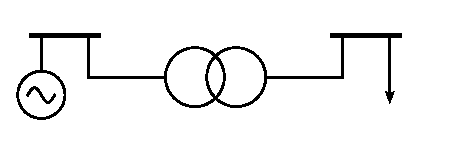
\includegraphics{Imatges/Cap-FluxCarregues-Exemple3.pdf}
\end{figure}

Comencem formant la matriu d'admit\`{a}ncies de nus:
\[
\mcmplx{Y}\ped{N} = \begin{pmatrix}
\dfrac{1}{\ju0{,}02 \,m^2}  &  -\dfrac{1}{\ju0{,}02 \,m} \\[1.5ex]
-\dfrac{1}{\ju0{,}02\, m}   & \dfrac{1}{\ju0{,}02}
\end{pmatrix} =
\begin{pmatrix}
-\ju\dfrac{50}{m^2}  &  \ju\dfrac{50}{m} \\[1.5ex]
\ju\dfrac{50}{m}     & -\ju 50
\end{pmatrix}
\]

El nus 1 \'{e}s el nus flotant i el nus 2 en un nus de c\`{a}rrega;
formarem, per tant,  les equacions \eqref{eq:p0} i \eqref{eq:q0} pel
nus 2:
\begin{align*}
-2 - 1 \cdot\left( 1 \cdot\left[ 0 -\frac{50}{m} \cdot\sin(-\delta_2) \right]  + 0 \right)  = 0   \\[1.5ex]
-1 + 1 \cdot\left( 1 \cdot\left[0 + \frac{50}{m}
\cdot\cos(-\delta_2) \right]  + 1\cdot (-50) \right)  = 0
\end{align*}

Resolent aquest sistema d'equacions no lineals, amb els valors
inicials $\delta_2=0$ i $m=1$, obtenim:
\begin{align*}
   \delta_2 &= -0{,}039196\unit{rad} \\[1ex]
   m & =0{,}979639
\end{align*}

En un cas real, el par\`{a}metre $m$ del transformador \'{u}nicament podria
prendre uns quants valors discrets; caldria doncs assignar a $m$ el
valor m\'{e}s pr\`{o}xim al calculat, escollint entre els diversos valors
possibles, i tornar a recalcular la xarxa, passant la tensi\'{o} del nus
2 a ser un valor desconegut.

\end{exemple}

\section{Control del flux de pot\`{e}ncia} \index{flux de c\`{a}rregues!control del flux de
pot\`{e}ncia}\label{sec:control-flux-pot}

Veurem breument a continuaci\'{o}, les diverses formes que existeixen
per controlar el flux de pot\`{e}ncia activa i reactiva en les branques
d'una xarxa, aix\'{\i} com els m\`{e}todes que existeixen per mantenir la
tensi\'{o} regulada en determinats nusos.

En concret, es disposa dels seg\"{u}ents m\`{e}todes:

\begin{dinglist}{'167}
   \item \textbf{Control de l'excitaci\'{o} i del parell motriu dels generador}. \'{E}s prou conegut,
    que variant l'excitaci\'{o} d'un generador, podem regular la seva tensi\'{o} de sortida o
        la pot\`{e}ncia reactiva que subministra al sistema; d'altra banda, variant el parell motriu,
    podem regular la freq\"{u}\`{e}ncia de la tensi\'{o} de sortida o la pot\`{e}ncia activa que subministra al sistema.

    En el cas d'un generador a\"{\i}llat que alimenta a una c\`{a}rrega
    donada, la qual fixa la pot\`{e}ncia activa i reactiva necess\`{a}ries, variant
     l'excitaci\'{o} o el parell motriu del
    generador podem regular respectivament, el valor de la tensi\'{o}
    o de la freq\"{u}\`{e}ncia de sortida. En el cas d'un generador acoblat a una xarxa de pot\`{e}ncia
    infinita, la qual fixa els valors de la tensi\'{o} i de la freq\"{u}\`{e}ncia, variant l'excitaci\'{o} o el parell motriu del
    generador podem regular respectivament, el valor de la pot\`{e}ncia reactiva o de la pot\`{e}ncia
    activa  subministra al sistema.

   \item \textbf{Variaci\'{o} de les caracter\'{\i}stiques de condensadors i react\`{a}ncies, s\`{e}rie
    i para{\l.l}el}. Aquest m\`{e}tode s'utilitza per mantenir regulada la tensi\'{o} en determinats
     nusos del sistema, dins d'uns certs marges prefixats, mitjan\c{c}ant la injecci\'{o}  de pot\`{e}ncia
      reactiva, aportada per condensadors i react\`{a}ncies.

   \item \textbf{Ajust adequat dels transformadors de relaci\'{o} de transformaci\'{o} variable amb
    decalatge}. La funci\'{o} usual dels transformadors en els sistemes el\`{e}ctrics de pot\`{e}ncia,
    \'{e}s passar la tensi\'{o} d'un nivell determinat a un altre, per exemple, de la tensi\'{o} de generaci\'{o}
    a la tensi\'{o} de la l\'{\i}nia de transmissi\'{o}. No obstant, en els sistemes de pot\`{e}ncia, tamb\'{e} existeixen
    transformadors dedicats al control del flux de pot\`{e}ncia activa i reactiva en determinades
    branques; aix\`{o} s'aconsegueix amb petites variacions de la relaci\'{o} de transformaci\'{o} i del
    decalatge del transformador. La variaci\'{o} del decalatge, t\'{e} un gran efecte sobre el flux
    de pot\`{e}ncia activa, a l'hora que pr\`{a}cticament no afecta al flux de pot\`{e}ncia reactiva ni al
    m\`{o}dul de la tensi\'{o}; en canvi, la variaci\'{o} de la relaci\'{o} de transformaci\'{o} t\'{e} un gran efecte
    sobre el flux de pot\`{e}ncia reactiva i sobre al m\`{o}dul de la tensi\'{o}.
\end{dinglist}

\section{\texorpdfstring{Resoluci\'{o} de sistemes d'equacions no lineals amb \textit{Mathematica}${}^\circledR$ i \textit{MATLAB}${}^\circledR$}{Resoluci\'{o} de sistemes d'equacions no lineals amb Mathematica� i MATLAB�}}
\label{sec:sis_eq_no_lin}
\index{Mathematica@\textit{Mathematica}${}^\circledR$}
\index{MATLAB@\textit{MATLAB}${}^\circledR$}

En aquest apartat, es descriu breument com trobar la soluci\'{o} d'un sistema d'equacions no lineals, com els que sorgeixen a l'hora de resoldre problemes de flux de c\`{a}rregues, amb els programes \textit{Mathematica}${}^\circledR$ i \textit{MATLAB}${}^\circledR$.

S'utilitzar\`{a} en ambd\'{o}s casos els sistema d'equacions no lineals del segon exemple de la secci\'{o} \ref{sec:formul_prob}, \'{e}s a dir:
\begin{align*}
-0{,}8 - |\cmplx{v}_2| \cdot \bigl( 1{,}05\cdot [-2{,}80\cdot \cos(-\delta_2) - 9{,}60 \cdot
\sin( -\delta_2)]  + |\cmplx{v}_2| \cdot 2{,}80 \bigr) &= 0 \\
-0{,}6 + |\cmplx{v}_2| \cdot\bigl( 1{,}05 \cdot[-2{,}80\cdot\sin(-\delta_2) +
9{,}60\cdot\cos( -\delta_2)]  + |\cmplx{v}_2|\cdot (-9{,}55) \bigr) &= 0
\end{align*}

Els valors inicials assignats a les dues variables s\'{o}n: $|\cmplx{v}_2|=1{,}05$ i $\delta_2=0$.

La resoluci\'{o} d'aquest sistema d'equacions no lineals amb el programa \textit{Mathematica}${}^\circledR$ \'{e}s molt senzilla, ja que la funci\'{o} \texttt{FindRoot} ens proporciona directament la soluci\'{o}; utilitzant la variable \texttt{v2} per a $|\cmplx{v}_2|$ i la variable \texttt{d2} per a $\delta_2$, tenim:

\begin{alltt}
\bfseries\small In[1]:= FindRoot[\{-0.8 - v2 (1.05 (-2.8 Cos[-d2] - 9.6 Sin[-d2]) + 2.8 v2) == 0,
                 -0.6 + v2 (1.05 (-2.8 Sin[-d2] + 9.6 Cos[-d2]) - 9.55 v2) == 0\},
                 \{v2, 1.05\}, \{d2, 0.0\}]\\
Out[1]:= \{v2 -> 0.970306, d2 -> -0.0602217\}
\end{alltt}

La resoluci\'{o} amb el programa \textit{MATLAB}${}^\circledR$ no \'{e}s tan senzilla, i s'obt\'{e} a partir de la funci\'{o}  \texttt{fsolve}; per poder utilitzar aquesta funci\'{o}, cal tenir insta{\l.l}ada l'extensi\'{o} del programa {"<}Optimization toolbox{">}.

En primer lloc, cal escriure una funci\'{o} en un {"<}fitxer M{">} que representi el sistema d'equacions no lineals que es vol resoldre; utilitzant la variable \texttt{x(1)} per a $|\cmplx{v}_2|$ i la variable \texttt{x(2)} per a $\delta_2$, creem un fitxer amb el contingut seg\"{u}ent:

\begin{alltt}
\bfseries\small{}function y= F(x)
y(1) = -0.8 - x(1)*(1.05*(-2.8*cos(-x(2)) - 9.6*sin(-x(2))) + 2.8*x(1));
y(2) = -0.6 + x(1)*(1.05*(-2.8*sin(-x(2)) + 9.6*cos(-x(2))) - 9.55*x(1));
\end{alltt}

A continuaci\'{o} resolem el sistema d'equacions no lineal, utilitzant la funci\'{o} \texttt{fsolve}:

\begin{alltt}
\bfseries\small>> fsolve(@F, [1.05; 0.0])\\
ans =\\
    0.9703
   -0.0602
\end{alltt}




      \appendix
   \part{Ap\`{e}ndixs}
      \renewcommand*{\chaptername}{\appendixname}
      \chapter{Escales Logar\'{\i}tmiques} \index{escales logar\'{\i}tmiques}

En diferents camps de l'electrot\`{e}cnia, \'{e}s usual trobar-se gr\`{a}fics amb escales
logar\'{\i}tmiques.

Un exemple clar, s\'{o}n els gr\`{a}fics d'actuaci\'{o} dels interruptors magnetot\`{e}rmics o dels
fusibles, on les seves corbes caracter\'{\i}stiques intensitat--temps estan representades en
una escala logar\'{\i}tmica--logar\'{\i}tmica o lineal--logar\'{\i}tmica.

En aquests casos, es presenta freq\"{u}entment la necessitat de determinar amb exactitud un
punt de la corba, que no coincideix amb cap de les l\'{\i}nies divis\`{o}ries del gr\`{a}fic. Atenent a
la Figura \vref{pic:escala log}, es tractaria de determinar el valor $x$ dins de la d\`{e}cada
$10^N$ a $10^{N+1}$.

\begin{figure}[htb]
\vspace{5mm} \centering \PSforPDF{
    %Created by jPicEdt 1.x
    %PsTricks format (pstricks.sty needed)
    %Sat Sep 11 16:54:36 CEST 2004
    \psset{xunit=1mm,yunit=1mm,runit=1mm}
    \begin{pspicture}(0,0)(150.00,40.00)
    \psline[linewidth=0.25,linecolor=black]{-}(0.00,29.00)(150.00,29.00)
    \psline[linewidth=0.25,linecolor=black]{-}(5.00,34.00)(5.00,24.00)
    \psline[linewidth=0.25,linecolor=black]{-}(47.00,34.00)(47.00,24.00)
    \psline[linewidth=0.25,linecolor=black]{-}(72.00,34.00)(72.00,24.00)
    \psline[linewidth=0.25,linecolor=black]{-}(89.00,34.00)(89.00,24.00)
    \psline[linewidth=0.25,linecolor=black]{-}(103.00,34.00)(103.00,24.00)
    \psline[linewidth=0.25,linecolor=black]{-}(113.00,34.00)(113.00,24.00)
    \psline[linewidth=0.25,linecolor=black]{-}(123.00,34.00)(123.00,24.00)
    \psline[linewidth=0.25,linecolor=black]{-}(131.00,34.00)(131.00,24.00)
    \psline[linewidth=0.25,linecolor=black]{-}(138.00,34.00)(138.00,24.00)
    \psline[linewidth=0.25,linecolor=black]{-}(145.00,34.00)(145.00,24.00)
    \pscircle[linewidth=0.25,linecolor=black,fillcolor=black,fillstyle=solid](33.00,29.00){1.00}
    \rput[b](33.00,36.00){$x$} \rput[b](145.00,36.00){$10^{N+1}$}
    \rput[b](5.00,36.00){$10^N$}
    \psline[linewidth=0.25,linecolor=black,linestyle=dashed,dash=1.00
    1.00]{-}(5.00,22.85)(5.00,0.00)
    \psline[linewidth=0.25,linecolor=black,linestyle=dashed,dash=1.00
    1.00]{-}(33.00,27.00)(33.00,11.42)
    \psline[linewidth=0.25,linecolor=black,linestyle=dashed,dash=1.00
    1.00]{-}(145.00,22.85)(145.00,0.00)
    \psline[linewidth=0.25,linecolor=black]{<->}(5.00,2.50)(145.00,2.50)
    \rput[b](19.00,15.00){$D$} \rput[b](77.00,4.00){$L$}
    \psline[linewidth=0.25,linecolor=black]{<->}(5.00,13.00)(33.00,13.00)
    \psline[linewidth=0.25,linecolor=black]{->}(33.00,34.00)(33.00,31.00)
\end{pspicture}
}
\caption{Escala logar\'{\i}tmica} \label{pic:escala log}
\end{figure}

Si mesurem amb un regle la dist\`{a}ncia $D$ des de l'inici de la d\`{e}cada fins al punt $x$, i
la longitud total $L$ de la d\`{e}cada, el valor $x$ buscat ve donat per l'expressi\'{o}:
\begin{equation}
    x = 10^{\left(N+\frac{D}{L}\right)}
\end{equation}

Si estem interessats en el problema invers, \'{e}s a dir, en  trobar la dist\`{a}ncia $D$
corresponent a un valor conegut $x$ dins de la d\`{e}cada $10^N$ a $10^{N+1}$, podem emprar
l'expressi\'{o}:
\begin{equation}
    D = L(\log x - N) = L \log\frac{x}{10^N}
\end{equation}

\begin{exemple}
Es tracta de trobar el valor $x$ dins de la d\`{e}cada 100 a 1000, corresponent a una
dist\`{a}ncia $D=11\unit{mm}$; la longitud total de la d\`{e}cada \'{e}s $L=56\unit{mm}$.

En aquest cas tenim $N=2$, i per tant:
\[
    x = 10^{\left(2+\frac{11\unit{mm}}{56\unit{mm}}\right)}= 157{,}19
\]
\end{exemple}

\begin{exemple}
Es tracta de trobar la dist\`{a}ncia $D$ a la qual hem de dibuixar el valor $x=5$, dins de la
d\`{e}cada 1 a 10; la longitud total de la d\`{e}cada \'{e}s $L=56\unit{mm}$.

En aquest cas tenim $N=0$, i per tant:
\[
    D = 56\unit{mm} \cdot (\log 5 - 0)  = 39{,}1\unit{mm}
\]
\end{exemple}

      \include{Ape-Resistencies}
      \chapter{Grau de Protecci\'{o} IP} \index{IP} \index{grau de protecci\'{o}} \index{CEI!60529}

La codificaci\'{o} {"<}International Protection{">} (\textsf{IP}), segons la
norma \textsf{CEI 60529}, s'utilitza per descriure el grau de
protecci\'{o}  proporcionat per les envolvents d'equips el\`{e}ctrics, contra
la penetraci\'{o} de cossos s\`{o}lids estranys i contra els efectes nocius
de l'aigua.

\section{Codificaci\'{o}}
 La codificaci\'{o} consisteix en les sigles \textsf{\textbf{IP}}
seguides per dues xifres, m\'{e}s una lletra addicional (opcional) i una
lletra suplement\`{a}ria (opcional); quan el grau de protecci\'{o}
corresponent a una de les dues xifres no s'utilitzi, perqu\`{e} no sigui
necessari o perqu\`{e} no sigui conegut, es reempla\c{c}ar\`{a} la xifra en
q\"{u}esti\'{o} per una \textsf{\textbf{X}}. Es defineix a continuaci\'{o} el
significat de les xifres i lletres que formen el codi \textsf{IP}:

\textbf{1a xifra}. Indica el grau de protecci\'{o} de les persones contra els contactes amb
parts en tensi\'{o}, o amb peces en moviment, i el grau de protecci\'{o} dels equips contra la
penetraci\'{o} de cossos s\`{o}lids i pols. Els valors possibles s\'{o}n els seg\"{u}ents:
\begin{multicols}{2}
\begin{list}{}
   {\setlength{\labelwidth}{4.5mm} \setlength{\leftmargin}{4.5mm} \setlength{\labelsep}{2mm}}
   \item[\textbf{0}] Sense protecci\'{o}.
   \item[\textbf{1}] Protegit contra l'entrada de cossos s\`{o}lids superiors a 50\unit{mm},
   com per exemple,   contactes involuntaris de la m\`{a}.
   \item[\textbf{2}] Protegit contra l'entrada de cossos superiors a 12,5\unit{mm}, com per exemple,
   contactes involuntaris dels dits de la m\`{a}.
   \item[\textbf{3}] Protegit contra l'entrada de cossos superiors a 2,5\unit{mm},
   com per exemple, eines o cables.
   \item[\textbf{4}] Protegit contra l'entrada de cossos superiors a 1\unit{mm}.
   \item[\textbf{5}] Protegit contra la pols. Es permet la seva entrada all\`{a} on no sigui perjudicial.
   \item[\textbf{6}] Protegit totalment contra la pols.
\end{list}
\end{multicols}

\textbf{2a xifra}. Indica el grau de protecci\'{o} dels equips contra
l'entrada d'aigua. Els valors possibles s\'{o}n els seg\"{u}ents: \pagebreak
\begin{multicols}{2}
\begin{list}{}
   {\setlength{\labelwidth}{4.5mm} \setlength{\leftmargin}{4.5mm} \setlength{\labelsep}{2mm}}
   \item[\textbf{0}] Sense protecci\'{o}.
   \item[\textbf{1}] Protegit contra la caiguda vertical d'aigua.
   \item[\textbf{2}] Protegit contra la caiguda d'aigua, fins a 15\unit{\degree} de la  vertical.
   \item[\textbf{3}] Protegit contra la caiguda d'aigua, fins a 60\unit{\degree} de la  vertical.
   \item[\textbf{4}] Protegit contra la caiguda d'aigua, en totes les direccions.
   \item[\textbf{5}] Protegit contra aigua llan\c{c}ada per m\`{a}negues.
   \item[\textbf{6}] Protegit contra aigua llan\c{c}ada per cops de mar.
   \item[\textbf{7}] Protegit contra la immersi\'{o} temporal.
   \item[\textbf{8}] Protegit contra la immersi\'{o} prolongada, o a gran pressi\'{o}.
\end{list}
\end{multicols}

\textbf{Lletra addicional (opcional)}. En alguns casos la protecci\'{o}
proporcionada per les envolvents contra l'acc\'{e}s a les parts
perilloses \'{e}s millor que la indicada per la primera xifra del codi;
en aquests casos, es pot caracteritzar aquesta protecci\'{o} amb una
lletra addicional, afegida despr\'{e}s de les dues xifres; aix\`{o} permet
tenir obertures adequades per a la ventilaci\'{o},  guardant a l'hora el
grau requerit de protecci\'{o} de les persones. Els valors possibles s\'{o}n
els seg\"{u}ents:
\begin{multicols}{2}
\begin{list}{}
   {\setlength{\labelwidth}{5mm} \setlength{\leftmargin}{5mm} \setlength{\labelsep}{2mm}}
   \item[\textbf{A}] Els  cossos estranys de di\`{a}metre superior a
   50\unit{mm},
    poden penetrar en l'envolvent, per\`{o} tan sols d'una forma volunt\`{a}ria i deliberada.
   \item[\textbf{B}] Els  cossos estranys de di\`{a}metre superior a 12,5\unit{mm}
    poden penetrar en l'envolvent, per\`{o} un dit de la m\`{a} no ha de poder entrar m\'{e}s de 80\unit{mm}, i
    ha de quedar per tant, a una dist\`{a}ncia    suficient de les parts perilloses.
   \item[\textbf{C}] Els  cossos estranys de di\`{a}metre superior a 2,5\unit{mm}
   poden penetrar en l'envolvent, per\`{o} un filferro d'acer d'aquest di\`{a}metre i 100\unit{mm}
   de longitud, ha de quedar a una dist\`{a}ncia suficient de les parts perilloses.
   \item[\textbf{D}] Els  cossos estranys de di\`{a}metre superior a 1\unit{mm}
   poden penetrar en l'envolvent, per\`{o} un filferro d'acer d'aquest di\`{a}metre i 100\unit{mm}
   de longitud, ha de quedar a una dist\`{a}ncia suficient de les parts perilloses.
\end{list}
\end{multicols}

\textbf{Lletra suplement\`{a}ria (opcional)}. El codi \textsf{IP} accepta tamb\'{e} algunes
lletres suplement\`{a}ries al final, per tal d'afegir una informaci\'{o} concreta. Els valors
possibles s\'{o}n els seg\"{u}ents:
\begin{multicols}{2}
\begin{list}{}
   {\setlength{\labelwidth}{6mm} \setlength{\leftmargin}{6mm} \setlength{\labelsep}{2mm}}
   \item[\textbf{H}] Material d'alta tensi\'{o}.
   \item[\textbf{M}] En m\`{a}quines rotatives, indica que els assajos s'han realitzat amb el
    rotor girant.
   \item[\textbf{S}] En m\`{a}quines rotatives, indica que els assajos s'han realitzat amb el
    rotor parat.
   \item[\textbf{W}] Protecci\'{o} contra la intemp\`{e}rie.
\end{list}
\end{multicols}

\section{Altres normes}
Les normes d'alguns pa\"{\i}sos, com ara B\`{e}lgica, Espanya, Fran\c{c}a i
Portugal, referents a la codificaci\'{o} \textsf{IP}, permetien afegir
una tercera xifra, despr\'{e}s de les dues primeres,  per tal de
codificar tamb\'{e} la protecci\'{o} proporcionada per les envolvents contra
els impactes mec\`{a}nics. No obstant, des de l'adopci\'{o} de la norma
\textsf{CEI 60529}\index{CEI!60529}, cap pa\'{\i}s europeu no pot tenir
un codi \textsf{IP} diferent. Havent rebutjat fins ara la
\textsf{CEI} afegir aquesta tercera xifra al codi \textsf{IP},
l'\'{u}nica soluci\'{o} possible per tal de mantenir una classificaci\'{o}
d'aquest concepte, era la creaci\'{o} d'un codi diferent. Aquest es
l'objectiu de la norma europea \textsf{EN 50102}\index{EN!50102}: el
codi \textbf{\textsf{IK}}; els valor d'aquest codi s\'{o}n:
\index{IK}\textbf{\textsf{IK00}}, \textbf{\textsf{IK01}}, ...\,,
\textbf{\textsf{IK09}}, \textbf{\textsf{IK10}}, i representen valors
creixents d'energia d'impacte que pot suportar l'envolvent.

      \include{Ape-Numeracio-ANSI}
      \chapter{Classes \textsf{NEMA} d'A\"{\i}llaments T\`{e}rmics en Motors}
\index{classes NEMA d'a\"{\i}llaments t\`{e}rmics} \index{NEMA}

Quan es posa en marxa un motor, la seva temperatura comen\c{c}a a pujar per sobre de la
temperatura ambient, degut al corrent que circula pels seus debanats.

La {"<}National Electrical Manufacturers Association{">} (\textsf{NEMA}),
defineix diverses classes d'a\"{\i}llament t\`{e}rmic, depenent de
l'increment global de temperatura perm\`{e}s respecte de la temperatura
ambient, que fixa en 40\unit{\celsius};\index{temperatura!ambient}
per a cada classe, es permet un increment addicional de temperatura
en el punt m\'{e}s calent, situat en el centre dels debanats del
motor.\index{temperatura!en el punt m\'{e}s calent}

En la Taula \vref{taula:classes-nema} es donen els valors dels increments de temperatura permesos per a cadascuna de les diferents classes d'a\"{\i}llament, partint d'una temperatura ambient de 40\unit{\celsius}.
\begin{table}[htb]
   \caption{\label{taula:classes-nema} Classes \textsf{NEMA} d'a\"{\i}llaments t\`{e}rmics en motors}
   \begin{center}\begin{tabular}{cr<{\hspace{6em}}r<{\hspace{8em}}}
   \toprule[1pt]
   Classe & \multicolumn{1}{c}{Increment global de temperatura} & \multicolumn{1}{c}{Increment addicional de temperatura} \\
   NEMA &   \multicolumn{1}{c}{sobre la temperatura ambient}  & \multicolumn{1}{c}{en el punt m\'{e}s calent} \\
   \midrule
   A & 60\unit{\celsius} & 5\unit{\celsius}   \\
   B & 80\unit{\celsius} & 10\unit{\celsius}   \\
   F & 105\unit{\celsius} & 10\unit{\celsius}   \\
   H & 125\unit{\celsius} & 15\unit{\celsius}   \\
   \bottomrule[1pt]
   \end{tabular} \end{center}
\end{table}
\index{A} \index{B} \index{F} \index{H}

   \backmatter
   \printindex
\end{document}
